\documentclass[11pt]{article}
% =====================================================================
%  Shared preamble -- owned by LEAD.
%  Section authors: do not add packages here; request them in NOTES-<owner>.md.
% =====================================================================

% ---- fonts & encoding (amsthm MUST precede newtxmath) ----------------
\usepackage[T1]{fontenc}
\usepackage[utf8]{inputenc}
\usepackage{amsmath,mathtools,amsthm}
\IfFileExists{newtxtext.sty}{%
  \usepackage{newtxtext}\usepackage[varvw]{newtxmath}%
}{%
  \usepackage{mathptmx}\usepackage{amssymb}%
}
% newtx's TS1 (text-companion) metrics, ts1-qtm*, are not installed here; map
% TS1 onto Adobe Times (psnfss) so \textbullet, \textdegree, etc. still work.
\DeclareFontFamily{TS1}{ntxtlf}{}
\DeclareFontShape{TS1}{ntxtlf}{m}{n}{<->ssub * ptm/m/n}{}
\DeclareFontShape{TS1}{ntxtlf}{m}{it}{<->ssub * ptm/m/it}{}
\DeclareFontShape{TS1}{ntxtlf}{m}{sl}{<->ssub * ptm/m/it}{}
\DeclareFontShape{TS1}{ntxtlf}{m}{sc}{<->ssub * ptm/m/n}{}
\DeclareFontShape{TS1}{ntxtlf}{b}{n}{<->ssub * ptm/b/n}{}
\DeclareFontShape{TS1}{ntxtlf}{b}{it}{<->ssub * ptm/b/it}{}
\DeclareFontShape{TS1}{ntxtlf}{b}{sl}{<->ssub * ptm/b/it}{}
\DeclareFontShape{TS1}{ntxtlf}{b}{sc}{<->ssub * ptm/b/n}{}
\DeclareFontShape{TS1}{ntxtlf}{bx}{n}{<->ssub * ptm/b/n}{}
\DeclareFontShape{TS1}{ntxtlf}{bx}{it}{<->ssub * ptm/b/it}{}
\DeclareFontShape{TS1}{ntxtlf}{bx}{sl}{<->ssub * ptm/b/it}{}
\DeclareFontShape{TS1}{ntxtlf}{bx}{sc}{<->ssub * ptm/b/n}{}
\usepackage[letterpaper,margin=1.05in,headheight=14pt,headsep=18pt,footskip=30pt]{geometry}
\usepackage{etoolbox}
\usepackage{thmtools}
\usepackage{bm}
\usepackage[dvipsnames,table]{xcolor}

% ---- house palette (deep navy + one burnt-orange accent) -------------
%  Navy carries structure; the accent marks numbers and the unobserved.
\definecolor{LabNavy}{HTML}{14284B}
\definecolor{LabNavyMid}{HTML}{3D5A80}
\definecolor{LabNavyLight}{HTML}{8DA1BE}
\definecolor{LabAccent}{HTML}{B8460E}   % print-safe variant of the lab orange
\definecolor{LabInk}{HTML}{1B1D22}
\definecolor{LabGrey}{HTML}{6B7079}
\definecolor{LabRule}{HTML}{C8CEDA}
\definecolor{LabTint}{HTML}{F2F4F8}
\definecolor{LabSand}{HTML}{FBF7F3}

% ---- microtypography --------------------------------------------------
\usepackage[final,protrusion=true,expansion=true,tracking=true,
            factor=1100,stretch=12,shrink=12]{microtype}
\SetTracking{encoding={*},shape=sc}{45}
\linespread{1.06}
\setlength{\emergencystretch}{1.5em}
\clubpenalty=10000
\widowpenalty=10000
\displaywidowpenalty=10000

\usepackage{booktabs,array,tabularx,multirow}
\usepackage{graphicx}
\usepackage{caption,subcaption}
\usepackage[shortlabels]{enumitem}
\usepackage{algorithm}
\usepackage[noend]{algpseudocode}
\usepackage{tikz}
\usetikzlibrary{arrows.meta,positioning,calc,shapes.geometric,shapes.misc,fit,
  backgrounds,decorations.pathreplacing,matrix,fadings}
\usepackage{tcolorbox}
\tcbuselibrary{skins,breakable}
\usepackage{titlesec}
\usepackage[authoryear,round,sort]{natbib}
\usepackage{fancyhdr}
\usepackage{xurl}        % long URLs/DOIs in the bibliography may break anywhere
\usepackage[colorlinks=true,linkcolor=LabNavy,citecolor=LabNavy,
            urlcolor=LabNavyMid,bookmarksnumbered=true,pdfdisplaydoctitle=true,hypertexnames=false]{hyperref}
\usepackage[capitalise,noabbrev,nameinlink]{cleveref}
% Unique hyperref anchors for algorithm lines (requested in NOTES-BAYES.md).
\makeatletter\def\theHALG@line{\arabic{algorithm}.\arabic{ALG@line}}\makeatother

% ---- bibliography -----------------------------------------------------
\urlstyle{same}
\setlength{\bibsep}{2.5pt plus 1pt}
\renewcommand{\bibfont}{\small}
\setlength{\bibhang}{1.2em}

% ---- captions ---------------------------------------------------------
\DeclareCaptionLabelFormat{labnavy}{\textcolor{LabNavy}{\bfseries #1~#2}}
\captionsetup{font=small,labelformat=labnavy,labelsep=period,
  justification=justified,singlelinecheck=true,skip=6pt}
\captionsetup[table]{position=top,skip=4pt}
\captionsetup[sub]{font=small,labelformat=parens,labelfont=bf}
\captionsetup[algorithm]{font=normalsize,labelformat=labnavy,labelsep=space}

\setlength{\parskip}{0pt}
\setlist{itemsep=2pt,topsep=4pt}
\setlist[itemize,1]{label={\color{LabNavy}\small$\bullet$}}
\setlist[itemize,2]{label={\color{LabNavyMid}\textendash}}
\setlist[itemize,3]{label={\color{LabNavyMid}\small$\circ$}}
\renewcommand{\arraystretch}{1.12}
\setlength{\aboverulesep}{0.5ex}
\setlength{\belowrulesep}{0.6ex}

% ---- section headings ---------------------------------------------------
%  Navy titles, accent-coloured numbers; a hairline under each section.
\titleformat{\section}[hang]
  {\normalfont\Large\bfseries\color{LabNavy}}
  {\textcolor{LabAccent}{\thesection}}{0.65em}{}
  [{\vspace{2pt}\color{LabRule}\titlerule[0.5pt]}]
\titlespacing*{\section}{0pt}{3.0ex plus 1ex minus .3ex}{1.6ex plus .3ex}
\titleformat{\subsection}[hang]
  {\normalfont\large\bfseries\color{LabNavy}}
  {\textcolor{LabNavyMid}{\thesubsection}}{0.6em}{}
\titlespacing*{\subsection}{0pt}{2.4ex plus .8ex minus .3ex}{1.0ex plus .2ex}
\titleformat{\subsubsection}[hang]
  {\normalfont\normalsize\bfseries\itshape\color{LabNavy}}
  {\thesubsubsection}{0.55em}{}
\titlespacing*{\subsubsection}{0pt}{2.0ex plus .6ex minus .2ex}{0.7ex plus .2ex}
\titleformat{\paragraph}[runin]
  {\normalfont\normalsize\bfseries\color{LabNavy}}{\theparagraph}{0.5em}{}[.]
\titlespacing*{\paragraph}{0pt}{1.4ex plus .5ex minus .2ex}{0.6em}
% Appendix sections read "Appendix A  Title".
\appto\appendix{%
  \titleformat{\section}[hang]
    {\normalfont\Large\bfseries\color{LabNavy}}
    {\textcolor{LabAccent}{\appendixname~\thesection}}{0.65em}{}
    [{\vspace{2pt}\color{LabRule}\titlerule[0.5pt]}]%
}

% ---- running heads --------------------------------------------------------
\pagestyle{fancy}
\fancyhf{}
\fancyhead[L]{\footnotesize\scshape\color{LabGrey}The Dark Figure}
\fancyhead[R]{\footnotesize\color{LabGrey}Kornstein Lab for Antisemitism Research
  \enspace\textcolor{LabRule}{|}\enspace\textcolor{LabNavy}{\bfseries\thepage}}
\renewcommand{\headrulewidth}{0.4pt}
\renewcommand{\headrule}{{\color{LabRule}%
  \hrule width\headwidth height\headrulewidth \vskip-\headrulewidth}}
\fancypagestyle{plain}{%
  \fancyhf{}%
  \fancyfoot[C]{\footnotesize\color{LabGrey}\thepage}%
  \renewcommand{\headrulewidth}{0pt}%
  \renewcommand{\headrule}{}%
}

% ---- footnotes ----------------------------------------------------------------
\renewcommand{\footnoterule}{{\color{LabRule}\kern-3pt\hrule width 0.28\columnwidth height 0.4pt\kern 2.6pt}}

% ---- abstract & keywords ---------------------------------------------------
\renewenvironment{abstract}{%
  \par\vspace{2pt}%
  \begin{list}{}{\leftmargin=0pt\rightmargin=0pt\topsep=0pt\partopsep=0pt}%
  \item[]{\footnotesize\scshape\bfseries\color{LabAccent}Abstract}\par\vspace{3pt}%
  \small\noindent\ignorespaces}%
 {\par\end{list}}
\newcommand{\keywords}[1]{\par\vspace{5pt}\noindent{\small
  {\scshape\bfseries\color{LabNavy}Keywords}\enspace #1}\par}

% ---- theorem environments (one shared counter, numbered within section) ---
\newtheoremstyle{labplain}{4pt}{4pt}{\itshape}{}{\bfseries\color{LabNavy}}{.}{.5em}
  {\thmname{#1}\thmnumber{ #2}\thmnote{\normalfont\color{LabNavy}\ (#3)}}
\newtheoremstyle{labdef}{4pt}{4pt}{\normalfont}{}{\bfseries\color{LabNavy}}{.}{.5em}
  {\thmname{#1}\thmnumber{ #2}\thmnote{\normalfont\color{LabNavy}\ (#3)}}
\newtheoremstyle{labremark}{6pt}{6pt}{\normalfont}{}{\itshape\color{LabNavy}}{.}{.5em}
  {\thmname{#1}\thmnumber{ #2}\thmnote{\ (#3)}}

\theoremstyle{labplain}
\newtheorem{theorem}{Theorem}[section]
\newtheorem{proposition}[theorem]{Proposition}
\newtheorem{lemma}[theorem]{Lemma}
\newtheorem{corollary}[theorem]{Corollary}
\theoremstyle{labdef}
\newtheorem{definition}[theorem]{Definition}
\newtheorem{assumption}{Assumption}
\renewcommand{\theassumption}{A\arabic{assumption}}
\theoremstyle{labremark}
\newtheorem{example}[theorem]{Example}
\newtheorem{remark}[theorem]{Remark}
\crefname{assumption}{Assumption}{Assumptions}
\crefname{algorithm}{Algorithm}{Algorithms}
\crefname{appendix}{Appendix}{Appendices}
\numberwithin{equation}{section}

% Subtle left rule for formal results: navy for theorem-like statements,
% light navy for definitions and assumptions. Breakable across pages.
\tcbset{labbar/.style={blanker,breakable,
  left=9pt,right=0pt,top=1pt,bottom=1pt,
  before skip=8pt plus 2pt,after skip=8pt plus 2pt,
  borderline west={1.1pt}{0pt}{#1}}}
% thmtools hooks (not \tcolorboxenvironment) so that restatable/restated
% results receive the same rule.
\newcommand{\labbarthm}[2]{%
  \addtotheorempreheadhook[#1]{\tcolorbox[labbar=#2]}%
  \addtotheorempostfoothook[#1]{\endtcolorbox}}
\labbarthm{theorem}{LabNavy}
\labbarthm{proposition}{LabNavy}
\labbarthm{corollary}{LabNavy}
\labbarthm{lemma}{LabNavyMid}
\labbarthm{definition}{LabNavyLight}
\labbarthm{assumption}{LabAccent!70}

% Algorithms: navy rules and caption label.
\makeatletter
\renewcommand\fs@ruled{\def\@fs@cfont{\bfseries\color{LabNavy}}\let\@fs@capt\floatc@ruled
  \def\@fs@pre{{\color{LabNavy}\hrule height.8pt depth0pt}\kern2pt}%
  \def\@fs@post{\kern2pt{\color{LabNavy}\hrule height.5pt}\relax}%
  \def\@fs@mid{\kern2pt{\color{LabNavy!60}\hrule height.4pt}\kern2pt}%
  \let\@fs@iftopcapt\iftrue}
\makeatother

\renewcommand{\qedsymbol}{\textcolor{LabNavyMid}{\ensuremath{\square}}}
\makeatletter
\renewenvironment{proof}[1][\proofname]{\par
  \pushQED{\qed}\normalfont\topsep6\p@\@plus6\p@\relax
  \trivlist\item[\hskip\labelsep{\itshape\color{LabNavy}#1}\@addpunct{.}]\ignorespaces
}{\popQED\endtrivlist\@endpefalse}
\makeatother

% ---- notation macros (see SPEC.md) ----------------------------------------
\newcommand{\E}{\mathbb{E}}
\renewcommand{\Pr}{\mathbb{P}}
\newcommand{\Var}{\operatorname{Var}}
\newcommand{\Cov}{\operatorname{Cov}}
\newcommand{\ind}[1]{\mathbf{1}\!\left\{#1\right\}}
\newcommand{\Kset}{[K]}
\newcommand{\Hset}{\mathcal{H}}
\newcommand{\Hobs}{\mathcal{H}_{+}}          % nonzero histories
\newcommand{\zero}{\mathbf{0}}
\newcommand{\h}{\bm{h}}
\newcommand{\nzero}{n_{\zero}}
\newcommand{\Nhat}{\widehat{N}}
\newcommand{\Link}{\Lambda}
\newcommand{\Linkhat}{\widehat{\Lambda}}
\newcommand{\Lop}{\mathcal{T}}               % linkage operator T(delta, eps)
\newcommand{\dirichlet}{\operatorname{Dir}}
\newcommand{\DP}{\operatorname{DP}}
\newcommand{\Bern}{\operatorname{Bernoulli}}
\newcommand{\Pois}{\operatorname{Poisson}}
\newcommand{\Mult}{\operatorname{Multinomial}}
\newcommand{\Bin}{\operatorname{Binomial}}
\newcommand{\supp}{\operatorname{supp}}
\newcommand{\logit}{\operatorname{logit}}
\newcommand{\argmin}{\operatorname*{arg\,min}}
\newcommand{\argmax}{\operatorname*{arg\,max}}
\newcommand{\rvic}{\rho_{\mathrm{vic}}}
\newcommand{\rpol}{\rho_{\mathrm{pol}}}
\newcommand{\rcls}{\rho_{\mathrm{cls}}}
\newcommand{\rsub}{\rho_{\mathrm{sub}}}
\newcommand{\nFBI}{n_{\mathrm{FBI}}}
\newcommand{\factcheck}[1]{\textcolor{red}{[FACT-CHECK: #1]}}
\newcommand{\todo}[1]{\textcolor{orange}{[TODO: #1]}}


\hypersetup{
  pdftitle={The Dark Figure: Estimating Unreported Antisemitic Hate Crime with Bayesian Record Linkage and Multiple-Systems Estimation},
  pdfauthor={Kornstein Lab for Antisemitism Research},
  pdfsubject={Methods paper with simulation study on synthetic data; no empirical estimates from real incident data},
  pdfkeywords={multiple-systems estimation, capture-recapture, record linkage, hate crime, antisemitism, sensitivity analysis, Bayesian nonparametrics}
}

\begin{document}

% ======================= title block =======================
\thispagestyle{plain}
\begingroup
\raggedright
{\footnotesize\scshape\color{LabAccent}Kornstein Lab for Antisemitism Research%
 \enspace\textcolor{LabRule}{|}\enspace\textcolor{LabGrey}{Methods paper}\par}
\vspace{5pt}
{\color{LabNavy}\rule{\textwidth}{1.3pt}}\par
\vspace{16pt}
{\fontsize{34}{38}\selectfont\color{LabNavy}The Dark Figure%
 \textsuperscript{\normalsize\color{LabAccent}$\ast$}\par}
\vspace{8pt}
{\fontsize{15.5}{19}\selectfont\color{LabInk}Estimating Unreported Antisemitic
 Hate Crime\\ with Bayesian Record Linkage and Multiple-Systems Estimation\par}
\vspace{14pt}
{\normalsize\color{LabInk}Kornstein Lab for Antisemitism Research\par}
\vspace{2pt}
{\small\color{LabGrey}November 2026\par}
\vspace{10pt}
\endgroup
\begingroup
\renewcommand{\thefootnote}{\ensuremath{\ast}}
\footnotetext[1]{\textbf{Status.} Methods paper; simulation study on
synthetic data; no empirical estimates. Every number in
\cref{sec:simulation} is computed from synthetic data with known ground
truth; the real-data analysis of \cref{sec:plan} is pre-registered and has
not been carried out.}
\endgroup

% ======================= abstract =======================
\begin{tcolorbox}[enhanced,breakable,colback=LabTint,frame hidden,boxrule=0pt,
  sharp corners,left=12pt,right=12pt,top=9pt,bottom=9pt,
  borderline west={2pt}{0pt}{LabNavy},before skip=4pt,after skip=12pt]
\begin{abstract}
Public debate and policy on antisemitism rely on counts of incidents, but
every count is a partial list. Police statistics capture only incidents that
victims report, officers classify as bias-motivated and agencies submit, and
non-governmental audits use different definitions and intake channels. The
total, including the incidents that appear on no list (the \emph{dark
figure}), is never observed. This is a methods paper. It develops a framework
for estimating the dark figure of antisemitic hate crime by combining record
linkage with multiple-systems estimation. We derive a closed-form $K$-list
estimator in which the untestable highest-order interaction is an explicit
sensitivity parameter, with sharp two-sided bounds. With three or more lists,
neither positive dependence nor heterogeneity fixes the sign of the bias. We
also model referral between lists. We represent linkage error as a linear
operator on capture-history tables, derive its first-order bias for $K$
lists and a corrected estimator, and
propagate linkage uncertainty through a Bayesian latent-class and small-area
model. A multiplicative reporting funnel with a Shapley decomposition locates
where incidents are lost between victimisation and federal statistics. A
simulation study on synthetic data with known ground truth evaluates the
estimators, and a pre-registered analysis plan specifies the real-data
analysis, including harmonisation, privacy-preserving linkage and an ethics
protocol. We report no empirical estimates from real data.
\end{abstract}
\keywords{multiple-systems estimation; capture--recapture; record linkage;
hate crime; antisemitism; sensitivity analysis; Bayesian nonparametrics.}
\end{tcolorbox}
\suppressfloats[t]

% ======================= body =======================
% Figures 1--2 (funnel, pipeline) and Table 1 (notation) are \input from
% sections/01-introduction.tex so that they float next to their first mention.
\IfFileExists{sections/01-introduction.tex}{\section{Introduction}\label{sec:intro}

Public debate, security funding and policy on antisemitism are argued in
counts. In the FBI's hate-crime statistics for 2025, law enforcement
agencies reported 1{,}528 single-bias incidents motivated by anti-Jewish bias
\citep{fbi2026hate,adl2026fbi}. For the same year, the Anti-Defamation
League's annual Audit tabulated 6{,}274 antisemitic incidents of harassment,
vandalism and assault, criminal and non-criminal alike, after a record 9{,}354
in 2024 \citep{adl2026audit,adl2025audit}. Figures like these are routinely
set side by side, but they are not rival estimates of one quantity. Each is a
\emph{list}: an enumeration of the incidents that happened to pass through a
particular set of filters. The number that matters, the total number of
in-scope incidents including those that appear on no list, is never observed.
Criminologists call it the \emph{dark figure} \citep{pezzella2019}. This paper
is about estimating it.

\IfFileExists{figures/fig-funnel.tex}{% =====================================================================
%  Figure: the reporting funnel (LEAD).  Schematic -- widths are NOT data.
%  Requires the house colours defined in preamble.tex.
% =====================================================================
\begin{figure}[t]
\centering
\begin{tikzpicture}[x=1cm,y=1cm,
    stage/.style={font=\footnotesize\bfseries,text=LabNavy,align=center,
                  anchor=south,inner sep=1pt,text width=2.3cm},
    rho/.style={font=\small,text=LabNavy,inner sep=1pt},
    src/.style={font=\scriptsize\itshape,text=LabGrey,align=center,inner sep=1pt,text width=2.3cm},
    leaklab/.style={font=\scriptsize,text=LabGrey,align=center,anchor=north,
                    inner sep=1pt,text width=2.1cm},
    listline/.style={line width=0.9pt,LabNavyMid},
    listlab/.style={font=\scriptsize,text=LabNavy,anchor=west,inner sep=1pt},
  ]
  % ---------------- geometry (schematic) ----------------
  \def\bw{0.25}   % half bar width
  \def\rin{0.22}  % inner radius of the leaks
  \def\yend{-4.55}
  % x positions and heights of the five stages
  \def\xA{0}    \def\hA{4.0}
  \def\xB{2.8}  \def\hB{3.0}
  \def\xC{5.6}  \def\hC{2.0}
  \def\xD{8.4}  \def\hD{1.45}
  \def\xE{11.2} \def\hE{1.12}

  % leak macro: #1 = x of source bar, #2 = h source, #3 = h next
  \newcommand{\leak}[3]{%
    \pgfmathsetmacro{\a}{#1+\bw}%
    \pgfmathsetmacro{\rout}{\rin+#2-#3}%
    \pgfmathsetmacro{\xi}{\a+\rin}%
    \pgfmathsetmacro{\xo}{\a+\rout}%
    \pgfmathsetmacro{\xm}{(\xi+\xo)/2}%
    \fill[LabAccent!16] (\a,-#3) arc[start angle=90,end angle=0,radius=\rout]
        -- (\xo,\yend) -- (\xm,\yend-0.28) -- (\xi,\yend)
        -- (\xi,-#2-\rin) arc[start angle=0,end angle=90,radius=\rin] -- cycle;
    \draw[LabAccent!75,line width=0.5pt] (\a,-#3) arc[start angle=90,end angle=0,radius=\rout]
        -- (\xo,\yend) -- (\xm,\yend-0.28) -- (\xi,\yend)
        -- (\xi,-#2-\rin) arc[start angle=0,end angle=90,radius=\rin];
  }

  % ---------------- flows (retained mass) ----------------
  \foreach \xa/\xb/\hb in {\xA/\xB/\hB,\xB/\xC/\hC,\xC/\xD/\hD,\xD/\xE/\hE}{
    \fill[LabNavy!9] (\xa+\bw,0) rectangle (\xb-\bw,-\hb);
  }
  % ---------------- leaks (lost from the police record) ----------------
  \leak{\xA}{\hA}{\hB}
  \leak{\xB}{\hB}{\hC}
  \leak{\xC}{\hC}{\hD}
  \leak{\xD}{\hD}{\hE}

  % ---------------- stage bars ----------------
  \fill[LabNavy]      (\xA-\bw,0) rectangle (\xA+\bw,-\hA);
  \fill[LabNavy!88]   (\xB-\bw,0) rectangle (\xB+\bw,-\hB);
  \fill[LabNavy!80]   (\xC-\bw,0) rectangle (\xC+\bw,-\hC);
  \fill[LabNavy!72]   (\xD-\bw,0) rectangle (\xD+\bw,-\hD);
  \fill[LabNavy!64]   (\xE-\bw,0) rectangle (\xE+\bw,-\hE);

  % ---------------- stage labels ----------------
  \node[stage] at (\xA,0.12) {Incidents\\[-1pt]\normalfont$N$};
  \node[stage] at (\xB,0.12) {Reaches a\\[-1pt]channel\enspace\normalfont$N_V$};
  \node[stage] at (\xC,0.12) {Reported\\[-1pt]to police};
  \node[stage] at (\xD,0.12) {Classified as\\[-1pt]antisemitic};
  \node[stage] at (\xE,0.12) {Submitted\\[-1pt]to the FBI};

  % ---------------- multiplicative factors & identifying sources ----------
  \foreach \xa/\xb/\r/\s in {
      \xA/\xB/\rvic/{victim survey: told\\[-2pt]police or a recording org.},
      \xB/\xC/\rpol/{NCVS-type survey:\\[-2pt]told the police},
      \xC/\xD/\rcls/{police--NGO\\[-2pt]linked overlap},
      \xD/\xE/\rsub/{agency\\[-2pt]participation data}}{
    \node[rho] at ({(\xa+\xb)/2},-0.32) {$\times\,\r$};
    \node[src,anchor=north] at ({(\xa+\xb)/2},-0.52) {\s};
  }
  \node[src,anchor=north,text width=1.2cm] at (\xB,-\hB-0.08) {MSE};

  % ---------------- the recorded count ----------------
  \def\xc{12.05}  % x of the collector that gathers all K lists for MSE
  \draw[listline] (\xE+\bw,-0.5) -- (\xc,-0.5);
  \fill[LabNavyMid] (\xc,-0.5) circle (1.6pt);
  \node[anchor=west,inner sep=1pt] (nfbi) at (\xc+0.12,-0.5)
      {\color{LabNavy}$\nFBI$};
  \node[anchor=north west,font=\scriptsize,text=LabGrey,inner sep=1pt]
      at (nfbi.south west) {list $k{=}1$};

  % ---------------- leak labels ----------------
  \foreach \x/\dh/\r/\t in {
      \xA/1.0/\rvic/{reached no\\[-2pt]channel},
      \xB/1.0/\rpol/{not reported\\[-2pt]to police},
      \xC/0.55/\rcls/{not recorded\\[-2pt]as bias crime},
      \xD/0.33/\rsub/{recorded but\\[-2pt]not submitted}}{
    \pgfmathsetmacro{\xm}{\x+\bw+\rin+\dh/2}
    \node[font=\footnotesize,text=LabAccent,anchor=north,inner sep=1pt]
        (ll) at (\xm,\yend-0.36) {$1-\r$};
    \node[leaklab] at (ll.south) {\t};
  }

  % ---------------- parallel lists (capture from the whole population) ----
  \foreach \y/\k/\name in {1.55/2/{NGO audit},2.05/3/{community security},
                           2.55/4/{campus / portal}}{
    \draw[listline] (\xB,\y) -- (\xc,\y);
    \fill[LabNavyMid] (\xc,\y) circle (1.6pt);
    \node[listlab] at (\xc+0.12,\y) {$n_{\k+}$\enspace\textcolor{LabGrey}{\name}};
  }
  % sampling ticks: every list records only incidents that reach a channel
  \draw[LabNavyMid,line width=0.5pt] (\xB,0.95) -- (\xB,2.55);
  \foreach \y in {1.55,2.05,2.55}{\fill[LabNavyMid] (\xB,\y) circle (1.4pt);}
  \node[font=\scriptsize\itshape,text=LabGrey,anchor=east,align=right,inner sep=1pt]
      at (\xB-0.15,2.05) {parallel lists\\[-2pt]record incidents\\[-2pt]that reach them};

  % referral dependence: police-recorded incidents flow into the NGO audit
  \draw[-{Stealth[length=4pt]},LabAccent,line width=0.8pt,dash pattern=on 2.5pt off 1.5pt]
      ({(\xC+\xD)/2},0.02) -- ({(\xC+\xD)/2},1.49);
  \node[font=\scriptsize\itshape,text=LabAccent,anchor=west,inner sep=1pt]
      at ({(\xC+\xD)/2+0.05},1.0) {referral};

  % MSE closes the loop: all K lists, including list 1 -> linkage -> N_V
  \draw[LabNavy,line width=0.7pt] (\xc,-0.5) -- (\xc,2.8);
  \draw[-{Stealth[length=5pt]},LabNavy,line width=0.7pt,rounded corners=5pt]
      (\xc,2.8) -- (\xc,3.25) -- (\xB,3.25) -- (\xB,2.72);
  \node[fill=white,font=\scriptsize,text=LabNavy,inner sep=3pt]
      at ({(\xB+\xc)/2},3.25)
      {link the $K$ lists, then multiple-systems estimation:\enspace $\widehat N_V$};
  % a victim survey closes the first stage
  \node[font=\scriptsize,text=LabNavy,anchor=south,align=center,inner sep=1pt]
      at (\xA,1.1) {$N=N_V/\rvic$\\[-1pt]\textcolor{LabGrey}{\itshape(survey)}};
\end{tikzpicture}
\caption{\textbf{The reporting funnel.} Each in-scope antisemitic incident
passes four filters before it appears in the FBI's hate-crime count: it reaches
a recording channel, by a report or by the channel's own detection
($\rvic$); it reaches the police ($\rpol$); the police record an antisemitic
bias motivation ($\rcls$); and the agency submits the record to the FBI
($\rsub$), so that $\E[\nFBI\mid U_d]=N_V\rpol\rcls\rsub$ (\cref{prop:funnel}).
Orange streams are incidents lost from the police record at each stage; grey
italics name the auxiliary data that inform each factor
(\cref{tab:funnel-sources}). The other lists record incidents that reach them
through channels other than the police, except through \emph{referral}
(dashed; \cref{prop:referral}). Linking all $K$ lists, the police list
included, and applying multiple-systems estimation estimates $N_V$. Incidents
that reach no channel are on no list; a victim survey that supplies $\rvic$ is
needed to recover them. Widths are schematic, not estimates.}
\label{fig:funnel}
\end{figure}
}{}%
\paragraph{How incidents go missing}
The police count is the end of a chain of conditional events, sketched in
\cref{fig:funnel}. The incident must first reach a recording channel, by a
report or by the channel's own detection, and then the police. National Crime
Victimization Survey data indicate that U.S. residents experienced an average
of roughly 250{,}000 hate-crime victimizations a year over 2004--2015, the
majority of which were not reported to the police \citep{masucci2017}. If the
incident reaches the police, an officer must recognise and record an
antisemitic bias motivation, a judgement whose consistency across agencies has
long been questioned \citep{mcdevitt2003}. Finally, the agency must submit the
record to the FBI. Coverage at this last stage is not constant: in the 2021
transition to incident-based reporting, several of the largest agencies were
missing from the initial federal release (\cref{sec:src-police}). Even in an
ordinary year the composition of the reporting panel can move the headline.
From 2022 to 2023 the published national hate-crime total rose from 11{,}634
to 11{,}862 incidents \citep{dojcrs2024}, while on a trend dataset restricted
to agencies with comparable reporting in both years incidents fell by 0.6\%
\citep{fbi2024crimenation}.

Non-governmental audits see a different slice. ADL's Audit includes
non-criminal incidents and draws on reports from victims, law enforcement,
the media and partner organisations \citep{adl2025audit}. Community security
organisations and campus or self-report portals have their own intake
channels, definitions and audiences (\cref{sec:sources}). No single list is
complete, each is selected through a different process, and the lists are not
independent of one another.

\paragraph{Why multiple-systems estimation}
When a closed population is partially enumerated by several overlapping
lists, the pattern of overlaps carries information about the units that every
list missed. This is the logic of capture--recapture, from the two-sample
estimator of \citet{petersen1896} and \citet{lincoln1930} through the
multiple-recapture census of \citet{darroch1958} and the log-linear models of
\citet{fienberg1972}. Under the name \emph{multiple-systems estimation} (MSE)
it has become a standard tool wherever a hidden population leaves traces in
several administrative or documentary sources \citep{bird2018}: killings and
disappearances in armed conflict \citep{lum2013,ball2018,sadinle2018}, victims
of modern slavery \citep{silverman2020} and disease surveillance
\citep{international1995,chao2001}. Antisemitic incidents fit this template:
several organisations separately record overlapping subsets of the same
events, and the dark figure is the unobserved cell of their
cross-classification. One limit is structural. A list can record only
incidents that reach it, so list-based MSE estimates $N_V$, the number of
incidents that reach some recording channel (\cref{sec:funnel}). The
remainder needs a victim survey.

\paragraph{Why antisemitic incidents are hard}
Five features of this domain stress the classical assumptions.
\begin{enumerate}[(i),leftmargin=2.2em]
  \item \emph{Referral dependence.} Lists feed one another. An audit that
  ingests law-enforcement reports is more likely to contain an incident
  because the police recorded it. With two lists this biases the
  Lincoln--Petersen estimator downward (\cref{prop:referral}); with more
  lists its effect depends on how the referral channel sits among them.
  \item \emph{Definitional scope mismatch.} The FBI counts criminal offences
  with a recorded bias motivation. NGO audits also count non-criminal
  harassment, under criteria that change over time. Scope must be harmonised
  before lists are combined.
  \item \emph{Record-linkage error.} The lists share no identifier. Records
  must be matched on sparse, noisy and sensitive attributes (date, place,
  incident type), and false and missed matches distort the capture-history
  table from which the dark figure is estimated \citep{ding1994}.
  \item \emph{Heterogeneous reportability.} An assault at a synagogue and a
  slur on a commuter train do not have the same chance of being recorded
  anywhere. With two lists such heterogeneity leads to underestimation
  \citep{chao1987}; with three or more, even the sign of the bias depends on
  the shape of the visibility distribution (\cref{prop:id-hetero}).
  \item \emph{Coverage shifts.} When the set of reporting agencies changes, as
  in 2021, a change in list coverage can masquerade as a change in incidence.
\end{enumerate}

\paragraph{What this paper does, and does not, do}
This is a methods paper. We develop the statistical framework, prove its
properties, evaluate the estimators in a simulation study on synthetic data
with known ground truth, and pre-register an analysis plan for real sources.
We report \emph{no} empirical estimates of the number of antisemitic incidents
in any jurisdiction or year: we have not linked any real incident data, and
nothing here should be read as a finding about the level or trend of
antisemitism. \Cref{fig:pipeline} summarises the pipeline from raw records to
the dark figure; notation is collected in \cref{tab:notation}.

\IfFileExists{figures/fig-pipeline.tex}{% =====================================================================
%  Figure: the estimation pipeline (LEAD).  Glyphs are schematic.
%  Requires the house colours defined in preamble.tex.
% =====================================================================
\begin{figure}[t]
\centering
\begin{tikzpicture}[x=1cm,y=1cm,
    tile/.style={rounded corners=3pt,draw=LabRule,line width=0.6pt,fill=white,
                 minimum width=2.8cm,minimum height=2.86cm,inner sep=0pt},
    ttl/.style={font=\footnotesize\bfseries,text=LabNavy,align=center,
                anchor=north,inner sep=0pt,text width=2.7cm},
    ref/.style={font=\scriptsize,text=LabGrey,align=center,anchor=south,
                inner sep=0pt,text width=2.7cm},
    flowarrow/.style={-{Stealth[length=4.5pt]},LabNavy,line width=0.8pt},
    glyph/.style={LabNavy,line width=0.6pt},
    lab/.style={font=\scriptsize,text=LabGrey,inner sep=0.5pt},
  ]
  % ------------------------------------------------------------------
  % tile helper:  \tile{name}{x}{y}{title}{reference}
  \newcommand{\tile}[5]{%
    \node[tile] (#1) at (#2,#3) {};
    \node[ttl] at ([yshift=-5pt]#1.north) {#4};
    \node[ref] at ([yshift=4pt]#1.south) {#5};}
  \def\yA{0}\def\yB{-4.05}
  \def\gx{-0.18} % vertical offset of glyph centres within a tile

  % ---------------- row I: from records to links ----------------------
  \tile{t1}{0}{\yA}{$K$ lists of\\raw records}{\S\ref{sec:sources}}
  \tile{t2}{3.3}{\yA}{Within-list\\de-duplication}{\S\ref{sec:linkage}}
  \tile{t3}{6.6}{\yA}{Blocking}{\S\ref{sec:linkage}}
  \tile{t4}{9.9}{\yA}{Fellegi--Sunter /\\Bayesian linkage}{Alg.~\ref{alg:fsem}, Thm.~\ref{thm:review}}
  \tile{t5}{13.2}{\yA}{Posterior over\\linkages $\Lambda$}{\S\ref{sec:linkage}--\ref{sec:models}}

  % ---------------- row II: from links to the dark figure ------------
  \tile{t6}{0}{\yB}{Capture-history\\table $\{n_{\h}\}$}{\S\ref{sec:framework}, Thm.~\ref{thm:linkbias}}
  \tile{t7}{3.3}{\yB}{MSE posterior\\of $N$}{Thm.~\ref{thm:closed}, Eq.~(\ref{eq:lcmcr})}
  \tile{t8}{6.6}{\yB}{Sensitivity to\\the interaction $\omega$}{Cor.~\ref{cor:bounds}}
  \tile{t9}{9.9}{\yB}{Dark figure\\$\nzero=N-n$}{\S\ref{sec:models}, Eq.~(\ref{eq:smallarea})}
  \tile{t10}{13.2}{\yB}{Funnel\\decomposition}{Prop.~\ref{prop:funnel}, Thm.~\ref{thm:shapley}}

  % ---------------- arrows ----------------
  \foreach \a/\b in {t1/t2,t2/t3,t3/t4,t4/t5,t6/t7,t7/t8,t8/t9,t9/t10}{
    \draw[flowarrow] (\a.east) -- (\b.west);}
  \draw[flowarrow,rounded corners=6pt] (t5.south) -- ++(0,-0.62) -| (t6.north);
  \node[fill=white,font=\scriptsize,text=LabNavy,inner sep=3pt] at (6.6,-1.97)
    {draws $\Lambda^{(1)},\dots,\Lambda^{(M)}$\ $\longmapsto$\ tables $n^{(m)}$\ $\longmapsto$\
     $N^{(m)}$:\ linkage uncertainty is propagated, not ignored (Alg.~\ref{alg:pipeline})};

  % ================== glyphs ==================
  % 1. raw records: K = 4 stacks of different sizes
  \begin{scope}[shift={(t1.center)},yshift=\gx cm]
    \foreach \k/\hgt in {1/1.05,2/0.85,3/0.65,4/0.45}{
      \pgfmathsetmacro{\xx}{-0.81+0.43*(\k-1)}
      \draw[glyph,fill=LabTint,rounded corners=1pt] (\xx,-0.5) rectangle ++(0.34,\hgt);
      \foreach \j in {1,...,8}{
        \pgfmathsetmacro{\yy}{-0.5+0.12*\j}
        \pgfmathparse{\yy< -0.5+\hgt-0.05 ? 1 : 0}
        \ifnum\pgfmathresult=1 \draw[LabNavyLight,line width=0.4pt] (\xx+0.06,\yy) -- ++(0.22,0);\fi}
      \node[lab,anchor=north] at (\xx+0.17,-0.52) {$\k$};
    }
  \end{scope}

  % 2. within-list de-duplication: near-duplicates collapse
  \begin{scope}[shift={(t2.center)},yshift=\gx cm]
    \foreach \y/\c in {0.45/LabNavy,0.27/LabNavy,0.0/LabNavyLight,-0.27/LabAccent,-0.45/LabAccent}{
      \fill[\c] (-0.55,\y) circle (2.1pt);}
    \draw[LabGrey,line width=0.4pt,rounded corners=2pt] (-0.7,0.17) rectangle (-0.4,0.56);
    \draw[LabGrey,line width=0.4pt,rounded corners=2pt] (-0.7,-0.56) rectangle (-0.4,-0.17);
    \draw[-{Stealth[length=3pt]},LabGrey,line width=0.5pt] (-0.2,0) -- (0.25,0);
    \foreach \y/\c in {0.3/LabNavy,0.0/LabNavyLight,-0.3/LabAccent}{
      \fill[\c] (0.55,\y) circle (2.1pt);}
  \end{scope}

  % 3. blocking: compare only within blocks
  \begin{scope}[shift={(t3.center)},yshift=\gx cm]
    \def\c{0.17}
    \foreach \i/\j/\n in {0/0/2,2/2/3,5/5/1}{
      \fill[LabNavy!30] (-0.51+\i*\c,0.51-\j*\c) rectangle ++(\n*\c,-\n*\c);}
    \draw[LabRule,line width=0.3pt,step=\c,shift={(-0.51,-0.51)}] (0,0) grid (6*\c,6*\c);
    \draw[LabNavy,line width=0.5pt] (-0.51,-0.51) rectangle (0.51,0.51);
    \node[lab,anchor=north] at (0,-0.53) {pairs compared};
  \end{scope}

  % 4. Fellegi--Sunter weights: u- and m-distributions, review band
  \begin{scope}[shift={(t4.center)},yshift=\gx cm]
    \fill[LabAccent!18] (-0.12,-0.45) rectangle (0.32,0.42);
    \draw[LabGrey,line width=0.6pt,domain=-1.15:0.9,samples=50,smooth]
      plot (\x,{-0.45+0.95*exp(-((\x+0.55)^2)/0.09)});
    \draw[LabNavy,line width=0.8pt,domain=-0.4:1.15,samples=50,smooth]
      plot (\x,{-0.45+0.62*exp(-((\x-0.62)^2)/0.07)});
    \draw[LabNavy,line width=0.4pt] (-1.2,-0.45) -- (1.2,-0.45);
    \node[lab,anchor=north] at (0,-0.47) {weight $w=\log m/u$};
    \node[lab,text=LabAccent] at (0.1,0.22) {review};
  \end{scope}

  % 5. posterior over Lambda: a stack of sampled partitions
  \begin{scope}[shift={(t5.center)},yshift=\gx cm]
    \foreach \o in {0.16,0.08}{
      \draw[LabRule,fill=white,rounded corners=1.5pt,line width=0.5pt]
        (-0.75+\o,-0.5+\o) rectangle (0.6+\o,0.45+\o);}
    \draw[LabNavyLight,fill=white,rounded corners=1.5pt,line width=0.5pt]
      (-0.75,-0.5) rectangle (0.6,0.45);
    \foreach \cx/\ys in {-0.45/{0.25,0,-0.25},-0.07/{0.25,-0.05,-0.3},0.3/{0.15,-0.2}}{
      \foreach \yy in \ys {\fill[LabNavy] (\cx,\yy) circle (1.5pt);}}
    \draw[LabNavy,line width=0.6pt] (-0.45,0.25) -- (-0.07,0.25) -- (0.3,0.15);
    \draw[LabNavy,line width=0.6pt] (-0.45,0) -- (-0.07,-0.05);
    \draw[LabAccent,line width=0.6pt,dash pattern=on 1.5pt off 1pt] (-0.07,-0.3) -- (0.3,-0.2);
    \node[lab,anchor=north] at (-0.075,-0.52) {draws $\Lambda^{(m)}$};
  \end{scope}

  % 6. capture histories: a 3-list Venn diagram; outside = dark figure
  \begin{scope}[shift={(t6.center)},yshift=\gx cm]
    \draw[LabNavy,line width=0.5pt,rounded corners=1.5pt] (-1.15,-0.62) rectangle (1.15,0.6);
    \fill[LabNavy,fill opacity=0.13] (-0.2,0.08) circle (0.36) (0.2,0.08) circle (0.36) (0,-0.24) circle (0.36);
    \draw[LabNavy,line width=0.5pt] (-0.2,0.08) circle (0.36) (0.2,0.08) circle (0.36) (0,-0.24) circle (0.36);
    \node[lab,text=LabNavy] at (-0.66,0.3) {$1$};
    \node[lab,text=LabNavy] at (0.66,0.3) {$2$};
    \node[lab,text=LabNavy] at (0.47,-0.48) {$3$};
    \fill[LabNavy] (0,-0.02) circle (0.9pt);
    \node[lab,text=LabAccent,font=\scriptsize] at (0.8,-0.42) {$\nzero\,?$};
  \end{scope}

  % 7. MSE posterior of N (to the right of the observed n)
  \begin{scope}[shift={(t7.center)},yshift=\gx cm]
    \fill[LabNavy!14,domain=-0.15:0.85,samples=40,smooth]
      plot (\x,{-0.45+0.85*exp(-((\x-0.3)^2)/0.12)}) -- (0.85,-0.45) -- (-0.15,-0.45) -- cycle;
    \draw[LabNavy,line width=0.8pt,domain=-0.55:1.15,samples=60,smooth]
      plot (\x,{-0.45+0.85*exp(-((\x-0.3)^2)/0.12)});
    \draw[LabNavy,line width=0.4pt] (-1.15,-0.45) -- (1.2,-0.45);
    \draw[LabAccent,line width=0.7pt] (-0.75,-0.45) -- (-0.75,0.4);
    \node[lab,text=LabAccent,anchor=south] at (-0.75,0.4) {$n$};
    \node[lab,anchor=north] at (0.3,-0.47) {$N$};
  \end{scope}

  % 8. sensitivity: N-hat as a function of omega, with the bound band
  \begin{scope}[shift={(t8.center)},yshift=\gx cm]
    \fill[LabAccent!14] (-0.35,-0.5) rectangle (0.45,0.6);
    \draw[LabNavy,line width=0.4pt,-{Stealth[length=2.5pt]}] (-1.0,-0.5) -- (1.15,-0.5);
    \draw[LabNavy,line width=0.4pt,-{Stealth[length=2.5pt]}] (-1.0,-0.5) -- (-1.0,0.6);
    \draw[LabNavy,line width=0.9pt,domain=-0.95:0.85,samples=40,smooth]
      plot (\x,{-0.38+0.38*exp(1.05*\x)});
    \draw[LabGrey,line width=0.4pt,dash pattern=on 1.5pt off 1pt] (-1.0,{-0.38+0.38*exp(-0.3675)}) -- (-0.35,{-0.38+0.38*exp(-0.3675)});
    \draw[LabGrey,line width=0.4pt,dash pattern=on 1.5pt off 1pt] (-1.0,{-0.38+0.38*exp(0.4725)}) -- (0.45,{-0.38+0.38*exp(0.4725)});
    \node[lab,anchor=north] at (0.05,-0.52) {$\omega\in[\underline\omega,\overline\omega]$};
    \node[lab,anchor=east] at (-1.0,0.45) {$\widehat N$};
  \end{scope}

  % 9. the dark figure: posterior of n_0
  \begin{scope}[shift={(t9.center)},yshift=\gx cm]
    \fill[LabAccent!22,domain=-0.95:1.15,samples=60,smooth]
      plot (\x,{-0.45+0.82*exp(-((\x+0.25)^2)/0.16)}) -- (1.15,-0.45) -- (-0.95,-0.45) -- cycle;
    \draw[LabAccent,line width=0.9pt,domain=-0.95:1.15,samples=60,smooth]
      plot (\x,{-0.45+0.82*exp(-((\x+0.25)^2)/0.16)});
    \draw[LabNavy,line width=0.4pt] (-1.0,-0.45) -- (1.2,-0.45);
    \draw[LabNavy,line width=0.5pt] (-1.0,-0.45) -- ++(0,0.06);
    \node[lab,anchor=north] at (-1.0,-0.47) {$0$};
    \node[lab,anchor=north] at (0.35,-0.47) {$\nzero$ by domain};
  \end{scope}

  % 10. funnel decomposition: Shapley shares (incidence + four stages)
  \begin{scope}[shift={(t10.center)},yshift=\gx cm]
    \def\yo{-0.08}
    \foreach \x/\hh/\c/\l in {-0.96/-0.3/LabNavyLight/{$\theta$},-0.48/0.42/LabNavy/{vic},
                              0/0.28/LabNavyMid/{pol},0.48/0.6/LabAccent/{cls},
                              0.96/0.2/LabNavyLight/{sub}}{
      \fill[\c] (\x-0.11,\yo) rectangle ++(0.22,\hh);
      \node[lab,anchor=north] at (\x,-0.42) {\l};}
    \draw[LabNavy,line width=0.4pt] (-1.15,\yo) -- (1.15,\yo);
  \end{scope}
\end{tikzpicture}
\caption{\textbf{From records to the dark figure.} Top row: records from
$K$ lists are de-duplicated within lists, restricted by blocking to plausible
candidate pairs, and linked across lists with a Fellegi--Sunter or Bayesian
model; uncertain pairs (orange band) can be sent to clerical review. The
output is a \emph{posterior distribution} over linkage structures $\Lambda$
rather than a single matching. Bottom row: each draw $\Lambda^{(m)}$ induces a
capture-history table; multiple-systems estimation yields a posterior for
$N$; the untestable $K$-way interaction $\omega$ is varied over a stated range;
and the dark figure $\nzero=N-n$ (the region outside every list) is reported
by domain and decomposed along the reporting funnel of \cref{fig:funnel} into
Shapley shares of incidence ($\theta$) and the four stages ($\rho_{\mathrm{vic}},\dots,\rho_{\mathrm{sub}}$).
Labels under each tile point to the corresponding results.}
\label{fig:pipeline}
\end{figure}
}{}%
\IfFileExists{tables/tab-notation.tex}{% =====================================================================
%  Table: notation (LEAD).  Symbols follow SPEC.md exactly.
% =====================================================================
\begin{table}[tbp]
\caption{\textbf{Notation.} Symbols used throughout. Bold $\h$ denotes a
capture history; $\zero$ is the all-zero history.}
\label{tab:notation}
\small
\renewcommand{\arraystretch}{1.08}
\newcommand{\nhead}[1]{\multicolumn{2}{@{}l}{\footnotesize\scshape\bfseries\color{LabNavy}#1}\\[1pt]}
\begin{minipage}[t]{0.485\textwidth}
\begin{tabularx}{\linewidth}[t]{@{}>{$}l<{$}@{\hspace{0.8em}}>{\raggedright\arraybackslash}X@{}}
\toprule
\nhead{Population and lists}
d & domain (state $s$ $\times$ year $t$) \\
U_d,\ N & in-scope antisemitic incidents that reach a recording channel; unknown size (\cref{sec:funnel} writes $U_d^V$, $N_V$, and uses $U_d$, $N$ for all incidents) \\
k\in\Kset & list; $K=4$: police (FBI), NGO audit, community security org., campus/self-report portal \\
Y_{ik} & $1$ if incident $i$ is on list $k$ \\
\midrule
\nhead{Capture histories and counts}
\h\in\Hset=\{0,1\}^K & capture history; $|\h|=\sum_k h_k$ \\
n_{\h} & incidents with history $\h$ \\
n=\sum_{\h\neq\zero}n_{\h} & distinct incidents observed \\
\nzero=N-n & \textbf{the dark figure} \\
n_{k+},\ f_j & size of list $k$; incidents on exactly $j$ lists \\
D_k=N/n_{k+} & dark-figure ratio relative to list $k$ \\
s_{\h}=(-1)^{|\h|+1} & alternating sign of a history \\
\mathcal A(\bm x)=\prod_{\h\neq\zero}x_{\h}^{s_{\h}} & alternating product \\
\midrule
\nhead{Reporting funnel}
\rvic & reaches a recording channel, by a report or by the channel's own detection \\
\rpol & reaches the police $\mid$ reaches a channel \\
\rcls & classified as antisemitic $\mid$ reaches the police \\
\rsub & submitted to the FBI $\mid$ classified \\
N_V & incidents that reach a channel; what list-based MSE estimates \\
\nFBI & FBI count; $\E\,\nFBI=\E[N_V]\,\rpol\rcls\rsub$ \\
\bottomrule
\end{tabularx}
\end{minipage}\hfill
\begin{minipage}[t]{0.485\textwidth}
\begin{tabularx}{\linewidth}[t]{@{}>{$}l<{$}@{\hspace{0.8em}}>{\raggedright\arraybackslash}X@{}}
\toprule
\nhead{Capture models}
\mu_{\h}=\E[n_{\h}] & expected cell count \\
u_S,\ S\subseteq\Kset & log-linear terms: $\log\mu_{\h}=\sum_{S\subseteq\supp(\h)}u_S$ \\
\omega=u_{\Kset} & highest-order interaction; sensitivity parameter \\
\bar\omega=(-1)^K\omega & oriented interaction: $\mu_{\zero}=e^{\bar\omega}\mathcal A(\bm\mu_+)$ \\
p_{ik} & $\Pr(Y_{ik}=1\mid x_i)$, capture probability \\
z_i,\ \pi_j,\ \lambda_{jk} & latent class; class weight; class-$j$ capture probability on list $k$ \\
\midrule
\nhead{Record linkage}
r\in R_k,\ a_r & record of list $k$; its attributes \\
\Link,\ \Link^{\star},\ \Linkhat & linkage structure (partition of records into incidents); truth; estimate \\
\gamma_{rr'} & comparison vector of a record pair \\
m(\gamma),\ u(\gamma) & $\Pr(\gamma\mid\text{match})$, $\Pr(\gamma\mid\text{non-match})$ \\
w=\log(m/u) & Fellegi--Sunter weight \\
\delta,\ \varepsilon & per-record probabilities of detachment and of a false merge under LE (pairwise false non-match rate $1-(1-\delta)^2$) \\
\Lop(\delta,\varepsilon) & linkage operator on capture-history tables \\
\midrule
\nhead{Small-area model}
\theta_{st} & incidence per unit exposure, state $s$, year $t$ \\
b_s,\ \tau_t,\ \chi_{st} & state effect; national trend; state-specific trend \\
c_{st,k} & coverage of list $k$ (police: agency participation) \\
\bottomrule
\end{tabularx}
\end{minipage}
\end{table}
}{}%
\paragraph{Contributions}
Our contributions are a synthesis, generalisation and application of
existing ideas to a new and sensitive domain. Classical results are
attributed where they are used.
\begin{enumerate}[label=\textbf{C\arabic*},ref=C\arabic*,leftmargin=2.4em,itemsep=3pt]
  \item\label{contrib:id} \textbf{Identification and sensitivity.} Without a
  restriction on the highest-order interaction $\omega$ of the log-linear
  model, the dark figure is not identified (\cref{thm:nonid}; compare
  \citealp{aleshinguendel2024}). Without a $K$-way interaction, the
  maximum-likelihood estimate of the dark figure is an alternating product of
  cell counts over the Boolean lattice $\{0,1\}^K$
  \citep{fienberg1972,bishop1975}. We retain $\omega$ in this classical closed
  form as an explicit sensitivity parameter, which enters as the factor
  $e^{\pm\omega}$ (\cref{thm:closed}, \cref{fig:lattice}) and makes
  offset-based sensitivity analysis \citep{gerritse2015} analytic. The bounds
  are sharp (\cref{cor:bounds}), and the direction of bias is the sign of an
  oriented interaction (\cref{prop:direction}). With three or more lists,
  neither positive dependence nor heterogeneous visibility fixes that sign
  (\cref{prop:id-hetero}); in a stylised three-list example the model without
  a $K$-way interaction overstates the dark figure more than twelvefold
  (\cref{ex:id-hetero}). Sensitivity analysis must therefore be two-sided
  unless a known mechanism fixes the sign. Chao's lower bound
  \citep{chao1987} holds under heterogeneity across incidents, but
  heterogeneity across lists reverses it (\cref{thm:chao,prop:id-mt}), so we
  use it as a diagnostic. We model referral dependence and show how provenance
  metadata restore identification (\cref{prop:referral}). A sensitivity
  frontier states how much unmeasured dependence a claim such as ``the dark
  figure exceeds the police count'' can survive (\cref{thm:id-frontier}).
  \item\label{contrib:link} \textbf{Linkage error as a linear operator.}
  Following the dual-system analysis of matching error by \citet{ding1994}
  and its multi-list extensions \citep{ding1996,diconsiglio2018}, we
  represent imperfect record linkage under a stylised error model (LE) as an
  operator $\Lop(\delta,\varepsilon)$ on the true capture-history table, where
  $\delta$ and $\varepsilon$ are per-record probabilities of a missed and a
  false match. We derive first-order bias coefficients for the $K$-list
  estimator (\cref{thm:linkbias}). Under independent capture, false matches do
  more damage when lists are sparse and missed matches when they are dense,
  with a closed-form crossover (\cref{cor:link-indep,rem:link-reading}).
  Missed matches inflate the two-list dark figure, but with three or more
  strongly dependent lists that direction can reverse
  (\cref{rem:link-reversal}). We derive the correction implied under LE
  (\cref{cor:linkcorrect}) and a total-variance decomposition that quantifies
  how far plug-in intervals undercover (\cref{prop:totalvar}). LE has no move
  for a swap, a record linked to the wrong partner, and our simulation shows
  that the correction over-corrects when swaps dominate. Mixing over linkage
  draws is therefore our primary approach, and the correction is a
  diagnostic. We also design clerical review and a random audit of linkage
  quality (\cref{thm:review,alg:review,prop:link-audit}).
  \item\label{contrib:bayes} \textbf{A Bayesian model.} We assemble the
  latent-class MSE of \citet{manriquevallier2016}, with a Dirichlet-process
  prior (\cref{eq:lcmcr}), covariate-dependent capture, and a spatiotemporal
  small-area model for state--year counts (\cref{eq:smallarea}) in which
  police-list coverage enters as a known offset computed from agency
  participation, so that breaks such as the 2021 transition are absorbed by
  data. The small-area model is specified, not evaluated. Linkage uncertainty
  is propagated through a modular (``cut'') posterior that mixes over draws of
  the linkage structure (\cref{eq:models-cut}, \cref{alg:pipeline}), in the
  spirit of \citet{tancredi2011} and \citet{sadinle2018}.
  \item\label{contrib:funnel} \textbf{Where antisemitic incidents go missing.}
  We write the police count as a multiplicative reporting funnel
  (\cref{prop:funnel}, \cref{fig:funnel}) and state which data identify each
  stage. No list-based method can see incidents that never reach a recording
  channel, so that stage requires a victim survey. A Shapley-value
  decomposition attributes the dispersion of recorded rates across
  jurisdictions, or the gap between two of them, to incidence and to each
  reporting stage (\cref{thm:shapley}).
  \item\label{contrib:sim} \textbf{A simulation study.} In synthetic worlds
  with heterogeneous reportability, referral dependence and noisy records, we
  compare Lincoln--Petersen, log-linear model averaging, latent-class DP-MSE
  and Chao's estimator, and naive, linkage-corrected and
  uncertainty-propagating pipelines, on bias, root-mean-squared error and
  interval coverage (\cref{sec:simulation}). Simulated records carry
  realistic attribute noise and are linked by FS-EM (\cref{alg:fsem}); LE
  enters only through the correction, which is thereby tested under
  misspecification.
  \item\label{contrib:plan} \textbf{A pre-registered analysis plan.} We fix
  in advance how FBI hate-crime data, the ADL Audit, community security
  organisations, campus data and the NCVS would be harmonised, linked under
  privacy constraints and analysed, with New York City as the candidate pilot
  (\cref{sec:plan}), together with an ethics protocol (\cref{sec:ethics}).
\end{enumerate}

\paragraph{Related work}
The effect of matching error on dual-system estimates was analysed by
\citet{ding1994}, with multi-list extensions by \citet{ding1996} and
\citet{diconsiglio2018}. Joint Bayesian models of record linkage and
population size were developed by \citet{tancredi2011}. \citet{sadinle2018}
showed how to propagate linkage uncertainty into MSE for human-rights data,
building on Bayesian bipartite matching \citep{sadinle2017} and the
record-linkage theory of \citet{fellegi1969}. Heterogeneity in capture
probabilities has been addressed through latent-class and Dirichlet-process
models \citep{manriquevallier2016} and through lower bounds
\citep{chao1987}. On hate crime, the under-reporting literature documents the
gap between victimisation and police statistics \citep{pezzella2019} and the
fragility of bias classification \citep{mcdevitt2003}. As far as we know,
these strands have not been brought together for antisemitic incidents, where
referral between lists, definitional mismatch and shifting police coverage
occur together.

\paragraph{Roadmap}
\Cref{sec:sources} describes the candidate lists and \cref{sec:framework} the
population, lists and capture model. \Cref{sec:identification} develops
identification, sensitivity bounds and referral dependence, \cref{sec:linkage}
record-linkage error and clerical review, and \cref{sec:models} the Bayesian
model. \Cref{sec:funnel} develops the reporting funnel, \cref{sec:simulation}
reports the simulation study, \cref{sec:plan} gives the pre-registered
analysis plan and \cref{sec:ethics} the ethics protocol. \Cref{sec:discussion}
discusses limitations. Proofs are in \cref{app:idproofs,app:linkproofs}, with
the remaining funnel proof in \cref{app:bayes-proofs}; computational and
simulation details are in \cref{app:computation,app:simdetails}.
}{}
\IfFileExists{sections/02-sources.tex}{\section{The lists: sources of antisemitic incident data}\label{sec:sources}

Multiple-systems estimation needs $K\ge2$ lists, each an incomplete register of the \emph{same} population $U_d$ of in-scope incidents in a domain $d$. This section maps the candidate US lists onto the canonical design ($k=1$ police, $k=2$ NGO audit, $k=3$ community security organisation, $k=4$ campus or community portal); \cref{tab:src-compare} summarises them. Every figure quoted is attributed to its publisher, none is an input to the simulation study, and published totals from different lists are \emph{not} estimates of a common quantity (\cref{sec:src-harmonise}).

\begin{table}[tbp]
\centering
\caption{Candidate sources for a US application. ``List'' is the role in the canonical $K=4$ design; CST and FRA are international comparators. Entries summarise the sources' own documentation (citations in the text).}\label{tab:src-compare}
\footnotesize
\setlength{\tabcolsep}{3pt}
\renewcommand{\arraystretch}{1.1}
\begin{tabularx}{\textwidth}{@{}>{\raggedright\arraybackslash}p{1.75cm}*{4}{>{\raggedright\arraybackslash}X}@{}}
\toprule
Source (role) & Unit; anti-Jewish identification & Granularity; access & Coverage issues & Dependence risks \\
\midrule
FBI UCR/\allowbreak NIBRS (list 1) & Crimes; NIBRS bias code 21, ``sufficient objective facts'' & Agency $\times$ year tables; records without names or addresses & Voluntary participation; NIBRS-only 2021 & Feeds ADL and Clery; receives community referrals \\
NYPD, California DOJ (list 1, local) & Complaints; events (one or more offences); anti-Jewish category & NYPD rows public by month and precinct; CA annual report & 2023 NYC state publication gap; partial-year CA submissions & Same system as the FBI list \\
ADL Audit, H.E.A.T. Map (list 2) & Incidents, criminal and non-criminal; Israel/Zionism rule since Oct.\ 2023 & Incident listings with redactions & Mid-series scope change & Ingests police and partner reports \\
SCN (list 3) & Threats, suspicious activity; criteria not public & Aggregate summaries; records by agreement & Scope broader than crimes & ADL partner; refers to police \\
CST (UK) & Incidents; 3{,}001 reports screened out (2025) & Annual reports & Police feed disrupted since 2024 & 16\% of 2025 incidents from police \\
Clery data (campus) & Crimes; religion bias only & Institution $\times$ year; public & Superset of target; campus only & Built partly from police data \\
NCVS (survey) & Victimisations; victim perception plus evidence & National, pooled years & Persons and households only & Auxiliary: $\rpol$ \\
FRA (EU) & Respondent-reported incidents & Country; 2018, 2024 waves & Not US & Auxiliary: non-reporting \\
\bottomrule
\end{tabularx}
\end{table}

\subsection{Police-recorded hate crime (list 1)}\label{sec:src-police}

Under the Hate Crime Statistics Act of 1990 \citep{hcsa1990}, the FBI's Uniform Crime Reporting (UCR) Program attached a bias element to the offences already reported to it \citep{fbi2019about}. In the National Incident-Based Reporting System (NIBRS), anti-Jewish bias is code~21, reported only if the investigation reveals sufficient objective facts to lead a reasonable and prudent person to conclude that bias motivated the offender, in whole or in part \citep{fbimanual}. List~1 is therefore a list of \emph{crimes} whose anti-Jewish motivation an agency has \emph{classified}; for 2025 the FBI reported 1{,}528 single-bias anti-Jewish incidents \citep{fbi2026hate,adl2026fbi}. NIBRS holds no names or addresses, so linkage needs the agencies' own records.

\paragraph{Participation and the 2021 transition}
Participation is voluntary at the federal level, and for data year 2021 the FBI accepted only NIBRS submissions \citep{crs2025hate}. The initial 2021 hate-crime release, in December 2022, covered 11{,}834 agencies representing 64.8\% of the US population. After the FBI reopened the collection to summary-format and additional NIBRS reports from 3{,}025 agencies, its supplemental release of March 2023 covered 14{,}859 agencies and 91.1\% of the population \citep{fbi2023supp,doj2023hate2021}. Both formats were accepted again from 2022 \citep{crs2025hate}; for 2024, 16{,}419 participating agencies covered 95.1\% of the population, and the FBI does not estimate counts for non-participants \citep{fbi2025summary}. Participation measures \emph{submission} ($\rsub$ in \cref{sec:funnel}), which can shift abruptly for reasons unrelated to victimisation; the small-area model (\cref{eq:smallarea}) therefore ties police coverage to it.

\paragraph{City and state data}\label{sec:src-local}
City and state data are list~1 observed before federal submission, with richer linkage keys. The NYPD Hate Crimes dataset has one public row per confirmed complaint, with month, precinct, offence and a bias value \texttt{ANTI-JEWISH} \citep{nypdhate}, which makes New York City a natural pilot (\cref{sec:plan}); the state published no 2023 data for the city because of the NYPD's NIBRS transition \citep{osc2024hate}. California counts hate-crime \emph{events} under Penal Code sections 13023 and 422.55, with 289 anti-Jewish events for 2023, 310 for 2024 and 289 for 2025, not all from full-year submissions \citep{cadoj2025hate,cadoj2026hate}; such units need not match federal incidents.

\subsection{The NGO audit (list 2)}\label{sec:src-audit}

ADL's Audit, kept since 1979, counts criminal and non-criminal incidents of assault, harassment and vandalism, assesses each report for credibility, counts each incident once, and can treat a related series of acts as one incident \citep{adl2025audit,adl2026audit}. Since 7 October 2023 it has included certain expressions of opposition to Zionism that could be perceived as supporting terrorism or attacks on Jews, Israelis or Zionists, while excluding legitimate political protest \citep{adl2025audit,adl2026audit}. ADL reported that 58\% of its 2024 incidents contained elements related to Israel or Zionism, and recorded 9{,}354 incidents for 2024, the highest in the Audit's history, and 6{,}274 for 2025 \citep{adl2025audit,adl2026audit}. Totals before and after October 2023 therefore measure partly different populations.

The Audit is a \emph{compiled} list: its largest source is victims' own reports \citep{adl2025audit}, but from 2021 it incorporated reports from partner Jewish organisations, among them the Secure Community Network and Hillel International; ADL attributed 494 incidents in 2021 to these partnerships \citep{adl2022audit}. Some of its records thus originate in lists~1 and~3. The H.E.A.T. Map publishes redacted incident-level listings \citep{adlheatmap}, enough for coarse linkage on date, place and category. Provenance (how ADL learned of each incident) is not, to our knowledge, public; it is the most valuable field to request, because it turns referral into an identification strategy (\cref{prop:referral}(c)--(d)).

\subsection{Community security organisations and campus data (lists 3 and 4)}\label{sec:src-community}

The Secure Community Network (SCN), founded in 2004, describes itself as the official safety and security organisation of the Jewish community in North America \citep{scnwho}. Its Duty Desk shares threat and incident information with law enforcement and partners \citep{scnmonitoring}, and it publishes only aggregate summaries \citep{scn2024monthly}, so its use as a list requires an agreement and a mapping of its scope (threats, suspicious activity) onto the common ontology; as an Audit partner that refers to the police, it is linked to both other lists. The UK's Community Security Trust (CST) shows what a mature community list documents. It recorded 3{,}700 antisemitic incidents in 2025, up from 3{,}556 in 2024; it excluded a further 3{,}001 reports that it did not deem antisemitic; 587 (16\%) of its 2025 incidents came from police forces under information-sharing agreements; and since March 2024 a technical problem has disrupted the flow of reports from the Metropolitan Police \citep{cst2026incidents}. A US community list needs the same documentation of screening, provenance and feed interruptions.

\paragraph{Campus data}\label{sec:src-campus}
The Clery Act \citep{cleryact} and 34~C.F.R.\ \S~668.46 \citep{ecfr668} require institutions in federal student-aid programmes to disclose hate crimes in their Clery geography, published at institution level \citep{edcss}. The bias categories include religion but not anti-Jewish bias, which institutions were invited in 2024 to disclose only voluntarily and outside the statistical grids \citep{ed2024subcat}. Clery data thus cover a \emph{superset} of the target, harmful in a capture list (\cref{ex:src-scope}), and are partly built from police statistics \citep{ecfr668}. For list~4 we therefore propose a campus or community self-report portal that identifies anti-Jewish bias, used under agreement and only within the campus stratum, where its remit is declared (\cref{asm:fw-scope}(b), \cref{sec:plan-models}).

\subsection{Victimisation surveys: anchors, not lists}\label{sec:src-surveys}

The National Crime Victimization Survey (NCVS) counts a victimisation as a hate crime when the victim perceives bias and reports hate language, hate symbols or police confirmation, whether or not it was reported to police, and the Bureau of Justice Statistics publishes the share reported \citep{bjs2021hate}; others use these data to study who reports \citep{zaykowski2010,lantz2022,pezzella2019}. It misses institutional victims and has, to our knowledge, no estimate for anti-Jewish bias, so it serves only for triangulation (\cref{sec:plan-validation}). The EU Agency for Fundamental Rights has surveyed Jewish people directly: 16{,}395 respondents in 12 Member States in 2018, of whom 79\% of those who had experienced antisemitic harassment had not reported the most serious incident to the police or to any other organisation \citep{fra2018antisemitism}, and almost 8{,}000 respondents in 13 Member States in a third survey published in 2024 \citep{fra2024antisemitism}. We do not transport these numbers to the United States, but non-reporting to \emph{any} organisation means that many incidents never reach a recording channel; they lie outside $N_V$ and are invisible to every list (\cref{sec:funnel}).

\subsection{Definitional harmonisation}\label{sec:src-harmonise}

The lists count different things (crimes, incidents, threats) in different units, so we code every record on five axes: (i) \emph{conduct} (assault; threat or intimidation; property damage; other offence; non-criminal conduct); (ii) \emph{bias} (anti-Jewish as the single bias, among multiple biases, or not established); (iii) \emph{target} (individual, institution, public space); (iv) \emph{setting} (campus, online, other); and (v) a \emph{content flag} for Israel- or Zionism-related expression. The primary estimand (\cref{sec:plan}) counts \emph{criminal antisemitic incidents}: conduct that is an offence under the jurisdiction's criminal law, with anti-Jewish bias meeting a stated evidentiary standard. Capture follows each list's own classification: $Y_{ik}=1$ if list $k$ holds a record of $i$ that it classifies as antisemitic. An antisemitic crime that police recorded without a bias code is therefore \emph{not} on list~1; that loss is the $\rcls$ stage of the funnel, not a linkage failure. Scope is coded per record, blind to linkage (otherwise incidents on several lists would have more chances to be coded in scope), by a rule fixed in advance and varied in sensitivity analyses.

Every capture--recapture model assumes that each list \emph{could} capture every member of $U_d$ (\cref{asm:fw-scope}). If list $k$ cannot capture a sub-population, for example the police list and non-criminal harassment, then $\Pr(Y_{ik}=1)=0$ there, and this \emph{structural zero} masquerades as heterogeneity or list interaction.

\begin{example}[Scope mismatch as hidden heterogeneity]\label{ex:src-scope}
Let $U=A\cup B$, where $A$ holds $N_A$ criminal incidents and $B$ holds $N_B$ non-criminal ones, and suppose the target is $N=N_A+N_B$. List~1 captures only incidents in $A$, each with probability $p_1$. List~2 captures incidents independently of list~1, with probability $p_{2A}$ in $A$ and $p_{2B}$ in $B$. Then $\E n_{1+}=N_Ap_1$, $\E n_{2+}=N_Ap_{2A}+N_Bp_{2B}$ and $\E n_{11}=N_Ap_1p_{2A}$, so the Lincoln--Petersen estimator converges to
\begin{equation}\label{eq:src-scope}
  \frac{\E n_{1+}\,\E n_{2+}}{\E n_{11}} \;=\; N_A + N_B\,\frac{p_{2B}}{p_{2A}}.
\end{equation}
This equals $N$ only if $p_{2B}=p_{2A}$ and equals $N_A$ only if $p_{2B}=0$; in general it estimates neither. With $K>2$ lists the same mechanism appears as spurious interactions and contaminates the extrapolation to $\nzero$.
\end{example}

There are two remedies: restrict every list to the common scope, so that the estimand is $N_A$ (our primary choice), or model the strata separately with declared structural zeros, which requires at least two lists that can capture $B$. The Audit's October 2023 scope change is a structural zero in \emph{time}, so domains should not straddle it. The lists differ most on Israel- or Zionism-related expression, as do the IHRA working definition \citep{ihra2016} and the Jerusalem Declaration on Antisemitism \citep{jda2021}; we do not adjudicate, but report the estimand with and without flagged incidents. For the primary, crimes-only estimand the flag matters only where an offence is also present.

\subsection{Dependence between lists}\label{sec:src-dependence}

Four mechanisms make the lists dependent. (a) \emph{Referral}: police and partners feed the Audit, police feed Clery, and community organisations feed the police; \cref{prop:referral} models it as forwarding a fraction $q$ of one list's captures to another. (b) \emph{Heterogeneity}: severity, visibility and media attention raise capture on all lists at once; ignored, this biases Lincoln--Petersen downward for two lists, while for $K\ge3$ either sign can occur (\cref{prop:id-hetero,prop:direction}). (c) \emph{Specialisation}: lists designed to reach what others miss, such as a campus portal, produce negative dependence, which biases two-list estimates upward; for $K\ge3$ the direction again follows the oriented top interaction. (d) \emph{Unidentified residual dependence}: $\omega$ is not identified (\cref{thm:nonid}) and is treated as a sensitivity parameter (\cref{thm:closed,cor:bounds}). Linkage error interacts with all four, distorting the table before any dependence model is fitted (\cref{thm:linkbias}); its uncertainty is propagated by mixing over linkage draws (\cref{alg:pipeline}).
}{}
\IfFileExists{sections/03-framework.tex}{\section{Statistical framework}\label{sec:framework}

This section sets up the multiple-systems problem for a single domain. It introduces the sampling models and the log-linear parameterisation that the rest of the paper builds on, and it states the assumptions under which the dark figure can be identified. We fix a domain $d$ (for example a state--year) and suppress it from the notation; \cref{sec:models} brings the domain index back when it pools information across domains. The material is classical \citep{darroch1958,fienberg1972,bishop1975,international1995}. We present it so that the role of the single untestable parameter, the highest-order interaction $\omega$, is explicit from the start, because \cref{sec:identification} is organised around it.

\subsection{Incidents, lists and the incomplete table}\label{sec:fw-table}

Let $U$ be the set of in-scope antisemitic incidents that occur in the domain during the reference period. Its size $N$ is unknown, and incidents are indexed by $i\in\{1,\dots,N\}$. Incidents are recorded by $K$ lists, indexed by $k\in\Kset$. In our canonical configuration $K=4$: police records submitted to the FBI ($k=1$), an NGO audit ($k=2$), a community security organisation ($k=3$), and a campus or community self-report portal ($k=4$); see \cref{sec:sources}. Let $Y_{ik}=1$ if list $k$ records incident $i$ and $Y_{ik}=0$ otherwise. The \emph{capture history} of incident $i$ is $\h_i=(Y_{i1},\dots,Y_{iK})\in\Hset=\{0,1\}^K$, and we write $|\h|=\sum_k h_k$ for the number of lists that record an incident with history $\h$. The cell counts are
\[
  n_{\h}=\#\{i:\h_i=\h\},\qquad \h\in\Hset .
\]
Let $\Hobs=\Hset\setminus\{\zero\}$ denote the $2^K-1$ non-zero histories. The $2^K$ table $(n_{\h})_{\h\in\Hset}$ is \emph{incomplete}: an incident that no list records leaves no trace, so the cell $\nzero$ is missing by construction. It is not a structural zero, and it is not missing at random; it is simply unobservable. The data are $\bm n_+=(n_{\h})_{\h\in\Hobs}$. From them we form the number of distinct observed incidents, the dark figure, the list sizes, the frequency counts and the dark-figure ratios:
\begin{equation}\label{eq:fw-dark}
  n=\sum_{\h\in\Hobs}n_{\h},\qquad
  \nzero=N-n,\qquad
  n_{k+}=\sum_{\h:\,h_k=1}n_{\h},\qquad
  f_j=\sum_{\h:\,|\h|=j}n_{\h},\qquad
  D_k=\frac{N}{n_{k+}} .
\end{equation}
Here $f_j$ is the number of incidents recorded by exactly $j$ lists, so $f_0=\nzero$. The ratio $D_k$ is the number of in-scope incidents per incident recorded by list $k$; $D_1$ is the multiplier that converts the police count into the total.

We often identify a history with its support. For $T\subseteq\Kset$, let $\h_T$ denote the history with $\supp(\h_T)=T$, so $\h_\emptyset=\zero$ and $\h_{\Kset}=\bm 1=(1,\dots,1)$. For small $K$ we abbreviate, e.g.\ $n_{101}=n_{(1,0,1)}$. Two pieces of notation recur throughout. The \emph{alternating sign} of a history is $s_{\h}=(-1)^{|\h|+1}$, which is $+1$ if an odd number of lists record the incident and $-1$ if an even number do. The \emph{alternating product} of a positive vector $\bm x=(x_{\h})_{\h\in\Hobs}$ is
\begin{equation}\label{eq:fw-altprod}
  \mathcal A(\bm x)=\prod_{\h\in\Hobs}x_{\h}^{\,s_{\h}}
  =\frac{\prod_{|\h|\ \mathrm{odd}}x_{\h}}{\prod_{|\h|\ \mathrm{even},\,\h\neq\zero}x_{\h}} .
\end{equation}
There are $2^{K-1}$ odd and $2^{K-1}-1$ non-empty even subsets of $\Kset$. Hence
\begin{equation}\label{eq:fw-signsum}
  \sum_{\h\in\Hobs}s_{\h}=1,
  \qquad\text{and}\qquad
  \sum_{\h\in\Hobs:\,h_k=1}s_{\h}=\sum_{\bm g\in\{0,1\}^{K-1}}(-1)^{|\bm g|}=0\quad(k\in\Kset,\ K\ge2).
\end{equation}
The first identity makes $\mathcal A$ positively homogeneous of degree one: $\mathcal A(c\bm x)=c\,\mathcal A(\bm x)$ for $c>0$.

\subsection{Sampling models}\label{sec:fw-sampling}

\begin{definition}[Sampling models]\label{def:fw-models}
\leavevmode
\begin{itemize}[leftmargin=2.4em]
  \item[(M)] \emph{Multinomial model.} $N$ is a fixed unknown integer. The histories $\h_1,\dots,\h_N$ are independent and identically distributed with $\Pr(\h_i=\h)=\pi_{\h}$, where $\bm\pi=(\pi_{\h})_{\h\in\Hset}$ lies in the interior of the probability simplex. Equivalently, $(n_{\h})_{\h\in\Hset}\sim\Mult(N,\bm\pi)$.
  \item[(P)] \emph{Poisson model.} The counts $n_{\h}$, $\h\in\Hset$, are independent with $n_{\h}\sim\Pois(\mu_{\h})$ and $\mu_{\h}>0$, and $N=\sum_{\h\in\Hset}n_{\h}$.
\end{itemize}
In both models we write $\mu_{\h}=\E n_{\h}$, so $\mu_{\h}=N\pi_{\h}$ under (M). We also write $\bm\mu_+=(\mu_{\h})_{\h\in\Hobs}$ and $\mu_{\mathrm{obs}}=\sum_{\h\in\Hobs}\mu_{\h}=\E n$.
\end{definition}

Both models treat incidents as exchangeable and independent. Exchangeability does not mean that incidents are equally easy to record. Suppose incident $i$ has list-specific capture probabilities $\bm p_i=(p_{i1},\dots,p_{iK})$ drawn independently from a distribution $F$, and lists record independently given $\bm p_i$. Then the histories are i.i.d.\ with $\pi_{\h}=\int\prod_k p_k^{h_k}(1-p_k)^{1-h_k}\,dF(\bm p)$. Heterogeneity in reporting propensity (a violent assault versus a slur shouted in passing) therefore enters through $\bm\pi$, where it appears as interactions between lists (\cref{prop:id-hetero}); the latent-class models of \cref{sec:models} use exactly this representation. What (M) and (P) do rule out is dependence \emph{between} incidents, such as a series of incidents by one perpetrator that is reported, or missed, as a bundle. We regard independence across incidents as part of the sampling model and do not list it separately.

\begin{lemma}[Likelihood factorisation]\label{lem:fw-factor}
\leavevmode
\begin{enumerate}[(a)]
  \item Under (P), $N\sim\Pois(\mu_\bullet)$ with $\mu_\bullet=\sum_{\h\in\Hset}\mu_{\h}$. Conditionally on $N$, $(n_{\h})_{\h\in\Hset}\sim\Mult(N,\bm\mu/\mu_\bullet)$.
  \item Let $\pi^c_{\h}=\pi_{\h}/(1-\pi_{\zero})$ for $\h\in\Hobs$; under (P), $\pi^c_{\h}=\mu_{\h}/\mu_{\mathrm{obs}}$. Write $\mathcal M(\bm n_+;n,\bm\pi^c)=n!\prod_{\h\in\Hobs}(\pi^c_{\h})^{n_{\h}}/n_{\h}!$. The likelihoods of the observed table under (M) and under (P) are
  \begin{align}
    L_M(N,\bm\pi)
      &=\frac{N!}{(N-n)!\,\prod_{\h\in\Hobs}n_{\h}!}\;\pi_{\zero}^{\,N-n}\prod_{\h\in\Hobs}\pi_{\h}^{\,n_{\h}}\notag\\
      &=\binom{N}{n}\pi_{\zero}^{\,N-n}(1-\pi_{\zero})^{n}\;\mathcal M(\bm n_+;n,\bm\pi^c),\qquad N\in\{n,n+1,\dots\},\label{eq:fw-likM}\\
    L_P(\bm\mu)
      &=\prod_{\h\in\Hobs}\frac{e^{-\mu_{\h}}\mu_{\h}^{n_{\h}}}{n_{\h}!}
       =\frac{e^{-\mu_{\mathrm{obs}}}\mu_{\mathrm{obs}}^{\,n}}{n!}\;\mathcal M(\bm n_+;n,\bm\pi^c).\label{eq:fw-likP}
  \end{align}
\end{enumerate}
\end{lemma}

\begin{proof}
Part (a) is the standard Poisson--multinomial relation. For (b) under (M), the observed table is the multinomial vector with the $\nzero=N-n$ unseen incidents summed out. Its probability is the first expression in \eqref{eq:fw-likM}; substituting $\pi_{\h}=(1-\pi_{\zero})\pi^c_{\h}$ and $\sum_{\h\in\Hobs}n_{\h}=n$ gives the second. Under (P), multiply the Poisson probabilities and use $\mu_{\h}=\mu_{\mathrm{obs}}\pi^c_{\h}$.
\end{proof}

Equation \eqref{eq:fw-likM} is the observed-data likelihood in $N$. The population size enters only through the binomial factor, which says that $n\sim\Bin(N,1-\pi_{\zero})$. The conditional multinomial factor carries all the information about the composition of the observed table and none about $N$. Maximising it first and then plugging into the binomial factor gives the conditional maximum likelihood estimator of \citet{sanathanan1972}. Under (P) the situation is starker: the cell mean $\mu_{\zero}$ does not appear in \eqref{eq:fw-likP} at all. Any information about the dark figure must therefore come from a model that ties $\mu_{\zero}$ to the observed-cell means $\bm\mu_+$. The log-linear parameterisation makes that tie explicit.

\subsection{Hierarchical log-linear models}\label{sec:fw-loglinear}

The saturated log-linear model writes every cell mean as
\begin{equation}\label{eq:fw-loglin}
  \log\mu_{\h}=\sum_{S\subseteq\supp(\h)}u_S,\qquad \h\in\Hset,
\end{equation}
so that $u_\emptyset=\log\mu_{\zero}$. Under (M) the same expansion is used for $\log\pi_{\h}$, and normalisation fixes $u_\emptyset=\log\pi_{\zero}$. The parameterisation is a bijection, by Möbius inversion on the Boolean lattice \citep{rota1964}.

\begin{lemma}[Möbius inversion]\label{lem:fw-mobius}
For functions $f,g$ on the subsets of $\Kset$, $g(S)=\sum_{T\subseteq S}f(T)$ for all $S$ if and only if $f(S)=\sum_{T\subseteq S}(-1)^{|S|-|T|}g(T)$ for all $S$. Consequently, \eqref{eq:fw-loglin} defines a bijection between $\bm u\in\mathbb R^{2^K}$ and $\bm\mu\in(0,\infty)^{\Hset}$, with inverse
\begin{equation}\label{eq:fw-mobius}
  u_S=\sum_{T\subseteq S}(-1)^{|S|-|T|}\log\mu_{\h_T},\qquad S\subseteq\Kset .
\end{equation}
\end{lemma}

\begin{proof}
If $g(S)=\sum_{R\subseteq S}f(R)$ for all $S$, then
$\sum_{T\subseteq S}(-1)^{|S\setminus T|}g(T)=\sum_{R\subseteq S}f(R)\sum_{T:\,R\subseteq T\subseteq S}(-1)^{|S\setminus T|}=\sum_{R\subseteq S}f(R)\,(1-1)^{|S\setminus R|}=f(S)$.
The converse is the same computation with the roles of $f$ and $g$ exchanged. Apply this with $g(S)=\log\mu_{\h_S}$ and $f=\bm u$.
\end{proof}

By \eqref{eq:fw-mobius}, each $u_S$ is a log contrast. The main effect $u_{\{k\}}=\log(\mu_{\h_{\{k\}}}/\mu_{\zero})$ is the log-odds of being recorded by list $k$ alone rather than by no list. The two-way term $u_{\{k,l\}}$ is the log odds ratio between lists $k$ and $l$ among incidents missed by every other list. In general, $u_S$ is a generalised log odds ratio of the lists in $S$, computed in the stratum missed by every list outside $S$. Every $u_S$ involves the unobservable cell, through the term $T=\emptyset$. The highest-order interaction
\begin{equation}\label{eq:fw-omega}
  \omega=u_{\Kset}=\sum_{T\subseteq\Kset}(-1)^{K-|T|}\log\mu_{\h_T}
\end{equation}
plays a special role. For $K=2$, $\omega=\log\{\mu_{11}\mu_{00}/(\mu_{10}\mu_{01})\}$ is the log odds ratio between the two lists. For $K=3$, $\omega=\log\mathrm{OR}_{12\mid h_3=1}-\log\mathrm{OR}_{12\mid h_3=0}$. This is the change in the police--NGO odds ratio between incidents that the community security organisation records and incidents that it misses. In general, splitting the sum in \eqref{eq:fw-omega} according to whether $k\in T$ gives, for every $k$,
\begin{gather}
  \omega=\psi_k(1)-\psi_k(0),\label{eq:fw-slice}\\
  \psi_k(1)=\sum_{T\subseteq\Kset\setminus\{k\}}(-1)^{K-1-|T|}\log\mu_{\h_{T\cup\{k\}}},\qquad
  \psi_k(0)=\sum_{T\subseteq\Kset\setminus\{k\}}(-1)^{K-1-|T|}\log\mu_{\h_{T}} .\notag
\end{gather}
Here $\psi_k(x)$ is the $(K-1)$-way interaction of the other lists within the stratum $h_k=x$. The stratum $h_k=1$ is fully observed. The unobservable cell lies in the stratum $h_k=0$, where $\log\mu_{\zero}$ enters $\psi_k(0)$ with coefficient $(-1)^{K-1}$. Since $\omega$ is symmetric in the lists, any list may play the role of $k$.

Isolating the term $T=\emptyset$ in \eqref{eq:fw-omega} and using $(-1)^{K}(-1)^{K-|T|}=(-1)^{|T|}$ gives the identity on which \cref{sec:identification} rests. It holds for every $\bm\mu\in(0,\infty)^{\Hset}$:
\begin{equation}\label{eq:fw-key}
  \mu_{\zero}=e^{\bar\omega}\,\mathcal A(\bm\mu_+),
  \qquad \bar\omega=(-1)^K\omega .
\end{equation}
We call $\bar\omega$ the \emph{oriented} top interaction. It is the log of the factor by which the expected dark figure exceeds the alternating-product extrapolation $\mathcal A(\bm\mu_+)$ from the observed cells. Under (M), applying \eqref{eq:fw-key} to $\bm\pi$ and using the homogeneity of $\mathcal A$ gives the equivalent form
\begin{equation}\label{eq:fw-keyM}
  \frac{\pi_{\zero}}{1-\pi_{\zero}}=e^{\bar\omega}\,\mathcal A(\bm\pi^c).
\end{equation}

A \emph{hierarchical} log-linear model is specified by a generating class $\mathcal S$: a family of subsets of $\Kset$ that contains $\emptyset$ and all singletons and is closed under taking subsets. The model sets $u_S=0$ for $S\notin\mathcal S$. Graphical and decomposable models \citep{madigan1997} are special cases. As \citet{fienberg1972} observed, the $K$-way term cannot be estimated from an incomplete $2^K$ table. The models used to project into the missing cell therefore exclude it, $\Kset\notin\mathcal S$. Every such model satisfies $\omega=0$ and hence, by \eqref{eq:fw-key}, $\mu_{\zero}=\mathcal A(\bm\mu_+)$.

\begin{remark}[Coding]\label{rem:fw-coding}
\Cref{eq:fw-loglin} uses corner-point (reference-cell) coding. \Citet{bishop1975} use effect coding, in which $h_k$ is replaced by $x_k=2h_k-1\in\{-1,1\}$. Because $\mathcal S$ is closed under subsets, the columns $\{\prod_{k\in S}h_k\}_{S\in\mathcal S}$ and $\{\prod_{k\in S}x_k\}_{S\in\mathcal S}$ span the same space, so the two codings define the same hierarchical models. The top-order coefficients differ only by the positive factor $2^{-K}$. Statements such as ``$\omega=0$'' or ``$\omega>0$'' are therefore free of the coding.
\end{remark}

\subsection{Assumptions}\label{sec:fw-assumptions}

\begin{assumption}[Closed population]\label{asm:fw-closed}
For each domain, $U$ is a fixed set of incidents defined by incident date and location. Every list refers to the same reference period, and each incident belongs to exactly one domain.
\end{assumption}

\begin{assumption}[Perfect linkage]\label{asm:fw-linkage}
The capture histories are observed without error. Records of the same incident are linked, and records of different incidents are not: $\Linkhat=\Link^*$.
\end{assumption}

\begin{assumption}[Harmonised scope]\label{asm:fw-scope}
(a) Every retained record of every list refers to an incident in $U$, under a common definition, reference period and domain. (b) Every incident in $U$ is eligible to be recorded by every list: no list has a remit that structurally excludes part of $U$.
\end{assumption}

\begin{assumption}[Dependence restriction]\label{asm:fw-dependence}
The highest-order interaction satisfies either (a) $\omega=\omega_0$ for a known $\omega_0$ (a point restriction; $\omega_0=0$ is the conventional model without a $K$-way interaction), or (b) $|\omega|\le\Omega$ for a known $\Omega\ge0$ (a sensitivity restriction).
\end{assumption}

\Cref{asm:fw-closed} is mild for incident data but has a practical edge. Lists record incidents with different lags, so a domain must be defined by the date of the incident, not the date of the record, and the analysis must wait until late records have arrived. \Cref{asm:fw-linkage} is never exactly true: police, NGO and community records share no identifier, and linkage on date, place, incident type and narrative makes errors that move mass between cells. \Cref{sec:linkage} replaces it with an explicit error model. \Cref{asm:fw-scope}(a) requires harmonising definitions. Statutory hate-crime categories, NGO audit categories and community-reporting categories differ (\cref{sec:sources,sec:plan}), and only a common definitional core can be compared across lists. Its failure is not innocuous. Out-of-scope records seen by one list only fall in cells with $|\h|=1$, which enter \eqref{eq:fw-altprod} with exponent $+1$, so the closed-form estimate of \cref{thm:closed} grows in proportion to such contamination. \Cref{asm:fw-scope}(b) fails if, say, a campus portal can record only campus incidents. In that case the domain must be restricted to the portal's remit, or the portal must be used only in a stratum where it operates. Finally, \cref{asm:fw-dependence} is the identifying assumption. \Cref{thm:nonid} shows that the data cannot test it, and \cref{sec:identification} studies what it buys and what happens when it fails, including the two main mechanisms that produce dependence in this application: referral between organisations (\cref{prop:referral}) and heterogeneous visibility of incidents (\cref{prop:id-hetero}).

\subsection{An illustrative table}\label{sec:fw-example}

\begin{table}[t]
\centering
\caption{A hypothetical $K=3$ capture table for one domain. \textbf{The numbers are invented for illustration and are not data.} Lists: police (1), NGO audit (2), community security organisation (3). The last row gives the exponent $s_{\h}$ with which each cell enters the alternating product \eqref{eq:fw-altprod}.}
\label{tab:fw-example}
\begin{tabular}{@{}lcccccccc@{}}
\toprule
History $\h=(h_1,h_2,h_3)$ & $100$ & $010$ & $001$ & $110$ & $101$ & $011$ & $111$ & $000$\\
\midrule
Count $n_{\h}$ (illustrative) & 240 & 180 & 120 & 90 & 40 & 60 & 30 & ?\\
Lists recording, $|\h|$ & 1 & 1 & 1 & 2 & 2 & 2 & 3 & 0\\
Exponent $s_{\h}$ & $+1$ & $+1$ & $+1$ & $-1$ & $-1$ & $-1$ & $+1$ & ---\\
\bottomrule
\end{tabular}
\end{table}

\begin{example}[Illustrative numbers, not data]\label{ex:fw-example}
\Cref{tab:fw-example} shows a hypothetical table with $n=760$ observed incidents, list sizes $n_{1+}=400$, $n_{2+}=360$, $n_{3+}=250$, and frequency counts $f_1=540$, $f_2=190$, $f_3=30$. Applying the Lincoln--Petersen estimator to two lists at a time, ignoring the third, gives $1200$ for lists $(1,2)$, $1429$ for $(1,3)$ and $1000$ for $(2,3)$. Such disagreement is a symptom of dependence or heterogeneity. The model with $\omega=0$ uses all three lists. Among incidents that the community security organisation records, the police--NGO odds ratio is $n_{111}n_{001}/(n_{101}n_{011})=30\cdot120/(40\cdot60)=1.5$. The restriction $\omega=0$ asserts the same odds ratio of $1.5$ among incidents that it misses, which pins down the missing cell:
\[
  \widehat n_{000}=1.5\times\frac{n_{100}\,n_{010}}{n_{110}}=1.5\times\frac{240\cdot180}{90}=720
  =\frac{n_{100}\,n_{010}\,n_{001}\,n_{111}}{n_{110}\,n_{101}\,n_{011}}=\mathcal A(\bm n_+).
\]
The implied total is $\Nhat=1480$, with a police dark-figure ratio of $\widehat D_1=3.7$. We return to this table in \cref{sec:identification} to illustrate interval estimation, the sensitivity bounds and the sensitivity frontier. None of these numbers describes any real jurisdiction.
\end{example}
}{}
% Figure: the Boolean lattice behind the closed form (Section 4).
\IfFileExists{figures/fig-lattice.tex}{% =====================================================================
%  Figure: the Boolean lattice behind the closed form (LEAD).
%  Requires the house colours defined in preamble.tex.
% =====================================================================
\begin{figure}[t]
\centering
\begin{tikzpicture}[x=1cm,y=1cm,
    hnode/.style={circle,minimum size=0.86cm,inner sep=0pt,font=\footnotesize},
    num/.style={hnode,fill=LabNavy,text=white},
    den/.style={hnode,fill=white,draw=LabAccent,line width=0.9pt,text=LabAccent},
    tgt/.style={hnode,fill=LabSand,draw=LabAccent,line width=0.9pt,
                dash pattern=on 2pt off 1.5pt,text=LabAccent},
    edge/.style={LabRule,line width=0.8pt},
    sgn/.style={font=\scriptsize\bfseries,inner sep=0.5pt},
    lvl/.style={font=\scriptsize,text=LabGrey,anchor=east,inner sep=0pt},
    formula/.style={font=\small,text=LabInk,anchor=north,inner sep=0pt},
    panel/.style={font=\footnotesize\bfseries,text=LabNavy,anchor=south west,inner sep=0pt},
  ]
  \def\dy{1.25}
  % ======================= (a) K = 2 =======================
  \begin{scope}[shift={(0,0)}]
    \node[panel] at (-1.75,3*\dy+0.2) {(a)\enspace $K=2$};
    \node[tgt] (a00) at (0,0)      {$00$};
    \node[num] (a10) at (-0.95,\dy) {$10$};
    \node[num] (a01) at (0.95,\dy)  {$01$};
    \node[den] (a11) at (0,2*\dy)   {$11$};
    \begin{scope}[on background layer]
      \draw[edge] (a00) -- (a10) -- (a11) -- (a01) -- (a00);
    \end{scope}
    \node[sgn,text=LabNavy,anchor=south west] at (a10.north east) {$+$};
    \node[sgn,text=LabNavy,anchor=south west] at (a01.north east) {$+$};
    \node[sgn,text=LabAccent,anchor=south west] at (a11.north east) {$-$};
    \node[formula] at (0,-0.75)
      {$\widehat{n}_{00}=e^{\omega}\,\dfrac{n_{10}\,n_{01}}{n_{11}}$};
    \node[font=\scriptsize,text=LabGrey,anchor=north] at (0,-1.75)
      {Lincoln--Petersen when $\omega=0$};
  \end{scope}

  % ======================= (b) K = 3 =======================
  \begin{scope}[shift={(6.3,0)}]
    \node[panel] at (-2.6,3*\dy+0.2) {(b)\enspace $K=3$};
    \node[tgt] (b000) at (0,0)        {$000$};
    \node[num] (b100) at (-1.55,\dy)  {$100$};
    \node[num] (b010) at (0,\dy)      {$010$};
    \node[num] (b001) at (1.55,\dy)   {$001$};
    \node[den] (b110) at (-1.55,2*\dy){$110$};
    \node[den] (b101) at (0,2*\dy)    {$101$};
    \node[den] (b011) at (1.55,2*\dy) {$011$};
    \node[num] (b111) at (0,3*\dy)    {$111$};
    \begin{scope}[on background layer]
      \foreach \a/\b in {b000/b100,b000/b010,b000/b001,
                         b100/b110,b100/b101,b010/b110,b010/b011,b001/b101,b001/b011,
                         b110/b111,b101/b111,b011/b111}{\draw[edge] (\a) -- (\b);}
    \end{scope}
    \foreach \n in {b100,b010,b001,b111}{
      \node[sgn,text=LabNavy,anchor=south west] at (\n.north east) {$+$};}
    \foreach \n in {b110,b101,b011}{
      \node[sgn,text=LabAccent,anchor=south west] at (\n.north east) {$-$};}
    % rank annotations
    \foreach \r/\t in {0/{target},1/{$|\h|=1$},2/{$|\h|=2$},3/{$|\h|=3$}}{
      \node[lvl] at (-2.35,\r*\dy) {\t};}
    \node[formula] at (0,-0.75)
      {$\widehat{n}_{000}=e^{-\omega}\,
        \dfrac{n_{100}\,n_{010}\,n_{001}\,n_{111}}{n_{110}\,n_{101}\,n_{011}}$};
    \node[font=\scriptsize,text=LabGrey,anchor=north] at (0,-1.75)
      {no three-way interaction when $\omega=0$};
  \end{scope}

  % ======================= legend =======================
  \begin{scope}[shift={(10.3,2.6)}]
    \node[num,minimum size=0.42cm] (l1) at (0,0) {};
    \node[font=\scriptsize,anchor=west,align=left] at (0.35,0) {odd $|\h|$:\\[-2pt]numerator};
    \node[den,minimum size=0.42cm] (l2) at (0,-0.85) {};
    \node[font=\scriptsize,anchor=west,align=left] at (0.35,-0.85) {even $|\h|$:\\[-2pt]denominator};
    \node[tgt,minimum size=0.42cm] (l3) at (0,-1.7) {};
    \node[font=\scriptsize,anchor=west,align=left] at (0.35,-1.7) {unobserved\\[-2pt]cell $\nzero$};
  \end{scope}
\end{tikzpicture}
\caption{\textbf{The closed form as an alternating product over the Boolean
lattice $\{0,1\}^K$.} Nodes are capture histories, ordered by the number
of lists $|\h|$; edges add one list. Under a log-linear model whose only
unidentified parameter is the $K$-way interaction $\omega$, the unobserved
cell is $\widehat{n}_{\zero}=e^{\bar\omega}\mathcal{A}(\bm n_+)$ with
$\bar\omega=(-1)^K\omega$ and $\mathcal{A}(\bm n_+)=\prod_{\h\neq\zero}
n_{\h}^{s_{\h}}$, $s_{\h}=(-1)^{|\h|+1}$ (\cref{eq:fw-key,thm:closed}).
Histories at odd rank enter the numerator and those at even rank the
denominator. Panel~(a) is the
Lincoln--Petersen estimator; panel~(b) the three-list case. Because $\omega$
enters only through the factor $e^{\bar\omega}$, an interval for $\omega$
maps monotonically to an interval for $\nzero$ (\cref{cor:bounds}).}
\label{fig:lattice}
\end{figure}
}{}
\IfFileExists{sections/04-identification.tex}{\section{Identification and sensitivity}\label{sec:identification}

This section asks what the data can and cannot say about the dark figure under \cref{asm:fw-closed,asm:fw-linkage,asm:fw-scope}, and what \cref{asm:fw-dependence} adds. Without a restriction on $\omega$, the dark figure is not identified (\cref{thm:nonid}). With $\omega$ fixed, the maximum likelihood estimator has a closed form in which $\omega$ is an explicit multiplicative sensitivity parameter (\cref{thm:closed}). This yields sharp bounds (\cref{cor:bounds}) and the direction of bias (\cref{prop:direction}), including under heterogeneous visibility (\cref{prop:id-hetero}). We then recall Chao's lower bound, which holds under heterogeneity across incidents (model $M_h$), and show that heterogeneity across lists reverses it (\cref{thm:chao,prop:id-mt}). Finally, we model referral between an NGO audit and police records (\cref{prop:referral}) and characterise the sensitivity frontier of a policy-relevant claim (\cref{thm:id-frontier}). Proofs, and two further remarks on the closed form, are in \cref{app:idproofs}.

Several of these results are classical, and we attribute them where they are stated. They are the non-estimability of the $K$-way interaction and the closed-form estimator without it, an alternating product of cell counts valid for every $K$ \citep{fienberg1972,bishop1975}; the Lincoln--Petersen estimator \citep{petersen1896,lincoln1930}; and Chao's bound \citep{chao1987}. \Citet{aleshinguendel2024} treat the absence of the highest-order interaction as an explicit identifying assumption for general $K$, separate from the model for the observed cells; their analysis overlaps with \cref{lem:id-param,thm:nonid}. Offset-based sensitivity analysis of log-linear population-size estimators was proposed by \citet{gerritse2015}, and retaining $\omega$ in the closed form simply makes such an offset explicit. Our contribution is to keep $\omega$ as an explicit sensitivity parameter and to draw out its consequences: sharp bounds with inference (\cref{cor:bounds}), the sensitivity frontier of a policy claim (\cref{thm:id-frontier}), and an interpretation of the sign of $\omega$ through heterogeneous visibility (\cref{prop:id-hetero}) and referral (\cref{prop:referral}). Along the way we note that list heterogeneity reverses Chao's inequality (\cref{prop:id-mt}). All asymptotic statements refer to the following regime.

\begin{definition}[Large-count regime]\label{def:id-regime}
Under (P), $\mu_{\h}=\tau m_{\h}$ for a fixed $\bm m\in(0,\infty)^{\Hset}$ and $\tau\to\infty$. Under (M), $\bm\pi$ is fixed and $N\to\infty$; we then set $\tau=N$ and $\bm m=\bm\pi$. In both cases $\pi_{\zero}=\mu_{\zero}/\sum_{\h\in\Hset}\mu_{\h}$ is the probability that an incident is missed by every list.
\end{definition}

\subsection{The dark figure is not identified without a restriction on \texorpdfstring{$\omega$}{omega}}\label{sec:id-nonid}

The engine of this section is a reparameterisation. Let $\Theta_\omega=\{\bm u\in\mathbb R^{2^K}:u_{\Kset}=\omega\}$, and let $\bm\mu_+(\bm u)=(\exp\sum_{S\subseteq\supp(\h)}u_S)_{\h\in\Hobs}$ be the observed-cell means implied by $\bm u$.

\begin{lemma}[Saturation given $\omega$]\label{lem:id-param}
For every $\omega\in\mathbb R$, the map $\bm u\mapsto\bm\mu_+(\bm u)$ restricted to $\Theta_\omega$ is a bijection onto $(0,\infty)^{\Hobs}$. Its inverse sends $\bm\mu_+$ to the vector $\bm u$ given by \eqref{eq:fw-mobius} with $\mu_{\zero}=e^{(-1)^K\omega}\mathcal A(\bm\mu_+)$.
\end{lemma}

In words, once $\omega$ is fixed the model for the observed cells is saturated: $2^K-1$ free parameters for $2^K-1$ cells. Each value of $\omega$ is therefore compatible with every observed-cell mean vector, and \eqref{eq:fw-key} turns the choice of $\omega$ into a multiplicative choice of the dark figure.

\begin{theorem}[Non-identification]\label{thm:nonid}
Let the log-linear model be saturated, with no restriction on $\omega$.
\begin{enumerate}[(a)]
  \item \emph{Poisson model.} Let $\bm u$ have top interaction $\omega$. For every $\omega'\in\mathbb R$ there is exactly one $\bm u(\omega')\in\Theta_{\omega'}$ with $\bm\mu_+(\bm u(\omega'))=\bm\mu_+(\bm u)$. Along this curve,
  \begin{equation}\label{eq:id-curve}
    \mu_{\zero}\bigl(\bm u(\omega')\bigr)=e^{(-1)^K(\omega'-\omega)}\,\mu_{\zero}(\bm u),
    \qquad
    u_S(\omega')=u_S+(-1)^{K-|S|}(\omega'-\omega)\quad(S\subseteq\Kset).
  \end{equation}
  Under (P), every point of the curve induces the same law of the observed table, and the observed-data likelihood \eqref{eq:fw-likP} is constant in $\omega'$. As $\omega'$ ranges over $\mathbb R$, $\mu_{\zero}$ ranges over $(0,\infty)$ and $\E N=\mu_{\mathrm{obs}}+\mu_{\zero}$ over $(\mu_{\mathrm{obs}},\infty)$. No $u$-term is identified, not even a main effect.
  \item \emph{Multinomial model.} Under (M), the conditional law of $\bm n_+$ given $n$ depends on $\bm\pi$ only through $\bm\pi^c$. For each $\omega$, the map $\bm\pi\mapsto\bm\pi^c$ is a bijection from $\{\bm\pi:u_{\Kset}=\omega\}$ onto the interior of the simplex on $\Hobs$. Moreover, $N$ is not consistently estimable: no estimator $\Nhat=\Nhat(\bm n_+)$ satisfies $\Nhat/N\to1$ in probability as $N\to\infty$ for every fixed $\bm\pi$.
\end{enumerate}
\end{theorem}

Part (a) follows from \cref{lem:id-param}: fix $\bm\mu_+$, vary $\omega$, and read off $\mu_{\zero}$ from \eqref{eq:fw-key}. For (b), the observed table informs $(N,\pi_{\zero})$ only through the count $n\sim\Bin(N,1-\pi_{\zero})$ (\cref{lem:fw-factor}). Two parameter points with the same $\bm\pi^c$ and matched binomial means but different $N$ cannot be separated, by the local limit theorem (\cref{app:id-nonid}).

\begin{remark}[The restriction on $\omega$ cannot be tested]\label{rem:id-untestable}
Every goodness-of-fit statistic, information criterion and posterior predictive check is a function of the observed table. Its law is constant along the curve in \cref{thm:nonid}(a). Model search over log-linear models (\cref{sec:models}) therefore chooses among restrictions on lower-order terms \emph{given} a restriction on $\omega$, never the restriction on $\omega$ itself. A non-hierarchical model that sets some lower-order terms to zero and leaves $\omega$ free can identify $\omega$, because the observed table then over-determines the remaining parameters. Each such restriction, however, is itself a statement about the unobservable cell, since every $u_S$ involves $\log\mu_{\zero}$ through the $T=\emptyset$ term of \eqref{eq:fw-mobius}. That is identification by functional form, not by data (compare \citealp{fienberg1972,international1995}).
\end{remark}

\subsection{A closed form with a sensitivity parameter}\label{sec:id-closed}

For $\omega=0$, the closed form below is classical for every $K$ \citep{fienberg1972,bishop1975}. We state it with $\omega$ retained.

\begin{theorem}[Closed-form estimator]\label{thm:closed}
Suppose \cref{asm:fw-closed,asm:fw-linkage,asm:fw-scope} hold and \cref{asm:fw-dependence}(a) holds with known $\omega_0=\omega$.
\begin{enumerate}[(a)]
  \item Under (P), the maximum likelihood estimator of $\mu_{\zero}$ exists if and only if $n_{\h}>0$ for every $\h\in\Hobs$. It is then
  \begin{equation}\label{eq:id-closed}
    \widehat n_{\zero}(\omega)=e^{(-1)^K\omega}\,\mathcal A(\bm n_+)
    =e^{(-1)^K\omega}\,\frac{\prod_{|\h|\ \mathrm{odd}}n_{\h}}{\prod_{|\h|\ \mathrm{even},\,\h\neq\zero}n_{\h}},
  \end{equation}
  the fitted observed cells equal the observed counts, $\widehat\mu_{\h}=n_{\h}$ for $\h\in\Hobs$, and $\Nhat(\omega)=n+\widehat n_{\zero}(\omega)$.
  \item Under (M), the conditional maximum likelihood estimator of $\bm\pi^c$ exists in the interior of the simplex if and only if $n_{\h}>0$ for every $\h\in\Hobs$, and it is then $\bm n_+/n$. Substituting it into \eqref{eq:fw-keyM} gives $\widehat\pi_{\zero}$ with $n/(1-\widehat\pi_{\zero})=\Nhat(\omega)$. Over integers $N\ge n$, the binomial factor in \eqref{eq:fw-likM} at $\pi_{\zero}=\widehat\pi_{\zero}$ attains its maximum at $\lfloor\Nhat(\omega)\rfloor$, which is the conditional maximum likelihood estimator of \citet{sanathanan1972}.
  \item For $K=2$, $\widehat n_{\zero}(\omega)=e^{\omega}n_{10}n_{01}/n_{11}$, where $e^\omega$ is the odds ratio between the two lists. At $\omega=0$, $\Nhat(0)=n_{1+}n_{2+}/n_{11}$, the Lincoln--Petersen estimator.
  \item In the regime of \cref{def:id-regime}, let $v_+=\sum_{\h\in\Hobs}\mu_{\h}^{-1}$ and $v=v_++\mu_{\zero}^{-1}=\sum_{\h\in\Hset}\mu_{\h}^{-1}$. Then:
  \begin{enumerate}[(i)]
    \item under (P), $(\log\widehat n_{\zero}(\omega)-\log\mu_{\zero})/v_+^{1/2}\Rightarrow\mathrm N(0,1)$, so that $\Var\{\log\widehat n_{\zero}(\omega)\}\approx\sum_{\h\in\Hobs}\mu_{\h}^{-1}$; under (M) the same holds with $v_+$ replaced by $v_+-N^{-1}$;
    \item under (P) and under (M), $(\log\widehat n_{\zero}(\omega)-\log\nzero)/v^{1/2}\Rightarrow\mathrm N(0,1)$. Equivalently, the prediction error $\Nhat(\omega)-N=\widehat n_{\zero}(\omega)-\nzero$ has asymptotic variance $\mu_{\zero}^2v_++\mu_{\zero}$;
    \item $\widehat v_+=\sum_{\h\in\Hobs}n_{\h}^{-1}$ and $\widehat v=\widehat v_++\widehat n_{\zero}(\omega)^{-1}$ satisfy $\widehat v_+/v_+\to1$ and $\widehat v/v\to1$ in probability.
  \end{enumerate}
\end{enumerate}
\end{theorem}

By \cref{lem:id-param}, with $\omega$ fixed the model for the observed cells is the full positive orthant, so the likelihood is maximised cell by cell at $\widehat\mu_{\h}=n_{\h}$, and \eqref{eq:fw-key} carries this maximiser to $\mu_{\zero}$. Part (d) holds because $\log\widehat n_{\zero}$ is linear in the cell logarithms with coefficients $s_{\h}=\pm1$ (\cref{app:id-closed}).

\begin{remark}[Intervals]\label{rem:id-intervals}
\Cref{thm:closed}(d) gives two Wald intervals on the log scale. For the expected dark figure under (P), $\widehat n_{\zero}\exp(\pm z_{1-\alpha/2}\widehat v_+^{1/2})$ has asymptotic coverage $1-\alpha$. For the realised total under (P) or (M), the interval
\[
  \bigl[\,n+\widehat n_{\zero}\,e^{-z_{1-\alpha/2}\widehat v^{1/2}},\;n+\widehat n_{\zero}\,e^{z_{1-\alpha/2}\widehat v^{1/2}}\,\bigr]
\]
has asymptotic coverage $1-\alpha$, and its lower end never falls below $n$. This is in the spirit of the log-transformed interval of \citet{chao1987}. For $K=2$ and $\omega=0$, a direct computation gives $\mu_{\zero}^2v_++\mu_{\zero}=\mu_{1+}\mu_{2+}\mu_{10}\mu_{01}/\mu_{11}^3$, the familiar large-sample variance of the Lincoln--Petersen estimator \citep{bishop1975}. For the illustrative \cref{tab:fw-example}, $\widehat v_+=0.104$, the $95\%$ interval for $\mu_{\zero}$ is $[382,1355]$, and the interval for $N$ is $[1141,2121]$.
\end{remark}

Empty cells, which are the rule in small domains, are handled as in \cref{rem:id-zeros}. \Cref{rem:id-unify} shows that every hierarchical log-linear estimator is the alternating product $\mathcal A$ of its \emph{fitted} cells, so these estimators differ only in how they smooth the table before applying $\mathcal A$ (both remarks are in \cref{app:id-remarks}).

\subsection{Sharp bounds and the direction of bias}\label{sec:id-bounds}

\begin{corollary}[Sharp sensitivity bounds]\label{cor:bounds}
Suppose \cref{asm:fw-closed,asm:fw-linkage,asm:fw-scope} hold and \cref{asm:fw-dependence}(b) holds with bound $\Omega\ge0$.
\begin{enumerate}[(a)]
  \item \emph{Identified set.} Under (P), the set of values of $\mu_{\zero}$ compatible with the law of the observed table and with $|\omega|\le\Omega$ is
  \[
    \bigl[\,e^{-\Omega}\mathcal A(\bm\mu_+),\;e^{\Omega}\mathcal A(\bm\mu_+)\,\bigr].
  \]
  Each point is attained by exactly one parameter value with $|\omega|\le\Omega$, so the bounds are sharp. Under (M), the same holds for the odds $\pi_{\zero}/(1-\pi_{\zero})$ of being missed by every list, given the conditional law of $\bm n_+$ given $n$, with $\mathcal A(\bm\pi^c)$ in place of $\mathcal A(\bm\mu_+)$. By \cref{thm:nonid}(b), the remaining binomial factor cannot consistently narrow this set.
  \item \emph{Estimated bounds.} If all $n_{\h}>0$, then $\{\widehat n_{\zero}(\omega):|\omega|\le\Omega\}=[e^{-\Omega}\widehat n_{\zero}(0),\,e^{\Omega}\widehat n_{\zero}(0)]$, and the bounds for $N$ are $n+e^{\pm\Omega}\widehat n_{\zero}(0)$.
  \item \emph{Inference.} In the regime of \cref{def:id-regime} under (P), for every $\omega\in[-\Omega,\Omega]$ the interval
  \begin{equation}\label{eq:id-im}
    \bigl[\,\widehat n_{\zero}(0)\,e^{-\Omega-c\,\widehat v_+^{1/2}},\;\widehat n_{\zero}(0)\,e^{\Omega+c\,\widehat v_+^{1/2}}\,\bigr],
    \qquad
    \Phi\bigl(c+2\Omega\,\widehat v_+^{-1/2}\bigr)-\Phi(-c)=1-\alpha,
  \end{equation}
  contains $\mu_{\zero}$ with probability tending to at least $1-\alpha$. Replacing $c$ by $z_{1-\alpha/2}$ gives the union of the Wald intervals over $|\omega|\le\Omega$, which is conservative.
\end{enumerate}
\end{corollary}

Part (c) is the construction of \citet{imbens2004} for a partially identified parameter \citep[see also][]{manski2003}. It applies cleanly here because the pivot $\log\widehat n_{\zero}(\omega)-\log\mu_{\zero}=\sum_{\h}s_{\h}\log(n_{\h}/\mu_{\h})$ does not involve $\omega$. The width of the identified set is $2\Omega$ on the log scale whatever $K$ is. Adding lists does not shrink the sensitivity to the top interaction; it only changes what that interaction means. For \cref{tab:fw-example} with $\Omega=\log 2$, the estimated bounds are $\widehat n_{\zero}\in[360,1440]$ and $N\in[1120,2200]$, and the interval \eqref{eq:id-im} for $\mu_{\zero}$ is $[212,2449]$. By \eqref{eq:fw-slice} with $k=3$, $\Omega=\log2$ says that the police--NGO odds ratio among incidents missed by the community security organisation is within a factor of two of the odds ratio among those it records.

\begin{proposition}[Direction of bias]\label{prop:direction}
Suppose \cref{asm:fw-closed,asm:fw-linkage,asm:fw-scope} hold and the true top interaction is $\omega$, with oriented value $\bar\omega=(-1)^K\omega$, but the analyst imposes $\omega=0$. In the regime of \cref{def:id-regime}, under (P) or (M),
\begin{equation}\label{eq:id-direction}
  \frac{\widehat n_{\zero}(0)}{\nzero}\to e^{-\bar\omega},
  \qquad
  \frac{\Nhat(0)}{N}\to1-\pi_{\zero}\bigl(1-e^{-\bar\omega}\bigr)
  \qquad\text{in probability}.
\end{equation}
Hence $\widehat n_{\zero}(0)$ asymptotically underestimates the dark figure if $\bar\omega>0$ and overestimates it if $\bar\omega<0$. For every list $k$, \eqref{eq:fw-slice} gives $\bar\omega=(-1)^{K-1}\{\psi_k(0)-\psi_k(1)\}$: imposing $\omega=0$ replaces the unobservable interaction $\psi_k(0)$ by the observable $\psi_k(1)$. In particular:
\begin{enumerate}[(a)]
  \item For $K=2$, $\bar\omega=\omega=\log\mathrm{OR}_{12}$. Lincoln--Petersen underestimates the dark figure when the lists are positively dependent ($\mathrm{OR}_{12}>1$), for example when incidents recorded by police are more likely to reach the NGO audit, and overestimates it under negative dependence.
  \item For $K=3$, $\bar\omega=-\omega=\log\mathrm{OR}_{12\mid h_3=0}-\log\mathrm{OR}_{12\mid h_3=1}$. The estimator underestimates if and only if the odds ratio between two lists is larger among incidents the third list misses than among incidents it records. Since $\omega$ is symmetric, this holds for every choice of the third list. Positive pairwise dependence alone does not determine the sign, because the $\omega=0$ model estimates all pairwise interactions freely.
  \item For general $K$, a given sign of $\omega$ has opposite consequences at odd and even $K$. We therefore report $\bar\omega$ rather than $\omega$: $e^{\bar\omega}$ is the factor by which the $\omega=0$ estimate of the dark figure must be multiplied.
\end{enumerate}
\end{proposition}

The direction in (a) is the classical warning about dependent lists \citep{international1995,wolter1986}. The point of (b) and (c) is that this intuition does not carry over: with three or more lists, ``the lists are positively dependent'' says nothing about the sign of the bias. Heterogeneous visibility is a natural source of dependence in incident data. Highly visible incidents (violent attacks, incidents with media coverage) are likely to be recorded by many lists, and inconspicuous ones by few or none. The next result shows that its effect on the sign is governed by the shape of the visibility distribution.

\begin{proposition}[Heterogeneous visibility and the sign of $\omega$]\label{prop:id-hetero}
Suppose that, under (M), each incident has a capture probability $p_i$ drawn independently from a non-degenerate distribution $F$ supported in $[\eta,1-\eta]$ for some $\eta\in(0,\tfrac12)$. Suppose also that, given $p_i$, the $K$ lists record incident $i$ independently, each with probability $p_i$; this is model $M_h$ of \citet{otis1978}. Let $X=\logit(p)$. For $t\in\mathbb R$, let $G_t$ be the law of $X$ when $p$ has density proportional to $p^t(1-p)^{K-t}$ with respect to $F$, and let $\kappa_r(t)$ be the $r$th cumulant of $G_t$. Then
\begin{equation}\label{eq:id-irwinhall}
  \omega=\E\{\kappa_K(S_K)\},\qquad S_K=U_1+\dots+U_K,\quad U_j\overset{\mathrm{iid}}{\sim}\mathrm{Uniform}(0,1),
\end{equation}
so $S_K$ has the Irwin--Hall distribution. In particular:
\begin{enumerate}[(a)]
  \item for $K=2$, $\omega=\E\{\Var_{G_{S_2}}(X)\}>0$, so Lincoln--Petersen underestimates the dark figure under every non-degenerate heterogeneity of this kind;
  \item for $K\ge3$, the sign of $\omega$ is that of an average of $K$th cumulants of the tilted laws $G_t$, and either sign can occur. By \cref{prop:direction}, the $\omega=0$ estimator underestimates if and only if $(-1)^K\E\{\kappa_K(S_K)\}>0$.
\end{enumerate}
\end{proposition}

Part (a) recovers the classical result that heterogeneity biases Lincoln--Petersen downward \citep{international1995,chao2001}. We show that the general-$K$ case is governed by higher cumulants: skewness of the tilted logit-visibility distribution at $K=3$, and kurtosis at $K=4$.

\begin{example}[Visibility heterogeneity can reverse the bias]\label{ex:id-hetero}
Suppose $95\%$ of incidents have $p=0.1$ and $5\%$ are highly visible with $p=0.9$. Computing $\omega$ exactly from $\pi_{\h}=\int p^{|\h|}(1-p)^{K-|\h|}dF$ gives $\omega=1.56$ for $K=2$, $2.53$ for $K=3$ and $-0.49$ for $K=4$. By \eqref{eq:id-direction}, the limit of $\widehat n_{\zero}(0)/\nzero$ is $e^{-\bar\omega}$: $0.21$ for $K=2$, $12.5$ for $K=3$ and $1.63$ for $K=4$. Lincoln--Petersen recovers a fifth of the dark figure. For $K=3$, the $\omega=0$ estimator, which is the model with all two-way interactions, overstates the dark figure $12.5$-fold and $N$ about $9$-fold. The reason is that the few highly visible incidents pile up in $n_{111}$, which enters $\mathcal A$ in the numerator. Simpler three-list log-linear models fitted to the same population understate the dark figure instead: the limit of $\widehat n_{\zero}/\nzero$ is $0.24$ under independence, $0.30$ with one two-way interaction and $0.69$ with two. The magnitude is also fragile. Over two-class mixtures with low visibility $p\in\{0.05,0.1,0.2\}$, high visibility $p\in\{0.7,0.8,0.9\}$ and a highly visible share in $\{0.02,0.05,0.1,0.2\}$, the all-two-way limit ranges from $0.37$ to $25$. These are exact population limits for stylised models, not estimates. The lesson is not that three lists are worse than two. It is that ``heterogeneity'' fixes neither the sign nor the size of the bias, which is why \cref{sec:models} models heterogeneity directly through latent classes.
\end{example}

\subsection{Chao's bound and its reversal}\label{sec:id-chao}

Chao's estimator is often described as robust to heterogeneity. It is a lower bound under one kind of heterogeneity, across incidents, and it can fail in the other direction under heterogeneity across lists.

\begin{theorem}[Chao's lower bound under $M_h$; \citealp{chao1987}]\label{thm:chao}
Suppose that, conditionally on $p_1,\dots,p_N\in[0,1]$, the indicators $Y_{ik}$ are independent with $\Pr(Y_{ik}=1)=p_i$ for every list $k$ (model $M_h$). Write $\E$ for expectation conditional on $\bm p$, and suppose $\E f_2>0$. Then
\begin{equation}\label{eq:id-chao}
  \E f_0\;\ge\;\frac{K-1}{K}\,\frac{(\E f_1)^2}{2\,\E f_2},
  \qquad\text{equivalently}\qquad
  N\;\ge\;\E n+\frac{K-1}{K}\,\frac{(\E f_1)^2}{2\,\E f_2}.
\end{equation}
If every $p_i\in(0,1)$, equality holds if and only if $p_1=\dots=p_N$. If, in addition, the $p_i$ are i.i.d.\ from a distribution $F$ on $(0,1)$, then the estimator
\[
  \Nhat_{\mathrm C}=n+\frac{K-1}{K}\,\frac{f_1^2}{2f_2}
\]
satisfies $\Nhat_{\mathrm C}/N\to\lambda_{\mathrm C}\le1$ almost surely as $N\to\infty$, with $\lambda_{\mathrm C}=1$ if and only if $F$ is a point mass.
\end{theorem}

The bound uses only the singletons $f_1$ and doubletons $f_2$, the incidents that are hardest to record, and its proof is a single application of Cauchy--Schwarz to $\sum_i p_i(1-p_i)^{K-1}$. It holds whatever the distribution of the incident-level $p_i$, but only under $M_h$, which requires the lists to be exchangeable for each incident. That is implausible when a police list and a community portal differ greatly in reach, and heterogeneity \emph{across lists} pushes Chao's estimator in the opposite direction.

\begin{proposition}[List heterogeneity reverses Chao's inequality]\label{prop:id-mt}
Suppose instead that the $Y_{ik}$ are independent with $\Pr(Y_{ik}=1)=a_k\in(0,1)$ for every incident (model $M_t$). Then
\[
  \E f_0\;\le\;\frac{K-1}{K}\,\frac{(\E f_1)^2}{2\,\E f_2},
\]
with equality if and only if $a_1=\dots=a_K$. Consequently, $\Nhat_{\mathrm C}/N$ converges almost surely to a limit $\ge1$: under $M_t$, Chao's estimator is an asymptotic \emph{upper} bound.
\end{proposition}

Under $M_t$ the independence model of \citet{darroch1958} holds, so $\omega=0$ and \cref{thm:closed} is consistent. When incidents and lists are both heterogeneous, the two effects compete and $\Nhat_{\mathrm C}$ can err in either direction. Chao's estimator is therefore a lower bound under $M_h$, not under heterogeneity in general, and we treat it as a diagnostic. The only floor that needs no assumption is the observed count $n$. For \cref{tab:fw-example}, $\Nhat_{\mathrm C}=760+\tfrac23\cdot540^2/380=1272$, below the $\omega=0$ estimate of $1480$. Since the three illustrative lists differ in size, \cref{prop:id-mt} warns against reading $1272$ as a hard floor.

\subsection{Referral dependence}\label{sec:id-referral}

An NGO audit may ingest incidents that were first reported to police, for example through public police statements, data-sharing agreements, or victims who report to both and say so. This creates a specific and directional form of dependence, which we model explicitly.

\begin{proposition}[Referral dependence]\label{prop:referral}
Let $K=2$ (police $k=1$, NGO audit $k=2$), and let incidents be i.i.d.\ as follows. Police record an incident with probability $p_1\in(0,1)$, so $Y_1\sim\Bern(p_1)$. The NGO captures it directly (through a victim report, media monitoring or outreach) with probability $p_2\in(0,1)$, so $D\sim\Bern(p_2)$. If police record it, the NGO also ingests the police record with probability $q\in[0,1)$, so $R\sim\Bern(q)$. The variables $Y_1$, $D$ and $R$ are independent, and $Y_2=\max(D,RY_1)$.
\begin{enumerate}[(a)]
  \item \emph{Induced dependence.} The cell probabilities are $\pi_{11}=p_1\{p_2+q(1-p_2)\}$, $\pi_{10}=p_1(1-p_2)(1-q)$, $\pi_{01}=(1-p_1)p_2$ and $\pi_{00}=(1-p_1)(1-p_2)$. Hence
  \begin{equation}\label{eq:id-referral-or}
    \mathrm{OR}_{12}=\frac{\pi_{11}\pi_{00}}{\pi_{10}\pi_{01}}=1+\frac{q}{p_2(1-q)},
    \qquad
    u_{12}=\omega=\log\Bigl\{1+\frac{q}{p_2(1-q)}\Bigr\}\ge0,
  \end{equation}
  with equality if and only if $q=0$. The odds ratio does not depend on $p_1$. It increases in $q$ and decreases in $p_2$.
  \item \emph{Bias of Lincoln--Petersen.} As $N\to\infty$, almost surely,
  \begin{equation}\label{eq:id-referral-bias}
    \frac{\Nhat_{\mathrm{LP}}}{N}\to\frac{p_2+p_1q(1-p_2)}{p_2+q(1-p_2)}=1-\frac{q(1-p_1)(1-p_2)}{p_2+q(1-p_2)},
    \qquad
    \frac{\widehat n_{\zero}^{\mathrm{LP}}}{\nzero}\to\frac{1}{\mathrm{OR}_{12}}=\frac{p_2(1-q)}{p_2+q(1-p_2)} .
  \end{equation}
  \item \emph{Full provenance.} Suppose each NGO record shows whether the NGO captured the incident directly ($D=1$), whether or not it also ingested a police record. Recode $Y_2^\circ=D$. This drops referral-only captures ($Y_1=1$, $R=1$, $D=0$) from list $2$ and moves them from cell $11$ to cell $10$. Then $Y_1$ and $Y_2^\circ$ are independent, the recoded table has $\omega=0$, and $\Nhat^\circ=n_{1+}n^\circ_{2+}/n^\circ_{11}$ satisfies $\Nhat^\circ/N\to1$ almost surely. More generally, for any $K$: if the direct-capture histories $(Y_1,D,Y_3,\dots,Y_K)$ satisfy \cref{asm:fw-dependence}(a), so does the recoded table.
  \item \emph{Referral flags only.} Suppose only the flag $Z=RY_1$ (``this NGO record was ingested from police'') is observed, and direct capture of flagged incidents is not. Let $n_Z$ be the number of flagged incidents, $m_{11}$ the number of unflagged incidents recorded by both lists, and $n_{01}$ the number recorded by the NGO only. Remove the flagged incidents, apply Lincoln--Petersen to the rest, and add them back:
  \[
    \Nhat^{\ddagger}=n_Z+\frac{(n_{1+}-n_Z)(m_{11}+n_{01})}{m_{11}} .
  \]
  The reduced table has odds ratio one, and $\Nhat^{\ddagger}/N\to1$ almost surely.
  \item \emph{A third, independent list.} Let $K\ge3$. Suppose $(Y_1,Y_2)$ is generated as above and $(Y_3,\dots,Y_K)$ is independent of $(Y_1,Y_2)$. Then $\omega=0$; indeed $u_S=0$ whenever $S$ meets both $\{1,2\}$ and $\{3,\dots,K\}$. Hence $\widehat n_{\zero}(0)$ is consistent: referral between two lists does not bias the $K$-list estimator.
\end{enumerate}
\end{proposition}

The dark-figure bias in \eqref{eq:id-referral-bias} depends only on $(p_2,q)$. If the NGO captures $20\%$ of incidents directly and ingests $30\%$ of police records, the odds ratio is $1+0.3/(0.2\cdot0.7)\approx3.14$. Lincoln--Petersen then recovers only about $32\%$ of the dark figure, whatever the police recording rate. Parts (c) and (d) turn a metadata field into an identification strategy, which is a reason to request provenance information from every list holder (\cref{sec:plan}). Part (e) shows that a third list unconnected to the referral channel neutralises it in the model without a $K$-way term.

\begin{remark}[Calibrating $\Omega$ from referral]\label{rem:id-calibrate}
For $K=2$, referral produces only $\omega\ge0$. Suppose the analyst is willing to bound the ingestion rate, $q\le\bar q$, and the direct coverage, $p_2\ge\underline p_2$. Then \eqref{eq:id-referral-or} gives the one-sided restriction $0\le\omega\le\log\{1+\bar q/(\underline p_2(1-\bar q))\}$. For example, $\bar q=\underline p_2=0.2$ gives $e^{\Omega}=2.25$. The bounds of \cref{cor:bounds} then become $[\widehat n_{\zero}(0),\,e^{\Omega}\widehat n_{\zero}(0)]$. This translates the abstract $\omega$ into two quantities that list holders can speak to.

For $K\ge3$ the one-sided conclusion fails, because \eqref{eq:id-referral-or} is a two-list result and referral involving several lists can give $\bar\omega$ of either sign (\cref{ex:id-referral3} in \cref{app:id-remarks}). With three or more lists the analyst should therefore calibrate $\bar\omega$, which governs the direction of bias (\cref{prop:direction}), from an explicit model of the referral channels, not assume a sign for $\omega$.
\end{remark}

\subsection{The sensitivity frontier of a policy claim}\label{sec:id-frontier}

Policy discussion of hate crime can turn on qualitative claims, such as ``most incidents never reach the police'', rather than on point estimates. We ask how large a departure from $\omega=0$ such a claim can survive. For $\kappa>0$, consider the claim
\[
  \mathsf C_\kappa:\quad\mu_{\zero}>\kappa\,\mu_{1+},
\]
where $\mu_{1+}=\E n_{1+}$. In words, the expected number of incidents recorded by no list exceeds $\kappa$ times the expected police count. For $\kappa=1$, the dark figure exceeds the police count.

\begin{theorem}[Sensitivity frontier]\label{thm:id-frontier}
Define the population frontier and its estimate
\[
  \Omega^*_\kappa=\log\frac{\mathcal A(\bm\mu_+)}{\kappa\,\mu_{1+}},
  \qquad
  \widehat\Omega_{\kappa,\alpha}=\log\frac{\widehat n_{\zero}(0)}{\kappa\,n_{1+}}-z_{1-\alpha}\,\widehat s_1,
  \qquad
  \widehat s_1^{\,2}=\sum_{\h\in\Hobs}\frac1{n_{\h}}+\frac1{n_{1+}} .
\]
\begin{enumerate}[(a)]
  \item Under (P), \cref{asm:fw-closed,asm:fw-linkage,asm:fw-scope} and \cref{asm:fw-dependence}(b) with bound $\Omega$: $\mathsf C_\kappa$ holds for every parameter value that is observationally equivalent to the truth and has $|\omega|\le\Omega$ if and only if $\Omega<\Omega^*_\kappa$.
  \item In the regime of \cref{def:id-regime}, under (P) or (M), for every $\Omega\ge0$ and every parameter value with $|\omega|\le\Omega$ at which $\mathsf C_\kappa$ fails ($\mu_{\zero}\le\kappa\mu_{1+}$),
  \[
    \limsup\ \Pr\bigl(\widehat\Omega_{\kappa,\alpha}>\Omega\bigr)\le\alpha,
  \]
  with equality when $\mu_{\zero}=\kappa\mu_{1+}$ and $\bar\omega=-\Omega$.
  \item If $\Omega<\Omega^*_\kappa$, then $\Pr(\widehat\Omega_{\kappa,\alpha}>\Omega)\to1$.
\end{enumerate}
\end{theorem}

Declaring ``$\mathsf C_\kappa$ is robust to $|\omega|\le\Omega$'' whenever $\Omega<\widehat\Omega_{\kappa,\alpha}$ is therefore an asymptotically level-$\alpha$ test of the negation of $\mathsf C_\kappa$. It is valid whatever the unidentified $\omega$ in $[-\Omega,\Omega]$ is, and it is consistent. The statistic $\widehat\Omega_{\kappa,\alpha}$ is the largest such $\Omega$; it is a breakdown point in the sense of \citet{masten2020}, and the analogue for multiple-systems estimation of the E-value \citep{vanderweele2017} and of Rosenbaum's sensitivity parameter \citep{rosenbaum2002}. The key fact is again that $\log\{\widehat n_{\zero}(\omega)/n_{1+}\}-\log(\mu_{\zero}/\mu_{1+})$ is free of $\omega$. The list $k=1$ plays no special role, and any list may replace it. \citet{gerritse2015} observe that a population-size estimate is less robust when implied coverage is low. In our parameterisation this is exact: $\partial\log\Nhat(\omega)/\partial\bar\omega=\widehat n_{\zero}(\omega)/\Nhat(\omega)$, the implied share of incidents missed by every list. Claims about the dark figure itself, such as $\mathsf C_\kappa$, behave the other way. The larger the implied dark figure relative to the police count, the larger $\Omega^*_\kappa$.

\begin{example}[Illustrative numbers, continued]\label{ex:id-frontier}
For \cref{tab:fw-example}, the claim ``the dark figure exceeds the police count'' ($\kappa=1$) has plug-in frontier $\log(720/400)=0.59$, which estimates $\Omega^*_1$. Ignoring sampling error, $\omega$ would have to move the dark figure by a factor of $1.8$ to overturn it. Once sampling error is included ($\widehat s_1=0.33$, $\alpha=0.05$), $\widehat\Omega_{1,0.05}=0.05$, so the claim is barely robust at all. The weaker claim with $\kappa=\tfrac12$ has $\widehat\Omega_{1/2,0.05}=0.74$ and survives any departure up to a factor of $e^{0.74}\approx2.1$. With counts of this size, only the weaker claim could responsibly be reported.
\end{example}
}{}
\IfFileExists{sections/05-linkage.tex}{\section{Record linkage and its propagation into the dark figure}\label{sec:linkage}

Multiple-systems estimation treats the capture table $\bm n_+$ as data. In our application it is not data. Police, NGO, community-security and campus records share no identifier, so the table is \emph{constructed}: an analyst, or an algorithm, decides which records describe the same incident. Every decision of this kind moves an incident between cells. This section makes that dependence explicit and replaces \cref{asm:fw-linkage} by a model of linkage error. \Cref{sec:link-records} sets up the record model. \Cref{sec:link-fs} reviews Fellegi--Sunter and Bayesian record linkage and explains why we need a posterior distribution over linkage structures, not a single linkage. \Cref{sec:link-operator} contains the main results of the section. It represents linkage error as an operator on capture tables, derives the bias it induces in MSE estimators (\cref{thm:linkbias}), corrects it (\cref{cor:linkcorrect}) and decomposes the resulting uncertainty (\cref{prop:totalvar}). \Cref{sec:link-review} designs clerical review (\cref{thm:review}) and an audit of error rates. \Cref{sec:link-pprl} points to privacy-preserving linkage. Proofs are in \cref{app:linkproofs}.

Throughout this section we index cells by supports. For non-empty $h\subseteq\Kset$ we write $n_h$ for $n_{\h_h}$, so that $g\subseteq h$, $h\setminus k$ and $g\cup k$ have their set meanings, and $\{k\}$ is the history of an incident recorded by list $k$ alone. A \emph{table} is a vector $\bm x=(x_h)_{h\in\Hobs}$, and $x_{k+}=\sum_{h\ni k}x_h$ is its $k$-th list margin. We write $\bm e_h$ for the unit vector of cell $h$.

\subsection{Records, attributes and linkage structures}\label{sec:link-records}

After within-list deduplication, list $k$ delivers a set $R_k$ of records. Record $r$ carries an attribute vector $a_r$, and the attributes are noisy and heterogeneous across lists in four main ways.

\emph{Dates.} A police record usually carries both the date of the incident and the date it was reported. An NGO or community-security record may carry only the date on which the organisation learned of the incident or published it, and a campus portal records the time of submission. Agreement on dates is therefore agreement up to a reporting lag whose distribution depends on the pair of lists. The comparison levels below are defined on absolute date differences, and their match probabilities must be estimated separately for each pair of lists.

\emph{Location.} Granularity differs: a street address or block for police, a city or neighbourhood for an NGO audit, a building for a campus portal, a county or state when details are withheld to protect victims. We compare at the finest resolution that both records share. Agreement at a coarse resolution carries less evidence than agreement at a fine one, and the comparison model must learn this from the data rather than assume it.

\emph{Offence vocabularies.} Police lists use statutory offence categories such as intimidation, simple assault, or destruction, damage or vandalism of property \citep{fbimanual}. NGO audits use their own taxonomies, typically harassment, vandalism and assault. We encode the correspondence as a compatibility relation $\mathcal C_{kk'}\subseteq\mathcal V_k\times\mathcal V_{k'}$ between the vocabularies of lists $k$ and $k'$. It is a relation, not a bijection. An NGO's ``harassment'' may be police ``intimidation'' or no crime at all, and one police incident can carry several offence codes. The comparison distinguishes an identical harmonised category, compatible categories and incompatible categories.

\emph{Target and venue.} Target type (person, institution, property) and venue (synagogue, school, cemetery, residence, campus building) are recorded partly as free text. They are compared with string comparators \citep{winkler1990}.

\emph{Within-list deduplication.} One incident can generate several records in one list: several witnesses report it to an NGO, or a police incident is re-recorded after investigation. Deduplication is a partition of each $R_k$. We assume it has been carried out before cross-list linkage, or jointly with it as in \citet{steorts2016}. After deduplication an incident has at most one record in each list. Residual deduplication errors are discussed in \cref{rem:link-dedup}.

\begin{definition}[Linkage structure and induced table]\label{def:link-structure}
Let $R=\bigsqcup_{k}R_k$. A \emph{linkage structure} is a partition $\Link$ of $R$ whose blocks contain at most one record from each list. A block $b$ has support $\supp(b)=\{k:b\cap R_k\neq\emptyset\}\in\Hobs$. The \emph{induced table} is $n_h(\Link)=\#\{b\in\Link:\supp(b)=h\}$. The true structure $\Link^\star$ gives the true table $\bm t=\bm n(\Link^\star)$, and an estimated structure $\Linkhat$ gives the observed table $\bm n=\bm n(\Linkhat)$.
\end{definition}

Every record lies in exactly one block, and a block contains at most one record per list. Hence
\begin{equation}\label{eq:link-margins}
  n_{k+}(\Link)=|R_k|\qquad\text{for every linkage structure }\Link\text{ and every }k\in\Kset .
\end{equation}
Linkage therefore never changes the list sizes. It redistributes counts among the $2^K-1$ cells within the affine subspace fixed by the $K$ margins. All the information about $N$ lies in the overlaps between lists, and the overlaps are exactly what linkage determines.

\subsection{From Fellegi--Sunter to Bayesian record linkage}\label{sec:link-fs}

\paragraph{Comparison vectors and the Fellegi--Sunter rule}
For a candidate pair $\ell=(r,r')$ of records from different lists, the comparison vector $\gamma_\ell=(\gamma_\ell^1,\dots,\gamma_\ell^F)\in\Gamma$ records a discrete level of agreement on each of $F$ fields. Examples are the absolute date difference in the bands $\{0\}$, $\{1,2\}$, $\{3,\dots,7\}$ and $\{\ge8\}$ days; location (same block or city, same county, unknown); offence type (identical, compatible, incompatible); and binned venue similarity. A missing value is a separate level or is omitted from the comparison. Let $\mathrm M$ be the set of true matches (pairs in the same block of $\Link^\star$) and $\mathrm U$ the set of non-matches. Define
\[
  m(\gamma)=\Pr(\gamma_\ell=\gamma\mid\ell\in\mathrm M),\qquad
  u(\gamma)=\Pr(\gamma_\ell=\gamma\mid\ell\in\mathrm U),\qquad
  w(\gamma)=\log\frac{m(\gamma)}{u(\gamma)} .
\]
\Citet{fellegi1969} proposed to link a pair when $w(\gamma_\ell)$ exceeds an upper threshold, not to link it when $w(\gamma_\ell)$ falls below a lower threshold, and to send it to clerical review otherwise. A \emph{decision rule} is a triple of functions $\phi=(\phi_{\mathrm L},\phi_{\mathrm C},\phi_{\mathrm N})$ from $\Gamma$ to $[0,1]$ with $\phi_{\mathrm L}+\phi_{\mathrm C}+\phi_{\mathrm N}=1$. These are the probabilities of linking, of review and of not linking. Its error rates are $\mu(\phi)=\sum_\gamma u(\gamma)\phi_{\mathrm L}(\gamma)$ (false links) and $\lambda(\phi)=\sum_\gamma m(\gamma)\phi_{\mathrm N}(\gamma)$ (missed links).

\begin{proposition}[Optimality of the Fellegi--Sunter rule; \citealp{fellegi1969}]\label{prop:link-fs}
Fix thresholds $T_\lambda<T_\mu$ and constants $a,b\in[0,1]$. Let $\phi^\star$ link with probability one if $w>T_\mu$ and with probability $a$ if $w=T_\mu$, not link with probability one if $w<T_\lambda$ and with probability $b$ if $w=T_\lambda$, and send every other comparison vector to review. Let $\mu^\star=\mu(\phi^\star)$ and $\lambda^\star=\lambda(\phi^\star)$. Then every rule $\phi$ with $\mu(\phi)\le\mu^\star$ and $\lambda(\phi)\le\lambda^\star$ satisfies
\[
  \textstyle\sum_\gamma m(\gamma)\phi_{\mathrm C}(\gamma)\ \ge\ \sum_\gamma m(\gamma)\phi^\star_{\mathrm C}(\gamma)
  \qquad\text{and}\qquad
  \sum_\gamma u(\gamma)\phi_{\mathrm C}(\gamma)\ \ge\ \sum_\gamma u(\gamma)\phi^\star_{\mathrm C}(\gamma).
\]
Hence $\phi^\star$ minimises the probability of clerical review for every proportion of matches among the candidate pairs.
\end{proposition}

The proof applies the Neyman--Pearson lemma twice (\cref{app:link-fs}). \Cref{prop:link-fs} is a statement about the marginal distribution of one pair. It says nothing about the coherence of many decisions taken together, a point we return to below.

\paragraph{Blocking}
Comparing all $\prod_{k<k'}|R_k||R_{k'}|$ cross-list pairs is wasteful. Almost all of them are non-matches, and they swamp the estimation of $m$. Blocking restricts comparison to pairs that agree on a coarse key, such as state and a window of incident dates. Several passes with different keys can be combined by taking the union of their candidate pairs \citep{christen2012,herzog2007}. A true match that falls in no block can never be linked. Blocking recall is therefore a component of the false non-match rate $\delta$ of \cref{sec:link-operator}, and the audit of \cref{sec:link-review} must be designed so that it can detect such misses.

\paragraph{EM under conditional independence}
Without training data, $m$ and $u$ are estimated from the candidate pairs as a two-component mixture. Under conditional independence of the fields within each component, $m(\gamma)=\prod_f m_f(\gamma^f)$ and $u(\gamma)=\prod_f u_f(\gamma^f)$, and the EM algorithm takes the closed form of \cref{alg:fsem} \citep{winkler1988,jaro1989}. Missing field values are omitted from both products, which is valid when values are missing at random given match status \citep{enamorado2019}. \Citet{enamorado2019} implement this model at scale. Conditional independence fails when two distinct incidents share a venue, a county and an offence type, as happens with repeated attacks on one synagogue. A third mixture component for such ``related non-matches'' relaxes the assumption \citep{larsen2001}, and the simulation of \cref{sec:simulation} uses it.

\begin{algorithm}[t]
\caption{Fellegi--Sunter EM under conditional independence}\label{alg:fsem}
\begin{algorithmic}[1]
\Require Comparison vectors $\gamma_\ell$ for candidate pairs $\ell\in\mathcal P$; field levels $\{0,\dots,L_f\}$, $f=1,\dots,F$; tolerance $\eta$
\Ensure Estimates of $p=\Pr(\mathrm M)$, $m_f$, $u_f$; match probabilities $\zeta_\ell$; weights $w_\ell$
\State Initialise $p\in(0,\tfrac12)$, and $m_f,u_f$ with $m_f$ placing more mass than $u_f$ on the agreement levels
\Repeat
  \For{$\ell\in\mathcal P$} \Comment{E-step; $O_\ell$ = fields observed for pair $\ell$}
    \State $\zeta_\ell\gets p\prod_{f\in O_\ell}m_f(\gamma^f_\ell)\big/\bigl[p\prod_{f\in O_\ell}m_f(\gamma^f_\ell)+(1-p)\prod_{f\in O_\ell}u_f(\gamma^f_\ell)\bigr]$
  \EndFor
  \State $p\gets|\mathcal P|^{-1}\sum_\ell\zeta_\ell$ \Comment{M-step}
  \For{$f=1,\dots,F$ and each level $j$}
    \State $m_f(j)\gets\sum_{\ell:f\in O_\ell}\zeta_\ell\ind{\gamma^f_\ell=j}\big/\sum_{\ell:f\in O_\ell}\zeta_\ell$
    \State $u_f(j)\gets\sum_{\ell:f\in O_\ell}(1-\zeta_\ell)\ind{\gamma^f_\ell=j}\big/\sum_{\ell:f\in O_\ell}(1-\zeta_\ell)$
  \EndFor
\Until{the observed-data log-likelihood increases by less than $\eta$}
\State If necessary swap the labels so that $m$ is the component with more agreement
\State \Return $p$, $m_f$, $u_f$, $\zeta_\ell$, and $w_\ell=\sum_{f\in O_\ell}\log\{m_f(\gamma_\ell^f)/u_f(\gamma_\ell^f)\}$
\end{algorithmic}
\end{algorithm}

\paragraph{Why pairwise decisions are not enough}
Thresholding the pairwise weights $w_\ell$ or probabilities $\zeta_\ell$ has three defects for our purpose. First, the decisions need not form a linkage structure. A record may be linked to two records of the same list, and links need not be transitive. Repairing this by one-to-one assignment or clustering introduces arbitrary choices \citep{jaro1989,sadinle2013}. Second, a single linkage discards uncertainty. The MSE estimators of \cref{sec:identification} are non-linear functions of the table, so even well-calibrated pairwise probabilities, once thresholded, give biased estimates (\cref{thm:linkbias}) and overconfident intervals (\cref{prop:totalvar}). Third, with $K$ lists the evidence that a police record and a campus record describe the same incident may run through an NGO record that matches both. Pairwise decisions cannot use it \citep{sadinle2013}.

\paragraph{Bayesian bipartite and multipartite matching}
The Bayesian approach treats $\Link$ as an unknown parameter. For two lists, \citet{sadinle2017} places a prior on bipartite matchings and uses the likelihood
\begin{equation}\label{eq:link-fslik}
  p(\gamma\mid\Link,m,u)=\prod_{\ell\in\mathrm M(\Link)}m(\gamma_\ell)\prod_{\ell\in\mathcal P\setminus\mathrm M(\Link)}u(\gamma_\ell),
\end{equation}
where $\mathrm M(\Link)$ is the set of candidate pairs that $\Link$ places in the same block. A Gibbs sampler explores matchings that respect the one-to-one constraint. Bayes estimates under loss functions with an abstention option leave the least certain records for clerical review, which is the starting point of \cref{sec:link-review}. \Citet{tancredi2011} model linkage and population size jointly for two lists. \Citet{steorts2016} represent $\Link$ through latent entities, which handles deduplication and any number of lists at once; \citet{marchant2021} give a distributed implementation, and \citet{tancredi2020} unify deduplication and population-size estimation. \Citet{sadinle2013} generalise the Fellegi--Sunter model to several files, and \citet{binette2022} review the field. The structures of \cref{def:link-structure} are exactly the parameter space of these multipartite models.

A posterior over $\Link$ is what MSE needs because the estimand depends on $\Link$ only through the table $\bm n(\Link)$. The posterior $p(\Link\mid\text{data})$ therefore induces a posterior over tables, a distribution on a set of dimension $2^K-1-K$ once the margins \eqref{eq:link-margins} are fixed. Population-size inference can be carried out conditionally on each table draw and the results averaged. This is linkage-averaging \citep{sadinle2018}, which \cref{sec:models-link} uses. The posterior also supplies the match probabilities $\pi_\ell=\Pr(\ell\in\mathrm M(\Link)\mid\text{data})$ and their covariances, which \cref{sec:link-review} uses to target clerical review. \Cref{sec:link-operator} is mostly frequentist. It describes what goes wrong when a single $\Linkhat$ is plugged in, and how to undo it when the error rates are known or audited.

\subsection{Linkage error as an operator on capture tables}\label{sec:link-operator}

\begin{definition}[Canonical linkage-error model, LE]\label{def:link-le}
Let $\delta,\varepsilon\in[0,1)$. Starting from $\Link^\star$, the estimated structure $\Linkhat$ is produced in two steps.
\begin{itemize}[leftmargin=2.6em]
  \item[(D)] \emph{Detachment (false non-matches).} Each record detaches independently with probability $\delta$. Within each block of $\Link^\star$, the records that do not detach stay together as one cluster (if there are any), and each detached record forms a singleton cluster. Call the result $\tilde\Link$ and write $\tilde{\bm n}=\bm n(\tilde\Link)$.
  \item[(M)] \emph{Merging (false matches).} Each singleton cluster of $\tilde\Link$ is selected independently with probability $\varepsilon$. The selected singletons are processed in a uniformly random order. When a selected singleton from list $k$ is processed, and is still a singleton, it merges with a cluster drawn uniformly from the current clusters whose support excludes $k$; if there is none, nothing happens. A selected singleton that has absorbed another singleton before its turn is no longer a singleton and does not merge. The result is $\Linkhat$, and $\bm n=\bm n(\Linkhat)$.
\end{itemize}
\end{definition}

LE is the model that the simulation study of \cref{sec:simulation} implements. Both steps map linkage structures to linkage structures, so \eqref{eq:link-margins} holds along the whole path: $n_{k+}=\tilde n_{k+}=t_{k+}$. The results below extend verbatim to list-specific rates $(\delta_k,\varepsilon_k)$ (\cref{rem:link-listspecific}).

Two kinds of elementary move generate all the errors. For $k\in h$ with $|h|\ge2$, the \emph{split vector}
\[
  \bm d_{h,k}=\bm e_{h\setminus k}+\bm e_{\{k\}}-\bm e_h
\]
is the change in the table when the list-$k$ record splits off an incident with support $h$. A merge of a list-$k$ singleton into a cluster with support $g\not\ni k$ changes the table by $-\bm d_{g\cup k,k}$: it is a split in reverse. Every split vector has zero list margins. For a table $\bm x$ let
\[
  C_k(\bm x)=\sum_{g\not\ni k}x_g
\]
be the number of clusters into which a list-$k$ singleton can merge. Here and below, sums over $g$ run over non-empty $g\subseteq\Kset$.

\begin{proposition}[The detachment operator]\label{prop:link-detach}
Under (D), $\E[\tilde{\bm n}\mid\Link^\star]=\mathcal D_\delta\bm t$, where $\mathcal D_\delta$ is the linear map with matrix
\begin{equation}\label{eq:link-D}
  (\mathcal D_\delta)_{gh}=\ind{g\subseteq h}(1-\delta)^{|g|}\delta^{|h|-|g|}+\delta\,\ind{g=\{k\}\text{ for some }k\in h},\qquad g,h\in\Hobs .
\end{equation}
\begin{enumerate}[(i)]
  \item $\mathcal D_\delta$ is upper triangular on the Boolean lattice: $(\mathcal D_\delta)_{gh}=0$ unless $g\subseteq h$. Its diagonal entries are $1$ if $|g|=1$ and $(1-\delta)^{|g|}$ if $|g|\ge2$, so it is invertible for $\delta<1$.
  \item $\mathcal D_\delta$ preserves list margins, $(\mathcal D_\delta\bm x)_{k+}=x_{k+}$. Column $h$ sums to $1-\delta^{|h|}+|h|\delta$, the expected number of clusters produced by an incident with support $h$.
  \item If $\bm y=\mathcal D_\delta\bm x$, then
  \begin{align}
    x_h&=\sum_{g\supseteq h}(-\delta)^{|g|-|h|}(1-\delta)^{-|g|}\,y_g\qquad(|h|\ge2),\label{eq:link-mobius}\\
    x_{\{k\}}&=y_{k+}-\sum_{h\ni k,\ |h|\ge2}x_h
    =y_{\{k\}}+\sum_{g\ni k,\ |g|\ge2}\Bigl[\frac{(-\delta)^{|g|-1}}{(1-\delta)^{|g|}}-\frac{\delta}{1-\delta}\Bigr]y_g .\label{eq:link-singleinv}
  \end{align}
  \item For lists $j\neq k$, the number of observed clusters that contain records of both lists, $\tilde n_{jk}=\sum_{h\supseteq\{j,k\}}\tilde n_h$, is distributed as $\Bin(t_{jk},(1-\delta)^2)$, where $t_{jk}=\sum_{h\supseteq\{j,k\}}t_h$.
  \item $\tilde{\bm n}-\mathcal D_\delta\bm t$ is a sum of independent, mean-zero vectors, one for each true incident, and $\E\|\tilde{\bm n}-\mathcal D_\delta\bm t\|_2^2\le K\sum_h t_h$.
\end{enumerate}
\end{proposition}

Part (iii) is a weighted Möbius inversion. On the up-set $\{h:|h|\ge2\}$ the detachment operator factorises as $\mathcal D_\delta=Z_\rho\operatorname{diag}\{(1-\delta)^{|h|}\}$, where $\rho=\delta/(1-\delta)$ and $(Z_\rho)_{gh}=\rho^{|h|-|g|}\ind{g\subseteq h}$ is a weighted zeta function of the Boolean lattice. The inverse of $Z_\rho$ is the weighted Möbius function $(-\rho)^{|h|-|g|}\ind{g\subseteq h}$. The factor $(1-\delta)^{-|g|}$ in \eqref{eq:link-mobius} restores the clusters with support $g$ that lost a record. The alternating sum removes clusters that are fragments of incidents with larger support. The singleton cells are then recovered from the conservation of margins. For $K=2$, \eqref{eq:link-mobius}--\eqref{eq:link-singleinv} read $t_{11}=\tilde n_{11}/(1-\delta)^2$ and $t_{\{k\}}=\tilde n_{\{k\}}-\delta(2-\delta)\tilde n_{11}/(1-\delta)^2$. Part (iv) is exact because two records of one incident stay together if and only if neither detaches.

Merging is not linear, but its first-order effect is explicit. Define the \emph{merge drift}
\begin{equation}\label{eq:link-q}
  \bm q(\bm x)=-\sum_{k\in\Kset}\ \sum_{g\not\ni k}\frac{x_{\{k\}}\,x_g}{C_k(\bm x)}\,\bm d_{g\cup k,k} .
\end{equation}
The singleton cell $\{k\}$ loses $\varepsilon x_{\{k\}}$, and each cell $g\not\ni k$ sends $\varepsilon x_{\{k\}}x_g/C_k(\bm x)$ to $g\cup k$.

\begin{lemma}[Merging to first order]\label{lem:link-merge}
Let $\tilde\Link$ be any linkage structure with table $\tilde{\bm n}$. Let $A=\sum_k\tilde n_{\{k\}}$ be its number of singletons and suppose $C_{\min}=\min_kC_k(\tilde{\bm n})>0$. Under (M),
\[
  \bm n=\tilde{\bm n}+\varepsilon\,\bm q(\tilde{\bm n})+\bm\xi+\bm\zeta,
\]
where $\E[\bm\xi\mid\tilde\Link]=\bm 0$, $\E[\|\bm\xi\|_2^2\mid\tilde\Link]\le3\varepsilon A$ and $\E[\|\bm\zeta\|_1\mid\tilde\Link]\le24\,\varepsilon^2A^2/C_{\min}$. In particular, $\|\E[\bm n\mid\tilde\Link]-\tilde{\bm n}-\varepsilon\bm q(\tilde{\bm n})\|_1\le24\,\varepsilon^2A^2/C_{\min}$.
\end{lemma}

The proof couples (M) with an idealised process in which every selected singleton merges independently into a uniformly chosen cluster of the \emph{initial} configuration. The two processes differ only when two merges interact, and the expected number of such interactions is $O(\varepsilon^2A^2/C_{\min})$. \Cref{prop:link-detach,lem:link-merge} motivate the following definition.

\begin{definition}[Linkage operator]\label{def:link-T}
The linkage operator is $\Lop_{\delta,\varepsilon}(\bm x)=\mathcal D_\delta\bm x+\varepsilon\,\bm q(\mathcal D_\delta\bm x)$.
\end{definition}

$\Lop_{\delta,0}=\mathcal D_\delta$ is exact. $\Lop_{\delta,\varepsilon}$ is positively homogeneous of degree one and preserves list margins. It is the forward map that the correction of \cref{cor:linkcorrect} inverts, and the simulation code uses it in that role. All asymptotic statements refer to the following regime. It conditions on the true table, so it covers both sampling models of \cref{def:fw-models}. Under (M), for example, $\bm t/N\to\bm\pi_+$ almost surely.

\begin{assumption}[Large-population regime for linkage]\label{ass:link-pop}
There is a sequence of populations, indexed by $N\to\infty$, with true tables $\bm t=\bm t^{(N)}$ such that $\bm\tau_N:=\bm t/N\to\bm\tau$ with $\tau_h>0$ for every $h\in\Hobs$. The rates $(\delta,\varepsilon)$ do not depend on $N$.
\end{assumption}

We write $R_N=O_p^{\mathrm u}(r)$ when for every $\eta>0$ there are constants $c_\eta$ and $\eta_0>0$ such that $\Pr(|R_N|>c_\eta r)\le\eta$ for all large $N$ and all $(\delta,\varepsilon)\in[0,\eta_0]^2$. The remainder is small in probability, uniformly in small error rates. For a differentiable function $F$ of a table, $\partial_{h,k}F(\bm x)=\nabla F(\bm x)^{\top}\bm d_{h,k}$ is its derivative along the split $(h,k)$.

\begin{lemma}[Split--merge calculus]\label{lem:link-response}
Let $F$ be positively homogeneous of degree one and twice continuously differentiable near $\bm\tau$. Under LE and \cref{ass:link-pop},
\begin{equation}\label{eq:link-response}
  \frac{F(\bm n)-F(\bm t)}{N}
  =\frac{\delta}{N}\sum_{|h|\ge2}t_h\sum_{k\in h}\partial_{h,k}F(\bm t)
  -\frac{\varepsilon}{N}\sum_{k\in\Kset}\sum_{g\not\ni k}\frac{t_{\{k\}}\,t_g}{C_k(\bm t)}\,\partial_{g\cup k,k}F(\bm t)
  +O_p^{\mathrm u}\bigl((\delta+\varepsilon)^2+N^{-1/2}\bigr).
\end{equation}
\end{lemma}

Detachment pushes the table along the split directions, with intensity $\delta$ per record. Merging pushes it along the reversed directions, with intensity $\varepsilon$ per singleton, aimed at each target cell in proportion to its count. To first order, the effect of linkage error on any smooth estimator is the sum, over these elementary moves, of the estimator's sensitivity to each move. For the estimators of \cref{sec:identification} the sensitivities are explicit. The closed form \eqref{eq:id-closed} has $\nabla\log\mathcal A(\bm x)=(s_h/x_h)_h$, with $s_h=(-1)^{|h|+1}$ the alternating sign of \eqref{eq:fw-altprod}. Hence
\begin{equation}\label{eq:link-splitsens}
  \partial_{h,k}\log\mathcal A(\bm x)=\frac{1}{x_{\{k\}}}+(-1)^{|h|}\Bigl(\frac1{x_h}+\frac1{x_{h\setminus k}}\Bigr),
\end{equation}
where for $|h|=2$ the cell $h\setminus k$ is a singleton.

\begin{theorem}[Linkage bias of multiple-systems estimators]\label{thm:linkbias}
Assume LE.
\begin{enumerate}[(i)]
  \item \emph{Two lists, every realisation.} Let $K=2$. Then $\Nhat_{\mathrm{LP}}(\bm n)=\Nhat_{\mathrm{LP}}(\bm t)\,t_{11}/n_{11}$, and
  \[
    \widehat n_{\zero}(\bm n)=\frac{n_{10}n_{01}}{n_{11}}=\frac{(t_{1+}-n_{11})(t_{2+}-n_{11})}{n_{11}}
  \]
  is strictly decreasing in $n_{11}$. Detachment can only decrease $n_{11}$ and merging can only increase it. Consequently, if $\varepsilon=0$ then every realisation has $\Nhat_{\mathrm{LP}}(\bm n)\ge\Nhat_{\mathrm{LP}}(\bm t)$ and $\widehat n_{\zero}(\bm n)\ge\widehat n_{\zero}(\bm t)$; if $\delta=0$ both inequalities are reversed.
  \item \emph{Two lists, magnitude.} Let $\hat p_1=t_{11}/t_{2+}$ and $\hat p_2=t_{11}/t_{1+}$ be the perfect-linkage Lincoln--Petersen capture probabilities. Under \cref{ass:link-pop},
  \begin{align}
    \frac{\Nhat_{\mathrm{LP}}(\bm n)}{\Nhat_{\mathrm{LP}}(\bm t)}
    &=\Bigl[(1-\delta)^2(1-2\varepsilon)+\varepsilon\Bigl(\frac1{\hat p_1}+\frac1{\hat p_2}\Bigr)\Bigr]^{-1}+O_p^{\mathrm u}\bigl(\varepsilon^2+N^{-1/2}\bigr)\notag\\
    &=1+2\delta-\varepsilon\Bigl(\frac1{\hat p_1}+\frac1{\hat p_2}-2\Bigr)+O_p^{\mathrm u}\bigl((\delta+\varepsilon)^2+N^{-1/2}\bigr).\label{eq:link-LP}
  \end{align}
  If $\varepsilon=0$ the result is exact in distribution: $n_{11}\sim\Bin(t_{11},(1-\delta)^2)$. The same holds for Lincoln--Petersen applied to any two lists $j\ne k$ of a $K$-list system, $\Nhat^{(jk)}_{\mathrm{LP}}(\bm n)=\Nhat^{(jk)}_{\mathrm{LP}}(\bm t)\,t_{jk}/n_{jk}$ with $n_{jk}\sim\Bin(t_{jk},(1-\delta)^2)$.
  \item \emph{$K$ lists.} For the closed-form estimator $\widehat n_{\zero}(\omega)$ of \cref{thm:closed} and under \cref{ass:link-pop},
  \begin{equation}\label{eq:link-Kbias}
    \frac{\widehat n_{\zero}(\omega;\bm n)}{\widehat n_{\zero}(\omega;\bm t)}=1+\delta\,\beta_\delta(\bm t)+\varepsilon\,\beta_\varepsilon(\bm t)+O_p^{\mathrm u}\bigl((\delta+\varepsilon)^2+N^{-1/2}\bigr),
  \end{equation}
  with
  \begin{align}
    \beta_\delta(\bm t)&=K+\sum_{k\in\Kset}\bigl\{a_k(\bm t)+b_k(\bm t)\bigr\},\qquad
    \beta_\varepsilon(\bm t)=-K-\sum_{k\in\Kset}\frac{t_{\{k\}}}{C_k(\bm t)}\bigl\{1+\bar a_k(\bm t)\bigr\},\label{eq:link-betas}\\
    a_k(\bm t)&=\sum_{g\not\ni k}(-1)^{|g|+1}\frac{t_{g\cup k}}{t_g},\qquad
    \bar a_k(\bm t)=\sum_{g\not\ni k}(-1)^{|g|+1}\frac{t_g}{t_{g\cup k}},\qquad
    b_k(\bm t)=\frac{t_{k+}}{t_{\{k\}}}-1 .\notag
  \end{align}
  The coefficients are scale-free, so $\beta(\bm t)=\beta(\bm\tau_N)$, and they do not depend on $\omega$.
  \item \emph{Direction.} If
  \begin{equation}\label{eq:link-H}
    a_k(\bm t)\ge0\quad\text{and}\quad\bar a_k(\bm t)\ge-1\qquad\text{for every }k\in\Kset,\tag{H}
  \end{equation}
  then $\beta_\delta(\bm t)\ge K$ and $\beta_\varepsilon(\bm t)\le-K$: to first order, false non-matches inflate the dark figure by at least $K\delta$ and false matches deflate it by at least $K\varepsilon$. Condition \eqref{eq:link-H} always holds for $K=2$. For general $K$ it holds whenever, for every $k$, the observed conditional odds of capture by list $k$ factorise as $t_{g\cup k}/t_g=c_k\prod_{j\in g}\phi_{jk}$ ($g\not\ni k$) with pairwise factors $\phi_{jk}\in[\frac12,2]$ (\cref{lem:link-H}). This includes independent capture.
\end{enumerate}
\end{theorem}

For $K=2$, \eqref{eq:link-betas} reduces to $\beta_\delta=2(1+t_{11}/t_{10}+t_{11}/t_{01})$ and $\beta_\varepsilon=-\{2+t_{10}/t_{01}+t_{01}/t_{10}+(t_{10}+t_{01})/t_{11}\}$. For $K=3$, every positive table has the factorised form required in (iv): it is the no-three-way-interaction parametrisation of the observed cells. The pairwise factor $\phi_{jk}$ is then the observable conditional odds ratio $t_{\{j,k,l\}}t_{\{l\}}/(t_{\{j,l\}}t_{\{k,l\}})$ between lists $j$ and $k$ among incidents recorded by the third list $l$. So for $K=3$, condition \eqref{eq:link-H} holds whenever these three odds ratios lie in $[\frac12,2]$.

\begin{corollary}[Independent capture]\label{cor:link-indep}
Suppose $t_h\propto\prod_{k\in h}p_k\prod_{k\notin h}(1-p_k)$ with $p_k\in(0,1)$, and let $q_{-k}=\prod_{j\neq k}(1-p_j)$ be the probability of being missed by every list other than $k$. Then
\[
  \beta_\delta=\sum_{k}\frac{p_k}{1-p_k}+\sum_k\frac1{q_{-k}},\qquad
  \beta_\varepsilon=-K-\sum_k\frac{q_{-k}}{(1-p_k)(1-q_{-k})} .
\]
As $\max_kp_k\to0$, $\beta_\delta\to K$, while $\beta_\varepsilon=-\{1+o(1)\}\sum_k\bigl(\sum_{j\ne k}p_j\bigr)^{-1}\to-\infty$.
\end{corollary}

\begin{remark}[Reading the theorem]\label{rem:link-reading}
The two error types are not symmetric. Detachment moves incidents from overlaps into singletons at a rate proportional to the overlaps, and its relative effect on the dark figure is of order $K\delta$. Merging moves singletons into overlaps at a rate proportional to the \emph{singletons}. When lists capture small fractions of incidents, singletons outnumber overlaps by a factor of order $1/p$, and $|\beta_\varepsilon|$ is of order $1/p$. Take a hypothetical two-list example with $p_1=p_2=0.1$. \Cref{cor:link-indep} gives $\beta_\delta\approx2.4$ and $\beta_\varepsilon=-22$. A false-match rate of $1\%$ would then deflate the estimated dark figure by about a fifth, while a false-non-match rate of $1\%$ would inflate it by about $2\%$. For the dark figure, linkage thresholds should therefore err towards not linking, and audits should give priority to false matches. Since the expansion \eqref{eq:link-Kbias} is linear, it is informative only when $\delta|\beta_\delta|$ and $\varepsilon|\beta_\varepsilon|$ are small. Beyond that range we recommend the plug-in $F(\Lop_{\delta,\varepsilon}(\bm t))$, which is exact in $\delta$.
\end{remark}

\begin{remark}[The direction can reverse for $K\ge3$]\label{rem:link-reversal}
Condition \eqref{eq:link-H} cannot simply be dropped. Take $K=3$ and $t_{\{k\}}=10m$, $t_{\{j,k\}}=m$ and $t_{\{1,2,3\}}=10m$ for $m>0$. The conditional odds ratios equal $100$, and \eqref{eq:link-betas} gives $a_k=-9.8$, $b_k=1.2$ and $\beta_\delta=-22.8$. Detachment then \emph{deflates} the closed-form dark figure. Splitting an incident recorded by all three lists moves mass into the sparse pairwise cells, which enter $\mathcal A$ in the denominator. Such a table is far from the no-three-way model, and its dark-figure estimate is fragile anyway, but the example shows that ``false non-matches inflate'' is a theorem about $K=2$ and about tables with moderate dependence, not a universal law.
\end{remark}

\begin{remark}[Relation to the literature]\label{rem:link-lit}
For $K=2$, part (ii) has the affine structure of the dual-system model with matching error of \citet{ding1994}. Write $\E[n_{11}]=\alpha t_{11}+\beta_1(t_{1+}-t_{11})+\beta_2(t_{2+}-t_{11})$. For any mechanism of this affine form whose matched count concentrates, the argument of part (ii) gives $\Nhat_{\mathrm{LP}}(\bm n)/\Nhat_{\mathrm{LP}}(\bm t)\to\{\alpha-\beta_1-\beta_2+\beta_1/\hat p_2+\beta_2/\hat p_1\}^{-1}$. LE has $\alpha=(1-\delta)^2(1-2\varepsilon)+2\varepsilon$ and $\beta_1=\beta_2=\varepsilon$ to first order in $\varepsilon$, which recovers \eqref{eq:link-LP}. In the Ding--Fienberg model, a true match is recovered with probability $\alpha$ and a record of one list without a true match is falsely matched with probability $\beta$, which corresponds to $\beta_1=0$. Inverting the affine map gives
\[
  \Nhat=\frac{t_{1+}t_{2+}(\alpha-\beta_1-\beta_2)}{n_{11}-\beta_1t_{1+}-\beta_2t_{2+}},
\]
which for $\beta_1=0$ is their corrected estimator; \citet{diconsiglio2015} use it with probabilistically linked data. Extensions to several lists that, like ours, treat linkage error as a transformation of capture-history counts are given by \citet{ding1996} and \citet{diconsiglio2018}. Bias corrections of the same spirit for regression on linked files are due to \citet{lahiri2005}. We do not claim the operator viewpoint as new. To our knowledge, the closed-form inverse \eqref{eq:link-mobius}--\eqref{eq:link-singleinv}, the split--merge calculus of \cref{lem:link-response}, the explicit coefficients \eqref{eq:link-betas} and the sign conditions of part (iv) are new in this form.
\end{remark}

\begin{remark}[List-specific rates]\label{rem:link-listspecific}
If records of list $k$ detach with probability $\delta_k$ and list-$k$ singletons merge with probability $\varepsilon_k$, replace $\delta^{|h|-|g|}(1-\delta)^{|g|}$ in \eqref{eq:link-D} by $\prod_{j\in h\setminus g}\delta_j\prod_{j\in g}(1-\delta_j)$ and the coefficient $(-\delta)^{|g|-|h|}(1-\delta)^{-|g|}$ in \eqref{eq:link-mobius} by $\prod_{j\in g\setminus h}(-\delta_j)\prod_{j\in g}(1-\delta_j)^{-1}$. In \eqref{eq:link-response}, weight the split $(h,k)$ by $\delta_k$ and the merges of list-$k$ singletons by $\varepsilon_k$. The proofs are unchanged. List-specific rates are natural here, because police records are typically more complete than self-reports.
\end{remark}

\begin{remark}[Deduplication errors]\label{rem:link-dedup}
LE assumes perfect within-list deduplication. A missed duplicate in list $k$ adds a spurious record that, if unlinked, is a singleton $\{k\}$. Missed duplicates at rate $\eta_k$ thus add about $\eta_kt_{k+}$ to the cell $\{k\}$. Singletons enter $\mathcal A$ with exponent $+1$, so this inflates the closed-form dark figure by a relative amount of about $\sum_k\eta_kt_{k+}/t_{\{k\}}$. Over-deduplication, which merges two distinct incidents within a list, acts in the opposite direction. Unlike LE errors, both change the list margins.
\end{remark}

Because the detachment part is linear and explicitly invertible, the bias of \cref{thm:linkbias} can be removed whenever $(\delta,\varepsilon)$ is known or estimated.

\begin{corollary}[Linkage-corrected estimation]\label{cor:linkcorrect}
Assume LE and \cref{ass:link-pop}. Let $F$ be positively homogeneous of degree one and twice continuously differentiable near $\bm\tau$. Examples are $\Nhat_{\mathrm{LP}}$, $\widehat n_{\zero}(\omega)$ and $\Nhat(\omega)=\sum_hx_h+\widehat n_{\zero}(\omega)$.
\begin{enumerate}[(i)]
  \item \emph{False non-matches only} ($\varepsilon=0$). The corrected table $\hat{\bm t}=\mathcal D_\delta^{-1}\bm n$ is given in closed form by \eqref{eq:link-mobius}--\eqref{eq:link-singleinv} and is conditionally unbiased, $\E[\hat{\bm t}\mid\Link^\star]=\bm t$. It is consistent, $F(\hat{\bm t})/F(\bm t)\to1$ in probability, and conditionally on $\Link^\star$,
  \[
    N^{-1/2}\bigl\{F(\hat{\bm t})-F(\bm t)\bigr\}\Rightarrow\mathrm N(0,v_{\mathrm{link}}),\qquad
    v_{\mathrm{link}}=\sum_{h\in\Hobs}\tau_h\Var\bigl\{\nabla F(\bm\tau)^{\top}\mathcal D_\delta^{-1}\bm Z_h\bigr\},
  \]
  where $\bm Z_h=\bm e_{S}\ind{S\ne\emptyset}+\sum_{k\in h\setminus S}\bm e_{\{k\}}$ is the cluster vector produced by detaching one incident with support $h$, and $S\subseteq h$ keeps each $k\in h$ independently with probability $1-\delta$. If, in addition, the capture histories of the $N$ incidents are independent and identically distributed with cell probabilities $\pi_h$, and $\bm\pi_+=(\pi_h)_{h\in\Hobs}$, then $N^{-1/2}\{F(\hat{\bm t})-NF(\bm\pi_+)\}\Rightarrow\mathrm N(0,v_{\mathrm{cap}}+v_{\mathrm{link}})$, where $v_{\mathrm{cap}}$ is the asymptotic variance of $N^{-1/2}\{F(\bm t)-NF(\bm\pi_+)\}$ under perfect linkage. For $K=2$ and $F=\Nhat_{\mathrm{LP}}$ under independent capture, the variance inflation factor is
  \begin{equation}\label{eq:link-vif}
    \frac{v_{\mathrm{cap}}+v_{\mathrm{link}}}{v_{\mathrm{cap}}}=1+\frac{(1-\delta)^{-2}-1}{(1-p_1)(1-p_2)},
  \end{equation}
  and the corrected estimator is $(1-\delta)^2n_{1+}n_{2+}/n_{11}$.
  \item \emph{Both error types.} There is $\eta>0$ such that for $(\delta,\varepsilon)\in[0,\eta]^2$, with probability tending to one, the equation $\Lop_{\delta,\varepsilon}(\bm x)=\bm n$ has a unique solution $\hat{\bm t}$ in the ball $\|\bm x-\bm t\|_1\le\eta N$. It satisfies
  \[
    \frac{F(\hat{\bm t})-F(\bm t)}{N}=O_p^{\mathrm u}\bigl(\varepsilon^2+N^{-1/2}\bigr).
  \]
  The first-order bias of \cref{thm:linkbias} is removed. A bias of order $\varepsilon^2$ remains, because $\Lop_{\delta,\varepsilon}$ is exact only to first order in $\varepsilon$.
  \item \emph{Estimated rates.} Suppose $\hat\theta=(\hat\delta,\hat\varepsilon)$ is independent of $\bm n$ given $\Link^\star$, as when it comes from a separate audit, and that $\sqrt m(\hat\theta-\theta)\Rightarrow\mathrm N(0,V_\theta)$ for an audit size $m$ with $m/N\to\kappa\in(0,\infty)$. Then $N^{-1/2}\{F(\hat{\bm t}(\hat\theta))-F(\hat{\bm t}(\theta))\}\Rightarrow\mathrm N(0,\kappa^{-1}\bm c^{\top}V_\theta\bm c)$, independently of the term in (i), where
  \[
    \bm c=-\Bigl[\nabla F(\bm\tau)^{\top}\bigl\{\nabla_{\bm x}\Lop_\theta(\bm\tau)\bigr\}^{-1}\partial_\theta\Lop_\theta(\bm\tau)\Bigr]^{\top} .
  \]
\end{enumerate}
\end{corollary}

Part (ii) defines the estimator that the simulation code computes. That code solves $\Lop_{\delta,\varepsilon}(\bm x)=\bm n$ by the damped fixed-point iteration $\bm x\gets\max\{\bm 0,\bm x+(\bm n-\Lop_{\delta,\varepsilon}(\bm x))\}$. For $\varepsilon=0$ the iteration matrix $I-\mathcal D_\delta$ is triangular with spectral radius $1-(1-\delta)^K<1$, so the iteration converges geometrically to \eqref{eq:link-mobius}--\eqref{eq:link-singleinv}. Correction trades bias for variance. In \eqref{eq:link-vif} with $\delta=0.05$ and $p_1=p_2=0.3$, the variance grows by about $22\%$, whereas the uncorrected estimator has a relative bias of about $+11\%$ that does not shrink with $N$. The same decomposition into a capture term and a linkage term reappears in Bayesian form below.

\begin{proposition}[Total-variance decomposition]\label{prop:totalvar}
Let $p(N,\Link\mid D)$ be a posterior given the data $D$ (records and comparison vectors). It may come from a joint model or from linkage-averaging, in which $\Link$ is drawn from a linkage-only posterior. Let $G(\Link)=\E[N\mid\Link,D]$, $V(\Link)=\Var(N\mid\Link,D)$, and assume second moments are finite.
\begin{enumerate}[(i)]
  \item $\Var(N\mid D)=V_w+V_b$, with $V_w=\E[V(\Link)\mid D]$ (within linkages) and $V_b=\Var(G(\Link)\mid D)$ (between linkages).
  \item For any fixed $\Linkhat$, the plug-in posterior $p(N\mid\Linkhat,D)$ reports variance $V(\Linkhat)$, while the posterior mean-squared error of its centre is
  \[
    \E\bigl[\{N-G(\Linkhat)\}^2\mid D\bigr]=V_w+V_b+\bigl\{\E[N\mid D]-G(\Linkhat)\bigr\}^2 .
  \]
  If $V(\Link)$ does not depend on $\Link$ on the support of $p(\Link\mid D)$, the reported variance falls short by at least $V_b$.
  \item Suppose $N\mid D$ is normal and $V(\Linkhat)=V_w$. Then the nominal $(1-\alpha)$ plug-in interval $G(\Linkhat)\pm z_{\alpha/2}V_w^{1/2}$ has posterior coverage at most $2\Phi\{z_{\alpha/2}(1+V_b/V_w)^{-1/2}\}-1$. The bound is attained when $G(\Linkhat)=\E[N\mid D]$.
  \item \emph{Rubin's rules.} Let $\Link^{(1)},\dots,\Link^{(M)}$ be independent draws from $p(\Link\mid D)$, independent of $N$ given $D$. Let $\bar Q=M^{-1}\sum_mG(\Link^{(m)})$, $\bar U=M^{-1}\sum_mV(\Link^{(m)})$, and let $B_M$ be the sample variance of the $G(\Link^{(m)})$. Then
  \[
    \E\bigl[(N-\bar Q)^2\mid D\bigr]=V_w+\bigl(1+M^{-1}\bigr)V_b=\E\bigl[\bar U+(1+M^{-1})B_M\mid D\bigr].
  \]
  Rubin's total variance $T_M=\bar U+(1+M^{-1})B_M$ \citep{rubin1987} is therefore unbiased for the posterior mean-squared error of the multiple-imputation estimate $\bar Q$.
\end{enumerate}
\end{proposition}

Part (i) is the law of total variance. Its content lies in what it implies for practice. A single linkage, however good, drops $V_b$, and parts (ii) and (iii) quantify the consequence. With $V_b=V_w$, for instance, a nominal $95\%$ interval has posterior coverage of at most $2\Phi(1.96/\sqrt2)-1\approx0.83$. The plug-in can also be off-centre, because thresholding pairwise probabilities at $\frac12$ shifts the overlap counts by $\sum_\ell(\ind{\pi_\ell>\frac12}-\pi_\ell)$ in expectation, and \cref{thm:linkbias} converts such shifts into bias. Part (iv) clarifies the relation between three ways of propagating linkage uncertainty. Multiple imputation with Rubin's rules is a Monte Carlo, two-moment implementation of linkage-averaging, and the factor $1+M^{-1}$ accounts exactly for the Monte Carlo error of $\bar Q$. Linkage-averaging \citep{sadinle2018} mixes the population-size posteriors $p(N\mid\bm n(\Link))$ over draws of $\Link$ from a linkage-only posterior. \Citet{sadinle2018} gives conditions under which this coincides with the posterior of a joint Bayesian model. Otherwise it is a modular (``cut'') posterior \citep{plummer2015}, the choice made in \cref{sec:models-link}. In either case (i)--(iv) hold with the corresponding mixing distribution. What changes is that a joint model lets the capture model inform $p(\Link\mid D)$ \citep{tancredi2011,tancredi2020}, at the price that a misspecified capture model can distort the linkage. To first order the between-linkage component is $V_b\approx\sum_\ell g_\ell^2\pi_\ell(1-\pi_\ell)$ when uncertain links are approximately independent, where $g_\ell$ is the sensitivity of $N$ to link $\ell$. This is the quantity that clerical review reduces.

\subsection{Optimal clerical review and audit}\label{sec:link-review}

Human review can resolve uncertain links, but reviewer time is scarce. It is also sensitive: reviewers read narratives about victims (\cref{sec:ethics}). We separate two uses of review with different goals. \emph{Targeted review} resolves the links that matter most for the dark figure. A \emph{random audit} estimates the error rates $(\delta,\varepsilon)$ that feed \cref{cor:linkcorrect}.

\paragraph{Targeted review}
A \emph{review unit} $u\in\mathcal U=\{1,\dots,L\}$ is either a candidate pair, whose outcome is binary, or the set of competing candidate links of one record, whose outcome is categorical (which candidate, if any, is the match). Reviewing $u$ reveals its outcome $O_u$ at cost $c_u>0$, and the total budget is $B$. The target is the between-linkage variance $V_b=\Var(G(\Link)\mid D)$ of \cref{prop:totalvar}, with $G(\Link)=\E[N\mid\Link,D]$. In a frequentist pipeline one takes $G=F(\bm n(\Link))$ instead. After units $S\subseteq\mathcal U$ have been reviewed, the expected remaining linkage variance is
\[
  V(S)=\E\bigl[\Var(G\mid O_S,D)\mid D\bigr].
\]
We work under the following assumptions.
\begin{enumerate}[({R}1)]
  \item Under $p(\Link\mid D)$ the outcomes $(O_u)_{u\in\mathcal U}$ are mutually independent, and $G$ depends on $\Link$ only through $O=(O_u)_u$; the rest of the linkage is held fixed.
  \item Review is error-free.
\end{enumerate}
Under (R1), $G$ has the Hoeffding (functional ANOVA) decomposition $G-\E G=\sum_{\emptyset\ne T\subseteq\mathcal U}G_T(O_T)$ into uncorrelated terms with variances $\sigma_T^2$. We write $\sigma_u^2=\sigma_{\{u\}}^2$ for the main effects and $I_{\mathrm{int}}=\sum_{|T|\ge2}\sigma_T^2$ for the total interaction variance.

\begin{theorem}[Optimal clerical review]\label{thm:review}
Assume (R1)--(R2).
\begin{enumerate}[(i)]
  \item \emph{Exact decomposition.} $V(S)=\sum_{u\notin S}\sigma_u^2+\sum_{|T|\ge2,\,T\not\subseteq S}\sigma_T^2$, where $\sigma_u^2=\Var(\E[G\mid O_u])$. For a pair unit with $I_\ell=\ind{\ell\in\mathrm M(\Link)}\sim\Bern(\pi_\ell)$,
  \begin{equation}\label{eq:link-sigma}
    \sigma_\ell^2=\pi_\ell(1-\pi_\ell)\Delta_\ell^2=\frac{\Cov(G,I_\ell\mid D)^2}{\pi_\ell(1-\pi_\ell)},\qquad \Delta_\ell=\E[G\mid I_\ell=1]-\E[G\mid I_\ell=0].
  \end{equation}
  \item \emph{Unit costs.} Let $S_{\mathrm g}$ consist of the $B$ units with the largest $\sigma_u^2$. Then $S_{\mathrm g}$ minimises the main-effect objective $\sum_{u\notin S}\sigma_u^2$ over $|S|\le B$, and
  \[
    V(S_{\mathrm g})\le\min_{|S|\le B}V(S)+I_{\mathrm{int}} .
  \]
  \item \emph{Linear response.} Suppose every unit is a pair and $G(I)=F(\bm n_0+\sum_\ell I_\ell\bm v_\ell)$, so that each link changes the table by a fixed vector $\bm v_\ell$, for example $-\bm d_{g\cup k,k}$; this holds when candidate pairs touch disjoint clusters. Suppose $F$ is twice continuously differentiable with $\|\nabla^2F\|_{\mathrm{op}}\le H$ on the convex hull of the attainable tables, and $\|\bm v_\ell\|_2\le\bar v$. Let $\bar{\bm n}=\bm n_0+\sum_\ell\pi_\ell\bm v_\ell$, $g_\ell=\nabla F(\bar{\bm n})^{\top}\bm v_\ell$ and $S_1=\sum_\ell\pi_\ell(1-\pi_\ell)$. Then
  \[
    |\Delta_\ell-g_\ell|\le H\bar v^2\bigl(1+S_1^{1/2}\bigr),\qquad
    I_{\mathrm{int}}\le\tfrac14H^2\bar v^4\bigl(S_1+3S_1^2\bigr).
  \]
  Ranking by $g_\ell^2\pi_\ell(1-\pi_\ell)$ is therefore exactly optimal for the linearised objective $\sum_{\ell\notin S}g_\ell^2\pi_\ell(1-\pi_\ell)$. For $F=\Nhat$, which is homogeneous of degree one, $H=O(N^{-1})$. With $S_1=O(N)$ the suboptimality $I_{\mathrm{int}}$ is $O(1)$, while the linkage variance is of order $N$.
  \item \emph{General costs.} Maximising $\sum_{u\in S}\sigma_u^2$ subject to $\sum_{u\in S}c_u\le B$ is a $0$--$1$ knapsack problem with optimum $W^\star$. Order the units by $\sigma_u^2/c_u$, let $S_{\mathrm g}$ be the longest prefix that fits the budget, and let $j$ be the first unit that does not fit. Then $\sum_{u\in S_{\mathrm g}}\sigma_u^2\ge W^\star-\sigma_j^2$. If $c_j\le B$, the better of $S_{\mathrm g}$ and $\{j\}$ achieves at least $W^\star/2$.
\end{enumerate}
\end{theorem}

Parts (i)--(ii) need neither linearisation nor any approximation beyond (R1). The single-unit value $\sigma_u^2=\Var(\E[G\mid O_u])$ is exact even without (R1), and for pairs it can be computed from posterior draws as a squared covariance, as in \eqref{eq:link-sigma}. What (R1) buys is additivity across units, and this is where the approximation lies. The one-to-one constraint makes candidate pairs that share a record negatively dependent. We absorb the strongest such dependence by grouping a record's competing candidates into one unit. Transitivity in multi-list clusters creates further, weaker dependence, which (R1) ignores. An adaptive scheme that reviews in batches and refits the posterior after each batch (\cref{alg:review}) limits the damage, because each batch is chosen with up-to-date values. Part (iii) gives the familiar first-order rule: review where the posterior is most uncertain ($\pi_\ell(1-\pi_\ell)$ large) and where the link matters most ($g_\ell^2$ large), per unit of cost. The sensitivities depend only on the cell types the link would join. For the closed form, \eqref{eq:link-splitsens} gives $g_\ell=-\widehat n_{\zero}\,\partial_{g\cup k,k}\log\mathcal A$ for a link that merges a list-$k$ singleton into a cluster of type $g$, plus $-1$ from the change in $n$ when $F=\Nhat$. For $K=2$ every link has the same sensitivity $-\Nhat_{\mathrm{LP}}/n_{11}$, and the rule reduces to reviewing the pairs with $\pi_\ell$ closest to $\frac12$. For $K\ge3$ the sensitivities differ by cell type, and links into sparse cells deserve more attention.

\begin{algorithm}[t]
\caption{Targeted clerical review}\label{alg:review}
\begin{algorithmic}[1]
\Require Linkage posterior sampler; review units $\mathcal U$ with costs $c_u$; budget $B$; batch budget $b$; functional $G$ (e.g.\ $\E[N\mid\Link,D]$ or $F(\bm n(\Link))$)
\Ensure Reviewed outcomes and an updated linkage posterior
\While{$B>0$}
  \State Draw $\Link^{(1)},\dots,\Link^{(M)}$ from the current posterior and compute $G^{(m)}=G(\Link^{(m)})$
  \For{$u\in\mathcal U$ not yet reviewed}
    \State $\hat\sigma_u^2\gets\widehat\Var\bigl(\widehat\E[G\mid O_u]\bigr)$ from the draws \Comment{pairs: $\widehat\Cov(G,I_\ell)^2/\{\hat\pi_\ell(1-\hat\pi_\ell)\}$}
    \State If $\hat\pi_\ell$ is too extreme to estimate the covariance, use $\hat\sigma_\ell^2=g_\ell^2\hat\pi_\ell(1-\hat\pi_\ell)$ with $g_\ell$ from \eqref{eq:link-splitsens}
  \EndFor
  \State Sort units by $\hat\sigma_u^2/c_u$ and take the longest prefix $S$ with $\sum_{u\in S}c_u\le\min(b,B)$
  \State If the best single unit $j$ that fits has $\hat\sigma_j^2>\sum_{u\in S}\hat\sigma_u^2$, set $S\gets\{j\}$ \Comment{knapsack safeguard}
  \State Review the units in $S$, record their outcomes, and set $B\gets B-\sum_{u\in S}c_u$
  \State Condition the linkage model on the reviewed outcomes (fix the reviewed links or non-links)
\EndWhile
\State \Return reviewed outcomes and the conditioned posterior
\end{algorithmic}
\end{algorithm}

\paragraph{Random audit of error rates}
Targeted review is not a probability sample, so it cannot estimate $(\delta,\varepsilon)$. A complementary audit does. Its population is the set $\mathcal P$ of candidate pairs, partitioned into strata $\mathcal P_1,\dots,\mathcal P_H$ of sizes $N_h$, crossing decision status (linked edge; same cluster but not an edge; different clusters) with bins of the posterior match probability $\pi_\ell$. From stratum $h$ a simple random sample of $n_h\ge2$ pairs is drawn without replacement, at cost $c_h$ per pair, and a reviewer determines the true status $I_\ell$ of each sampled pair. Let $\bm y_\ell\in\mathbb R^J$ be pair-level variables, functions of $I_\ell$ and of the decisions, whose population totals $\bm Y=\sum_{\ell\in\mathcal P}\bm y_\ell$ determine the error rates through a smooth map $\theta=(\delta,\varepsilon)=\psi(\bm Y)$. Under LE a natural choice is $\bm Y=(\mathrm{TP},\mathrm{FN},\mathrm{FE})$: the true pairs kept together, the true pairs split, and the false linked edges. Then
\begin{equation}\label{eq:link-psi}
  \delta=1-\Bigl(\frac{\mathrm{TP}}{\mathrm{TP}+\mathrm{FN}}\Bigr)^{1/2},\qquad
  \varepsilon=\frac{\mathrm{FE}}{f_1+\mathrm{FE}} .
\end{equation}
The first equation inverts the pairwise retention probability $(1-\delta)^2$ of \cref{prop:link-detach}(iv). The second uses the fact that each false merge consumes one singleton, so that the number of singletons before merging is approximately the observed number $f_1$ of singleton clusters plus the number of false merges. This approximation is exact to first order in $\varepsilon$. Let $\hat{\bm Y}=\sum_hN_h\bar{\bm y}_h$ be the stratified expansion estimator, $\hat\theta=\psi(\hat{\bm Y})$, and let $\bm a=\partial F(\hat{\bm t}(\theta))/\partial\theta$ be the sensitivity of the corrected estimator of \cref{cor:linkcorrect} to the rates. The audit should minimise the variance that $\hat\theta$ contributes to $F(\hat{\bm t}(\hat\theta))$. Its linearisation is the design variance of the total of the composite variable $z_\ell=\bm a^{\top}\nabla\psi(\bm Y)\bm y_\ell$.

\begin{proposition}[Neyman-allocated audit]\label{prop:link-audit}
In the design above, let $S_{z,h}^2=(N_h-1)^{-1}\sum_{\ell\in\mathcal P_h}(z_\ell-\bar z_h)^2$.
\begin{enumerate}[(i)]
  \item $\hat{\bm Y}$ is design-unbiased for $\bm Y$, and $\hat\theta$ is design-consistent as $\min_hn_h\to\infty$.
  \item The linearised audit variance $V_{\mathrm{aud}}=\sum_hN_h^2(1-n_h/N_h)S_{z,h}^2/n_h$ is minimised, subject to $\sum_hc_hn_h=C$ and ignoring integrality, by the Neyman allocation $n_h\propto N_hS_{z,h}/\sqrt{c_h}$. The minimum is $(\sum_hN_hS_{z,h}\sqrt{c_h})^2/C-\sum_hN_hS_{z,h}^2$.
  \item If all pairs in stratum $h$ share one decision status, then $z_\ell=\alpha_h+\lambda_hI_\ell$ and $S_{z,h}=|\lambda_h|S_{I,h}$. If, in addition, the posterior is calibrated within strata, then $S_{I,h}^2=\bar\pi_h(1-\bar\pi_h)N_h/(N_h-1)$, where $\bar\pi_h$ is the mean of $\pi_\ell$ over the stratum. The allocation becomes $n_h\propto N_h|\lambda_h|\{\bar\pi_h(1-\bar\pi_h)/c_h\}^{1/2}$.
\end{enumerate}
\end{proposition}

The optimal allocation (ii) is classical \citep{neyman1934,cochran1977}. The point of (iii) is the choice of target. Strata are weighted by their posterior uncertainty, as in targeted review, and also by the leverage $|\lambda_h|$ of their error type on the dark figure. \Cref{rem:link-reading} implies that this leverage is much larger for false links than for missed links when capture probabilities are small. The estimates in (i) are design-based, so they remain valid when the linkage model is miscalibrated \citep{belin1995}. Calibration affects only efficiency, through the proxy for $S_{z,h}$ in (iii). The simulation uses (iii) with $|\lambda_h|\equiv1$ and $c_h\equiv1$. Two practical points complete the design. First, pairs resolved by targeted review are known with certainty and can be removed from the audit frame, so that the audit measures the residual error. Second, true matches outside every block are invisible to a pair-based audit. A small record-level stratum, in which a reviewer searches all lists for a sampled record's counterparts, estimates the blocking component of $\delta$.

\subsection{Privacy-preserving linkage}\label{sec:link-pprl}

The attributes used here (dates, locations, venues, narratives) can identify victims. When lists cannot share them in the clear, linkage can be performed on encoded attributes. In the Bloom-filter approach of \citet{schnell2009}, each attribute's $q$-grams are hashed into a bit array and compared by a set similarity such as the Dice coefficient. The comparison vectors $\gamma_\ell$ are then computed from similarities of encodings, and everything in this section applies with $m$ and $u$ defined for encoded comparisons. Encoding typically increases both $\delta$ and $\varepsilon$, which makes the audit of \cref{sec:link-review} more important, and the audit itself requires a trusted party with access to clear text. Basic Bloom-filter encodings are vulnerable to cryptanalysis \citep{kuzu2011,niedermeyer2014,christen2019}. Governance, threat models and the ethics of reviewer access are treated in \cref{sec:ethics}, and the linkage protocol in \cref{sec:plan}.
}{}
\IfFileExists{sections/06-models.tex}{\section{Bayesian models for the dark figure}\label{sec:models}

\Cref{sec:identification} isolates what any estimator of the dark figure must assume. This section turns that analysis into estimation. We develop four Bayesian components. Each addresses one way in which the single-domain model of \cref{sec:framework} is too simple for antisemitic hate crime. Incidents differ in how reportable they are (\cref{sec:models-lcmcr}). Some of that variation is visible in recorded incident characteristics (\cref{sec:models-cov}). Most state--years contain few incidents, and the coverage of the police list changes abruptly over time (\cref{sec:models-sae}). Finally, the capture histories are not observed: they are estimated by record linkage (\cref{sec:models-link}). In every component the unobserved count $\nzero$ is a latent variable that is sampled together with the parameters, so every source of uncertainty reaches the reported interval. None of the components is new on its own. Our contribution is to assemble them for this application and to make explicit where each one obtains its identifying information. Posterior computation is described in \cref{app:computation}.

\subsection{Latent-class MSE with a Dirichlet-process prior}\label{sec:models-lcmcr}

Consider two incidents in the same city in the same month. In the first, a synagogue is attacked and a congregant is assaulted. The police respond, the local press reports the attack, the NGO audit records it from the press and from the congregation, and the community security organisation, which works with the congregation, records it as well. In the second, a man wearing a kippah is sworn at on a street corner. He tells his family and perhaps files a report on a community portal. No other list hears of it. Incidents of the first kind are recorded by several lists; incidents of the second kind are recorded by at most one. Within each kind, whether one list records an incident may be nearly unrelated to whether another does. In a population that mixes the two kinds, however, the lists are positively dependent. A police record is evidence that the incident is of the visible kind, and therefore that the NGO also recorded it. \Cref{prop:id-hetero} formalises this mechanism. With two lists, such dependence biases the Lincoln--Petersen estimator downward (\cref{prop:direction}). With three or more lists, the sign of the bias of the model without the highest-order interaction is not determined by heterogeneity alone (\cref{prop:id-hetero}), which is one reason we model the heterogeneity directly.

Latent-class models represent such heterogeneity by a discrete \emph{reportability type} $z_i\in\{1,\dots,J\}$, within which the lists record independently. \Citet{manriquevallier2016} placed a Dirichlet-process prior on the distribution of types, so that the number of types need not be fixed in advance. We use his model (often called LCMCR) with the truncated stick-breaking representation of the Dirichlet process \citep{sethuraman1994,ishwaran2001}, truncated at $J^\star$ classes:
\begin{equation}\label{eq:lcmcr}
\begin{aligned}
  Y_{ik}\mid z_i=j &\overset{\text{ind}}{\sim}\Bern(\lambda_{jk}),\quad k\in\Kset,
  &\qquad
  z_i &\overset{\text{iid}}{\sim}\operatorname{Categorical}(\pi_1,\dots,\pi_{J^\star}),\quad i=1,\dots,N,\\
  \pi_j &= V_j\textstyle\prod_{l<j}(1-V_l),
  &
  V_j\mid\alpha &\overset{\text{iid}}{\sim}\operatorname{Beta}(1,\alpha)\ \ (j<J^\star),\quad V_{J^\star}=1,\\
  \lambda_{jk} &\overset{\text{iid}}{\sim}\operatorname{Beta}(a_\lambda,b_\lambda),
  &
  \alpha &\sim\operatorname{Gamma}(a_\alpha,b_\alpha),\qquad p(N)\propto 1/N .
\end{aligned}
\end{equation}
We use $a_\lambda=b_\lambda=1$ and $a_\alpha=b_\alpha=0.25$ (shape and rate), a diffuse choice whose influence we examine in \cref{app:computation}. Integrating out $z_i$, the histories are independent and identically distributed, as in model (M) of \cref{def:fw-models}, with cell probabilities
\begin{equation}\label{eq:models-cell}
  \pi_{\h}(\psi)=\sum_{j=1}^{J^\star}\pi_j\prod_{k=1}^{K}\lambda_{jk}^{h_k}(1-\lambda_{jk})^{1-h_k},
  \qquad \h\in\Hset,\qquad \psi=(\pi_1,\dots,\pi_{J^\star},\bm\lambda).
\end{equation}
Bold subscripts index histories and plain subscripts index classes. This is the mixture representation of \cref{sec:fw-sampling} with a discrete mixing distribution. In particular, $\pi_{\zero}(\psi)=\sum_j\pi_j\prod_k(1-\lambda_{jk})$ is the probability that an incident is missed by every list. The visible type of the example above corresponds to a class $j$ whose $\lambda_{j\cdot}$ are all large. The low-visibility type corresponds to a class with small $\lambda_{j\cdot}$, and such a class contributes most of $\pi_{\zero}$.

The prior $p(N)\propto1/N$ has a convenient property, which the next lemma records together with a one-parameter family of alternatives that we use for sensitivity analysis. The calculation is elementary; we state it because it underlies both the sampler and the Bayesian reading of the Horvitz--Thompson estimator in \cref{sec:models-cov}.

\begin{lemma}[The unobserved count]\label{lem:models-negbin}
Let $(n_{\h})_{\h\in\Hset}\mid N,\psi\sim\Mult(N,\bm\pi(\psi))$ for any parametric capture model with $\pi_{\zero}(\psi)<1$. Suppose that only $\bm n_+$ is observed, with $n\ge1$. Let $N$ and $\psi$ be independent a priori, with $p_\kappa(N)\propto\Gamma(N+\kappa)/\Gamma(N+1)$ on $N\ge1$, for some $\kappa\ge0$; $\kappa=0$ gives $p(N)\propto1/N$ and $\kappa=1$ the flat prior. Then:
\begin{enumerate}[(i)]
  \item $\nzero\mid\psi,\bm n_+\sim\operatorname{NegBin}\big(n+\kappa,\,1-\pi_{\zero}(\psi)\big)$, the number of failures before the $(n+\kappa)$-th success when the success probability is $1-\pi_{\zero}$. Hence
  $\E[N\mid\psi,\bm n_+]=\{n+\kappa\,\pi_{\zero}(\psi)\}/\{1-\pi_{\zero}(\psi)\}$.
  \item $p(\psi\mid\bm n_+)\propto p(\psi)\,\{1-\pi_{\zero}(\psi)\}^{-\kappa}\prod_{\h\in\Hobs}\pi^c_{\h}(\psi)^{n_{\h}}$, with $\pi^c_{\h}=\pi_{\h}/(1-\pi_{\zero})$ as in \cref{lem:fw-factor}.
\end{enumerate}
In particular, under $p(N)\propto1/N$ the marginal posterior of $\psi$ is the posterior obtained from the conditional likelihood alone, and $\E[N\mid\psi,\bm n_+]=n/\{1-\pi_{\zero}(\psi)\}$.
\end{lemma}

\begin{proof}
By \eqref{eq:fw-likM}, as a function of $\nzero=N-n$ the likelihood is proportional to $N!\,\pi_{\zero}^{\nzero}/\nzero!$. Multiplying by $p_\kappa(N)\propto\Gamma(N+\kappa)/N!$ gives
$p(\nzero,\psi\mid\bm n_+)\propto p(\psi)\,\{\Gamma(n+\nzero+\kappa)/\nzero!\}\,\pi_{\zero}^{\nzero}\prod_{\h\in\Hobs}\pi_{\h}^{n_{\h}}$.
As a function of $\nzero$, this is the kernel of the stated negative binomial, which proves (i); the mean follows from $\E\nzero=(n+\kappa)\pi_{\zero}/(1-\pi_{\zero})$. For (ii), sum over $\nzero\ge0$ using the negative-binomial series $\sum_{x\ge0}\Gamma(r+x)\,q^{x}/x!=\Gamma(r)(1-q)^{-r}$, valid for $r>0$ and $0\le q<1$, with $r=n+\kappa$. This gives $p(\psi\mid\bm n_+)\propto p(\psi)\,(1-\pi_{\zero})^{-(n+\kappa)}\prod_{\h\in\Hobs}\pi_{\h}^{n_{\h}}$. Then substitute $\pi_{\h}=(1-\pi_{\zero})\pi^c_{\h}$ and use $\sum_{\h\in\Hobs}n_{\h}=n$.
\end{proof}

\Cref{lem:models-negbin} is the engine of data augmentation. Given $\psi=(\pi,\bm\lambda)$, the unseen incidents can be generated exactly. First draw $\nzero$ from the negative binomial with success probability $1-\sum_j\pi_j\prod_k(1-\lambda_{jk})$. Then allocate the $\nzero$ unseen incidents to classes with probabilities proportional to $\pi_j\prod_k(1-\lambda_{jk})$. The completed data form a fully observed latent-class sample of size $N=n+\nzero$, and every remaining full conditional is conjugate (\cref{app:computation}). Uncertainty about $N$ therefore enters every sweep of the sampler rather than being added afterwards. Part (ii) shows what the choice of prior on $N$ does. Under $1/N$ the capture parameters are learned exactly as from the conditional likelihood in \eqref{eq:fw-likM}, with no pull toward small or large populations. Under the flat prior ($\kappa=1$), the posterior of $\psi$ is tilted by $(1-\pi_{\zero})^{-1}$ toward low detectability, and hence toward larger $N$. This tilt matters most when $\pi_{\zero}$ is poorly determined, which is exactly the regime of a large dark figure.

\begin{remark}[What the latent classes identify]\label{rem:models-lc-id}
Local independence fixes every interaction \emph{within} a class at zero. The mixture, however, generally has nonzero interactions of all orders, including a nonzero top interaction. Each posterior draw of $\psi$ therefore implies a value of $\omega$, obtained by applying \eqref{eq:fw-omega} to $\bm\pi(\psi)$. We report the posterior of this implied $\omega$. It places the LCMCR estimate on the sensitivity scale of \cref{thm:closed,cor:bounds}, so that a reader can see how far from the no-$K$-way-interaction model the latent-class fit has moved, and in which direction. The observed table does not identify $\omega$ (\cref{thm:nonid}). The posterior of the implied $\omega$ is therefore a consequence of the latent-class structure and the prior on $\psi$, not a measurement. Two results sharpen this caveat. First, different heterogeneity distributions can fit the observed cells equally well and imply very different $N$ \citep{link2003}. Second, generic identifiability of latent-class parameters requires the number of binary indicators to grow with the logarithm of the number of classes \citep{allman2009}; with $K=4$ lists, only a few classes are identified even from the complete table, and here the zero cell is missing. The Dirichlet-process prior concentrates on parsimonious class structures, and that concentration is part of the identifying assumption. For this reason we always report LCMCR next to the closed-form sensitivity analysis and the heterogeneity-robust lower bound of \cref{thm:chao}, and never alone.
\end{remark}

\subsection{Covariate-dependent capture}\label{sec:models-cov}

Some heterogeneity is observed. Lists record characteristics of an incident: the offence type (assault, vandalism, threat, harassment), the target (a person or an institution), the setting (a place of worship, a school or campus, a street, a home) and the urbanicity of the location. Let $\bm x_i$ collect such characteristics, harmonised across lists (\cref{sec:plan}). Consider the model
\begin{equation}\label{eq:models-huggins}
  \logit p_{ik}=\beta_{0k}+\bm x_i^{\top}\bm\beta_k,\qquad
  Y_{i1},\dots,Y_{iK}\ \text{independent given }\bm x_i,
  \qquad p_i(\bm\beta)=1-\prod_{k=1}^{K}(1-p_{ik}),
\end{equation}
where $p_i$ is the probability that incident $i$ is recorded by at least one list. Covariates are observed only for recorded incidents. \Citet{huggins1989} and \citet{alho1990} therefore condition on being recorded. The conditional likelihood and the resulting Horvitz--Thompson estimator are
\begin{equation}\label{eq:models-ht}
  L_c(\bm\beta)=\prod_{i=1}^{n}\frac{\prod_{k}p_{ik}^{y_{ik}}(1-p_{ik})^{1-y_{ik}}}{p_i(\bm\beta)},
  \qquad
  \Nhat_{\mathrm{HT}}=\sum_{i=1}^{n}\frac{1}{p_i(\widehat{\bm\beta})},
\end{equation}
where $\widehat{\bm\beta}$ maximises $L_c$. Given the true $\bm\beta$, the estimator is unbiased, because $\E\sum_{i\in U}\ind{\h_i\ne\zero}/p_i=N$. Huggins' variance estimator adds the estimation error of $\widehat{\bm\beta}$ to the design variance:
\begin{equation}\label{eq:models-hugvar}
  \widehat{\Var}(\Nhat_{\mathrm{HT}})=\sum_{i=1}^{n}\frac{1-\hat p_i}{\hat p_i^{2}}+\widehat{\bm D}^{\top}\widehat{\bm I}^{-1}\widehat{\bm D},
  \qquad
  \widehat{\bm D}=\sum_{i=1}^{n}\frac{\partial p_i^{-1}}{\partial\bm\beta}\bigg|_{\widehat{\bm\beta}},
\end{equation}
where $\widehat{\bm I}$ is the observed information of $\log L_c$.

\paragraph{A Bayesian reading} \Cref{lem:models-negbin} turns \eqref{eq:models-ht} into a posterior statement. Group the incidents by covariate profile, and in the stratum with profile $\bm x$ place the prior $p(N_{\bm x})\propto1/N_{\bm x}$. For continuous covariates, each recorded incident forms its own stratum. Within a stratum the model is a special case of the lemma with $\pi_{\zero}=1-p(\bm x)$. Hence $N_{\bm x}-n_{\bm x}\mid\bm\beta\sim\operatorname{NegBin}(n_{\bm x},p(\bm x))$, which is the law of a sum of $n_{\bm x}$ independent geometric variables. Collecting strata,
\begin{equation}\label{eq:models-geom}
  N\mid\bm\beta,\text{data}\ \overset{d}{=}\ n+\sum_{i=1}^{n}G_i,\quad G_i\overset{\text{ind}}{\sim}\operatorname{Geom}\big(p_i(\bm\beta)\big)\ \text{on }\{0,1,\dots\},
  \qquad
  \E[N\mid\bm\beta,\text{data}]=\sum_{i=1}^{n}\frac{1}{p_i(\bm\beta)},
\end{equation}
and by part (ii) of the lemma the marginal posterior of $\bm\beta$ is proportional to $p(\bm\beta)L_c(\bm\beta)$. The Horvitz--Thompson estimator is therefore the conditional posterior mean of $N$ given $\bm\beta$. Posterior draws of $N$ combine uncertainty about $\bm\beta$ with geometric ``unseen twins'' of each recorded incident. Two caveats carry over from the frequentist analysis. First, profiles that no list ever records are not represented. The posterior refers to the incidents whose profiles lie in the observed support, and nothing in \eqref{eq:models-ht} extrapolates beyond it. Second, a recorded incident with small $\hat p_i$ carries a large weight. Such incidents dominate both the estimate and its variance and should be inspected individually; a common cause is a linkage error that has split one incident into several singletons.

\paragraph{Random effects} Lists differ across places and over time in ways that $\bm x_i$ does not capture. A group-level random effect accommodates this:
\begin{equation}\label{eq:models-re}
  \logit p_{ik}=\beta_{0k}+\bm x_i^{\top}\bm\beta_k+b_{g(i),k},\qquad \bm b_g=(b_{g1},\dots,b_{gK})^{\top}\overset{\text{iid}}{\sim}N_K(\bm0,\bm\Sigma_b),
\end{equation}
where $g(i)$ is the state, or the state--year, of incident $i$. Given $\bm b$, incidents remain independent and $L_c$ keeps its form, so $\bm b$ is integrated out by MCMC. The correlation matrix of $\bm\Sigma_b$ has a direct reading. A positive correlation between the police and NGO effects means that states whose police record more also have NGOs that record more. This is dependence between domains, which a pooled model would misread as dependence between lists. An incident-level random effect, shared by all lists, gives the logistic-normal heterogeneity model \citep{coull1999}. Its conditional likelihood requires an integral over the random effect in both numerator and denominator. Its estimate of $N$ also depends heavily on the assumed shape of the random-effect distribution in the left tail, where the data are silent \citep{link2003}. We therefore model unobserved incident-level heterogeneity with latent classes and observed heterogeneity with covariates. Categorical covariates, such as offence type, target and setting, enter the latent-class model \eqref{eq:lcmcr} by stratification. Either the model is fitted separately within each stratum, or the class profiles $\lambda_{j\cdot}$ are shared across strata while the class weights vary by stratum under a hierarchical prior. \Cref{lem:models-negbin} then applies stratum by stratum. \Cref{sec:models-sae} combines latent classes and covariates with spatial and temporal pooling.

\subsection{A spatiotemporal small-area model}\label{sec:models-sae}

Antisemitic incidents are not spread evenly across the country. In many state--years the lists together record only a handful of incidents, and many cells of the capture table are empty. A separate MSE fit in each state--year would be unstable, and a single national fit would hide the variation across places and years that matters for policy. We therefore model all state--years jointly, so that sparse domains borrow strength from their neighbours in space and time. Let $s=1,\dots,S$ index states and $t=1,\dots,T$ index years, so that the domain is $d=(s,t)$. Let $P_{st}$ be an exposure, such as the resident population; the choice of exposure is discussed in \cref{sec:plan}. The model is
\begin{equation}\label{eq:smallarea}
\begin{aligned}
  n_{st,\h}\mid\theta_{st},\bm\pi_{st}
    &\overset{\text{ind}}{\sim}\Pois\big(P_{st}\,\theta_{st}\,\pi_{st,\h}\big),\quad \h\in\Hset,
  \qquad N_{st}=\textstyle\sum_{\h\in\Hset}n_{st,\h},\\
  \log\theta_{st}&=\mu+\bm x_{st}^{\top}\bm\beta+b_s+\gamma_t+\delta_{st},\\
  b_s&=\sigma_b\big(\sqrt{\phi}\,u_s+\sqrt{1-\phi}\,v_s\big),
  \qquad \bm u\sim\mathrm{ICAR}_\star(\mathcal G),\quad v_s\overset{\text{iid}}{\sim}N(0,1),\\
  \gamma_t-2\gamma_{t-1}+\gamma_{t-2}&\overset{\text{iid}}{\sim}N(0,\sigma_\gamma^2),
  \qquad \delta_{st}-\delta_{s,t-1}\overset{\text{iid}}{\sim}N(0,\sigma_\delta^2),\\
  \pi_{st,\h}&=\sum_{j=1}^{J}\pi_j\prod_{k=1}^{K}p_{st,jk}^{h_k}(1-p_{st,jk})^{1-h_k},
\end{aligned}
\end{equation}
with the capture probabilities
\begin{equation}\label{eq:models-capture}
  p_{st,jk}=c_{st,k}\,\operatorname{expit}\big(\alpha_{jk}+\eta_{ks}+\xi_{kt}+\zeta\,\ind{k=1,\ t\ge T^\star_s}+\bm x_{st}^{\top}\bm\beta_k\big),
\end{equation}
where $\bm\eta_s=(\eta_{1s},\dots,\eta_{Ks})^{\top}\overset{\text{iid}}{\sim}N_K(\bm0,\bm\Sigma_\eta)$ and $\xi_{k\cdot}$ is an independent first-order random walk for each list. By \cref{lem:fw-factor}(a), the first line of \eqref{eq:smallarea} is equivalent to $N_{st}\sim\Pois(P_{st}\theta_{st})$ together with a multinomial split of the $N_{st}$ incidents across histories with the latent-class probabilities of the last line. The incidence model is a disease-mapping model. Its spatial term is the BYM2 reparameterisation \citep{riebler2016} of the convolution prior of \citet{besag1991}. Here $\mathcal G$ is the graph of states that share a border, $\mathrm{ICAR}_\star$ is the intrinsic conditional autoregression scaled so that the geometric mean of its marginal variances is one \citep{sorbye2014}, $\sigma_b$ is the total standard deviation of the state effects and $\phi\in[0,1]$ is the share of that variance that is spatially structured. The national trend $\gamma_t$ is a second-order random walk. The interaction $\delta_{st}$ lets each state deviate from the national trend along its own random walk; this is the type~II interaction of \citet{knorrheld2000}, and types~I and~IV serve as sensitivity analyses. The latent classes, with weights $\pi_j$ and baseline profiles $\alpha_{j\cdot}$, are shared by all domains. Domain-specific capture shifts $\eta_{ks}$ and $\xi_{kt}$ move every class's capture probability for list $k$ together on the logit scale. We use a finite $J$ with a sparse Dirichlet prior on $(\pi_j)$, which empties superfluous classes \citep{rousseau2011}, because the model is fitted by Hamiltonian Monte Carlo.

\paragraph{Police coverage as data, and the NIBRS break} The police list can record an incident only if the incident falls in the jurisdiction of an agency that submits hate-crime data for the year. Let $c_{st,1}\in[0,1]$ be the share of state $s$'s population served by such agencies in year $t$. This share is computable from the FBI's agency participation data (\cref{sec:sources}), and we enter it in \eqref{eq:models-capture} as a known multiplicative offset. The offset is exact under two assumptions. First, an incident in a non-participating jurisdiction cannot enter list~1. Second, within a state--year, incidents are spread across covered and uncovered jurisdictions in proportion to population. The second assumption can be relaxed. One option replaces $c_{st,1}$ by an incidence-weighted coverage $c_{st,1}e^{\epsilon_{st}}$ (truncated at one) with $\epsilon_{st}\sim N(0,\tau_c^2)$; another computes coverage separately for urban and rural agencies.

The offset matters most around the national program's move from summary to incident-based (NIBRS) collection \factcheck{the FBI stopped accepting summary (SRS) submissions beginning with the 2021 data year}. After that move, agency participation fell sharply in some states for some years \factcheck{notably the 2021 data year}. This is a structural break in list-1 coverage. Without the offset, a model whose police capture probabilities evolve smoothly cannot represent the break. It must attribute the fall in police counts partly to a fall in $N_{st}$ and partly to a fall in police recording, in proportions set by the prior. With $c_{st,1}$ in the model, the break is absorbed by data, and both the remaining police capture effects and the incidence trend $\gamma_t$ remain smooth. The offset does not capture changes in practice among agencies that \emph{did} participate, for example differences in how the two reporting systems record bias motivation. The term $\zeta\,\ind{t\ge T^\star_s}$, where $T^\star_s$ is the first year in which state $s$ reported through NIBRS only, absorbs a level shift of that kind. Since the NGO and community lists are not affected by the transition, the break parameter $\zeta$ is identified from the change in police capture of the incidents those lists record.

\paragraph{The other lists: hierarchical capture} For $k\ge2$, $c_{st,k}\in\{0,1\}$ records whether list $k$ operates in state $s$ in year $t$. A list that does not operate somewhere has a structural zero there. This replaces \cref{asm:fw-scope}(b), which requires every list to be able to record every incident, by a modelled footprint. The state effects $\bm\eta_s$ share the covariance $\bm\Sigma_\eta$ across states. This pools each list's state-specific capture rate toward its national level, and the off-diagonal elements describe the tendency of police and community organisations to be active, or inactive, in the same states. A state with few incidents thus has its capture rates, and hence its dark-figure ratio $D_1$, shrunk toward the national pattern unless its own capture table says otherwise.

\paragraph{Borrowing strength} Three mechanisms pool information across domains. First, for incidence, the ICAR component has full conditional prior $u_s\mid\bm u_{-s}\sim N(\bar u_{\partial s},1/d_s)$, where $\bar u_{\partial s}$ is the mean of the effects of the $d_s$ neighbours of state $s$ (before scaling). To a Gaussian approximation, if the capture table of state $s$ yields a local log-incidence estimate with sampling variance $v_s$, the structured effect is a precision-weighted compromise between that estimate and the neighbourhood mean, with weights $v_s^{-1}$ and a prior precision proportional to $d_s/(\sigma_b^2\phi)$. When $v_s$ is large, as it is for a sparse state, the neighbours dominate. The temporal terms do the same across adjacent years. Second, for capture, the hierarchical effects $\bm\eta_s$ shrink sparse states toward the national capture profile. Third, the latent reportability types and their capture profiles are learned from the whole country. A sparse state--year therefore needs only to determine its incidence and its capture shifts, not a full latent structure.

By Poisson thinning, given the parameters the unobserved count $n_{st,\zero}\sim\Pois(P_{st}\theta_{st}\pi_{st,\zero})$ is independent of the observed cells. Posterior draws of $N_{st}=n_{st}+n_{st,\zero}$ and of any aggregate, such as the national total $\sum_sN_{st}$ or a regional trend, are obtained by drawing $n_{st,\zero}$ at each iteration. These draws carry the full posterior correlation across domains. Borrowing strength reduces variance, but it does not identify $\omega$ in any domain. It transfers the identifying restriction of the latent-class model from the nation to each state. A state whose reporting environment is atypical in a way the covariates and random effects miss, for instance one where the NGO list is fed by police referrals (\cref{prop:referral}), will be shrunk toward a national pattern that does not apply to it. Domain-level sensitivity analysis with \cref{cor:bounds} therefore remains part of the analysis plan.

\subsection{Propagating linkage uncertainty}\label{sec:models-link}

The capture tables above are functions of a linkage structure. Let $R$ denote all records with their attributes, let $\Link$ be a partition of $R$ into incidents (\cref{sec:linkage}), and let $\bm n(\Link)$ be the collection of domain capture tables that $\Link$ induces. A fully Bayesian treatment specifies a single joint model $p(R\mid\Link,\psi_L)\,p(\Link\mid N,\psi)\,p(N,\psi)\,p(\psi_L)$ for records, linkage, population and capture, as in \citet{tancredi2011} and \citet{tancredi2020}. Here $\psi_L$ are the linkage parameters and $\psi$ the capture parameters. In this joint model the population model informs which records are linked. We use instead the modular (``cut'') posterior \citep{bayarri2009,plummer2015}, which \citet{sadinle2018} used to propagate linkage uncertainty into population-size estimates of human rights violations:
\begin{equation}\label{eq:models-cut}
  p_{\mathrm{cut}}(N,\psi\mid R)=\int p\big(N,\psi\mid\bm n(\Link)\big)\,p_L(\Link\mid R)\,d\Link,
\end{equation}
where $p_L(\Link\mid R)$ is the posterior of a linkage model fitted without reference to the capture model. The cut has three practical advantages. Each module can be checked separately. Misspecification of the capture model cannot distort the linkage. And one set of linkage draws serves every MSE model in \cref{sec:models-lcmcr,sec:models-cov,sec:models-sae}, as well as the estimators of \cref{sec:identification}. The cost is that the weak information the population model carries about which particular pairs match is discarded. Under \eqref{eq:models-cut} the posterior mean is $\E_L\{\E[N\mid\bm n(\Link)]\}$, and the posterior variance splits into a within-linkage and a between-linkage component, as in \cref{prop:totalvar}. The plug-in posterior $p(N\mid\bm n(\Linkhat))$ drops the second component, and it is centred at a biased value whenever $\Linkhat$ systematically splits or merges incidents (\cref{thm:linkbias}). When only a point linkage $\Linkhat$ with estimated error rates $(\hat\delta,\hat\varepsilon)$ is available, the corrected table of \cref{cor:linkcorrect} is a fallback. Agreement between the cut posterior and the corrected plug-in estimate is a useful diagnostic of the linkage-error model. \Cref{alg:pipeline} gives the end-to-end procedure, and \cref{fig:pipeline} shows it schematically.

\begin{algorithm}[t]
\caption{End-to-end estimation of the dark figure with propagated linkage uncertainty.}\label{alg:pipeline}
\begin{algorithmic}[1]
\Require Lists $R_1,\dots,R_K$ with harmonised attributes; blocking rule $\mathcal B$; numbers of linkage draws $M$ and MSE draws $L$; an MSE model from \cref{sec:models-lcmcr,sec:models-cov,sec:models-sae}.
\Ensure Draws $\{N_d^{(m,\ell)}\}$ from the cut posterior \eqref{eq:models-cut} for every domain $d$.
\State \textbf{Deduplicate} within each list $R_k$, so that each incident contributes at most one record per list.
\State \textbf{Block}: form candidate pairs $\{(r,r')\in R_k\times R_{k'}:k<k',\ \mathcal B(r,r')=1\}$ and their comparison vectors $\gamma_{rr'}$.
\State \textbf{FS-EM}: estimate $m(\cdot)$ and $u(\cdot)$ by \cref{alg:fsem}; compute the weights $w_{rr'}=\log\{m(\gamma_{rr'})/u(\gamma_{rr'})\}$.
\State (Optional) \textbf{Clerical review} of the most uncertain pairs by \cref{alg:review}; fix the reviewed pairs.
\For{$m=1,\dots,M$}
  \State Draw $\Link^{(m)}\sim p_L(\Link\mid R)$ by MCMC over partitions with at most one record per list per incident.
  \State Form the capture tables $\bm n_d^{(m)}=\bm n_d(\Link^{(m)})$ for every domain $d$.
  \State Run the MSE sampler on $\{\bm n_d^{(m)}\}_d$; keep $L$ draws $N_d^{(m,\ell)}=n_d^{(m)}+n_{d,\zero}^{(m,\ell)}$, $\ell=1,\dots,L$.
\EndFor
\State \textbf{Mix}: pool the $ML$ draws; report posterior summaries and the between- and within-linkage variance components of \cref{prop:totalvar}.
\end{algorithmic}
\end{algorithm}

Three remarks on \cref{alg:pipeline}. First, line~6 needs a sampler over $K$-partite partitions, not just bipartite matchings. The Fellegi--Sunter likelihood ratios $w_{rr'}$ enter its target, and the constraint of at most one record per list per incident (after deduplication) is enforced in its proposals; \citet{sadinle2017} and \citet{steorts2016} give samplers of this kind. Plugging in the FS-EM estimates of $m$ and $u$ is an empirical-Bayes shortcut that slightly understates linkage uncertainty. A fully Bayesian linkage model samples them as well. Second, the draws $\Link^{(m)}$ come from a Markov chain, so the between-linkage component is estimated from $M_{\mathrm{eff}}<M$ effectively independent tables. \Cref{app:computation} gives the Monte Carlo error of the pooled estimate and the choice of $L$ that minimises it for a fixed budget. Third, the MSE step in line~8 is embarrassingly parallel across $m$. Its output can be reused for the funnel decomposition of \cref{sec:funnel}, which needs the linkage-specific overlap between police and NGO records.
}{}
\IfFileExists{sections/07-funnel.tex}{\section{The reporting funnel: where antisemitic incidents go missing}\label{sec:funnel}

The police count is the end of a sequence of losses: an incident must reach a recording channel, then the police; the police must record it as motivated by antisemitic bias; and the agency must submit the record to the FBI. Each stage loses incidents for different reasons and calls for a different remedy. This section formalises the sequence as a multiplicative identity (\cref{prop:funnel}), states which data identify which stage, and attributes differences in recorded rates between jurisdictions to the stages by a Shapley decomposition (\cref{thm:shapley}); \cref{fig:funnel} depicts it. In this section $U_d$ denotes \emph{all} in-scope incidents in domain $d$, whether or not they reach a channel, and $N$ their number; the population of \cref{sec:framework,sec:identification,sec:linkage,sec:models} is the subset $U_d^V$ defined below, of size $N_V$.

\subsection{The funnel identity}\label{sec:funnel-identity}

\begin{definition}[Funnel stages]\label{def:funnel}
A \emph{recording channel} is the police or an organisation that maintains one of the lists. For an incident $i\in U_d$ let $V_i=1$ if the incident reaches at least one recording channel, either through a report by the victim, a witness or another third party ($V_i^{\mathrm{rep}}=1$) or through the channel's own detection ($V_i^{\mathrm{det}}=1$), so that $V_i=\max(V_i^{\mathrm{rep}},V_i^{\mathrm{det}})$. Let $P_i=1$ if the incident reaches the police, by report or detection; $C_i=1$ if the police record it as motivated by antisemitic bias; and $S_i=1$ if the agency submits that record to the FBI's hate-crime collection. The stages are nested, $S_i\le C_i\le P_i\le V_i$, and $\nFBI=\sum_{i\in U_d}S_i$ is the FBI count. When list~1 is the FBI submission, $\nFBI=n_{1+}$; when list~1 is a local police list observed before submission, as in the pilot of \cref{sec:plan}, $n_{1+}=\sum_iC_i$ and the submission stage drops out. Let $I$ be uniform on $U_d$, independent of the indicators, and define the stage rates
\[
\begin{aligned}
  \rvic&=\Pr(V_I=1), &\qquad \rpol&=\Pr(P_I=1\mid V_I=1),\\
  \rcls&=\Pr(C_I=1\mid P_I=1), &\qquad \rsub&=\Pr(S_I=1\mid C_I=1).
\end{aligned}
\]
Probabilities are taken over the random incident and the reporting process, given $U_d$.
\end{definition}

The first stage is reaching a recording channel, not disclosure to anyone: an incident that the victim tells only to family has $V_i=0$ and is on no list. Where channels learn of incidents only through reports, $\rvic=\Pr(V^{\circ}_I=1)\Pr(V_I=1\mid V^{\circ}_I=1)$, with $V^{\circ}_i=1$ if the incident is disclosed to anyone; a survey that asks both questions identifies both factors, which respond to victim support and to the accessibility of channels respectively. The rates are \emph{aggregate}: $\rpol$ is the share that reaches the police among incidents that reach some channel, whatever their type. External sources observe a stage only on a subpopulation selected by their own mechanism. Let $W_i=1$ if incident $i$ is within the scope of a victim survey and reported by a sampled respondent; $G_i=1$ if $i$ is recorded by an NGO or community list ($k\ge2$) whose record states that the incident was reported to the police; and $A_i=1$ if the agency with jurisdiction over $i$ submits hate-crime data for the period, with $c_d$ the share of the domain's population served by such agencies.

\begin{assumption}[Source ignorability]\label{asm:funnel}
\leavevmode
\begin{enumerate}[({F}1)]
  \item\label{asm:funnel-survey} \emph{Survey.} $W_I\perp V_I$, and $W_I\perp P_I\mid V_I=1$. Within the survey frame, channels learn of incidents only through reports: $V^{\mathrm{det}}_I=0$ whenever $W_I=1$.
  \item\label{asm:funnel-overlap} \emph{Overlap.} $G_I=1$ implies $P_I=1$; $G_I\perp C_I\mid P_I=1$; and $G_I\perp S_I\mid C_I=1$.
  \item\label{asm:funnel-part} \emph{Participation.} $S_i=C_iA_i$ for every $i$; $A_I\perp C_I$; and $\Pr(A_I=1)=c_d$.
  \item\label{asm:funnel-mse} \emph{MSE target.} The capture model of \cref{sec:identification} or \cref{sec:models}, including its dependence restriction, holds on the incidents that reach a channel, $U_d^{V}=\{i:V_i=1\}$, with size $N_V=|U_d^{V}|$. (A list can record only incidents known to its organisation, so $\Pr(\h_i\neq\zero\mid V_i=0)=0$ by construction.)
\end{enumerate}
\end{assumption}

\begin{proposition}[Funnel identity]\label{prop:funnel}
\leavevmode
\begin{enumerate}[(a)]
  \item \emph{Accounting.} $\E[\nFBI\mid U_d]=N\,\rvic\,\rpol\,\rcls\,\rsub$, with no assumption beyond nesting. The realised analogue $\nFBI=N\cdot\frac{n_V}{N}\cdot\frac{n_P}{n_V}\cdot\frac{n_C}{n_P}\cdot\frac{\nFBI}{n_C}$, with $n_V=\sum_iV_i$, $n_P=\sum_iP_i$ and $n_C=\sum_iC_i$, holds whenever these counts are positive.
  \item \emph{Heterogeneity.} Suppose the stage probabilities of incident $i$ depend on $i$ only through a type $X_i$, such as a latent class (\cref{sec:models-lcmcr}) or a covariate profile (\cref{sec:models-cov}). Write $\rvic(x)=\Pr(V_i=1\mid X_i=x)$, $\rpol(x)=\Pr(P_i=1\mid V_i=1,X_i=x)$, and similarly $\rcls(x)$ and $\rsub(x)$. Let $X\sim G_d$, the empirical type distribution of $U_d$. Then each aggregate rate is a selection-weighted mean, for example $\rpol=\E[\rvic(X)\rpol(X)]/\E[\rvic(X)]$, and $\E[\nFBI\mid U_d]=N\,\E[\rvic(X)\rpol(X)\rcls(X)\rsub(X)]$. The factorisation into \emph{unweighted} type averages,
  \begin{equation}\label{eq:funnel-unweighted}
    \E[\nFBI\mid U_d]=N\,\E[\rvic(X)]\,\E[\rpol(X)]\,\E[\rcls(X)]\,\E[\rsub(X)],
  \end{equation}
  holds if the four random variables $\rho_{\mathrm{stage}}(X)$ are mutually independent under $G_d$, in particular if at most one stage varies with type. If $X$ is real-valued and all four stage probabilities are nondecreasing in $X$ (a common severity gradient), then the left side of \eqref{eq:funnel-unweighted} is at least the right side.
  \item \emph{Identification by source.} Under \ref{asm:funnel-survey}, $\rvic=\Pr(V_I=1\mid W_I=1)$ and $\rpol=\Pr(P_I=1\mid V_I=1,W_I=1)$. Under \ref{asm:funnel-overlap}, $\Pr(S_I=1\mid G_I=1)=\rcls\,\rsub$. Under \ref{asm:funnel-part}, $\rsub=c_d$. Under \ref{asm:funnel-mse}, MSE estimates $N_V$, and $\E[N_V\mid U_d]=N\rvic$, so that $\E[\nFBI\mid U_d]=\E[N_V\mid U_d]\,\rpol\,\rcls\,\rsub$.
\end{enumerate}
\end{proposition}

\begin{proof}
(a) By nesting, $\{S_I=1\}=\{V_I=1,P_I=1,C_I=1,S_I=1\}$, so the chain rule gives $\Pr(S_I=1)=\rvic\rpol\rcls\rsub$. Moreover, $\E[\nFBI\mid U_d]=\sum_i\Pr(S_i=1)=N\Pr(S_I=1)$. The realised identity telescopes.
(b) Conditioning on the type, $\Pr(V_I=1,P_I=1)=\E[\rvic(X)\rpol(X)]$ and $\Pr(V_I=1)=\E[\rvic(X)]$. Their ratio is $\rpol$, and the other stages are handled in the same way. The same argument gives $\Pr(S_I=1)=\E[\prod_{\mathrm{stage}}\rho_{\mathrm{stage}}(X)]$. Under mutual independence the expectation of the product is the product of the expectations. For the inequality, let $f,g\ge0$ be nondecreasing. Then $\E[f(X)g(X)]\ge\E f(X)\,\E g(X)$ by Chebyshev's association inequality, which follows from $\E[\{f(X)-f(X')\}\{g(X)-g(X')\}]\ge0$ for an independent copy $X'$. A product of nonnegative nondecreasing functions is nonnegative and nondecreasing, so induction over the four stages gives $\E[\prod\rho_{\mathrm{stage}}(X)]\ge\prod\E[\rho_{\mathrm{stage}}(X)]$.
(c) Under \ref{asm:funnel-survey}, $\Pr(V_I=1\mid W_I=1)=\Pr(V_I=1)$ and $\Pr(P_I=1\mid V_I=1,W_I=1)=\Pr(P_I=1\mid V_I=1)$, and within the survey frame $V_I=V_I^{\mathrm{rep}}$, which the survey observes. Under \ref{asm:funnel-overlap}, nesting and $G_I\Rightarrow P_I$ give $\Pr(S_I=1\mid G_I=1)=\Pr(C_I=1\mid P_I=1,G_I=1)\Pr(S_I=1\mid C_I=1,G_I=1)=\rcls\rsub$. Under \ref{asm:funnel-part}, $\rsub=\Pr(A_I=1\mid C_I=1)=\Pr(A_I=1)=c_d$. Under \ref{asm:funnel-mse}, every recorded incident lies in $U_d^V$ by construction, and the capture model holds on $U_d^V$, so the MSE estimand is $N_V$. Moreover $\E[N_V\mid U_d]=\sum_i\Pr(V_i=1)=N\rvic$, and the last display follows from (a).
\end{proof}

Part (a) is an accounting identity; the content lies in (b) and (c). Part (b) warns against assembling the funnel from rates measured on different type mixtures: under a common severity gradient, the product of unweighted stage averages understates the share of incidents that reach the FBI, so dividing $\nFBI$ by it overstates $N$. Part (c) says what each source delivers (\cref{tab:funnel-sources}). With all four sources the identity is over-identified, and the comparison of $\nFBI$ with $\widehat N_V\hat\rho_{\mathrm{pol}}\hat\rho_{\mathrm{cls}}\hat\rho_{\mathrm{sub}}$ enters the joint model as a likelihood term rather than a constraint.

\begin{table}[t]
\centering
\caption{What identifies each factor of the funnel (\cref{prop:funnel}(c)), and what does not.}\label{tab:funnel-sources}
\small
\begin{tabularx}{\textwidth}{@{}l>{\raggedright\arraybackslash}X l>{\raggedright\arraybackslash}X@{}}
\toprule
Factor & Source & Assumption & Not identified without further input \\
\midrule
$N_V$ & MSE on the linked lists (\cref{sec:identification,sec:models}) & \ref{asm:funnel-mse}, \cref{asm:fw-dependence} & the top interaction $\omega$ (\cref{thm:nonid}); a sensitivity range for it \\
$\rvic$ & victim survey: was the incident reported, by the respondent or anyone else, to the police or to an organisation that records incidents? & \ref{asm:funnel-survey} & channel self-detection; incidents outside the survey frame (institutional targets, non-household victims); state-level variation \\
$\rpol$ & victim survey: share reported to the police among incidents reported to some channel & \ref{asm:funnel-survey} & state-level variation; rare-event sampling error, so a prior is needed \\
$\rcls$ & police--NGO overlap among incidents that NGOs code as antisemitic and flag as reported to the police & \ref{asm:funnel-overlap}, \ref{asm:funnel-part}, linkage correction & without the police-report flag, only $\rpol\rcls\rsub$ among NGO-recorded incidents \\
$\rsub$ & agency participation data & \ref{asm:funnel-part} & incidence-weighted coverage; prior on $\sigma_c$ (\cref{sec:models-sae}) \\
\bottomrule
\end{tabularx}
\end{table}

\paragraph{What is not identified} Five gaps remain, to be closed by priors, external data or a reported range.
\begin{enumerate}[(1)]
  \item \emph{The unrecorded.} An incident that reaches no recording channel cannot appear on any list, however good the linkage, so every MSE estimator in this paper estimates at most $N_V$, and only under \ref{asm:funnel-mse}. Recovering $N=N_V/\rvic$ needs a victim survey. Without one we report $N_V$ and the downstream stages and treat $\rvic$ as a sensitivity parameter. Such incidents change only the unobservable cell: in expectation they add $N(1-\rvic)$ to $\mu_{\zero}$ and leave $\bm\mu_+$ unchanged, so by \eqref{eq:fw-key} targeting $N$ rather than $N_V$ is equivalent to raising $\bar\omega$ by
  \begin{equation}\label{eq:funnel-vic}
    \Delta_{\mathrm{vic}}=\log\Bigl\{1+\frac{(1-\rvic)\,N_V}{\rvic\,\mu_{\zero}}\Bigr\}\ge0,
  \end{equation}
  where $\mu_{\zero}$ is the expected number of unrecorded incidents in $U_d^V$. The $\bar\omega$ sensitivity analysis therefore covers $\rvic$ once its upper end is extended by $\Delta_{\mathrm{vic}}$ (\cref{sec:plan-sensitivity}). \ref{asm:funnel-mse} also demands that the dependence restriction hold on $U_d^V$. A list that detects incidents itself, such as a security patrol, enlarges $U_d^V$, but type-dependent detection can break the restriction even when every probability is positive: with two equally common types, a patrol list detecting with probabilities $0.6$ and $0.05$ and an NGO list with $0.5$ and $0.05$, independent given type, Lincoln--Petersen recovers $59\%$ of the truth in expectation. Detection also escapes surveys, which is why \ref{asm:funnel-survey} rules it out within the survey frame; where it occurs there, the survey understates $\rvic$ and $\widehat N_V/\hat\rho_{\mathrm{vic}}$ overstates $N$.
  \item \emph{Survey scope.} Household surveys of the NCVS type cover persons aged 12 or older in sampled households \citep{masucci2017,bjs2021hate}, so they say nothing about $\rvic$ or $\rpol$ for incidents whose only victim is an institution, such as a synagogue or cemetery; these need priors, informed where possible by surveys of institutions.
  \item \emph{Separating $\rpol$ from $\rcls$.} Incidents reported to the police but not classified as antisemitic are invisible in police data and appear only in NGO records that note a police report. Without that flag, the overlap identifies only the product of the downstream stages among NGO-recorded incidents, which also differs from the population product under referral (\cref{prop:referral}).
  \item \emph{Failures of \ref{asm:funnel-overlap}.} If an NGO learns of incidents from police statements, NGO capture depends on classification and the overlap overstates $\rcls$. Linkage errors distort the overlap in both directions (under LE a true pair survives with probability $(1-\delta)^2$), so the overlap is computed from the cut posterior of \cref{sec:models-link}.
  \item \emph{Participation is not submission of every incident.} \ref{asm:funnel-part} treats an agency that reports zero hate crimes as participating, as the FBI's counts do: for 2024, 19.0\% of participating agencies reported at least one hate-crime incident \citep{fbi2025summary}. An agency that never classifies anything as a bias crime contributes to $c_d$ but not to $\nFBI$, a loss correctly attributed to $\rcls$ only if $\rcls$ is measured.
\end{enumerate}
Finally, national surveys rarely support state-level estimates of $\rvic$ and $\rpol$, so in the cross-jurisdiction analysis below their variation comes from a prior or a residual. We then pool unmeasured stages into a single residual player and say so.

\subsection{Attributing differences to stages}\label{sec:funnel-shapley}

Consider jurisdictions $s=1,\dots,S$ with weights $w_s>0$, $\sum_sw_s=1$ (population shares or equal weights), and recorded rates $r_s=n_{\mathrm{FBI},s}/P_s$. By \cref{prop:funnel}(a), in its realised or its expected form, $r_s=\theta_s\,\rho_{\mathrm{vic},s}\rho_{\mathrm{pol},s}\rho_{\mathrm{cls},s}\rho_{\mathrm{sub},s}$ with $\theta_s=N_s/P_s$. Taking logs,
\begin{equation}\label{eq:funnel-logs}
  Y_s=\log r_s=\sum_{j=1}^{m}X_{js},\qquad
  (X_{1s},\dots,X_{5s})=(\log\theta_s,\log\rho_{\mathrm{vic},s},\log\rho_{\mathrm{pol},s},\log\rho_{\mathrm{cls},s},\log\rho_{\mathrm{sub},s}),
\end{equation}
with $m=5$ players: incidence and the four stages. Let $\Var_w$ and $\Cov_w$ denote weighted moments across jurisdictions. The Shapley value \citep{shapley1953} of a game $v$ on the players $[m]=\{1,\dots,m\}$, with $v(\emptyset)=0$, allocates the worth $v([m])$ as
\begin{equation}\label{eq:funnel-shapley-def}
  \varphi_j(v)=\sum_{A\subseteq[m]\setminus\{j\}}\frac{|A|!\,(m-1-|A|)!}{m!}\,\{v(A\cup\{j\})-v(A)\},
\end{equation}
the average marginal contribution of $j$ over all orderings of the players. Following \citet{shorrocks2013}, a factor is ``eliminated'' by holding it at a reference value. For dispersion the reference is the cross-jurisdiction mean; for a comparison of two jurisdictions it is the first jurisdiction's value.

\begin{theorem}[Shapley decomposition of the funnel]\label{thm:shapley}
\leavevmode
\begin{enumerate}[(i)]
  \item \emph{Dispersion.} For the game $v(A)=\Var_w\big(\sum_{j\in A}X_j\big)$, the Shapley value is
  \[
    \varphi_j=\Cov_w(X_j,Y)=\Var_w(X_j)+\sum_{i\ne j}\Cov_w(X_i,X_j).
  \]
  The shares sum to $\Var_w(Y)$, and $\varphi_j<0$ if and only if $\Cov_w(X_j,Y)<0$.
  \item \emph{Two jurisdictions, levels.} Let jurisdictions $A$ and $B$ have factor vectors $\bm a,\bm b\in[0,\infty)^m$, and $r_A=\prod_ja_j$, $r_B=\prod_jb_j$. For the switching game $v(T)=\prod_{j\in T}b_j\prod_{j\notin T}a_j-r_A$, the Shapley value is
  \begin{equation}\label{eq:funnel-shapley-levels}
  \begin{aligned}
    \varphi_j&=(b_j-a_j)\sum_{T\subseteq[m]\setminus\{j\}}\frac{|T|!\,(m-1-|T|)!}{m!}\prod_{i\in T}b_i\prod_{i\notin T\cup\{j\}}a_i\\
    &=(b_j-a_j)\int_0^1\prod_{i\ne j}\{a_i+t(b_i-a_i)\}\,dt .
  \end{aligned}
  \end{equation}
  It is exact, $\sum_j\varphi_j=r_B-r_A$. It is antisymmetric under exchanging $A$ and $B$, and $\varphi_j=0$ when $a_j=b_j$. For strictly positive factors, the LMDI-I allocation $\varphi_j^{\mathrm L}=\mathcal L(r_A,r_B)\log(b_j/a_j)$, with the logarithmic mean $\mathcal L(x,y)=(x-y)/(\log x-\log y)$ and $\mathcal L(x,x)=x$, is also exact. Both allocations are line integrals of $\nabla f$, where $f(\bm x)=\prod_ix_i$, from $\bm a$ to $\bm b$. Shapley integrates along the segment $\bm a+t(\bm b-\bm a)$, and LMDI along the geometric path $\bm a^{1-t}\bm b^{t}$. With $d_i=\log(b_i/a_i)$,
  \begin{equation}\label{eq:funnel-cubic}
    \varphi_j-\varphi_j^{\mathrm L}=\frac{\sqrt{r_Ar_B}}{12}\,d_j\sum_{i=1}^{m}d_i(d_i-d_j)+O(\|\bm d\|^5).
  \end{equation}
  \item \emph{Posterior uncertainty.} Let the factors be uncertain, with posterior means $\mu_{js}=\E[X_{js}\mid\mathrm{data}]$ and $\mu_{Ys}=\E[Y_s\mid\mathrm{data}]$, and write $\bar X_j=\sum_sw_sX_{js}$ and $\bar Y=\sum_sw_sY_s$. The posterior of $\varphi_j$ in (i) is obtained by evaluating $\Cov_w(X_j,Y)$ at each posterior draw, and
  \begin{equation}\label{eq:funnel-postmean}
    \E[\varphi_j\mid\mathrm{data}]=\Cov_w(\mu_j,\mu_Y)+\sum_sw_s\Cov(X_{js},Y_s\mid\mathrm{data})-\Cov(\bar X_j,\bar Y\mid\mathrm{data}).
  \end{equation}
  Summed over $j$, the correction terms equal $\sum_sw_s\Var(Y_s\mid\mathrm{data})-\Var(\bar Y\mid\mathrm{data})\ge0$. If $Y$ is observed (realised recorded rates), the correction vanishes, and the plug-in share $\Cov_w(\mu_j,Y)$ is the posterior mean.
\end{enumerate}
\end{theorem}

\begin{proof}
(i) Let $\Sigma$ be the weighted covariance matrix of $(X_1,\dots,X_m)$. Then $v(A)=\sum_{i,k\in A}\Sigma_{ik}$, and for $j\notin A$ the marginal contribution is $v(A\cup\{j\})-v(A)=\Sigma_{jj}+2\sum_{i\in A}\Sigma_{ij}$. In a uniformly random ordering, each $i\neq j$ precedes $j$ with probability $1/2$. Averaging over orderings therefore gives $\varphi_j=\Sigma_{jj}+\sum_{i\ne j}\Sigma_{ij}=\Cov_w(X_j,\sum_iX_i)$. Summing over $j$ gives $\sum_{i,j}\Sigma_{ij}=\Var_w(Y)$.

(ii) Since $v(T\cup\{j\})-v(T)=(b_j-a_j)\prod_{i\in T}b_i\prod_{i\notin T\cup\{j\}}a_i$, the first expression in \eqref{eq:funnel-shapley-levels} is \eqref{eq:funnel-shapley-def}. For the second, expand $\prod_{i\ne j}\{(1-t)a_i+tb_i\}=\sum_{T}t^{|T|}(1-t)^{m-1-|T|}\prod_{i\in T}b_i\prod_{i\notin T\cup\{j\}}a_i$ and use $\int_0^1t^{q}(1-t)^{m-1-q}dt=q!(m-1-q)!/m!$. Exactness is the efficiency of the Shapley value: $\sum_j\varphi_j=v([m])=r_B-r_A$. Antisymmetry follows from the substitution $t\mapsto1-t$. Along $\bm x(t)=\bm a+t(\bm b-\bm a)$, $\partial_jf(\bm x(t))\,\dot x_j(t)=(b_j-a_j)\prod_{i\ne j}x_i(t)$, which is the integrand in \eqref{eq:funnel-shapley-levels}. Along $\bm x(t)=\bm a^{1-t}\bm b^{t}$, $\partial_jf(\bm x(t))\,\dot x_j(t)=f(\bm x(t))\,d_j=r_A^{1-t}r_B^{t}d_j$, whose integral over $[0,1]$ is $\mathcal L(r_A,r_B)\,d_j=\varphi_j^{\mathrm L}$. Exactness of both allocations is the gradient theorem, $\sum_j\int\partial_jf\,dx_j=f(\bm b)-f(\bm a)$; for LMDI it can also be checked directly, since $\mathcal L(r_A,r_B)\sum_jd_j=\mathcal L(r_A,r_B)\log(r_B/r_A)=r_B-r_A$. The expansion \eqref{eq:funnel-cubic} is proved in \cref{app:bayes-proofs}.

(iii) Each $\varphi_j$ is a function of the factors, so its posterior is the image of their posterior. Write $\varphi_j=\sum_sw_sX_{js}Y_s-\bar X_j\bar Y$ and take posterior expectations, using $\E[UV]=\E U\,\E V+\Cov(U,V)$ for each product. Summing over $j$ gives $\sum_sw_s\Var(Y_s\mid\mathrm{data})-\Var(\bar Y\mid\mathrm{data})$. This is nonnegative, because $\Var(\sum_sw_sY_s)\le(\sum_sw_s\sigma_s)^2\le\sum_sw_s\sigma_s^2$ with $\sigma_s^2=\Var(Y_s\mid\mathrm{data})$, by the Cauchy--Schwarz and Jensen inequalities. If $Y$ is observed, $\varphi_j$ is linear in the unknowns, and every correction term is zero.
\end{proof}

Part (i) is elementary: the covariance shares $\Cov_w(X_j,Y)/\Var_w(Y)$ are the ``natural'' decomposition of a variance by factor components \citep{shorrocks1982}, and the proof shows that they are also the Shapley value of the elimination game. The closed form in (ii) is an instance of Owen's multilinear extension \citep{owen1972}. Shapley decompositions of multiplicative identities are standard in index decomposition analysis \citep{albrecht2002}, as is LMDI \citep{ang2004,ang2015}; to our knowledge, the cubic expansion \eqref{eq:funnel-cubic} is not stated elsewhere.
\emph{Both} decompositions are exact, with no residual; they are different allocations of the same total, agreeing when all factors differ by the same proportion and to second order in general, and differing materially when a factor differs twofold or more between jurisdictions, which is common for participation. LMDI's shares equal the log shares $d_j/\sum_id_i$, consistent with part (i), but LMDI is undefined when a factor is zero (for example, no participating agency), whereas \eqref{eq:funnel-shapley-levels} is not. We report the Shapley allocation for levels and LMDI as a check; with more than two jurisdictions, (ii) is applied to each against a common reference such as the national factors.

\paragraph{Reading the shares} A positive $\varphi_j$ in (i) means that stage $j$ widens the spread of recorded rates; a negative share means that factor $j$ is negatively correlated with the recorded rate across jurisdictions. The most consequential case is incidence. If $\varphi_1<0$, recorded rates tend to \emph{fall} as incidence rises. In that case, places with more antisemitic incidents record fewer per capita, because their funnel loses more, and a map of recorded rates tends to rank jurisdictions in the opposite order to incidence. Restricting the game to the four stages decomposes instead the dispersion of $\log(r_s/\theta_s)=-\log D_{1,s}$. By part (iii), shares are computed draw by draw: plugging in posterior means understates dispersion when $Y$ is latent, because posterior means are shrunk toward the national mean \citep{louis1984}. We decompose realised rates where counts are large, and expected rates where counts are small or zero.

\subsection{An illustration with invented numbers}\label{sec:funnel-illustration}

\Cref{tab:funnel-illus} applies \cref{thm:shapley}(ii) to two hypothetical jurisdictions. \textbf{All inputs are invented for exposition} and describe no real place. Jurisdiction $B$ has $50\%$ more incidents per capita than $A$, yet its recorded rate is less than a third of $A$'s. Incidence contributes $+0.390$ per $100{,}000$ to the difference $r_B-r_A=-0.974$, that is $-40\%$ of the gap. Classification ($51\%$) and submission ($58\%$) together account for more than the whole gap, police reporting for $23\%$ and reaching a channel for $8\%$; with $A$'s classification and submission rates, $B$'s recorded rate would be $1.536$, above $A$'s. The LMDI shares differ from the Shapley shares by $0.5$ to $4.3$ percentage points; the largest difference, for incidence, is $0.042$ per $100{,}000$, and the cubic term of \eqref{eq:funnel-cubic} gives $0.039$.

\begin{table}[t]
\centering
\caption{Shapley and LMDI decompositions of the difference in recorded rates between two \emph{hypothetical} jurisdictions (\cref{thm:shapley}(ii)). \textbf{Illustrative, invented numbers; not data.} Rates are per $100{,}000$ residents; percentages are shares of $r_B-r_A$ and may not sum to $100$ because of rounding.}\label{tab:funnel-illus}
\small
\begin{tabular}{@{}lccc rr rr@{}}
\toprule
 & & & & \multicolumn{2}{c}{Shapley} & \multicolumn{2}{c}{LMDI-I}\\
\cmidrule(lr){5-6}\cmidrule(lr){7-8}
Factor & $A$ & $B$ & $\log(b_j/a_j)$ & $\varphi_j$ & \% & $\varphi^{\mathrm L}_j$ & \% \\
\midrule
Incidence $\theta$       & 8.00 & 12.00 & $+0.405$ & $+0.390$ & $-40.0$ & $+0.348$ & $-35.7$ \\
Reaching a channel $\rvic$ & 0.60 & 0.55  & $-0.087$ & $-0.080$ & $8.2$   & $-0.075$ & $7.7$ \\
Police report $\rpol$    & 0.45 & 0.35  & $-0.251$ & $-0.228$ & $23.4$  & $-0.216$ & $22.2$ \\
Classification $\rcls$   & 0.70 & 0.40  & $-0.560$ & $-0.494$ & $50.7$  & $-0.481$ & $49.3$ \\
Submission $\rsub$       & 0.95 & 0.50  & $-0.642$ & $-0.562$ & $57.7$  & $-0.551$ & $56.6$ \\
\midrule
Recorded rate $r$        & 1.436 & 0.462 & $-1.134$ & $-0.974$ & $100$ & $-0.974$ & $100$ \\
\bottomrule
\end{tabular}
\end{table}

\subsection{Policy reading}\label{sec:funnel-policy}

Each stage corresponds to a different lever.
\begin{description}[leftmargin=1.2em,style=nextline]
  \item[Incidence ($\theta$).] Prevention, security and education; not a reporting problem. A high recorded rate may reflect a well-functioning funnel, and a low one may hide high incidence.
  \item[Reaching a channel ($\rvic$).] Victim support and community trust, which raise disclosure, and accessible channels such as multilingual, anonymous and third-party reporting.
  \item[Police reporting ($\rpol$).] Accessible and trusted police: liaison officers, online reporting, and forwarding of reports by community organisations with the victim's consent.
  \item[Classification ($\rcls$).] Classification protocols and training, documented bias indicators, and periodic audits comparing police and NGO coding of the same incidents (\cref{prop:funnel}(c)).
  \item[Submission ($\rsub$).] NIBRS participation and data quality: technical assistance, funding for records systems, and follow-up on agencies that persistently report zero.
\end{description}
Three cautions apply. Shapley shares account for observed differences; they are not causal effects of interventions, and a change that raises trust in the police may raise $\rvic$ as well as $\rpol$. Improving the funnel raises recorded counts, and applied to two years instead of two places, \cref{thm:shapley}(ii) separates a rise due to better reporting from a rise in incidence, a separation needed before a recorded increase is read as an increase in antisemitism. And a share is only as informative as the data behind that stage's variation; shares of prior-driven stages are reported as such or pooled into a residual.
}{}
\IfFileExists{sections/08-simulation.tex}{\section{Simulation study}\label{sec:simulation}
% Scale a table down (never up) to the line width.
\providecommand{\simfit}[1]{\resizebox{\ifdim\width>\linewidth\linewidth\else\width\fi}{!}{#1}}

Every number in this section comes from synthetic worlds with known ground truth. No real incident or record is used. The study asks six questions.
\begin{enumerate}[({Q}1)]
  \item How do the estimators of \cref{sec:identification,sec:models} behave under capture heterogeneity and referral, and does provenance recoding (\cref{prop:referral}(c)) remove the referral bias?
  \item Do the sensitivity bands of \cref{cor:bounds} contain the true dark figure?
  \item Does the linkage correction of \cref{cor:linkcorrect} work when its own model, LE (\cref{def:link-le}), generates the errors?
  \item Does it work when records carry realistic noise and are linked by Fellegi--Sunter EM?
  \item Does multiple imputation over linkage draws improve on a single linkage?
  \item Has the latent-class sampler converged at the settings we used?
\end{enumerate}
Q3 and Q4 are kept apart on purpose. In the record-level scenarios the records carry attribute noise and are linked by FS-EM, and LE is used nowhere in generating them. LE enters only through the correction, which is therefore tested under misspecification. A separate table-level scenario generates the errors by LE itself. The results are from the second run of the study, made after a code audit; \cref{app:simdetails} lists what changed from the first run, together with the full configurations, seeds, software versions, runtimes and reproduction commands.

\subsection{Design}\label{sec:sim-design}

\paragraph{Synthetic worlds.} Each world has $N=2000$ incidents. An incident has a date in one year (a quarter of the incidents fall in three two-week ``flashpoint'' spikes), an hour, one of 30 counties on a $6\times5$ grid, an offence type, a target and a venue string built from generic word lists. Four lists record the incidents: police, an NGO audit, a community security organisation and a campus or self-report portal ($K=4$). Capture follows one of three models.
\begin{itemize}
  \item \emph{Independent capture.} List $k$ records each incident with probability $p_k$, where $\bm p=(0.2725,0.305,0.2275,0.2075)$.
  \item \emph{Latent classes.} Each incident belongs to one of three reportability classes, ``visible'', ``moderate'' and ``low visibility'', with weights $(0.15,0.35,0.50)$. Given the class, the lists record independently, with probabilities between $0.30$ and $0.80$ in the visible class and between $0.06$ and $0.15$ in the low-visibility class (\cref{tab:sim-capture}). This is \eqref{eq:lcmcr} with three classes, so LCMCR is correctly specified, and $\bm p$ above is its marginal.
  \item \emph{Latent classes with covariates.} Class membership depends on the offence type, and type, target and campus location shift the logit capture probabilities. For instance, campus incidents are less likely to reach the police and more likely to reach the portal.
\end{itemize}
Referral (\cref{prop:referral}) is added by letting the NGO ingest each police-recorded incident with probability $q$. Every ingested record carries a provenance flag.

\paragraph{Records and linkage.} Every capture produces a record. At noise level $\nu$, records carry list-specific date lags and gross date errors, county errors and coarsening, type relabelling across four list vocabularies, typos, dropped words and missing values in the venue string, hour errors, and within-list duplicates (probability $0.04\nu$ per record). All rates scale with $\nu$, and $\nu=0$ gives clean records (\cref{app:sim-noise}). The records are then linked as in lines 1--2 of \cref{alg:pipeline}.
\begin{itemize}
  \item \emph{Blocking.} Candidate pairs lie in the same or adjacent counties and are at most 14 days apart.
  \item \emph{Comparison.} Comparison vectors record agreement on date, hour, county, harmonised type and venue (Jaro--Winkler). ``Missing'' is a level of its own.
  \item \emph{FS-EM.} A three-class model (match, related non-match, unrelated non-match) relaxes conditional independence for distinct incidents at the same venue \citep{larsen2001}.
  \item \emph{Linking.} After within-list deduplication, a greedy point linkage merges candidate pairs in decreasing order of the posterior match probability $\pi\ge0.5$, with at most one record per list in each cluster.
\end{itemize}
The error rates $(\delta,\varepsilon)$ of the point linkage are estimated by the random audit of \cref{prop:link-audit}. The audit draws $B=300$ candidate pairs, Neyman-allocated over strata of link status and posterior match probability, reveals the truth for each sampled pair, and computes $(\hat\delta,\hat\varepsilon)$ by \eqref{eq:link-psi}. Its estimand is defined on the candidate-pair frame, so true matches outside every block are invisible to it. It is not the targeted review of \cref{alg:review}, and reviewed links are not fixed.

\begin{table}[t]
\centering
\caption{Simulation scenarios (synthetic data). $R$: replicates per level; in parentheses, the replicates on which LCMCR is also run.}\label{tab:sim-design}
\small
\begin{tabular}{@{}llllll@{}}
\toprule
Scen. & Capture & Referral $q$ & Noise $\nu$ & $R$ & Purpose \\
\midrule
S1 & independent & 0 & 0 & 100 (10) & baseline \\
S2 & latent classes & 0 & 0 & 100 (25) & heterogeneity (Q1, Q6) \\
S3 & independent & 0.5 & 0 & 100 (10) & referral (Q1) \\
S4 & latent classes + covariates & 0 & 1 & 100 (25) & realistic linkage (Q1, Q4--Q6) \\
S5 & independent & 0 & 0, 0.25, 0.5, 1, 1.5, 2 & 40 per $\nu$ & linkage error (Q4, Q5) \\
S6 & \multicolumn{4}{l}{closed form $\widehat n_{\zero}(\omega)$ on the oracle tables of S1--S4} & sensitivity bands (Q2) \\
S7 & independent & 0, 0.25, 0.5, 0.75, 1 & oracle tables & 200 per $q$ & provenance recoding (Q1) \\
S8 & independent, table level & 0 & LE: $\delta\in\{0.05,0.1,0.2\}$, & 200 per cell & LE model holds (Q3) \\
 & & & \phantom{LE: }$\varepsilon\in\{0,0.02,0.05\}$ & & \\
\bottomrule
\end{tabular}
\end{table}

\paragraph{Scenarios.} \Cref{tab:sim-design} lists them. S6 reuses the oracle tables of S1--S4, and S7 analyses oracle tables only. S8 bypasses records. It draws a true table under independent capture and applies the LE model itself, incident by incident, on a $3\times3$ grid of $(\delta,\varepsilon)$, so the model behind \cref{cor:linkcorrect} holds exactly. The rates are then estimated by a simulated random audit of the LE linkage, with 200 records for $\delta$ and 100 linked edges for $\varepsilon$.

\paragraph{Estimators.} We compare five estimators:
\begin{itemize}
  \item LP: Lincoln--Petersen on police and NGO, in Chapman's form \citep{chapman1951} (\cref{thm:closed}(c));
  \item CF: the closed form of \cref{thm:closed} at $\omega=0$, with the interval of \cref{rem:id-intervals};
  \item BMA: model averaging over the 64 hierarchical log-linear models with all main effects and any subset of two-way interactions, with BIC weights and model-averaged Wald intervals \citep{turek2012};
  \item Chao's estimator (\cref{thm:chao});
  \item LCMCR: \eqref{eq:lcmcr} with $J^\star=10$ and the priors of \cref{sec:models-lcmcr}, reporting the posterior median and the equal-tailed interval.
\end{itemize}

\paragraph{Pipelines.} Each estimator is applied to the capture table produced by one of the following pipelines.
\begin{itemize}
  \item \emph{Oracle}: the true linkage.
  \item \emph{Naive}: the point linkage.
  \item \emph{LE-corrected}: \cref{cor:linkcorrect}(ii) applied to the naive table with the audit rates $(\hat\delta,\hat\varepsilon)$. The interval of the inner estimator is widened by $v_{\mathrm{link}}$ of \cref{cor:linkcorrect}(i), computed by the delta method through the Jacobian of the LE operator. For LCMCR, one chain is run on each of four imputed tables and the draws are pooled. A second interval also adds the audit variance of \cref{cor:linkcorrect}(iii). The audit samples the same linkage, so this sum is conservative (\cref{rem:link-sameaudit}).
  \item \emph{Three diagnostic variants of the correction.}
  \begin{itemize}
    \item \emph{Realised rates}: the realised rates of the point linkage replace the audit estimates. This separates misspecification of LE from audit error.
    \item \emph{The $\varepsilon=0$ variant} uses $(\hat\delta,0)$. We added it after the first run had shown the full correction failing, so it is \emph{post hoc}.
    \item \emph{Best-fit LE} uses the rates $(\delta^\ast,\varepsilon^\ast)$ that minimise a Pearson distance between $\Lop_{\delta,\varepsilon}(\bm t)$ and the naive table, where $\bm t$ is the oracle table. It is \emph{infeasible}, because it uses the truth. It shows the best that any scalar pair $(\delta,\varepsilon)$ can do.
  \end{itemize}
  \item \emph{MI}: twenty draws from a single-record Gibbs sampler over partitions with at most one record per list in each cluster. The sampler targets the plug-in Fellegi--Sunter pairwise posterior, with $m$ and $u$ fixed at their FS-EM values and candidate pairs with $\pi<10^{-3}$ truncated. These are approximate draws for the empirical-Bayes variant of line~5 of \cref{alg:pipeline}, not draws from a fully Bayesian linkage posterior. LP, CF, BMA and Chao are combined by Rubin's rules \citep{rubin1987} on $\log(\Nhat-c)$, where $c$ is a lower offset common to all draws, such as the smallest number of recorded incidents (\cref{prop:totalvar}(iv), \cref{app:sim-mi}). LCMCR pools one chain on each of the first four draws.
\end{itemize}

\paragraph{Metrics.} The primary metric is the median over replicates of the relative bias $(\Nhat-N)/N$. We also report means, but a few ``blow-ups'' ($\Nhat>5N$) can dominate them, so blow-ups are counted. Coverage is that of nominal $95\%$ intervals for the realised $N$. The Monte Carlo standard error (MCSE) of a coverage $c$ is $\{c(1-c)/R\}^{1/2}$. At $c=0.95$ it is $0.022$ for $R=100$, $0.015$ for $R=200$, $0.034$ for $R=40$, $0.044$ for $R=25$ and $0.069$ for $R=10$. Medians carry a distribution-free MCSE (\cref{app:sim-seeds}).

\subsection{Results}\label{sec:sim-results}

\begin{figure}[t]
\centering
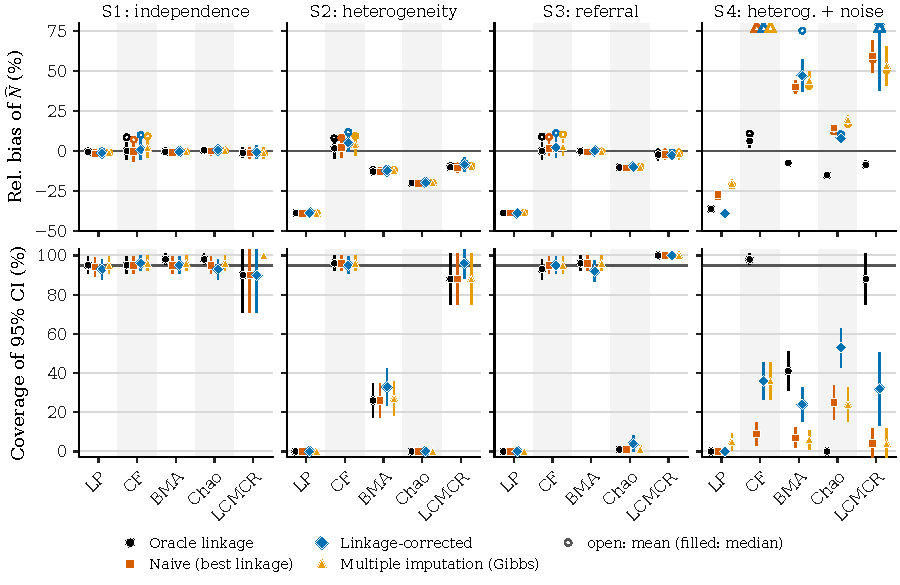
\includegraphics[width=6in]{figures/fig-sim-bias-coverage.pdf}
\caption{Synthetic data, scenarios S1--S4. Top: median relative bias of $\Nhat$ (filled; bars $\pm2$ MCSE) and mean relative bias (open). Bottom: coverage of nominal $95\%$ intervals (bars $\pm2$ MCSE). Triangles on the upper edge mark values beyond the axis. Linkage-corrected: LE correction with audit rates, interval with $v_{\mathrm{link}}$. $R=100$; LCMCR on 10 (S1, S3) or 25 (S2, S4) replicates.}\label{fig:sim-bias-coverage}
\end{figure}

\begin{table}[t]
\centering
\caption{Synthetic data, scenarios S1--S4. Median (MAD): median relative bias of $\Nhat$ in $\%$, with $1.4826\times$ the median absolute deviation in percentage points. Mean: mean relative bias in $\%$; the superscript counts replicates with $\Nhat>5N$. Cov.: coverage of nominal $95\%$ intervals in $\%$. Corrected: LE correction with audit rates, interval with $v_{\mathrm{link}}$. MI: 20 Gibbs linkage draws with Rubin's rules. $R=100$; LCMCR on 10 (S1, S3) or 25 (S2, S4) replicates.}\label{tab:sim-main}
\setlength{\tabcolsep}{2.6pt}
\simfit{% Generated by code/make_figures.py from results/sim_results.json -- do not edit by hand.
% Bias: mean relative bias of N_hat (%); Cov.: coverage of nominal 95% intervals (%).
% Means of exploding estimators are outlier-dominated; medians are in results/sim_results.json.
% Replications R = {'S1': 100, 'S2': 100, 'S3': 100, 'S4': 100}; LCMCR replications = {'S1': 20, 'S2': 40, 'S3': 20, 'S4': 40}.
\begin{tabular}{@{}llrrrrrrrrrr@{}}
\toprule
 & & \multicolumn{2}{c}{LP} & \multicolumn{2}{c}{CF} & \multicolumn{2}{c}{BMA} & \multicolumn{2}{c}{Chao} & \multicolumn{2}{c}{LCMCR} \\
\cmidrule(lr){3-4} \cmidrule(lr){5-6} \cmidrule(lr){7-8} \cmidrule(lr){9-10} \cmidrule(lr){11-12}
Scenario & Pipeline & Bias & Cov. & Bias & Cov. & Bias & Cov. & Bias & Cov. & Bias & Cov. \\
\midrule
S1 & Oracle & $-$0.3 & 95 & $+$8.6 & 95 & $-$0.2 & 98 & $+$0.2 & 98 & $-$0.6 & 95 \\
 & Naive & $-$1.3 & 94 & $+$7.0 & 95 & $-$1.1 & 95 & $-$0.4 & 95 & $-$1.4 & 95 \\
 & Corrected & $-$0.5 & 93 & $+$9.0 & 95 & $-$0.3 & 95 & $+$0.4 & 93 & $-$0.8 & 95 \\
 & MI & $-$2.1 & 93 & $+$6.8 & 97 & $-$1.4 & 91 & $+$0.0 & 95 & $-$1.6 & 100 \\
\addlinespace
S2 & Oracle & $-$39.0 & 0 & $+$7.9 & 96 & $-$12.0 & 26 & $-$19.9 & 0 & $-$10.1 & 78 \\
 & Naive & $-$39.2 & 0 & $+$8.3 & 96 & $-$12.5 & 26 & $-$20.3 & 0 & $-$10.9 & 62 \\
 & Corrected & $-$39.0 & 0 & $+$11.3 & 93 & $-$11.6 & 31 & $-$19.7 & 0 & $-$9.5 & 85 \\
 & MI & $-$39.2 & 0 & $+$11.1 & 95 & $-$11.8 & 27 & $-$20.0 & 0 & $-$10.3 & 80 \\
\addlinespace
S3 & Oracle & $-$38.9 & 0 & $+$8.9 & 93 & $-$0.1 & 96 & $-$10.1 & 1 & $-$0.3 & 100 \\
 & Naive & $-$38.9 & 0 & $+$8.7 & 95 & $-$0.7 & 96 & $-$10.4 & 1 & $-$1.0 & 100 \\
 & Corrected & $-$38.9 & 0 & $+$10.4 & 94 & $+$0.0 & 95 & $-$9.9 & 3 & $+$0.5 & 100 \\
 & MI & $-$38.8 & 0 & $+$11.2 & 96 & $-$0.7 & 96 & $-$9.9 & 2 & $-$0.0 & 100 \\
\addlinespace
S4 & Oracle & $-$36.2 & 0 & $+$10.9 & 98 & $-$7.8 & 41 & $-$15.2 & 0 & $-$7.9 & 80 \\
 & Naive & $-$28.5 & 0 & $+$204.3 & 9 & $+$39.2 & 7 & $+$12.2 & 25 & $+$58.1 & 8 \\
 & Corrected & $-$38.4 & 0 & $>{+}10^4$ & 12 & $+$72.2 & 12 & $+$12.1 & 31 & $+$174.6 & 18 \\
 & MI & $-$29.0 & 0 & $+$238.7 & 27 & $+$63.0 & 14 & $+$12.7 & 28 & $+$53.3 & 12 \\
\bottomrule
\end{tabular}
}
\end{table}

\paragraph{(Q1) Heterogeneity and referral.} \Cref{fig:sim-bias-coverage} and \cref{tab:sim-main} summarise S1--S4.
\begin{itemize}
  \item \emph{S1 (independence, clean records).} Every estimator is close to unbiased. The oracle medians lie within $\pm1.2\%$, and the coverages lie between $0.90$ and $0.98$. Clean records are linked almost perfectly (pairwise precision and recall about $0.99$ in S1--S3), so every pipeline lies within $\pm2.0\%$. The closed form is unbiased in median ($-0.1\%$) but heavy-tailed: its mean is $+8.6\%$, and its median interval width is $1.09N$, against $0.10N$ for BMA. Chao's estimator is $+0.4\%$, close to its population limit of $+0.4\%$ under independent capture with unequal list probabilities, where \cref{prop:id-mt} makes it an upper bound.
  \item \emph{S2 (heterogeneity).} The estimators separate as \cref{sec:identification} predicts. LP is $-38.8\%$, against a population limit of $-39.2\%$; \cref{prop:id-hetero}(a) gives a downward bias for $K=2$. Chao's estimator is $-20.0\%$, against a limit of $-19.8\%$; \cref{thm:chao} makes it a lower bound here. BMA is $-12.9\%$ with coverage $0.26$, because BIC selects pairwise models that do not absorb the heterogeneity. The closed form is $+1.7\%$ in median, because the population top interaction is small ($\omega=-0.074$), but it remains heavy-tailed. LCMCR is correctly specified and is $-10.2\%$, with coverage $0.88$ (MCSE $0.065$, $R=25$). The low-visibility class holds half of the incidents and has capture probabilities of $0.06$--$0.15$, so four lists barely identify it (\cref{rem:models-lc-id}). The LCMCR fits in S2 also fail our convergence protocol (Q6).
  \item \emph{S3 (referral, $q=0.5$).} LP is $-38.8\%$, against the limit of $-38.7\%$ given by \eqref{eq:id-referral-bias}. Dropping the referral-only NGO records by their provenance flag (\cref{prop:referral}(c)) gives $-1.1\%$, with coverage $0.93$. The four-list estimators need no correction. BMA is $-0.2\%$ and the closed form $-0.0\%$, because the other two lists are independent of the referral channel (\cref{prop:referral}(e)). Chao's estimator is $-10.3\%$, and LCMCR $-2.3\%$.
  \item \emph{S7 (referral sweep, \cref{fig:sim-referral}).} At $q=0.25$, $0.5$, $0.75$ and $1$, LP on all records is $-26.3\%$, $-38.6\%$, $-45.9\%$ and $-50.4\%$, against limits of $-26.4\%$, $-38.7\%$, $-45.9\%$ and $-50.6\%$ from \eqref{eq:id-referral-bias}. After provenance recoding it lies between $-1.1\%$ and $-0.1\%$ for every $q$, with coverage $0.945$--$0.970$. BMA on all records is unbiased up to $q=0.75$, but at $q=1$ it is $-29.5\%$ with coverage $0.01$. Every police record then reaches the NGO, so the police-only cells are structurally empty and $\omega$ is undefined. Recoding repairs this as well ($-0.2\%$; \cref{tab:sim-referral}).
  \item \emph{S4 (oracle linkage).} With heterogeneity driven partly by covariates, LP is $-36.3\%$ and Chao's estimator $-15.1\%$. BMA is $-7.5\%$, with coverage $0.41$. LCMCR is $-8.7\%$, with coverage $0.88$. The closed form is $+6.2\%$, with coverage $0.98$ and a median width of $0.94N$. Q4 takes up the effect of linkage in S4.
\end{itemize}

\begin{figure}[t]
\centering
\begin{minipage}[b]{2.9in}
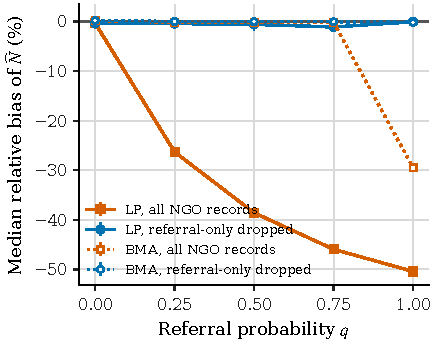
\includegraphics[width=2.9in]{figures/fig-sim-referral.pdf}
\end{minipage}\hfill
\begin{minipage}[b]{0.4\textwidth}
\caption{Synthetic data, S7 (independent capture, oracle linkage, $R=200$ per $q$). Median relative bias of $\Nhat$ against the referral probability $q$, using all NGO records or after dropping referral-only records by their provenance flag (\cref{prop:referral}(c)). Bars: $\pm2$ MCSE. Coverage is in \cref{tab:sim-referral}.}\label{fig:sim-referral}
\end{minipage}
\end{figure}

\begin{figure}[t]
\centering
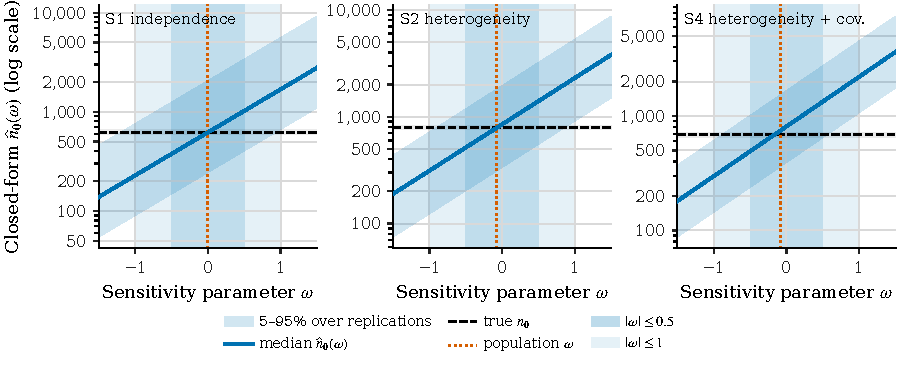
\includegraphics[width=6in]{figures/fig-sim-sensitivity.pdf}
\caption{Synthetic data, S6. Closed-form $\widehat n_{\zero}(\omega)$ on the oracle tables of S1, S2 and S4 ($R=100$): median curve and $5$--$95\%$ band over replicates, on a log scale. Shading: $|\omega|\le0.5$ and $|\omega|\le1$. Dashed: mean true $n_{\zero}$ (grey band: its $5$--$95\%$ range). Dotted: mean population $\omega$.}\label{fig:sim-sensitivity}
\end{figure}

\paragraph{(Q2) Sensitivity bands.} S6 applies the closed form \eqref{eq:id-closed} to the oracle tables (\cref{fig:sim-sensitivity}, \cref{tab:sim-sensitivity}). At $\omega=0$ its median error in $n_{\zero}$ is $-0.2\%$ (S1), $+4.1\%$ (S2), $-0.1\%$ (S3) and $+18.2\%$ (S4). The population top interaction is $0$ in S1 and S3, $-0.074$ in S2 and $-0.086$ in S4. For $K=4$, $\bar\omega=\omega$, so \cref{prop:direction} predicts that S2 and S4 overstate the dark figure, as they do. The asymptotic overstatement $e^{-\bar\omega}-1$ is $+7.7\%$ and $+9.0\%$, and the S4 median exceeds it.

The estimated bounds $[\widehat n_{\zero}(-\Omega),\widehat n_{\zero}(\Omega)]$ of \cref{cor:bounds}(b) contain $n_{\zero}$ in $87\%$ (S1), $93\%$ (S2), $87\%$ (S3) and $98\%$ (S4) of replicates for $\Omega=1$, and in $50$--$71\%$ for $\Omega=0.5$. These are point estimates of the identified set. They make no allowance for sampling error, and the closed form is noisy, so they can miss $n_{\zero}$ even when $|\omega|\le\Omega$ holds, as in S1 and S3. The union of the Wald intervals for $n_{\zero}$ over $|\omega|\le\Omega$ (the construction of \cref{cor:bounds}(c) with $c=z_{0.975}$) contains $n_{\zero}$ in $99$--$100\%$ of replicates for $\Omega=0.5$ and in $100\%$ for $\Omega=1$. The price is width. At $\Omega=1$ the bounds span a factor of $e^2\approx7.4$; the median bounds in S1 are $[228,1682]$, against a mean true $n_{\zero}$ of $622$. The bands therefore behave as the theory says. Without a substantive bound on $\omega$, however, they are too wide to inform policy. This is the identification problem of \cref{thm:nonid}, not a feature of the simulation.

\begin{figure}[t]
\centering
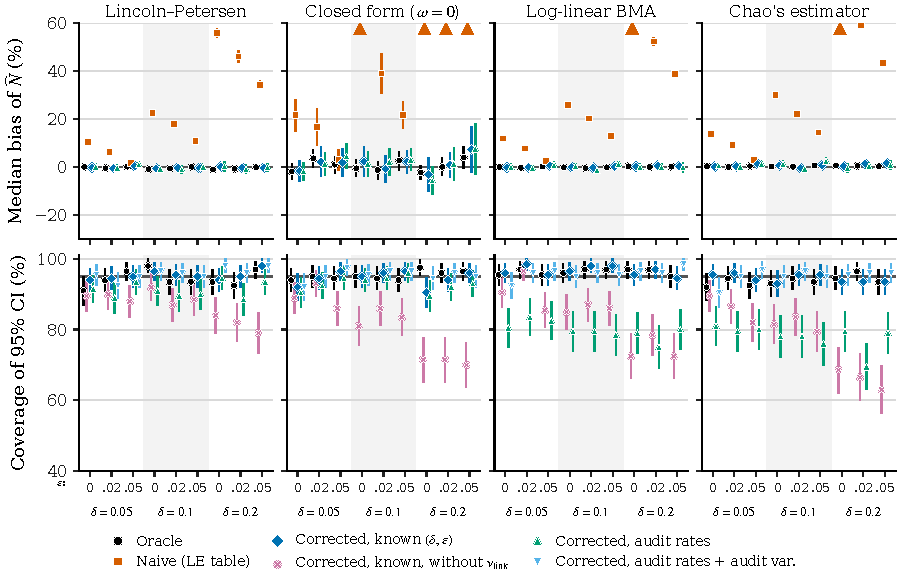
\includegraphics[width=6in]{figures/fig-sim-le-validation.pdf}
\caption{Synthetic data, S8: observed tables generated by the LE model (independent capture, $N=2000$, $R=200$ per $(\delta,\varepsilon)$ cell). Top: median relative bias of $\Nhat$ (bars $\pm2$ MCSE; triangles: off the axis). Bottom: coverage of nominal $95\%$ intervals (bars $\pm2$ MCSE). Known: correction with the true $(\delta,\varepsilon)$. Audit rates: rates from a simulated random audit (200 records, 100 linked edges).}\label{fig:sim-le-validation}
\end{figure}

\begin{table}[t]
\centering
\caption{Synthetic data, S8: the LE model generates the observed table (independent capture, $N=2000$, $R=200$ per cell; coverage MCSE about $1.5$ points). Naive: estimator applied to the LE table. Known: correction with the true $(\delta,\varepsilon)$. Audit: correction with audit-estimated rates (200 records, 100 linked edges). Known$^-$: interval without $v_{\mathrm{link}}$, as in the first run. Known and Audit: interval with $v_{\mathrm{link}}$. Audit$^+$: with the audit variance added.}\label{tab:sim-le}
\small
\setlength{\tabcolsep}{4pt}
\simfit{% Generated by code/make_figures.py from results/sim_results.json (run 2) -- do not edit by hand.
% S8: observed table = simulate_observed(t_true, delta, eps) (the LE model itself); independent capture,
% N = 2000, R = 200 per cell. Known: linkage_corrected with the true (delta, eps); Audit: rates from a
% random audit simulated from the LE ground truth (200 records + 100 linked edges). Known^-: interval without
% v_link (inner estimator only, as in run 1); Known/Audit: with v_link; Audit^+: + audit variance.
\begin{tabular}{@{}rrrrrrrrrrrrr@{}}
\toprule
 & & \multicolumn{3}{c}{BMA: median bias (\%)} & \multicolumn{5}{c}{BMA: coverage (\%)} & \multicolumn{3}{c}{Known rates: cov. with / without $v_{\mathrm{link}}$} \\
\cmidrule(lr){3-5}\cmidrule(lr){6-10}\cmidrule(lr){11-13}
$\delta$ & $\varepsilon$ & Naive & Known & Audit & Oracle & Known$^-$ & Known & Audit & Audit$^+$ & LP & CF & Chao \\
\midrule
0.05 & 0 & $+$11.9 & $-$0.2 & $-$0.1 & 96 & 90 & 96 & 80 & 92 & 94/90 & 92/89 & 96/90 \\
0.05 & 0.02 & $+$7.8 & $-$0.2 & $-$0.4 & 97 & 96 & 98 & 84 & 96 & 94/90 & 94/93 & 96/86 \\
0.05 & 0.05 & $+$2.4 & $+$0.5 & $+$0.8 & 96 & 86 & 96 & 82 & 96 & 95/88 & 96/86 & 94/82 \\
\addlinespace
0.1 & 0 & $+$25.9 & $-$0.1 & $+$0.1 & 96 & 85 & 96 & 80 & 95 & 96/92 & 95/81 & 93/82 \\
0.1 & 0.02 & $+$20.2 & $-$0.3 & $-$1.5 & 97 & 87 & 98 & 80 & 96 & 96/87 & 96/86 & 96/84 \\
0.1 & 0.05 & $+$12.9 & $+$0.1 & $+$1.1 & 97 & 86 & 98 & 78 & 96 & 95/88 & 96/84 & 96/80 \\
\addlinespace
0.2 & 0 & $+$62.7 & $+$0.2 & $-$0.1 & 97 & 72 & 96 & 79 & 96 & 94/84 & 90/72 & 94/68 \\
0.2 & 0.02 & $+$52.4 & $+$0.5 & $-$0.2 & 97 & 78 & 97 & 75 & 96 & 95/82 & 94/72 & 94/66 \\
0.2 & 0.05 & $+$38.9 & $+$0.3 & $-$0.3 & 95 & 72 & 94 & 80 & 98 & 98/79 & 96/70 & 94/63 \\
\bottomrule
\end{tabular}
}
\end{table}

\paragraph{(Q3) Does the LE correction work when its model holds?} Yes (S8; \cref{fig:sim-le-validation}, \cref{tab:sim-le}). Across the grid the naive BMA is biased by $+2.4\%$ to $+62.7\%$. The bias grows with $\delta$, and merging partly offsets it. With the true $(\delta,\varepsilon)$ the corrected estimators are median-unbiased: BMA lies between $-0.3\%$ and $+0.5\%$, LP between $-0.7\%$ and $+0.3\%$, Chao between $-0.4\%$ and $+1.5\%$, and the heavy-tailed closed form between $-3.2\%$ and $+7.3\%$. The intervals need $v_{\mathrm{link}}$. With it, BMA covers in $0.945$--$0.985$ of replicates, close to the oracle's $0.950$--$0.970$. Without it, as in the first run, BMA covers in only $0.725$--$0.965$, worst at $\delta=0.2$. LP and Chao behave alike: $0.940$--$0.980$ and $0.930$--$0.960$ with $v_{\mathrm{link}}$, and $0.790$--$0.920$ and $0.630$--$0.895$ without. The closed form drops to $0.905$ at $\delta=0.2$, $\varepsilon=0$, where its forward-difference gradient is inaccurate.

With audit-estimated rates the point estimates stay median-unbiased (BMA $-1.5\%$ to $+1.1\%$). The audit's own $95\%$ intervals cover the realised $\delta$ in $0.895$--$0.95$ of replicates and the realised $\varepsilon$ in $0.91$--$0.93$. However, $v_{\mathrm{link}}$ alone now undercovers (BMA $0.750$--$0.835$, Chao $0.695$--$0.810$), because it ignores the audit error. Adding the audit variance of \cref{cor:linkcorrect}(iii) restores coverage: BMA $0.925$--$0.985$, LP $0.925$--$0.980$, CF $0.920$--$0.975$ and Chao $0.905$--$0.970$. As \cref{rem:link-sameaudit} predicts, the sum is conservative in some cells. It is also costly: the median BMA width is $0.17N$--$0.44N$, against $0.12N$--$0.22N$ with known rates.

\begin{figure}[t]
\centering
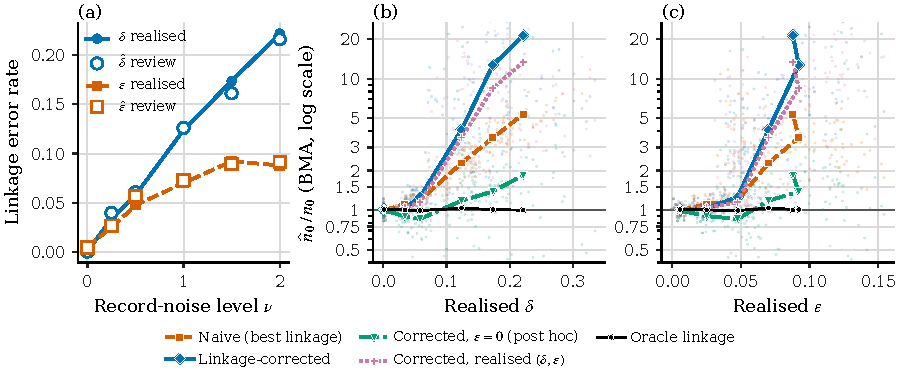
\includegraphics[width=6in]{figures/fig-sim-linkage-error.pdf}
\caption{Synthetic data, S5 (independent capture, record-noise sweep, $R=40$ per level). (a) Means over replicates of the realised capture-level rates $\delta$ and $\varepsilon$ of the point linkage, the same rates on the audit frame, and the audit estimates. (b, c) Dark-figure ratio $(\Nhat-n)/n_{\zero}$ for BMA against the realised $\delta$ and $\varepsilon$, on a log scale, where $n$ is the true number of recorded incidents. Points: replicates. Lines: medians by noise level. The $\varepsilon=0$ variant is post hoc.}\label{fig:sim-linkage-error}
\end{figure}

\begin{table}[t]
\centering
\caption{Synthetic data. BMA under realistic linkage: the S5 noise sweep (independent capture, $R=40$ per level) and S4 ($R=100$). Rates: means over replicates of the realised capture-level false-match rate $\varepsilon$ of the point linkage, its audit estimate $\hat\varepsilon$, and the best-fit $\varepsilon^\ast$. Remaining columns: median relative bias of $\Nhat$ in $\%$; the superscript counts replicates with $\Nhat>5N$. LE-corr.: audit rates. Realised: realised rates. $^\dagger$\,Post hoc variant, added after the first run. $^\ddagger$\,Infeasible diagnostic that uses the oracle table. Generated from \texttt{results/sim\_results.json}.}\label{tab:sim-realistic}
\small
\setlength{\tabcolsep}{4pt}
% Rows generated by a script from results/sim_results.json (run 2):
%   rates   = scenarios[S5|S4].results[i].linkage.{eps_true,eps_hat,lefit_eps}.mean
%   biases  = scenarios[...].estimates[pipeline].bma.relbias_median, pipelines
%             oracle, naive, corrected, corrected_true, corrected_d, corrected_lefit, mi
%   [k]     = estimates[pipeline].bma.n_blowup
\begin{tabular}{@{}lrrrrrrrrrr@{}}
\toprule
 & \multicolumn{3}{c}{False-match rate} & \multicolumn{7}{c}{Median relative bias of $\Nhat$ (\%)} \\
\cmidrule(lr){2-4}\cmidrule(lr){5-11}
 & $\varepsilon$ & $\hat\varepsilon$ & $\varepsilon^\ast$ & Oracle & Naive & LE-corr. & Realised & $\varepsilon{=}0^\dagger$ & Best-fit$^\ddagger$ & MI \\
\midrule
S5, $\nu=0$ & 0.006 & 0.006 & 0.010 & $+$0.7 & $\phantom{+}$0.0 & $+$0.4 & $+$0.8 & $-$0.2 & $+$0.5 & $+$0.1 \\
S5, $\nu=0.25$ & 0.025 & 0.023 & 0.011 & $+$0.3 & $+$4.5 & $+$1.5 & $+$1.8 & $-$3.1 & $-$0.3 & $+$8.7 \\
S5, $\nu=0.5$ & 0.048 & 0.051 & 0.015 & $-$0.2 & $+$7.2 & $+$7.5 & $+$4.5 & $-$5.0 & $-$0.7 & $+$17.1 \\
S5, $\nu=1$ & 0.070 & 0.072 & 0.008 & $+$0.6 & $+$40.4 & $+$63.4\textsuperscript{[1]} & $+$52.1 & $+$3.0 & $+$9.2 & $+$41.1 \\
S5, $\nu=1.5$ & 0.092 & 0.088 & 0.012 & $+$0.4 & $+$75.3 & $+$158.5\textsuperscript{[7]} & $+$219.7\textsuperscript{[5]} & $+$9.7 & $+$22.4 & $+$44.2 \\
S5, $\nu=2$ & 0.088 & 0.093 & 0.002 & $+$0.3 & $+$117.8 & $+$367.2\textsuperscript{[18]} & $+$306.9\textsuperscript{[14]} & $+$15.0 & $+$27.0 & $+$53.3 \\
\addlinespace
S4 & 0.077 & 0.079 & 0.000 & $-$7.5 & $+$40.0 & $+$47.1\textsuperscript{[1]} & $+$38.5 & $-$4.5 & $+$4.3 & $+$44.2 \\
\bottomrule
\end{tabular}
\end{table}

\paragraph{(Q4) Does it work under realistic linkage?} No (S4, S5; \cref{fig:sim-linkage-error}, \cref{tab:sim-realistic}). Take S4. The point linkage has pairwise precision $0.905$ and recall $0.787$. On average it misses $37.9$ of $91.6$ within-list duplicates and leaves $126.7$ more clusters than there are recorded incidents, so the naive BMA is $+40.0\%$ (coverage $0.07$). The audit estimates its targets well: $\hat\delta=0.107$ against $0.111$ on its frame, and $\hat\varepsilon=0.079$ against $0.081$, with interval coverage $0.96$ and $0.98$. Yet the LE-corrected BMA is $+47.1\%$ (mean $+75.3\%$, one blow-up), worse than naive. Its coverage is $0.24$, and $0.10$ without $v_{\mathrm{link}}$. With the audit variance, coverage rises to $0.76$, but only because the median interval is $2.36N$ wide. The corrected closed form is $+458.8\%$, with 54 blow-ups in 100 replicates.

The audit is not to blame. With the realised rates of the point linkage the correction still gives $+38.5\%$. What fails is the model. The best-fitting scalar LE has $\varepsilon^\ast=0.000$ in every S4 replicate (with $\delta^\ast=0.079$ on average), and in S5 its mean $\varepsilon^\ast$ lies between $0.002$ and $0.015$. Yet $7$--$9\%$ of singletons are falsely merged at $\nu\ge1$ and in S4.

The explanation is \emph{swaps}. Under the one-record-per-list constraint, a record whose true partner is degraded by noise is typically linked to a wrong partner from the same list. Suppose the true clusters are $\{a_1,a_2\}$ and $\{b_2\}$, where subscripts denote lists, and the linkage returns $\{a_1,b_2\}$ and $\{a_2\}$. The capture table is unchanged. LE has no move that links a record to the wrong partner. The audit, however, correctly counts this swap as one split true pair and one false edge, which raises both $\hat\delta$ and $\hat\varepsilon$. Inverting a merge rate that left no trace in the table then over-corrects. Missed duplicates add singletons that LE does not model either (\cref{rem:link-dedup}).

The S5 sweep shows the transition. At $\nu=0.25$ the correction helps ($+1.5\%$ against $+4.5\%$ naive). At $\nu=0.5$ it is neutral ($+7.5\%$ against $+7.2\%$). From $\nu=1$ on it is worse than naive: $+63.4\%$, $+158.5\%$ and $+367.2\%$, against $+40.4\%$, $+75.3\%$ and $+117.8\%$.

Two further pipelines bracket what is achievable. The $\varepsilon=0$ variant is the best feasible pipeline in the study: $-4.5\%$ with coverage $0.69$ in S4, and between $-5.0\%$ and $+15.0\%$ across S5. But we chose it after seeing the first run. It ignores false matches that the audit shows to be frequent, and it would be wrong whenever false matches do change the table, as they do in S8. We report it as a post hoc observation, not as a validated method. The infeasible best-fit LE gives $+4.3\%$ with coverage $0.93$ in S4. At $\nu=1$, $1.5$ and $2$, however, it gives $+9.2\%$, $+22.4\%$ and $+27.0\%$, and its minimised Pearson distance grows from $0.3$ at $\nu=0$ to $143$ at $\nu=2$ (S4: $35$). So at high noise not even the best scalar $(\delta,\varepsilon)$ can represent the errors.

The answer to Q4 is that the LE correction is a stylised forward model. It is valid when the errors are LE-like (Q3), and a random audit cannot by itself tell whether they are. A feasible way to diagnose this is to fit ``table-effective'' rates on audited clusters, the feasible analogue of $(\delta^\ast,\varepsilon^\ast)$, and compare them with $(\hat\delta,\hat\varepsilon)$. A large gap in $\varepsilon$ signals swap-dominated errors. We have not implemented this diagnostic.

\begin{table}[t]
\centering
\caption{Synthetic data. MI with Gibbs linkage draws (approximate posterior under the plug-in FS pairwise model) against the point linkage. False merges, pairwise recall over all records, and $n-n^\star$ (clusters minus true recorded incidents) are means over replicates; draw columns average the first 5 draws of each replicate. BMA bias and coverage as in \cref{tab:sim-main}. S4: $R=100$; S5: $R=40$ per level.}\label{tab:sim-mi}
\small
% Generated by code/make_figures.py from results/sim_results.json (run 2) -- do not edit by hand.
% MI with Gibbs linkage draws (approximate posterior under the plug-in FS pairwise model) vs the point
% linkage. False merges, recall (pairwise, all records) and n - n* (observed clusters minus true observed
% incidents): means over replicates (draw columns: mean over the first 5 draws per replicate).
\begin{tabular}{@{}lrrrrrrrrrr@{}}
\toprule
 & \multicolumn{2}{c}{False merges} & \multicolumn{2}{c}{Recall} & \multicolumn{2}{c}{$n-n^\star$} & \multicolumn{2}{c}{BMA median bias (\%)} & \multicolumn{2}{c}{Cov. (\%)} \\
\cmidrule(lr){2-3}\cmidrule(lr){4-5}\cmidrule(lr){6-7}\cmidrule(lr){8-9}\cmidrule(lr){10-11}
Scenario & Point & Draw & Point & Draw & Point & Draw & Naive & MI & Naive & MI \\
\midrule
S4 & 98 & 112 & 0.787 & 0.710 & $+$127 & $+$178 & $+$40.0 & $+$44.2 & 7 & 6 \\
S5, $\nu=0$ & 5 & 7 & 0.998 & 0.993 & $-$4 & $-$2 & $-$0.0 & $+$0.1 & 92 & 95 \\
S5, $\nu=0.25$ & 25 & 27 & 0.932 & 0.898 & $+$22 & $+$41 & $+$4.5 & $+$8.7 & 55 & 28 \\
S5, $\nu=0.5$ & 52 & 54 & 0.884 & 0.816 & $+$31 & $+$71 & $+$7.2 & $+$17.1 & 45 & 10 \\
S5, $\nu=1$ & 102 & 113 & 0.760 & 0.674 & $+$75 & $+$112 & $+$40.4 & $+$41.1 & 2 & 12 \\
S5, $\nu=1.5$ & 164 & 187 & 0.669 & 0.585 & $+$83 & $+$107 & $+$75.3 & $+$44.2 & 0 & 15 \\
S5, $\nu=2$ & 208 & 247 & 0.581 & 0.509 & $+$113 & $+$115 & $+$117.8 & $+$53.3 & 0 & 20 \\
\bottomrule
\end{tabular}

\end{table}

\paragraph{(Q5) Multiple imputation against the point linkage.} In S1--S3 the records are clean, and MI, naive and oracle agree (\cref{tab:sim-main}). Under noise MI does not beat the naive table except at the highest noise levels (\cref{tab:sim-mi}). In S4 the BMA is $+44.2\%$ under MI against $+40.0\%$ naive, with coverage $0.06$ and $0.07$. In S5, MI is worse at $\nu=0.25$ and $0.5$ ($+8.7\%$ against $+4.5\%$, and $+17.1\%$ against $+7.2\%$) and about equal at $\nu=1$ ($+41.1\%$ against $+40.4\%$). Only at $\nu=1.5$ and $2$ is it better ($+44.2\%$ against $+75.3\%$, and $+53.3\%$ against $+117.8\%$), and even there coverage is only $0.15$--$0.20$.

The reason is visible in the draws. They split more true clusters than the point linkage. In S4 their pairwise recall is $0.710$ against $0.787$, and they leave $177.6$ surplus clusters against $126.7$. MI therefore propagates uncertainty around a worse-centred table. This does not contradict \cref{prop:totalvar}(iv), which assumes exact draws from a correct linkage posterior; a plug-in, pairwise-composite target is neither. The sampler itself mixes quickly. In S4 the lag-1 autocorrelation of the number of links across sweeps is $-0.033$, and about $343$ of $2186$ active records change cluster in each sweep. The problem is the target, not the mixing. The Bernoulli-and-greedy imputation of the first run was worse ($+64.5\%$; \cref{tab:sim-run12}). We did not try a fully Bayesian linkage model, or calibrating $\pi$ on the audit sample.

\begin{table}[t]
\centering
\caption{Synthetic data. LCMCR convergence diagnostics for the oracle and naive tables (4 chains $\times$ 7500 iterations, burn-in 2500, thinning 5; overdispersed starting values). Diagnostics are for $N$: rank-normalised split-$\widehat R$ and bulk/tail ESS \citep{vehtari2021}. \% protocol: share of fits meeting \cref{app:comp-diag} ($\widehat R<1.01$, bulk and tail ESS $\ge400$). Bias and coverage in $\%$, MCSE in parentheses.}\label{tab:sim-lcmcr}
\setlength{\tabcolsep}{3pt}
\simfit{% Generated by code/make_figures.py from results/sim_results.json (run 2) -- do not edit by hand.
% LCMCR fits with 4 chains x 7500 iterations (2500 burn-in, thin 5; 4000 pooled draws), overdispersed n0 starts.
% Rank-normalised split-Rhat and bulk / tail ESS of N (Vehtari et al. 2021). % protocol: fits meeting App. app:comp-diag
% (Rhat < 1.01 and bulk and tail ESS >= 400). Bias and coverage in %, Monte Carlo SE in parentheses.
\begin{tabular}{@{}llrrrrrrrrrr@{}}
\toprule
Scen. & Table & Fits & $\widehat R$ med. & $\widehat R$ max & \% $\widehat R{<}1.01$ & ESS$_b$ med. & ESS$_b$ min & ESS$_t$ med. & \% protocol & Median bias (MCSE) & Cov. (MCSE) \\
\midrule
S1 & Oracle & 10 & 1.002 & 1.004 & 100 & 2848 & 1479 & 3239 & 100 & $-$1.2 (1.6) & 90 (9) \\
S1 & Naive & 10 & 1.001 & 1.031 & 90 & 2990 & 161 & 3198 & 80 & $-$1.4 (1.7) & 90 (9) \\
S2 & Oracle & 25 & 1.042 & 1.240 & 8 & 95 & 13 & 168 & 0 & $-$10.2 (1.1) & 88 (6) \\
S2 & Naive & 25 & 1.048 & 1.341 & 8 & 105 & 10 & 179 & 0 & $-$10.6 (1.4) & 88 (6) \\
S3 & Oracle & 10 & 1.018 & 1.232 & 10 & 234 & 13 & 243 & 10 & $-$2.3 (1.9) & 100 (0) \\
S3 & Naive & 10 & 1.008 & 1.033 & 60 & 407 & 145 & 700 & 40 & $-$2.1 (1.7) & 100 (0) \\
S4 & Oracle & 25 & 1.031 & 1.197 & 8 & 174 & 15 & 231 & 4 & $-$8.7 (0.8) & 88 (6) \\
S4 & Naive & 25 & 1.024 & 1.278 & 12 & 140 & 11 & 191 & 0 & $+$59.3 (5.0) & 4 (4) \\
\bottomrule
\end{tabular}
}
\end{table}

\paragraph{(Q6) LCMCR computation.} Each LCMCR fit uses four chains of 7500 iterations, with burn-in 2500 and thinning 5, from overdispersed starting values for $n_{\zero}$, giving 4000 pooled draws. \Cref{app:comp-diag} requires $\widehat R<1.01$ and bulk and tail effective sample sizes of at least 400. All S1 oracle fits meet this protocol, and $80\%$ of the S1 naive fits. The S2 and S4 fits do not (\cref{tab:sim-lcmcr}). Only $8$--$12\%$ of them reach $\widehat R<1.01$. Their median $\widehat R$ is $1.024$--$1.048$, with maxima up to $1.341$, and their median bulk ESS is $95$--$174$. Only $0$--$4\%$ meet the protocol, and in S3 $10\%$ (oracle) and $40\%$ (naive) do. The LCMCR results for S2--S4 therefore come from a reduced protocol and must be read as such. The corrected and MI fits pool one chain per imputation, so they have no $\widehat R$.

Two pieces of evidence suggest that the shortfall does not drive the reported biases. First, the four chain medians of a fit differ by a median of $2.9\%$ of $N$ in S2 (maximum $13.2\%$), about $2\%$ in S4 with oracle linkage (maximum $7.4\%$) and $5.9\%$ in S4 with naive linkage (maximum $20.6\%$). The first two are small next to the oracle biases of $-10.2\%$ and $-8.7\%$. Second, the first run, with single chains of 6000 iterations on 40 replicates, gave similar medians: $-11.2\%$ in S2 and $-8.3\%$ in S4 (\cref{tab:sim-run12}). This is evidence, not proof. LCMCR should not be used on real data until a run meets the protocol.

\subsection{What the simulation does and does not show}\label{sec:sim-scope}

The simulation shows four things. First, the identification results of \cref{sec:identification} hold in finite samples. Referral and heterogeneity bias Lincoln--Petersen by close to their population limits. Provenance recoding, or lists unconnected to the referral channel, remove the referral bias. Chao's estimator falls below $N$ under incident heterogeneity and slightly above it under list heterogeneity. Second, when LE holds, the correction of \cref{cor:linkcorrect} removes the bias, and its intervals are calibrated once $v_{\mathrm{link}}$ and the audit variance are included. Third, under realistic FS-EM linkage the same correction with well-estimated rates over-corrects, because the errors are dominated by swaps that scalar LE cannot represent. Fourth, multiple imputation from a plug-in pairwise posterior does not repair a biased linkage.

The simulation does not show the following.
\begin{itemize}
  \item It says nothing about real lists. The worlds are not calibrated to any source, and there is one population size ($N=2000$) and one number of lists ($K=4$). Calibration is part of the analysis plan (\cref{sec:plan}).
  \item It does not evaluate the fully Bayesian linkage of \cref{alg:pipeline}, with uncertain $m$ and $u$ and duplicates resolved jointly, nor the targeted review of \cref{alg:review}.
  \item It does not evaluate a feasible estimator of table-effective linkage rates.
  \item It does not evaluate the covariate, small-area and funnel models of \cref{sec:models-cov,sec:models-sae,sec:funnel}.
  \item Its LCMCR results for S2--S4 rest on a sampler that does not meet our own convergence protocol, and LCMCR is never refitted over a grid of $\omega$ or $q$.
\end{itemize}
The post hoc $\varepsilon=0$ variant performed best under realistic linkage, but nothing here licenses it as a default.
}{}
\IfFileExists{sections/09-analysis-plan.tex}{\section{A pre-registered analysis plan}\label{sec:plan}

This section is the analysis plan we will register, time-stamped and with the commit hash of the analysis code, before any real record is accessed \citep{nosek2018}. It commits in advance to the estimand, the lists, the linkage protocol, the model-selection rule, the sensitivity grid, the validation checks and the decision rules. Any departure will be reported as a deviation, with its reason. The estimators are the ones implemented and tested on synthetic data in \cref{sec:simulation}. The plan contains no real-data results.

\subsection{Estimands}\label{sec:plan-estimands}

\paragraph{Primary estimand}
$N_d$ is the number of \emph{criminal antisemitic incidents}, under the harmonised scope of \cref{sec:src-harmonise}, occurring in a pilot domain $d$ (a jurisdiction and a period). The candidate pilot jurisdiction is New York City. Its police list is public at complaint level with an anti-Jewish bias field (\cref{sec:src-local}), and two of the other candidate lists operate there. The candidate period is the two calendar years 2024--2025. These begin after the October 2023 change in the ADL Audit's scope rule (\cref{sec:src-audit}), so the domain does not straddle it. Before registration, we will check that window for known interruptions in any list's reporting system and fix the final jurisdiction and period. Both choices remain candidates until then.

\paragraph{Secondary estimands}
\begin{enumerate}[(i)]
  \item The dark figure $\nzero=N_d-n$ and the dark-figure ratio $D_1=N_d/n_{1+}$ relative to the police list.
  \item The list coverages $p_k=n_{k+}/N_d$ for $k\in\Kset$, and in particular $p_1$. Because the pilot police list is local (NYPD) rather than federal, $p_1$ corresponds to $\rvic\rpol\rcls$ in the funnel of \cref{prop:funnel}. Comparing NYPD with NIBRS records for the same domain estimates $\rsub$ separately.
  \item $N_d$ by conduct class (assault; threat or intimidation; property damage), if each class has enough linked records to pass the checks in \cref{sec:plan-validation}.
  \item Scope variants: $N_d$ computed with and without incidents carrying the Israel/Zionism content flag (\cref{sec:src-harmonise}), reported side by side with no preferred variant.
  \item Exploratory: borough-by-year counts $N_{s,t}$ from the small-area model (\cref{eq:smallarea}), released only under the disclosure rules of \cref{sec:ethics}.
\end{enumerate}

\subsection{Lists and data-sharing agreements}\label{sec:plan-lists}

\Cref{tab:plan-lists} lists the records we will request. The public files (NYPD open data, the H.E.A.T. Map) are not sufficient for linkage. They lack the exact dates or exact locations that linkage needs, and they carry no provenance. They will be used only to check that the agreement extracts are complete. Every agreement will specify five things: purpose limitation; the minimum necessary fields; linkage inside a secure enclave using encoded identifiers (\cref{sec:ethics}); review of outputs for disclosure risk only, so that providers have no veto over substantive findings; and retention and destruction schedules. Data holders such as ADL and SCN are also stakeholders in the results. Pre-registration and the disclosure-only review clause protect the independence of the analysis.

\begin{table}[tbp]
\centering
\caption{Lists to be acquired for the candidate pilot (New York City). Fields marked $\dagger$ are held only inside the secure enclave (\cref{sec:ethics}).}\label{tab:plan-lists}
\footnotesize
\setlength{\tabcolsep}{4pt}
\renewcommand{\arraystretch}{1.15}
\begin{tabularx}{\textwidth}{@{}l>{\raggedright\arraybackslash}p{2.4cm}>{\raggedright\arraybackslash}X>{\raggedright\arraybackslash}p{3.3cm}@{}}
\toprule
$k$ & Holder & Fields requested & Agreement \\
\midrule
1 & NYPD; NIBRS extract for the same agencies & Complaint ID; date and time; geocoded location$^\dagger$; offence; bias code(s); target type; narrative$^\dagger$; date submitted to state/FBI & Research data-use agreement; IRB approval \\
\addlinespace
2 & ADL & Incident ID; date; location$^\dagger$; ADL category; narrative$^\dagger$; \textbf{provenance} (victim, police, media, named partner); content flag & Data-use agreement; disclosure-only output review \\
\addlinespace
3 & SCN & Log ID; date; location$^\dagger$; type; narrative$^\dagger$; whether referred to law enforcement; whether shared with ADL & Data-use agreement \\
\addlinespace
4 & Campus or community self-report portal(s) & Report ID; date; location$^\dagger$; conduct; bias category identifying anti-Jewish bias; narrative$^\dagger$ & Agreement with each operator \\
\addlinespace
aux & BJS (NCVS); Dept.\ of Education (Clery) & Published hate-crime reporting estimates; institution-level religion-bias counts & Public; no agreement needed \\
\bottomrule
\end{tabularx}
\end{table}

\subsection{Linkage protocol}\label{sec:plan-linkage}

\begin{enumerate}[1.]
  \item \emph{Ontology coding.} Two coders independently code every record on the five axes of \cref{sec:src-harmonise}, blind to the other lists, and a third resolves disagreements. Scope is decided per record before linkage.
  \item \emph{Within-list deduplication.} After this step each list holds at most one record per incident, as the framework requires (\cref{sec:framework}).
  \item \emph{Standardisation and encoding.} Dates are standardised to the day. Locations are geocoded and then encoded together with institution names, using the privacy-preserving encodings of \cref{sec:ethics}. Narratives never leave the enclave.
  \item \emph{Blocking and comparison.} Candidate pairs are restricted to the same or adjacent precinct and a date difference of at most 14 days. The comparison vector $\gamma_{rr'}$ has levels for date difference (0, 1, 2--3, 4--14 days), distance band, conduct agreement, target-type agreement and encoded-location similarity.
  \item \emph{Model-based linkage.} The parameters $m(\gamma)$ and $u(\gamma)$ are estimated by \cref{alg:fsem} \citep{fellegi1969}. The posterior over the linkage structure $\Link$ is sampled using the Bayesian multi-list matching of \cref{sec:linkage} \citep{sadinle2017,steorts2016}.
  \item \emph{Clerical review.} Uncertain links are reviewed following \cref{alg:review}, with the review budget allocated as in \cref{thm:review}. Each reviewed pair is judged by two reviewers who do not know which estimate it would move. We report Cohen's $\kappa$ and adjudicate disagreements.
  \item \emph{Linkage error and propagation.} The rates $\delta$ and $\varepsilon$ are estimated from the reviewed sample. They enter the correction of \cref{cor:linkcorrect}, and linkage uncertainty is propagated into $N_d$ by \cref{alg:pipeline}. \Cref{prop:totalvar} gives the variance decomposition we report.
  \item \emph{Freeze.} The linkage is frozen, and its diagnostics are archived, before any estimate of $N_d$ is computed (\cref{sec:plan-decisions}).
\end{enumerate}

\subsection{Models and the model-selection rule}\label{sec:plan-models}

The following are fixed in advance.
\begin{description}[style=unboxed,leftmargin=0pt]
  \item[M1, primary.] Latent-class multiple-systems estimation with a Dirichlet-process prior (\cref{eq:lcmcr}; \citealp{manriquevallier2016}). It includes the covariates conduct class, target type and setting, uses the prior specification of \cref{sec:models} with truncation $J^\star=10$, and propagates linkage uncertainty as in \cref{alg:pipeline}.
  \item[M2, secondary.] Bayesian model averaging over hierarchical log-linear models with all main effects and up to two-way interactions, weighted by BIC, with $\omega=0$ (\cref{thm:closed}; \citealp{fienberg1972,madigan1997}).
  \item[M3, bound.] The estimator of \cref{thm:chao} \citep{chao1987}, reported in every case. It is a lower bound under heterogeneity across incidents (model $M_h$) but can exceed $N$ when capture probabilities differ across lists (\cref{prop:id-mt}), so it is reported as a diagnostic reference, not as a floor.
\end{description}
\emph{Campus stratum.} List~4 operates only on campus. In M1 and M2, non-campus incidents therefore carry a declared structural zero for list~4: the campus stratum is estimated from all four lists and the non-campus stratum from lists 1--3 (\cref{ex:src-scope}; \cref{asm:fw-scope}). $N_d$ is the sum of the two.

\emph{Selection rule.} M1 is the primary model if it passes the posterior predictive check of \cref{sec:plan-validation}. If M1 fails and M2 passes, M2 becomes primary. If both fail, we report no point estimate of $N_d$, only M3 and the bounds of \cref{cor:bounds}. If the posterior median of the primary model falls below M3, we flag the result for review. Under $M_h$ this indicates negative dependence or misfit; under list heterogeneity it may instead reflect the upward bias of M3 (\cref{prop:id-mt}). The flag does not change the primary model. Strata are fixed as above. No list, stratum or covariate is added or removed after estimates are seen.

\subsection{Sensitivity analyses}\label{sec:plan-sensitivity}

The primary model is refitted over the full grid in \cref{tab:plan-sens}, $5\times5\times4\times4=400$ cells. The ``plausible region'' is declared in advance. It is used only in the decision rules of \cref{sec:plan-decisions} and does not restrict what is reported. If the provenance fields yield an estimate $\hat q$, we add $\hat q$ and its 90\% interval endpoints to the $q$ grid. We also vary the scope-coding rule (record-level majority versus any-record), the Dirichlet-process concentration prior, and the truncation level ($J^\star\in\{10,20\}$). We report the posterior median and 90\% interval of $N_d$ for every cell. We also report \emph{tipping points}: the smallest $|\omega|$, and separately the smallest $q$, at which a conclusion under the decision rules would change.

\begin{table}[tbp]
\centering
\caption{Pre-specified sensitivity grid. $\omega$: highest-order log-linear interaction (\cref{thm:closed,cor:bounds}); $q$: referral fraction from the police list to the audit (\cref{prop:referral}); $\delta,\varepsilon$: false non-match and false match rates of the linkage operator $\Lop(\delta,\varepsilon)$ (\cref{thm:linkbias}).}\label{tab:plan-sens}
\small
\begin{tabular}{@{}lll@{}}
\toprule
Parameter & Grid values & Plausible region \\
\midrule
$\omega$ & $-1,\ -0.5,\ 0,\ 0.5,\ 1$ & $|\omega|\le 0.5$ \\
$q$ & $0,\ 0.05,\ 0.10,\ 0.20,\ 0.30$ (plus $\hat q$ if estimable) & $q\le 0.20$ \\
$\delta$ & $0,\ 0.05,\ 0.10,\ 0.20$ & $\delta\le 0.10$ \\
$\varepsilon$ & $0,\ 0.01,\ 0.02,\ 0.05$ & $\varepsilon\le 0.02$ \\
\bottomrule
\end{tabular}
\end{table}

\subsection{Validation}\label{sec:plan-validation}

\paragraph{Calibration before unblinding}
Before fitting real data, we rerun the simulation pipeline of \cref{sec:simulation} on synthetic worlds calibrated to the observed list sizes and to the estimated $(\delta,\varepsilon)$. The primary model must attain at least 85\% empirical coverage for its nominal 90\% intervals. If it does not, its intervals will be reported as uncalibrated.

\paragraph{Held-out-list prediction}
For each $k\in\Kset$, we fit the selected model to the other $K-1$ lists to obtain a posterior for $N_d$. Let $n_{-k}$ be the number of incidents those lists capture. Suppose list $k$ captures incidents with a common probability, independently of capture by the other lists. Then, given $n_{k+}$, the set of incidents list $k$ captures is a uniformly random subset of $U_d$. The number $m_k$ of list-$k$ records linked to at least one other list is therefore hypergeometric:
\begin{equation}\label{eq:plan-holdout}
  m_k \mid N_d,\,n_{-k},\,n_{k+} \;\sim\; \operatorname{Hypergeometric}\bigl(N_d,\; n_{-k},\; n_{k+}\bigr)\;\approx\;\Bin\!\left(n_{k+},\; n_{-k}/N_d\right).
\end{equation}
We report the posterior predictive $p$-value of the observed $m_k$. The check tests the $(K-1)$-list model and the independence and homogeneity of list $k$ jointly. A small $p$-value (excess overlap) points to positive dependence such as referral. A large one (deficit) points to specialisation. Results are reported for each $k$ separately.

\paragraph{Triangulation against NCVS reporting rates}
For hate crime in general, BJS publishes NCVS estimates of the share of victimisations reported to police \citep{bjs2021hate}. Write $r$ for the most recent such estimate at registration and $r^{+}$ for the upper end of its 95\% interval. Recording requires reporting, so we expect $p_1\le r$ approximately. The approximation is needed because the NCVS excludes institutional victims and is not specific to anti-Jewish bias (\cref{sec:src-surveys}). We report $\Pr(p_1>r^{+}\mid\text{data})$, and a value above $0.5$ is flagged. A flag would suggest scope mismatch, false matches that inflate overlaps, or unmodelled negative dependence. The ratio $p_1/r$ also gives a rough cross-check on $\rcls$ in \cref{prop:funnel}. This check triangulates; it does not identify $N_d$.

\paragraph{Posterior predictive check}
Following \citet{gelman2013}, we draw replicated capture tables from the posterior and compare them with the observed table through the Freeman--Tukey discrepancy over observed histories,
\begin{equation}\label{eq:plan-ft}
  T(\bm n,\bm\mu)=\sum_{\h\in\Hobs}\bigl(\sqrt{n_{\h}}-\sqrt{\mu_{\h}}\bigr)^2,
\end{equation}
as well as through the frequency counts $f_j$ and the list sizes $n_{k+}$. A model passes if the posterior predictive $p$-value of $T$ lies in $[0.05,0.95]$.

\subsection{Decision rules}\label{sec:plan-decisions}

These rules state which results would change our conclusions. They are fixed now.
\begin{enumerate}[D1.]
  \item \emph{Linkage gate.} If the review-based posterior mean of $\varepsilon$ exceeds $0.05$ or that of $\delta$ exceeds $0.20$, we do not estimate $N_d$. We revise blocking and comparisons and repeat the review, reporting this as a deviation.
  \item \emph{Ontology gate.} If Cohen's $\kappa$ for the in-scope decision is below $0.6$ for any list, on a random sample of at least 200 records (or all of them if fewer), scope-specific estimates are labelled exploratory.
  \item \emph{Model adequacy.} Applied as in \cref{sec:plan-models}. If no model passes, we report only bounds.
  \item \emph{Referral switch.} If list~2's held-out-list check shows excess overlap ($p<0.05$), or if the provenance data give $\hat q>0.10$ with a 90\% interval excluding $0.05$, the referral-adjusted model of \cref{prop:referral} replaces M1 as primary.
  \item \emph{Substantive statements.} We will say that the police list misses \emph{most} in-scope incidents only if $\Pr(p_1<0.5\mid\text{data})\ge 0.95$ under the primary model \emph{and} the posterior median of $p_1$ is below $0.5$ throughout the plausible region of \cref{tab:plan-sens}. We will say it captures most of them under the symmetric condition. If a statement holds under the primary model but fails somewhere in the plausible region, we report it as dependent on unverifiable assumptions and name the tipping point.
  \item \emph{Negative result.} If the held-out-list check fails for two or more lists, or the NCVS triangulation is flagged, we will conclude that these lists do not support MSE in the pilot domain. That conclusion will be reported with the same prominence as an estimate.
\end{enumerate}

\subsection{Reporting and replication}\label{sec:plan-reporting}

The report will contain the following.
\begin{itemize}
  \item A flow diagram of records, from received, to in scope, to deduplicated, to linked.
  \item The capture-history table, subject to the disclosure rules of \cref{sec:ethics}.
  \item Linkage diagnostics: estimated $(\delta,\varepsilon)$, review agreement, and the variance decomposition of \cref{prop:totalvar}.
  \item Estimates from M1--M3, the full sensitivity grid and the tipping points.
  \item All validation results.
  \item A log of deviations from this plan.
\end{itemize}
Our reporting follows the good-practice discussions in \citet{bird2018} and \citet{lum2013}. The replication package will contain the version-tagged \texttt{darkfig} code with deterministic seeds; the ontology codebook and coding manual; the clerical-review protocol; synthetic data with the same schema as the agreement extracts; and every released aggregate table. Record-level data cannot be redistributed. The package will document how qualified researchers can apply to the data holders for access under equivalent agreements.

\subsection{Timeline}\label{sec:plan-timeline}

\Cref{tab:plan-timeline} gives the phases. Month 0 is the date the plan is registered. Estimation begins only after the linkage freeze and the calibration study.

\begin{table}[tbp]
\centering
\caption{Phased timeline. Durations are planning targets, not commitments of the data holders.}\label{tab:plan-timeline}
\footnotesize
\renewcommand{\arraystretch}{1.15}
\begin{tabularx}{\textwidth}{@{}l l >{\raggedright\arraybackslash}X >{\raggedright\arraybackslash}p{3.6cm}@{}}
\toprule
Phase & Months & Activities & Exit criterion \\
\midrule
0. Registration & 0--3 & Register plan and code hash; IRB review; negotiate data-use agreements; convene community advisory group (\cref{sec:ethics}) & Plan registered; IRB approval; signed agreements \\
1. Acquisition & 3--8 & Receive extracts in enclave; ontology coding; within-list deduplication & Ontology gate D2 assessed \\
2. Linkage & 8--12 & Encoding; blocking; FS--EM and Bayesian matching; clerical review (\cref{alg:review}) & Linkage gate D1 passed; linkage frozen \\
3. Calibration & 12--14 & Calibrated simulation; blinded model fitting and diagnostics & Coverage check; model selection completed \\
4. Unblinding & 14--17 & Estimates, sensitivity grid, validation; disclosure review & Decision rules D3--D6 applied \\
5. Release & 17--20 & Briefings with community advisory group and data holders; manuscript; replication package & Public release \\
\bottomrule
\end{tabularx}
\end{table}
}{}
\IfFileExists{sections/10-ethics.tex}{\section{Ethics, privacy and responsible reporting}\label{sec:ethics}

The records this paper's methods are built for describe people at a moment of victimisation. A record reveals, or implies, a person's religion or perceived religion, the fact that they were targeted, and often where they live, work or worship. Some records also concern suspects, who may be minors and who have not been convicted. This section sets out the safeguards that the analysis plan of \cref{sec:plan} commits to. It also sets out the risks that remain even when the safeguards work.

\subsection{Consent, review and agreements}\label{sec:ethics-review}

None of the lists was compiled for research, and the people recorded in them did not consent to linkage. We will seek review by an institutional review board (IRB) before any data are transferred. We will ask the IRB to decide whether a waiver of consent is justified. That decision turns on whether the safeguards below keep risk minimal and whether contacting victims would itself cause harm. The data-use agreements of \cref{sec:plan-lists} restrict use to the registered protocol. They prohibit attempts at re-identification and any linkage beyond the protocol. They require the minimum necessary fields and set retention and destruction dates; linkage keys and encodings are destroyed when the replication package is released. Data holders review outputs for disclosure risk only. In the other direction, the agreements oblige us to notify data holders of any breach. Victim-service organisations will be consulted on whether research use should be disclosed to people who report in future, for example in the privacy notice of a reporting portal. Transparency of that kind may be worth a small cost in reporting rates, but the trade-off belongs to the community and to the data holders as well as to us.

\subsection{Privacy-preserving record linkage and its limits}\label{sec:ethics-pprl}

Linkage (\cref{sec:plan-linkage}) separates roles. Each data holder encodes the identifying fields (locations and institution names; names of persons are neither requested nor needed) and sends the encodings, with non-identifying attributes, to a linkage unit inside a secure enclave. Analysts receive only capture histories and covariates. Encoding uses Bloom filters \citep{schnell2009}. Each string is split into $q$-grams, each $q$-gram is mapped by several hash functions into a bit array, and the Dice coefficient of two bit arrays approximates the $q$-gram similarity of the underlying strings. This allows approximate matching without exchanging plaintext.

Bloom-filter encodings are not anonymous. Frequency-based cryptanalysis can recover encoded values when an attacker holds a reference list whose value frequencies resemble those of the encoded data. Published attacks include a constraint-satisfaction attack \citep{kuzu2011}, an attack on the individual bit patterns of basic Bloom filters \citep{niedermeyer2014}, and fast pattern-mining attacks \citep{christen2019}. Our setting is unfavourable in a specific way. The addresses of synagogues, schools and other Jewish institutions are public, and incidents that target institutions cluster on them. A reference list therefore exists for exactly the records whose exposure would be most harmful. We will treat encodings as personal data. They will be generated with keyed hash functions whose key is held by the data holders and not by the linkage unit. They will never leave the enclave, and they will be destroyed on schedule. Where an agreement permits matching on plaintext inside the enclave, we will prefer that, because it removes the attack surface without exporting anything.

\subsection{Enclaves, aggregate release and disclosure control}\label{sec:ethics-sdc}

All record-level processing, including clerical review, takes place in a secure research environment. Nothing leaves it without output review. Only aggregates are released. Every released table is subject to small-cell suppression with a minimum cell size $c$ fixed in the data-use agreements; we propose $c=10$ \citep{hundepool2012}. Capture-history tables need care beyond single-cell suppression, because the list holders publish their own totals. NYPD open data and the H.E.A.T. Map, for example, make list sizes $n_{k+}$ approximately public for a jurisdiction. A single suppressed cell $n_{\h}$ could then be recovered by subtraction from these margins. Complementary suppression, or release only of coarsened summaries such as the frequency counts $f_j$, will be applied so that no suppressed cell is determined by released and published totals together \citep{hundepool2012}. Small-area outputs (borough by year) are released only as model-based estimates with intervals. They are never released as maps of point locations.

\paragraph{Formal differential privacy (optional)}
For any released small-area counts, we may add a formal guarantee. A randomised mechanism $\mathcal M$ is $\varepsilon_{\mathrm{DP}}$-differentially private if, for every pair of datasets $D,D'$ that differ by the addition or removal of one incident, and for every measurable set $S$,
\begin{equation}\label{eq:eth-dp}
  \Pr\{\mathcal M(D)\in S\}\le e^{\varepsilon_{\mathrm{DP}}}\,\Pr\{\mathcal M(D')\in S\}
\end{equation}
\citep{dwork2006,dwork2014}. Here $\varepsilon_{\mathrm{DP}}$ is the privacy-loss parameter, unrelated to the false-match rate $\varepsilon$ of \cref{sec:linkage}. Each incident falls in exactly one cell of the capture-history table $(n_{\h})_{\h\in\Hobs}$, so the table has $\ell_1$-sensitivity~1 under this neighbouring relation. Adding independent $\mathrm{Laplace}(0,b)$ noise with $b=1/\varepsilon_{\mathrm{DP}}$ to every cell therefore satisfies \eqref{eq:eth-dp}. Each noisy cell has standard deviation $\sqrt2\,b=\sqrt2/\varepsilon_{\mathrm{DP}}$, and any estimate computed from the noisy table inherits the guarantee by post-processing \citep{dwork2014}. The guarantee protects incidents, not people. A person who was targeted several times is protected at level $m\,\varepsilon_{\mathrm{DP}}$, where $m$ is the number of incidents involving them.

The cost of this noise is best judged against the posterior uncertainty in $N$, not against the counts. MSE estimators depend on overlap cells through ratios, so the noise is amplified when overlaps are small. For the two-list Lincoln--Petersen estimator $\Nhat=n_{1+}n_{2+}/n_{11}$, suppose $n_{11}$ is small relative to the list sizes. To first order, the noise then adds a relative standard deviation of about $\sqrt2/(\varepsilon_{\mathrm{DP}}\,n_{11})$. The sampling relative standard deviation under independent, homogeneous capture is about $\{(1-p_1)(1-p_2)/n_{11}\}^{1/2}$. The ratio of the two is
\begin{equation}\label{eq:eth-ratio}
  \frac{\mathrm{SD}_{\mathrm{DP}}}{\mathrm{SD}_{\mathrm{samp}}}\;\approx\;\frac{\sqrt2}{\varepsilon_{\mathrm{DP}}\sqrt{n_{11}(1-p_1)(1-p_2)}}.
\end{equation}
As illustrative arithmetic, not a result, take $\varepsilon_{\mathrm{DP}}=1$ and $p_1=p_2=0.3$. For $n_{11}=50$ the ratio is about $0.29$, so the total standard deviation rises by about 4\%. For $n_{11}=5$ the ratio is about $0.90$, and the total standard deviation rises by about 35\%. Differential privacy is therefore cheap where MSE is informative and expensive where MSE is already weak, which is also where suppression applies. If we use it, inference will treat the noise-free table as latent and include the Laplace likelihood in the model of \cref{sec:models}. Naive plug-in estimates can fail when a noisy overlap cell is near zero.

\subsection{Errors in either direction}\label{sec:ethics-errors}

Both overestimation and underestimation of the dark figure cause harm, and the methods can err either way. False non-matches split incidents and shrink overlaps, which pushes $\Nhat$ up. False matches inflate overlaps and push it down (\cref{thm:linkbias}). Referral pushes the Lincoln--Petersen estimate down (\cref{prop:referral}). More generally, the sign of the oriented highest-order interaction determines the direction of the bias from unmodelled dependence (\cref{prop:direction}). Scope mismatch can push them either way (\cref{ex:src-scope}).

An overestimate can cause fear out of proportion to risk and misdirect scarce security resources. When it is later corrected, it can be used to discredit legitimate monitoring and the people who report.

An underestimate erases victims' experience and makes police data look more complete than they are, which can justify inaction.

We therefore commit to three practices. First, we report the heterogeneity-robust lower bound (\cref{thm:chao}) next to every estimate. Second, we report the full sensitivity grid rather than a single preferred cell. Third, we state the direction of each known bias source alongside the result.

\subsection{Communicating uncertainty}\label{sec:ethics-communication}

Estimates of unreported hate crime will be quoted without their caveats. Our release materials will therefore follow six rules.
\begin{enumerate}[(i)]
  \item Lead with an interval and a lower bound, not a point. For example: ``at least $L$; most plausibly between $A$ and $B$''.
  \item State the scope every time: criminal incidents, the jurisdiction and the period. Do not convert to ``percentage unreported'' without the interval.
  \item Do not compare one list's published total with another's as if they counted the same thing. The gap between an NGO audit and police statistics reflects scope and unit as well as under-reporting (\cref{sec:src-harmonise}).
  \item Do not describe changes over time across definitional or reporting-system breaks as trends. Examples are the NIBRS transition of 2021 and the Audit's scope change of October 2023 (\cref{sec:src-police,sec:src-audit}).
  \item Show sensitivity visually, for example as $\Nhat$ against $\omega$ with the plausible region shaded.
  \item Provide a plain-language summary, a frequently-asked-questions document, and embargoed briefings for journalists and officials that cover what the estimate does \emph{not} show.
\end{enumerate}

\subsection{Engagement with Jewish communities}\label{sec:ethics-community}

The work concerns a community that bears the harm being measured. Before data acquisition, we will convene an advisory group. It will include Jewish communal and security organisations, synagogue and campus organisations, and victim-service providers. It will also include privacy and civil-liberties experts and researchers who study hate crime against other groups, whose data infrastructures overlap with ours. The group will be consulted on three matters: the ontology and scope variants (\cref{sec:src-harmonise}), the disclosure rules, and how results are communicated. It has no veto over findings. Funding sources and any relationship between the research team and the data holders will be disclosed in every output. Communities differ in how they relate to the police and to communal organisations. Those differences are themselves sources of capture heterogeneity, so we will seek input across denominations, languages and neighbourhoods rather than through a single channel.

\subsection{Misuse}\label{sec:ethics-misuse}

We foresee four kinds of misuse.
\begin{itemize}
  \item \emph{Targeting.} Fine-grained maps of incidents or of ``under-reporting'' could point offenders to vulnerable institutions, or to areas where offences are least likely to be recorded. We therefore release no point locations and only coarse, model-based small-area outputs.
  \item \emph{Selective quotation.} One end of an interval, or one cell of the sensitivity grid, can be quoted to support a predetermined claim. The full grid and the decision rules of \cref{sec:plan-decisions} are published so that such quotation can be checked.
  \item \emph{Definitional proxy wars.} Scope variants with and without Israel/Zionism-related content will be reported side by side. They are not a ruling on any definition of antisemitism (\cref{sec:src-harmonise}).
  \item \emph{Function creep.} A linkage infrastructure built to count victims could be repurposed to monitor people, including those engaged in lawful protest. The agreements confine linkage to the registered protocol and require keys and encodings to be destroyed. No offender-level or protester-level dataset will be created.
\end{itemize}
}{}
\IfFileExists{sections/11-discussion.tex}{\section{Discussion}\label{sec:discussion}

\paragraph{What the framework makes possible}
The usual argument about antisemitic incidents asks whose count is right.
The framework replaces that question with a different one: what is the
population that every list samples, and how does each list sample it? Once
the target is defined (\cref{sec:framework}), the police count, an NGO audit
and a community-security log become \emph{data about} the same unknown
total, not competitors for it. Their overlaps are informative, their
dependence is modelled rather than assumed away (\cref{prop:referral}), and
the part of the answer that the data cannot deliver is isolated in a single
interpretable parameter $\omega$ (\cref{thm:closed,cor:bounds}). The
sensitivity frontier tells a reader how much unmeasured dependence a stated
conclusion can withstand (\cref{thm:id-frontier}). Linkage
error, which in practice is often handled silently, becomes an explicit
operator whose effect on the estimate can be quantified and corrected
(\cref{thm:linkbias,cor:linkcorrect}). Its residual uncertainty is carried
into the final interval (\cref{alg:pipeline}).

The funnel decomposition (\cref{prop:funnel,thm:shapley}) turns an estimate
of the dark figure into something a policymaker can act on. A gap between
two jurisdictions' recorded rates can arise because victims there are less
willing to come forward, because the police are less likely to recognise a
bias motivation, or because the agency does not submit its data. Each of
these calls for a different response: community outreach, officer training
or reporting infrastructure. Raw counts cannot tell these explanations apart.
The decomposition can, to the extent that the stage-specific rates are
identified by the auxiliary data of \cref{tab:funnel-sources}. Incidents that
were never disclosed to anyone remain beyond the reach of every list, so
that stage rests on victim surveys.

\paragraph{Limitations}
We stress five.

\emph{Untestable assumptions.} No method escapes the basic
non-identifiability of the unobserved cell (\cref{thm:nonid}). Our approach
makes the identifying assumption explicit and adjustable, but it does not
remove it. A sensitivity interval for $\omega$ is only as credible as the
range chosen for it, and that range must be argued from knowledge of how the
lists are generated, not from the data. It must in general be two-sided:
the model without a $K$-way interaction can overstate the dark figure as well
as understate it (\cref{prop:direction}, \cref{ex:id-hetero}). A one-sided
range is justified only by a mechanism of known sign, such as referral
between two lists (\cref{rem:id-calibrate}); with three or more lists,
referral itself can push the bias either way. Latent-class models replace the
assumption of no highest-order interaction with conditional independence
within classes. That is weaker in some directions and not in others. The
Chao bound is a lower bound only when heterogeneity runs across incidents.
Heterogeneity across lists can turn it into an upper bound
(\cref{prop:id-mt}), so it is a diagnostic, not a floor.

\emph{Scope harmonisation.} MSE requires every list to be sampling the same
population. The FBI records criminal offences with a recorded bias
motivation, whereas NGO audits also record non-criminal incidents under
their own and evolving criteria \citep{adl2025audit}. Harmonisation rules
(\cref{sec:src-harmonise,sec:plan}) can align the lists only as far as
their records contain the information needed to apply a common
definition. Residual mismatch
behaves like coverage error and cannot be fully separated from it.

\emph{Data access.} The methods assume record-level access to several
lists. Police records, NGO case files and community reports contain
sensitive information about victims who did not consent to being linked.
Obtaining such data will require data-sharing agreements,
privacy-preserving linkage \citep[e.g.,][]{schnell2009} and disclosure
control for small cells \citep{hundepool2012}, possibly with formal
privacy guarantees \citep{dwork2014}. Each of these degrades linkage
quality or precision to some degree. Encodings for privacy-preserving
linkage can themselves be attacked (\cref{sec:ethics-pprl}), and the ethics
protocol of \cref{sec:ethics} may rightly rule out some linkages
altogether.

\emph{The closed-population idealisation.} Incidents occur in continuous
time, lists have different reporting windows and lags, and records are
added or revised after the reference period ends. Treating each state--year
domain as a closed population is a convenient approximation. Its error is
concentrated at period boundaries and in lists with long reporting delays.

\emph{Approximate linkage-error models.} The operator
$\Lop(\delta,\varepsilon)$ assumes that detachments and false merges occur
independently across records, at rates that are at most list-specific
(\cref{rem:link-listspecific}). Real linkage errors
cluster: they are more frequent for incidents in dense places, for generic
incident descriptions and for records with missing fields, and they may be
correlated with capture history itself. The correction of
\cref{cor:linkcorrect} should therefore be read as a first-order adjustment.
Propagating linkage uncertainty by mixing over linkage draws
(\cref{alg:pipeline}) is preferable whenever record-level comparison data are
available. The modular posterior used there (\cref{eq:models-cut})
deliberately ignores the information that the capture model carries about
which records match, trading some efficiency for robustness.

\paragraph{Extensions}
Three extensions seem most valuable. First, \emph{open populations and
continuous time}: modelling incident occurrence as a point process and each
list as a time-varying, delayed thinning of it would remove the
closed-population idealisation and connect dark-figure estimation to
nowcasting of reporting delays. Second, \emph{online incidents}: here the
unit of analysis is itself unsettled, and platform moderation and automated
detection act as lists with their own selection and classification error, a
direct analogue of the funnel's classification stage. Third,
\emph{international comparison}. In the United Kingdom the Community Security Trust maintains a
long-running list of antisemitic incidents and documents the share it receives
from the police \citep{cst2026incidents}. The European Union Agency for
Fundamental Rights has surveyed Jewish people in several member states about
their experiences of antisemitism and about non-reporting
\citep{fra2018antisemitism,fra2024antisemitism}; see
\cref{sec:src-community,sec:src-surveys}. Combining such sources country by
country, with the funnel decomposition as a common accounting framework, would allow cross-national
comparisons of reporting, not only of recorded counts.

\paragraph{Why measure what is missing}
A count that omits its dark figure can mislead in both directions. Rising
counts may reflect greater willingness to report, better classification or
wider agency participation as much as rising incidence. Falling counts may
reflect lost trust or lapsed reporting. Resources allocated in proportion to
recorded incidents reward the communities and agencies that report, which
are not necessarily those that are most affected. Nor is there reason to
expect the dark figure to be random noise. If it is concentrated where victims
expect least from reporting, its size is itself a measure of the distance
between a community and the institutions meant to protect it. Estimating
it honestly, with explicit assumptions, propagated uncertainty and a plan fixed before the data are
seen, is how a measurement programme takes seriously the incidents that
nobody wrote down.
}{}

\bibliographystyle{plainnat}
\bibliography{refs,bib/sources,bib/theory,bib/linkage,bib/bayes,bib/lead}

\clearpage
\appendix
\IfFileExists{appendix/A1-identification-proofs.tex}{\section{Proofs for Section~\ref{sec:identification}}\label{app:idproofs}

Throughout, $\sum_{\h}$ and $\prod_{\h}$ without qualification run over $\Hobs$, and $\bar\omega=(-1)^K\omega$. We use the identities \eqref{eq:fw-signsum} and the key identity \eqref{eq:fw-key} repeatedly. For completeness, \eqref{eq:fw-key} follows from \eqref{eq:fw-omega} by isolating the term $T=\emptyset$:
\[
  \omega=(-1)^K\log\mu_{\zero}+\sum_{\h}(-1)^{K-|\h|}\log\mu_{\h}
  \;\Longrightarrow\;
  \log\mu_{\zero}=(-1)^K\omega-\sum_{\h}(-1)^{|\h|}\log\mu_{\h}=\bar\omega+\sum_{\h}s_{\h}\log\mu_{\h}.
\]
The Möbius sums \eqref{eq:fw-mobius} for $S\neq\emptyset$ annihilate additive constants, because $\sum_{T\subseteq S}(-1)^{|S|-|T|}=0$. Hence $\omega$ computed from $\bm\pi$ equals $\omega$ computed from $\bm\mu=N\bm\pi$, and \eqref{eq:fw-key} applies to $\bm\pi$. Writing $\bm\pi_+=(1-\pi_{\zero})\bm\pi^c$ and using the degree-one homogeneity of $\mathcal A$ gives \eqref{eq:fw-keyM}. Finally, \eqref{eq:fw-slice} follows by splitting the sum \eqref{eq:fw-omega} into the sets $T\not\ni k$, for which $(-1)^{K-|T|}=-(-1)^{K-1-|T|}$, and $T=T'\cup\{k\}$ with $T'\subseteq\Kset\setminus\{k\}$, for which $(-1)^{K-|T|}=(-1)^{K-1-|T'|}$.

\subsection{Preliminary lemmas}\label{app:id-prelim}

\begin{proof}[Proof of \cref{lem:id-param}]
Fix $\omega$. \emph{Injectivity.} Let $\bm u,\bm u'\in\Theta_\omega$ with $\bm\mu_+(\bm u)=\bm\mu_+(\bm u')$, and let $\bm\mu,\bm\mu'$ be the full mean vectors defined by \eqref{eq:fw-loglin}. Both satisfy \eqref{eq:fw-key} with the same $\omega$, so $\mu_{\zero}=e^{\bar\omega}\mathcal A(\bm\mu_+)=\mu'_{\zero}$. Hence $\bm\mu=\bm\mu'$ on all of $\Hset$, and $\bm u=\bm u'$ by \cref{lem:fw-mobius}.
\emph{Surjectivity.} Given $\bm\mu_+\in(0,\infty)^{\Hobs}$, set $\mu_{\zero}=e^{\bar\omega}\mathcal A(\bm\mu_+)$ and define $\bm u$ from the full vector $\bm\mu$ by \eqref{eq:fw-mobius}. By \cref{lem:fw-mobius}, $\bm u$ reproduces $\bm\mu$ through \eqref{eq:fw-loglin}, so $\bm\mu_+(\bm u)=\bm\mu_+$. Moreover,
\[
  u_{\Kset}=(-1)^K\log\mu_{\zero}+\sum_{\h}(-1)^{K-|\h|}\log\mu_{\h}
  =\omega+\sum_{\h}\bigl\{(-1)^Ks_{\h}+(-1)^{K-|\h|}\bigr\}\log\mu_{\h}=\omega,
\]
because $(-1)^Ks_{\h}=(-1)^{K+|\h|+1}=-(-1)^{K-|\h|}$. Thus $\bm u\in\Theta_\omega$, and the inverse is as stated.
\end{proof}

\begin{lemma}[Block independence]\label{lem:id-block}
Suppose that under (M) the history splits into independent blocks: $\Kset=A\sqcup B$ with $A,B\neq\emptyset$ and $\pi_{\h}=\pi^A_{\h_A}\pi^B_{\h_B}$, where $\h_A$ and $\h_B$ are the sub-histories on $A$ and $B$. Then $u_S=0$ for every $S$ that meets both $A$ and $B$; in particular $\omega=0$.
\end{lemma}

\begin{proof}
Write $\log\pi_{\h}=a(\h_A)+b(\h_B)$, and for $T\subseteq\Kset$ write $T_A=T\cap A$ and $T_B=T\cap B$. Let $S$ meet both blocks, with $S_A=S\cap A\neq\emptyset$ and $S_B=S\cap B\neq\emptyset$. By \eqref{eq:fw-mobius},
\[
  \sum_{T\subseteq S}(-1)^{|S|-|T|}a(T_A)
  =\Bigl\{\sum_{T_A\subseteq S_A}(-1)^{|S_A|-|T_A|}a(T_A)\Bigr\}\Bigl\{\sum_{T_B\subseteq S_B}(-1)^{|S_B|-|T_B|}\Bigr\}=0,
\]
because the second factor equals $(1-1)^{|S_B|}=0$. The same argument with the roles of $A$ and $B$ exchanged disposes of $b$, so $u_S=0$. Since $\Kset$ meets both blocks, $\omega=u_{\Kset}=0$.
\end{proof}

\begin{lemma}[Total variation under (M)]\label{lem:id-tv}
Under (M), let $P$ and $P'$ be the laws of the observed table $\bm n_+$ under $(N,\bm\pi)$ and $(N',\bm\pi')$, where $\bm\pi^c=\bm\pi'^c$. Then $\mathrm{TV}(P,P')=\mathrm{TV}\bigl(\Bin(N,1-\pi_{\zero}),\,\Bin(N',1-\pi'_{\zero})\bigr)$.
\end{lemma}

\begin{proof}
By \cref{lem:fw-factor}, $P(\bm n_+)=b(n)\,\mathcal M(\bm n_+;n,\bm\pi^c)$ and $P'(\bm n_+)=b'(n)\,\mathcal M(\bm n_+;n,\bm\pi^c)$, where $b$ and $b'$ are the two binomial probability mass functions and $n=\sum_{\h}n_{\h}$. Hence
$2\,\mathrm{TV}(P,P')=\sum_{n\ge0}|b(n)-b'(n)|\sum_{\bm n_+:\,\sum_{\h}n_{\h}=n}\mathcal M(\bm n_+;n,\bm\pi^c)=\sum_{n\ge0}|b(n)-b'(n)|$.
\end{proof}

\subsection{Proof of \texorpdfstring{\cref{thm:nonid}}{the non-identification theorem}}\label{app:id-nonid}

\emph{Part (a).} Let $\bm\mu_+=\bm\mu_+(\bm u)$. By \cref{lem:id-param}, for each $\omega'$ there is exactly one $\bm u(\omega')\in\Theta_{\omega'}$ with $\bm\mu_+(\bm u(\omega'))=\bm\mu_+$. By \eqref{eq:fw-key}, $\mu_{\zero}(\bm u(\omega'))=e^{(-1)^K\omega'}\mathcal A(\bm\mu_+)=e^{(-1)^K(\omega'-\omega)}\mu_{\zero}(\bm u)$. In \eqref{eq:fw-mobius} only the $T=\emptyset$ term changes along the curve, so
$u_S(\omega')-u_S=(-1)^{|S|}\{\log\mu_{\zero}(\bm u(\omega'))-\log\mu_{\zero}(\bm u)\}=(-1)^{K-|S|}(\omega'-\omega)$.
Under (P), the observed table has law $\bigotimes_{\h}\Pois(\mu_{\h})$. This depends on $\bm u$ only through $\bm\mu_+$, so the law and the likelihood \eqref{eq:fw-likP} are constant along the curve. The map $\omega'\mapsto e^{(-1)^K(\omega'-\omega)}$ is a bijection from $\mathbb R$ onto $(0,\infty)$, which gives the stated ranges of $\mu_{\zero}$ and $\E N=\mu_{\mathrm{obs}}+\mu_{\zero}$. Every $u_S$ moves with slope $\pm1$, so none is identified.

\emph{Part (b), first claims.} The conditional law of $\bm n_+$ given $n$ is $\mathcal M(\cdot\,;n,\bm\pi^c)$ by \cref{lem:fw-factor}. Fix $\omega$ and $\bm\pi^c$ in the interior of the simplex on $\Hobs$. Equation \eqref{eq:fw-keyM} determines a unique $\pi_{\zero}\in(0,1)$, namely $\pi_{\zero}=e^{\bar\omega}\mathcal A(\bm\pi^c)/\{1+e^{\bar\omega}\mathcal A(\bm\pi^c)\}$. Setting $\bm\pi_+=(1-\pi_{\zero})\bm\pi^c$ then determines $\bm\pi$. The vector so defined satisfies $\pi_{\zero}=e^{\bar\omega}\mathcal A(\bm\pi_+)$, and it also satisfies \eqref{eq:fw-key} with its own top interaction $\omega(\bm\pi)$; comparing the two gives $\omega(\bm\pi)=\omega$. Conversely, $\bm\pi^c$ and $\omega$ determine $\pi_{\zero}$, and hence $\bm\pi$. This proves the bijection.

\emph{Part (b), no ratio-consistent estimator.} Fix $\bm\pi^c$ in the interior and $\omega\neq\omega'$. Let $a,a'\in(0,1)$ be the corresponding values of $\pi_{\zero}$, and $\bm\pi,\bm\pi'$ the corresponding probability vectors. By \eqref{eq:fw-keyM}, $\logit a-\logit a'=(-1)^K(\omega-\omega')\neq0$, so $c:=(1-a)/(1-a')\neq1$. Take integers $N_\nu\to\infty$ and set $N'_\nu=\lceil cN_\nu\rceil$. Then the binomial means $m_\nu=N_\nu(1-a)$ and $m'_\nu=N'_\nu(1-a')$ satisfy $0\le m'_\nu-m_\nu<1$, and $N'_\nu/N_\nu\to c$. Let $P_\nu$ and $P'_\nu$ be the laws of the observed table under $(N_\nu,\bm\pi)$ and $(N'_\nu,\bm\pi')$.

\emph{Step 1: $\liminf_\nu\{1-\mathrm{TV}(P_\nu,P'_\nu)\}>0$.} By \cref{lem:id-tv} it suffices to compare $b_\nu=\Bin(N_\nu,1-a)$ and $b'_\nu=\Bin(N'_\nu,1-a')$. Their variances are $\sigma_\nu^2=m_\nu a$ and $\sigma_\nu'^2=m'_\nu a'$. Fix $C>0$. The de Moivre--Laplace local limit theorem \citep[Ch.~VII]{feller1968} gives, uniformly over integers $x$ with $|x-m_\nu|\le C\sigma_\nu$,
\[
  b_\nu(x)=\{1+o(1)\}\,\sigma_\nu^{-1}\phi(z_x),\qquad z_x=(x-m_\nu)/\sigma_\nu,
\]
where $\phi$ is the standard normal density. Because $(m'_\nu-m_\nu)/\sigma_\nu\to0$ and $\sigma'_\nu/\sigma_\nu\to r^{1/2}$ with $r=a'/a$, the same theorem applied to $b'_\nu$ gives, uniformly over the same range,
$b'_\nu(x)=\{1+o(1)\}\,\sigma_\nu^{-1}\phi_r(z_x)$, where $\phi_r(z)=r^{-1/2}\phi(zr^{-1/2})$ is the $\mathrm N(0,r)$ density. Therefore
\begin{align*}
  1-\mathrm{TV}(b_\nu,b'_\nu)=\sum_x\min\{b_\nu(x),b'_\nu(x)\}
  &\ge\{1+o(1)\}\sum_{|z_x|\le C}\sigma_\nu^{-1}\min\{\phi(z_x),\phi_r(z_x)\}\\
  &\longrightarrow\int_{-C}^{C}\min\{\phi(z),\phi_r(z)\}\,dz>0,
\end{align*}
since the sum on the right of the inequality is a Riemann sum with mesh $\sigma_\nu^{-1}\to0$.

\emph{Step 2.} Suppose some estimator satisfies $\Nhat/N\to1$ in probability as $N\to\infty$, for every fixed $\bm\pi$. Assume $c>1$; otherwise exchange the roles of the two sequences. Consider the test $\varphi_\nu=\ind{\Nhat>(1+c)N_\nu/2}$. Under $P_\nu$, $\Nhat/N_\nu\to1<(1+c)/2$, so $\E_{P_\nu}\varphi_\nu\to0$. Under $P'_\nu$, $\Nhat/N_\nu=(\Nhat/N'_\nu)(N'_\nu/N_\nu)\to c>(1+c)/2$, so $\E_{P'_\nu}(1-\varphi_\nu)\to0$. But every test satisfies $\E_{P}\varphi+\E_{P'}(1-\varphi)\ge1-\mathrm{TV}(P,P')$, and by Step~1 the right-hand side has a positive $\liminf$. This contradiction completes the proof. \qed

\subsection{Proof of \texorpdfstring{\cref{thm:closed}}{the closed-form theorem}}\label{app:id-closed}

\emph{Part (a).} With $\omega$ fixed, the parameter space is $\Theta_\omega$. By \eqref{eq:fw-likP}, the log-likelihood depends on $\bm u$ only through $\bm\mu_+(\bm u)$:
$\ell(\bm u)=\sum_{\h}\{n_{\h}\log\mu_{\h}(\bm u)-\mu_{\h}(\bm u)\}+\mathrm{const}$.
By \cref{lem:id-param}, $\bm u\mapsto\bm\mu_+(\bm u)$ is a bijection from $\Theta_\omega$ onto $(0,\infty)^{\Hobs}$. Maximising $\ell$ over $\Theta_\omega$ is therefore equivalent to maximising $g(\bm\mu_+)=\sum_{\h}(n_{\h}\log\mu_{\h}-\mu_{\h})$ over the open orthant, and $g$ is a sum of functions of single coordinates. If $n_{\h}>0$, the map $\mu\mapsto n_{\h}\log\mu-\mu$ is strictly concave with unique maximiser $n_{\h}$. If $n_{\h}=0$, the map $\mu\mapsto-\mu$ has no maximiser on $(0,\infty)$. Hence a maximiser exists if and only if every $n_{\h}>0$, and it is then unique, with $\widehat{\bm\mu}_+=\bm n_+$. The maximum likelihood estimator $\widehat{\bm u}$ is the preimage of $\bm n_+$, so $\widehat\mu_{\zero}=\exp(\widehat u_\emptyset)=e^{\bar\omega}\mathcal A(\bm n_+)$ by \cref{lem:id-param}.

\emph{Part (b).} By \cref{thm:nonid}(b), with $\omega$ fixed, $\bm\pi^c$ ranges over the interior of the simplex. The conditional likelihood $\mathcal M(\bm n_+;n,\bm\pi^c)\propto\prod_{\h}(\pi^c_{\h})^{n_{\h}}$ has an interior maximiser if and only if every $n_{\h}>0$, and it is then unique and equal to $\bm n_+/n$. By \eqref{eq:fw-keyM} and homogeneity, $\widehat\pi_{\zero}/(1-\widehat\pi_{\zero})=e^{\bar\omega}\mathcal A(\bm n_+/n)=e^{\bar\omega}\mathcal A(\bm n_+)/n$. Hence
$n/(1-\widehat\pi_{\zero})=n\{1+\widehat\pi_{\zero}/(1-\widehat\pi_{\zero})\}=n+e^{\bar\omega}\mathcal A(\bm n_+)=\Nhat(\omega)$.
For the binomial factor $B(N)=\binom{N}{n}\widehat\pi_{\zero}^{\,N-n}(1-\widehat\pi_{\zero})^n$ and $N>n$, we have $B(N)/B(N-1)=N\widehat\pi_{\zero}/(N-n)$. This is at least one if and only if $N\le n/(1-\widehat\pi_{\zero})=\Nhat(\omega)$, with equality only when $N=\Nhat(\omega)$. So $B$ is non-decreasing up to $\lfloor\Nhat(\omega)\rfloor$ and strictly decreasing afterwards. Its maximum is attained at $\lfloor\Nhat(\omega)\rfloor$, and also at $\Nhat(\omega)-1$ if $\Nhat(\omega)$ is an integer.

\emph{Part (c).} For $K=2$, $\Hobs=\{10,01,11\}$ with signs $(+1,+1,-1)$, so $\widehat n_{\zero}(\omega)=e^{\omega}n_{10}n_{01}/n_{11}$, and $\omega=\log\{\mu_{11}\mu_{00}/(\mu_{10}\mu_{01})\}$ by \eqref{eq:fw-omega}. At $\omega=0$,
$\Nhat(0)=n_{10}+n_{01}+n_{11}+n_{10}n_{01}/n_{11}=(n_{10}+n_{11})(n_{01}+n_{11})/n_{11}=n_{1+}n_{2+}/n_{11}$.

\emph{Part (d).} In the regime of \cref{def:id-regime}, $n_{\h}/\mu_{\h}\to1$ in probability for every $\h\in\Hset$, so $\Pr(n_{\h}>0\ \forall\h)\to1$. On this event, a Taylor expansion of $\log(1+x)$ at $x=(n_{\h}-\mu_{\h})/\mu_{\h}=O_p(\tau^{-1/2})$ gives
\begin{equation}\label{eq:id-app-lin}
  \log n_{\h}-\log\mu_{\h}=\frac{n_{\h}-\mu_{\h}}{\mu_{\h}}+O_p(\tau^{-1}).
\end{equation}
Since $v_+$ and $v$ are of exact order $\tau^{-1}$, remainders of order $O_p(\tau^{-1})$ are negligible after division by $v_+^{1/2}$ or $v^{1/2}$.

(i) By \eqref{eq:fw-key}, $\log\widehat n_{\zero}(\omega)-\log\mu_{\zero}=\sum_{\h}s_{\h}(\log n_{\h}-\log\mu_{\h})$, whose linear part is $L_1=\sum_{\h}s_{\h}(n_{\h}-\mu_{\h})/\mu_{\h}$. Under (P) the summands are independent with variances $s_{\h}^2/\mu_{\h}=1/\mu_{\h}$, so $\Var L_1=v_+$. Each standardised Poisson count is asymptotically normal, so $L_1/v_+^{1/2}\Rightarrow\mathrm N(0,1)$. Under (M), the multivariate central limit theorem gives $N^{-1/2}(\bm n-N\bm\pi)\Rightarrow\mathrm N(0,\operatorname{diag}\bm\pi-\bm\pi\bm\pi^{\top})$. Since $N^{1/2}L_1=\sum_{\h}(s_{\h}/\pi_{\h})N^{-1/2}(n_{\h}-N\pi_{\h})$, its limit variance is
$\sum_{\h}s_{\h}^2/\pi_{\h}-(\sum_{\h}s_{\h})^2=\sum_{\h}1/\pi_{\h}-1=N(v_+-N^{-1})$, by \eqref{eq:fw-signsum}. This quantity is positive because each $\pi_{\h}<1$.

(ii) Now $\log\widehat n_{\zero}(\omega)-\log\nzero$ equals $\sum_{\h}s_{\h}(\log n_{\h}-\log\mu_{\h})-(\log\nzero-\log\mu_{\zero})$, whose linear part is $L_2=\sum_{\h\in\Hset}c_{\h}(n_{\h}-\mu_{\h})$ with $c_{\h}=s_{\h}/\mu_{\h}$ for $\h\in\Hobs$ and $c_{\zero}=-1/\mu_{\zero}$. Under (P), $\Var L_2=\sum_{\h\in\Hset}c_{\h}^2\mu_{\h}=v$. Under (M), the limit variance of $N^{1/2}L_2$ is
\[
  \sum_{\h\in\Hset}(Nc_{\h})^2\pi_{\h}-\Bigl(\sum_{\h\in\Hset}Nc_{\h}\pi_{\h}\Bigr)^2
  =\sum_{\h\in\Hset}\frac1{\pi_{\h}}-\Bigl(\sum_{\h\in\Hobs}s_{\h}-1\Bigr)^2=\sum_{\h\in\Hset}\frac1{\pi_{\h}}=Nv,
\]
again by \eqref{eq:fw-signsum}. So $L_2/v^{1/2}\Rightarrow\mathrm N(0,1)$ under both models. Finally, $\Nhat(\omega)-N=\widehat n_{\zero}(\omega)-\nzero=\mu_{\zero}\{L_2+o_p(v^{1/2})\}$, so $(\Nhat(\omega)-N)/(\mu_{\zero}v^{1/2})\Rightarrow\mathrm N(0,1)$, and $\mu_{\zero}^2v=\mu_{\zero}^2v_++\mu_{\zero}$.

(iii) The ratio $\widehat v_+/v_+$ is a weighted average of the ratios $\mu_{\h}/n_{\h}$, with weights $\mu_{\h}^{-1}/v_+$, and each ratio tends to one in probability. The same holds for $\widehat v/v$, because $\widehat n_{\zero}(\omega)/\mu_{\zero}\to1$ by (i).

\emph{The $K=2$ variance in \cref{rem:id-intervals}.} With $\omega=0$, $\mu_{00}=\mu_{10}\mu_{01}/\mu_{11}$, and
\[
  \mu_{00}^2\Bigl(\frac1{\mu_{10}}+\frac1{\mu_{01}}+\frac1{\mu_{11}}\Bigr)+\mu_{00}
  =\frac{\mu_{10}\mu_{01}}{\mu_{11}^3}\bigl(\mu_{01}\mu_{11}+\mu_{10}\mu_{11}+\mu_{10}\mu_{01}+\mu_{11}^2\bigr)
  =\frac{\mu_{10}\mu_{01}\,\mu_{1+}\mu_{2+}}{\mu_{11}^3}. \qquad\qed
\]

\subsection{Proof of \texorpdfstring{\cref{cor:bounds}}{the bounds corollary}}\label{app:id-bounds}

\emph{Part (a).} Under (P), the law $\bigotimes_{\h}\Pois(\mu_{\h})$ of the observed table identifies $\bm\mu_+$, and conversely. By \cref{lem:id-param}, the parameter values compatible with $\bm\mu_+$ and with $|\omega'|\le\Omega$ are exactly $\{\bm u(\omega'):|\omega'|\le\Omega\}$, one for each $\omega'$, with $\mu_{\zero}=e^{(-1)^K\omega'}\mathcal A(\bm\mu_+)$. As $\omega'$ runs over $[-\Omega,\Omega]$, so does $(-1)^K\omega'$, and the increasing map $t\mapsto e^t\mathcal A(\bm\mu_+)$ carries $[-\Omega,\Omega]$ onto the stated interval, with each point attained exactly once. Under (M), the conditional law of $\bm n_+$ given any $n\ge1$ identifies $\bm\pi^c$. By \cref{thm:nonid}(b), each $\omega'$ then corresponds to exactly one $\bm\pi$, and its odds are $\pi_{\zero}/(1-\pi_{\zero})=e^{(-1)^K\omega'}\mathcal A(\bm\pi^c)$ by \eqref{eq:fw-keyM}. The rest of the argument is as under (P).

\emph{Part (b).} By \eqref{eq:id-closed}, $\widehat n_{\zero}(\omega)=e^{(-1)^K\omega}\widehat n_{\zero}(0)$, and $(-1)^K\omega$ ranges over $[-\Omega,\Omega]$.

\emph{Part (c).} Let $\alpha\in(0,\tfrac12)$, $\widehat\theta=\log\widehat n_{\zero}(0)$, $\theta_0=\log\mathcal A(\bm\mu_+)$ and $t=\bar\omega\in[-\Omega,\Omega]$, so that $\log\mu_{\zero}=\theta_0+t$ and $\log\widehat n_{\zero}(\omega)=\widehat\theta+t$. By \cref{thm:closed}(d)(i), $Z=(\widehat\theta-\theta_0)/v_+^{1/2}\Rightarrow\mathrm N(0,1)$, and $\rho=(\widehat v_+/v_+)^{1/2}\to1$. The coverage event is
\[
  \Bigl\{\frac{t-\Omega}{v_+^{1/2}}-c\rho\le Z\le\frac{t+\Omega}{v_+^{1/2}}+c\rho\Bigr\}.
\]
For $d\ge0$, the equation $\Phi(c+d)-\Phi(-c)=1-\alpha$ has a unique root $c(d)\in[z_{1-\alpha},z_{1-\alpha/2}]$, because the left side increases in $c$, is at most $1-\alpha$ at $c=z_{1-\alpha}$, and is at least $1-\alpha$ at $c=z_{1-\alpha/2}$. Moreover, $c(d)\to z_{1-\alpha}$ as $d\to\infty$. If $\Omega=0$, then $c=z_{1-\alpha/2}$ and the coverage tends to $1-\alpha$. If $\Omega>0$, then $d=2\Omega\widehat v_+^{-1/2}\to\infty$ in probability, so $c\to z_{1-\alpha}$. If $|t|<\Omega$, both ends of the event diverge and the coverage tends to one. If $t=\Omega$, the upper end diverges and the lower end tends to $-z_{1-\alpha}$, so the coverage tends to $1-\alpha$; the case $t=-\Omega$ is symmetric. Replacing $c$ by $z_{1-\alpha/2}\ge c$ only enlarges the interval. \qed

\subsection{Proof of \texorpdfstring{\cref{prop:direction}}{the direction-of-bias proposition}}\label{app:id-direction}

By \eqref{eq:id-closed}, $\widehat n_{\zero}(0)=e^{-\bar\omega}\widehat n_{\zero}(\omega)$, where $\omega$ is the true value. By \cref{thm:closed}(d)(ii), $\log\widehat n_{\zero}(\omega)-\log\nzero=O_p(\tau^{-1/2})$, so $\widehat n_{\zero}(0)/\nzero\to e^{-\bar\omega}$. Since $n/N\to1-\pi_{\zero}$ and $\nzero/N\to\pi_{\zero}$ in probability under either model,
$\Nhat(0)/N=n/N+\{\widehat n_{\zero}(0)/\nzero\}(\nzero/N)\to1-\pi_{\zero}+e^{-\bar\omega}\pi_{\zero}$.
Multiplying \eqref{eq:fw-slice} by $(-1)^K$ gives $\bar\omega=(-1)^{K-1}\{\psi_k(0)-\psi_k(1)\}$. Imposing $\omega=0$ in \eqref{eq:fw-slice} sets $\psi_k(0)=\psi_k(1)$. Part (a): for $K=2$, $\bar\omega=\omega=\log\mathrm{OR}_{12}$ by \eqref{eq:fw-omega}. Part (b): for $K=3$ and $k=3$, \eqref{eq:fw-slice} gives $\psi_3(1)=\log\{\mu_{111}\mu_{001}/(\mu_{101}\mu_{011})\}=\log\mathrm{OR}_{12\mid h_3=1}$ and $\psi_3(0)=\log\{\mu_{110}\mu_{000}/(\mu_{100}\mu_{010})\}=\log\mathrm{OR}_{12\mid h_3=0}$, so $\bar\omega=\psi_3(0)-\psi_3(1)$. By \cref{lem:id-param}, the pairwise terms are unrestricted in the $\omega=0$ model, so any pattern of pairwise dependence is compatible with any value of $\omega$. Part (c) restates the sign rule. \qed

\subsection{Proof of \texorpdfstring{\cref{prop:id-hetero}}{the heterogeneity proposition}}\label{app:id-hetero}

Under the assumptions, the histories are i.i.d.\ with $\pi_{\h}=\vartheta_{|\h|}$, where $\vartheta_j=\int p^j(1-p)^{K-j}\,dF(p)$. By \eqref{eq:fw-omega} applied to $\bm\pi$,
\[
  \omega=\sum_{j=0}^K(-1)^{K-j}\binom Kj\log\vartheta_j=\Delta^K\mathcal L(0),
  \qquad
  \mathcal L(t)=\log\int p^t(1-p)^{K-t}\,dF(p),
\]
where $\Delta f(t)=f(t+1)-f(t)$. The second equality is the binomial expansion of $\Delta^K=(E-I)^K$, where $E$ is the unit shift and $I$ the identity; the two operators commute. Since $F$ is supported in $[\eta,1-\eta]$, $X=\logit p$ is bounded. Hence $\mathcal L(t)=\log\int(1-p)^Ke^{tX}dF$ is finite and infinitely differentiable on $\mathbb R$, and differentiation under the integral is justified by bounded convergence on compact $t$-sets. The family $G_t$, with $dG_t/dF\propto(1-p)^Ke^{tX}=p^t(1-p)^{K-t}$, is the exponential family generated by $X$ under $G_0$, and $\mathcal L-\mathcal L(0)$ is the cumulant generating function of $X$ under $G_0$. Hence $\log\E_{G_t}e^{sX}=\mathcal L(t+s)-\mathcal L(t)$, and $\mathcal L^{(r)}(t)=\kappa_r(t)$ for every $r\ge1$. For smooth $f$, $\Delta f(t)=\int_0^1f'(t+u)\,du$. By induction on $K$,
\[
  \Delta^Kf(t)=\int_{[0,1]^{K-1}}\bigl\{f^{(K-1)}(t+1+\textstyle\sum_{j<K}u_j)-f^{(K-1)}(t+\sum_{j<K}u_j)\bigr\}\,du
  =\int_{[0,1]^K}f^{(K)}\bigl(t+\textstyle\sum_{j\le K}u_j\bigr)\,du .
\]
With $f=\mathcal L$ and $t=0$, this gives $\omega=\E\{\kappa_K(S_K)\}$, which is \eqref{eq:id-irwinhall}.

\emph{Part (a).} The density of $G_t$ with respect to $F$ is bounded above and away from zero on $[\eta,1-\eta]$. Since $F$ is non-degenerate, $X$ is non-degenerate under every $G_t$, so $\kappa_2(t)=\Var_{G_t}(X)>0$ and $\omega>0$. \Cref{prop:direction}(a) then gives underestimation.

\emph{Part (b): both signs occur for every $K\ge3$.} Let $\beta_r(s)$ denote the $r$th cumulant of a Bernoulli$(s)$ variable. Then $\beta_2(s)=s(1-s)$ and $\beta_{r+1}(s)=s(1-s)\beta_r'(s)$; the recursion follows by differentiating the cumulant generating function $\log(1-s+se^{\lambda})$ with respect to its natural parameter. By induction, $\beta_r$ is a polynomial of degree $r$ with leading coefficient $(-1)^{r-1}(r-1)!\neq0$, and it vanishes at $s=0$ and $s=1$ for $r\ge2$. For $r\ge3$, $\beta_{r-1}$ is not identically zero and vanishes at both endpoints, so $\beta_{r-1}'$ takes both signs on $(0,1)$: if it had one sign, $\beta_{r-1}$ would be monotone between two zeros and hence identically zero. Therefore $\beta_r=s(1-s)\beta_{r-1}'$ takes both signs on $(0,1)$.

Now take a two-point $F$ with atoms $p^{(1)}<p^{(2)}$, where $p^{(1)}\in(\eta,1-\eta)$ is fixed and $p^{(2)}\in[\eta,1-\eta]$, where $\logit p^{(2)}-\logit p^{(1)}=\delta$, and weights $1-w$ and $w$. Under $G_t$, $X$ is a shifted and scaled Bernoulli variable, with jump $\delta$ and success probability
\[
  \varsigma(t)=\frac{w\,(p^{(2)})^t(1-p^{(2)})^{K-t}}{(1-w)(p^{(1)})^t(1-p^{(1)})^{K-t}+w\,(p^{(2)})^t(1-p^{(2)})^{K-t}},
\]
so that $\kappa_K(t)=\delta^K\beta_K(\varsigma(t))$, since a shift changes only the first cumulant. Let $\delta\downarrow0$, so that $p^{(2)}\downarrow p^{(1)}$. Then $\varsigma(t)\to w$ uniformly on $[0,K]$, so $\omega/\delta^K=\E\{\beta_K(\varsigma(S_K))\}\to\beta_K(w)$. Choosing $w$ with $\beta_K(w)>0$, or with $\beta_K(w)<0$, and $\delta$ small enough gives $\omega$ of either sign. The final claim of (b) follows from \cref{prop:direction}. \qed

\subsection{Proofs of \texorpdfstring{\cref{thm:chao,prop:id-mt}}{the Chao bound and its reversal}}\label{app:id-chao}

\begin{proof}[Proof of \cref{thm:chao} \citep{chao1987}]
Conditionally on $\bm p$, $|\h_i|\sim\Bin(K,p_i)$ independently over $i$, so $\E f_j=\binom Kj\sum_ip_i^j(1-p_i)^{K-j}$. Let $x_i=(1-p_i)^{K/2}$ and $y_i=p_i(1-p_i)^{K/2-1}$; the exponents are non-negative because $K\ge2$, with $0^0=1$. Then $\sum_ix_i^2=\E f_0$, $K\sum_ix_iy_i=\E f_1$ and $\binom K2\sum_iy_i^2=\E f_2$. By the Cauchy--Schwarz inequality,
\[
  \frac{(\E f_1)^2}{K^2}=\Bigl(\sum_ix_iy_i\Bigr)^2\le\sum_ix_i^2\sum_iy_i^2=\E f_0\,\frac{\E f_2}{\binom K2},
\]
which rearranges to \eqref{eq:id-chao}, since $\binom K2/K^2=(K-1)/(2K)$. The second form follows from $N=\sum_j\E f_j=\E n+\E f_0$. Equality holds if and only if $\bm x$ and $\bm y$ are linearly dependent. When every $p_i\in(0,1)$, all $x_i>0$ and $y_i/x_i=p_i/(1-p_i)$, so equality holds if and only if the $p_i$ are all equal. If the $p_i$ are i.i.d.\ from $F$, the histories are i.i.d., and by the strong law $f_j/N\to\varphi_j=\binom Kj\int p^j(1-p)^{K-j}dF$ almost surely, with $\varphi_2>0$ because $F$ is concentrated on $(0,1)$. Therefore
$\Nhat_{\mathrm C}/N\to1-\varphi_0+\frac{K-1}{K}\varphi_1^2/(2\varphi_2)=\lambda_{\mathrm C}$.
The Cauchy--Schwarz inequality in $L^2(F)$, applied to $x(p)=(1-p)^{K/2}$ and $y(p)=p(1-p)^{K/2-1}$, gives $\lambda_{\mathrm C}\le1$. Equality holds if and only if $p/(1-p)$ is $F$-almost surely constant, that is, if and only if $F$ is a point mass.
\end{proof}

\begin{proof}[Proof of \cref{prop:id-mt}]
Under $M_t$, every incident has $\Pr(\h_i=\h_T)=\prod_{k\in T}a_k\prod_{k\notin T}(1-a_k)=P\prod_{k\in T}r_k$, where $P=\prod_k(1-a_k)$ and $r_k=a_k/(1-a_k)>0$. Hence $\E f_j=NPe_j(\bm r)$, where $e_j$ is the elementary symmetric polynomial of degree $j$. Using $e_1^2=\sum_kr_k^2+2e_2$, the claimed inequality $\frac{K-1}{K}e_1^2/(2e_2)\ge1$ is equivalent to $(K-1)e_1^2\ge K(e_1^2-\sum_kr_k^2)$, that is, to $K\sum_kr_k^2\ge(\sum_kr_k)^2$. This is the Cauchy--Schwarz inequality, with equality if and only if all $r_k$, equivalently all $a_k$, are equal. By the strong law, $f_j/N\to Pe_j(\bm r)$ almost surely. Hence $\Nhat_{\mathrm C}/N\to1-P+P\,\frac{K-1}{K}e_1^2/(2e_2)\ge1$.
\end{proof}

\subsection{Proof of \texorpdfstring{\cref{prop:referral}}{the referral proposition}}\label{app:id-referral}

\emph{Part (a).} We have $\Pr(Y_1=1,Y_2=1)=p_1\Pr(\max(D,R)=1)=p_1\{1-(1-p_2)(1-q)\}=p_1\{p_2+q(1-p_2)\}$. Also $\Pr(Y_1=1,Y_2=0)=p_1(1-p_2)(1-q)$, and when $Y_1=0$ we have $Y_2=D$, which gives $\pi_{01}$ and $\pi_{00}$. Then
\[
  \mathrm{OR}_{12}=\frac{p_1\{p_2+q(1-p_2)\}(1-p_1)(1-p_2)}{p_1(1-p_2)(1-q)(1-p_1)p_2}
  =\frac{p_2(1-q)+q}{p_2(1-q)}=1+\frac{q}{p_2(1-q)},
\]
and $u_{12}=\omega=\log\mathrm{OR}_{12}$ by \eqref{eq:fw-omega} with $K=2$. The monotonicity claims are immediate.

\emph{Part (b).} By the strong law, $n_{1+}/N\to p_1$, $n_{2+}/N\to\pi_{11}+\pi_{01}=p_2+p_1q(1-p_2)$ and $n_{11}/N\to\pi_{11}>0$. Hence
$\Nhat_{\mathrm{LP}}/N\to p_1\{p_2+p_1q(1-p_2)\}/[p_1\{p_2+q(1-p_2)\}]$.
Subtracting this limit from one gives $q(1-p_2)(1-p_1)/\{p_2+q(1-p_2)\}$. Also $\widehat n_{\zero}^{\mathrm{LP}}=n_{10}n_{01}/n_{11}$, so $\widehat n_{\zero}^{\mathrm{LP}}/\nzero\to\pi_{10}\pi_{01}/(\pi_{11}\pi_{00})=1/\mathrm{OR}_{12}$.

\emph{Part (c).} The recoded histories $(Y_1,Y_2^\circ)=(Y_1,D)$ are i.i.d.\ with independent components. Their odds ratio is therefore one, so $\omega=0$. By the strong law, $\Nhat^\circ/N\to p_1p_2/(p_1p_2)=1$. For general $K$, the recoded histories \emph{are} the direct-capture histories $(Y_1,D,Y_3,\dots,Y_K)$, so any restriction those satisfy carries over unchanged.

\emph{Part (d).} Let $Z_i=R_iY_{i1}$ and $U^\circ=\{i:Z_i=0\}$. Membership in $U^\circ$ is decided independently for each incident, and every flagged incident is observed, so $n_Z=N-|U^\circ|$. On $\{Z=0\}$, either $Y_1=0$ or $R=0$, and in both cases $Y_2=D$. Hence
\begin{align*}
  \Pr(Y_1=1,Y_2=1,Z=0)&=p_1(1-q)p_2, & \Pr(Y_1=1,Y_2=0,Z=0)&=p_1(1-q)(1-p_2),\\
  \Pr(Y_1=0,Y_2=1,Z=0)&=(1-p_1)p_2, & \Pr(Y_1=0,Y_2=0,Z=0)&=(1-p_1)(1-p_2),
\end{align*}
whose odds ratio is one. In the reduced table, the police total is $n_{1+}-n_Z$, the both-lists cell is $m_{11}$, and the NGO-only cell is $n_{01}$, since every incident with $Y_1=0$ is unflagged. By the strong law,
\[
  \frac{(n_{1+}-n_Z)(m_{11}+n_{01})}{N\,m_{11}}\to\frac{p_1(1-q)\{p_1(1-q)p_2+(1-p_1)p_2\}}{p_1(1-q)p_2}=1-p_1q,
\]
and $n_Z/N\to p_1q$. Adding the two limits gives $\Nhat^{\ddagger}/N\to1$.

\emph{Part (e).} The history law factorises as $\pi_{\h}=\pi^{\{1,2\}}_{(h_1,h_2)}\,\pi^{B}_{\h_B}$ with $B=\{3,\dots,K\}$. By \cref{lem:id-block}, $u_S=0$ whenever $S$ meets both $\{1,2\}$ and $B$; in particular $\omega=0$. The model of \cref{thm:closed} with $\omega=0$ is therefore correctly specified, and $\widehat n_{\zero}(0)/\nzero\to1$ by \cref{thm:closed}(d)(ii). \qed

\subsection{Proof of \texorpdfstring{\cref{thm:id-frontier}}{the frontier theorem}}\label{app:id-frontier}

\emph{Part (a).} By \cref{cor:bounds}(a), the parameter values observationally equivalent to the truth with $|\omega'|\le\Omega$ all share $\bm\mu_+$, and hence $\mu_{1+}=\sum_{\h:h_1=1}\mu_{\h}$. Their dark figures fill $[e^{-\Omega}\mathcal A(\bm\mu_+),e^{\Omega}\mathcal A(\bm\mu_+)]$. So $\mathsf C_\kappa$ holds at all of them if and only if $e^{-\Omega}\mathcal A(\bm\mu_+)>\kappa\mu_{1+}$, that is, if and only if $\Omega<\Omega^*_\kappa$.

\emph{Part (b).} Let $t=\bar\omega\ge-\Omega$. Since $\widehat n_{\zero}(\omega)=e^{t}\widehat n_{\zero}(0)$, we have $\log\widehat n_{\zero}(0)-\Omega\le\log\widehat n_{\zero}(\omega)$. Define the pivot
\[
  W=\log\frac{\widehat n_{\zero}(\omega)}{n_{1+}}-\log\frac{\mu_{\zero}}{\mu_{1+}}
   =\sum_{\h}s_{\h}\log\frac{n_{\h}}{\mu_{\h}}-\log\frac{n_{1+}}{\mu_{1+}},
\]
where the second expression uses \eqref{eq:fw-key} and does not involve $\omega$. When $\mathsf C_\kappa$ fails, $\log\{\mu_{\zero}/(\kappa\mu_{1+})\}\le0$, and therefore
\[
  \{\widehat\Omega_{\kappa,\alpha}>\Omega\}
  =\Bigl\{\log\frac{\widehat n_{\zero}(0)}{\kappa n_{1+}}-\Omega>z_{1-\alpha}\widehat s_1\Bigr\}
  \subseteq\Bigl\{\log\frac{\widehat n_{\zero}(\omega)}{\kappa n_{1+}}>z_{1-\alpha}\widehat s_1\Bigr\}
  \subseteq\{W>z_{1-\alpha}\widehat s_1\}.
\]
By \eqref{eq:id-app-lin} and $\log(n_{1+}/\mu_{1+})=(n_{1+}-\mu_{1+})/\mu_{1+}+O_p(\tau^{-1})$, the linear part of $W$ is $\sum_{\h}c_{\h}(n_{\h}-\mu_{\h})$ with $c_{\h}=s_{\h}/\mu_{\h}-h_1/\mu_{1+}$. Under (P), its variance is
\[
  \sum_{\h}c_{\h}^2\mu_{\h}=\sum_{\h}\frac1{\mu_{\h}}-\frac{2}{\mu_{1+}}\sum_{\h:h_1=1}s_{\h}+\frac{1}{\mu_{1+}}=v_++\frac1{\mu_{1+}}=:s_1^2,
\]
by the second identity in \eqref{eq:fw-signsum}. Under (M), the multinomial covariance subtracts $(\sum_{\h}c_{\h}\mu_{\h})^2/N=(\sum_{\h}s_{\h}-1)^2/N=0$, by the first identity. So $W/s_1\Rightarrow\mathrm N(0,1)$ under both models, and $\widehat s_1/s_1\to1$ as in \cref{thm:closed}(d)(iii). Hence $\limsup\Pr(\widehat\Omega_{\kappa,\alpha}>\Omega)\le\lim\Pr(W>z_{1-\alpha}\widehat s_1)=\alpha$. If $t=-\Omega$ and $\mu_{\zero}=\kappa\mu_{1+}$, both inclusions are equalities, and the limit equals $\alpha$.

\emph{Part (c).} In the regime of \cref{def:id-regime}, $\log\widehat n_{\zero}(0)-\log\mathcal A(\bm\mu_+)\to0$ and $\log n_{1+}-\log\mu_{1+}\to0$ in probability. By homogeneity, $\mathcal A(\bm\mu_+)/\mu_{1+}=\mathcal A(\bm m_+)/m_{1+}$ does not depend on $\tau$, and $\widehat s_1\to0$. Hence $\widehat\Omega_{\kappa,\alpha}\to\Omega^*_\kappa$ in probability, and $\Pr(\widehat\Omega_{\kappa,\alpha}>\Omega)\to1$ whenever $\Omega<\Omega^*_\kappa$. \qed

\subsection{Further remarks on Section~\ref{sec:identification}}\label{app:id-remarks}

\begin{remark}[Zero cells]\label{rem:id-zeros}
If $n_{\h}=0$ for some $\h\in\Hobs$, the likelihood has no maximiser in the interior. If all empty cells have odd (respectively even) $|\h|$, the formal limit of \eqref{eq:id-closed} is $0$ (respectively $+\infty$). With empty cells of both parities it is undefined. We use three remedies, in order of preference. (1) Add $\tfrac12$ to every observed cell. Under (P), $\E\log(n_{\h}+\tfrac12)=\log\mu_{\h}+O(\mu_{\h}^{-2})$, whereas the bias of $\log n_{\h}$, conditional on $n_{\h}>0$, is of order $\mu_{\h}^{-1}$. The corrected estimator $e^{(-1)^K\omega}\mathcal A(\bm n_++\tfrac12)$ therefore removes the leading bias of $\log\widehat n_{\zero}$ (compare \citealp{gart1967}). For $K=2$, \citet{chapman1951} gives the analogous correction for Lincoln--Petersen. (2) Fit a hierarchical submodel without the interactions that the empty cells cannot support. Existence of its maximum likelihood estimator is a polyhedral condition on the support of the table \citep{fienberg2012}. (3) Place proper priors on the $u$-terms \citep{madigan1997}; see \cref{sec:models}. Sparse tables are the rule in small domains, which is one motivation for the hierarchical models of \cref{sec:models}.
\end{remark}

\begin{remark}[Every log-linear estimator is an alternating product]\label{rem:id-unify}
For any hierarchical generating class $\mathcal S$ with $\Kset\notin\mathcal S$, every parameter value satisfies $\omega=0$, so $\mu_{\zero}=\mathcal A(\bm\mu_+)$ by \eqref{eq:fw-key}. By equivariance, the maximum likelihood estimator under $\mathcal S$ is therefore $\widehat\mu_{\zero}^{\mathcal S}=\mathcal A(\widehat{\bm\mu}_+^{\mathcal S})$, the alternating product of the \emph{fitted} observed cells. In the same way, each posterior draw of $\bm\mu_+$ maps to a draw $\mathcal A(\bm\mu_+)$ of $\mu_{\zero}$. Log-linear multiple-systems estimators thus differ only in how they smooth the observed table before applying $\mathcal A$; the model of \cref{thm:closed} smooths nothing. With a non-zero offset $\omega_0$ in a proper submodel, the fitted cells $\widehat{\bm\mu}^{\mathcal S}_+$ depend on $\omega_0$. The exact multiplicative dependence on $\omega$ in \eqref{eq:id-closed} is therefore specific to the model without a $K$-way term.
\end{remark}

\begin{example}[Referral among three lists can bias either way]\label{ex:id-referral3}
Keep the police-to-NGO referral of \cref{prop:referral} with $p_1=0.3$, $p_2=0.2$, $q=0.3$. Add a third list with direct coverage $p_3=0.2$ that also ingests, with probability $0.3$, incidents recorded by both police \emph{and} the NGO. Then $\omega=+1.15$ and $\bar\omega=-1.15$, so the $\omega=0$ estimator overstates the dark figure by a factor of about $3.1$. If the third list instead ingests incidents recorded by police \emph{or} the NGO, then $\omega=-1.15$, and the dark figure is understated by the same factor. This is why \cref{rem:id-calibrate} confines the one-sided calibration of $\Omega$ to $K=2$.
\end{example}
}{}
\IfFileExists{appendix/A2-linkage-proofs.tex}{\section{Proofs for Section~\ref{sec:linkage}}\label{app:linkproofs}

We use the notation of \cref{sec:linkage}. Cells are indexed by non-empty supports $g,h\subseteq\Kset$. Sums over $g$ run over non-empty $g$. For a fixed list $k$ we use the alternating-sum identity
\begin{equation}\label{eq:link-altsum}
  \sum_{\emptyset\ne g\subseteq J}(-1)^{|g|+1}\prod_{j\in g}x_j=1-\prod_{j\in J}(1-x_j),
  \qquad\text{in particular}\qquad
  \sum_{\emptyset\ne g\subseteq J}(-1)^{|g|+1}=1\quad(J\ne\emptyset),
\end{equation}
which follows by expanding the product. Norms on $\mathbb R^{\Hobs}$ are $\ell_1$ unless stated otherwise.

\subsection{Proof of \texorpdfstring{\cref{prop:link-fs}}{the Fellegi--Sunter optimality}}\label{app:link-fs}

We give the standard Neyman--Pearson argument \citep[Ch.~3]{lehmann2005}; the result is Theorem~1 of \citet{fellegi1969}. Use the conventions $w=+\infty$ if $u(\gamma)=0<m(\gamma)$ and $w=-\infty$ if $m(\gamma)=0<u(\gamma)$, and discard $\gamma$ with $m(\gamma)=u(\gamma)=0$. Because $T_{\mathrm N}<T_{\mathrm L}$, the link and non-link regions of $\phi^\star$ are disjoint, so $\phi^\star$ is a decision rule. Let $\phi$ satisfy $P_{\mathrm{FL}}(\phi)\le P_{\mathrm{FL}}^\star$ and $P_{\mathrm{ML}}(\phi)\le P_{\mathrm{ML}}^\star$.

Put $c=e^{T_{\mathrm L}}$. By construction, $\phi^\star_{\mathrm L}(\gamma)=1$ if $m(\gamma)>c\,u(\gamma)$ and $\phi^\star_{\mathrm L}(\gamma)=0$ if $m(\gamma)<c\,u(\gamma)$. Hence $\{\phi^\star_{\mathrm L}(\gamma)-\phi_{\mathrm L}(\gamma)\}\{m(\gamma)-c\,u(\gamma)\}\ge0$ for every $\gamma$. Summing over $\gamma$,
\begin{equation}\label{eq:link-np1}
  \sum_\gamma m(\gamma)\{\phi^\star_{\mathrm L}(\gamma)-\phi_{\mathrm L}(\gamma)\}\ \ge\ c\,\{P_{\mathrm{FL}}^\star-P_{\mathrm{FL}}(\phi)\}\ \ge\ 0 .
\end{equation}
Similarly, with $c'=e^{T_{\mathrm N}}$, $\phi^\star_{\mathrm N}(\gamma)=1$ if $m(\gamma)<c'u(\gamma)$ and $\phi^\star_{\mathrm N}(\gamma)=0$ if $m(\gamma)>c'u(\gamma)$. Hence $\{\phi^\star_{\mathrm N}-\phi_{\mathrm N}\}\{c'u-m\}\ge0$ pointwise, and
\begin{equation}\label{eq:link-np2}
  c'\sum_\gamma u(\gamma)\{\phi^\star_{\mathrm N}(\gamma)-\phi_{\mathrm N}(\gamma)\}\ \ge\ P_{\mathrm{ML}}^\star-P_{\mathrm{ML}}(\phi)\ \ge\ 0 .
\end{equation}
Since $\phi_{\mathrm C}=1-\phi_{\mathrm L}-\phi_{\mathrm N}$, \eqref{eq:link-np1} and $P_{\mathrm{ML}}(\phi)\le P_{\mathrm{ML}}^\star$ give
\[
  \textstyle\sum_\gamma m\phi_{\mathrm C}=1-\sum_\gamma m\phi_{\mathrm L}-P_{\mathrm{ML}}(\phi)\ \ge\ 1-\sum_\gamma m\phi^\star_{\mathrm L}-P_{\mathrm{ML}}^\star=\sum_\gamma m\phi^\star_{\mathrm C}.
\]
Likewise \eqref{eq:link-np2} and $P_{\mathrm{FL}}(\phi)\le P_{\mathrm{FL}}^\star$ give $\sum_\gamma u\phi_{\mathrm C}=1-P_{\mathrm{FL}}(\phi)-\sum_\gamma u\phi_{\mathrm N}\ge1-P_{\mathrm{FL}}^\star-\sum_\gamma u\phi^\star_{\mathrm N}=\sum_\gamma u\phi^\star_{\mathrm C}$. For any proportion $p$ of matches, the review probability is $p\sum m\phi_{\mathrm C}+(1-p)\sum u\phi_{\mathrm C}$, which $\phi^\star$ therefore minimises. \qed

\subsection{Proof of \texorpdfstring{\cref{prop:link-detach}}{the detachment proposition}}\label{app:link-detach}

Consider one true incident with support $h$, and let $S\subseteq h$ be the set of lists whose records do not detach. Then $\Pr(S=g)=(1-\delta)^{|g|}\delta^{|h|-|g|}$ for $g\subseteq h$. The incident produces the cluster vector
\[
  \bm Z_h=\bm e_S\ind{S\ne\emptyset}+\sum_{k\in h\setminus S}\bm e_{\{k\}} .
\]
If $S=\{j\}$, then $\bm e_S=\bm e_{\{j\}}$ and the remaining singletons lie in other cells. In every case $\bm Z_h$ is a $0/1$ vector with at most $|h|$ non-zero entries. For $|g|\ge2$, $\E(\bm Z_h)_g=\Pr(S=g)=\ind{g\subseteq h}(1-\delta)^{|g|}\delta^{|h|-|g|}$. For $g=\{k\}$, $\E(\bm Z_h)_{\{k\}}=\ind{k\in h}\{\Pr(S=\{k\})+\Pr(k\notin S)\}=\ind{k\in h}\{(1-\delta)\delta^{|h|-1}+\delta\}$. This is \eqref{eq:link-D}. Detachments are independent across records, hence across incidents, and $\tilde{\bm n}$ is the sum of the independent vectors $\bm Z_{h_b}$ over the true incidents $b$. So $\E\tilde{\bm n}=\mathcal D_\delta\bm t$.

(i) Every term of \eqref{eq:link-D} vanishes unless $g\subseteq h$. For $g=h$ with $|h|\ge2$ the singleton term is absent and the entry is $(1-\delta)^{|h|}$. For $g=h=\{k\}$ it is $(1-\delta)+\delta=1$. A matrix that is triangular with respect to a linear extension of inclusion has determinant equal to the product of its diagonal entries, which is positive for $\delta<1$.

(ii) The clusters of $\bm Z_h$ partition the records of the incident, so $(\bm Z_h)_{k+}=\ind{k\in h}=(\bm e_h)_{k+}$ pathwise. Taking expectations, $(\mathcal D_\delta\bm e_h)_{k+}=(\bm e_h)_{k+}$, and linearity gives the claim. The column sum is $\E\sum_g(\bm Z_h)_g=\Pr(S\ne\emptyset)+\E|h\setminus S|=1-\delta^{|h|}+|h|\delta$.

(iii) Let $\mathcal U=\{h:|h|\ge2\}$ and let $\mathcal S$ be the set of singletons. Since $g\subseteq h$ is impossible for $g\in\mathcal U$ and $h\in\mathcal S$, we have $\bm y_{\mathcal U}=(\mathcal D_\delta)_{\mathcal U\mathcal U}\bm x_{\mathcal U}$. On $\mathcal U\times\mathcal U$ the singleton term vanishes, so $(\mathcal D_\delta)_{gf}=(1-\delta)^{|g|}\delta^{|f|-|g|}\ind{g\subseteq f}$. Let $E_{hg}=(-\delta)^{|g|-|h|}(1-\delta)^{-|g|}\ind{h\subseteq g}$ for $h,g\in\mathcal U$. For $h,f\in\mathcal U$, every $g$ with $h\subseteq g\subseteq f$ lies in $\mathcal U$. Hence
\[
  (E\,\mathcal D_\delta)_{hf}=\sum_{h\subseteq g\subseteq f}(-\delta)^{|g|-|h|}(1-\delta)^{-|g|}(1-\delta)^{|g|}\delta^{|f|-|g|}
  =\delta^{|f|-|h|}\sum_{h\subseteq g\subseteq f}(-1)^{|g|-|h|}=\ind{h=f},
\]
by the binomial theorem. Thus $\bm x_{\mathcal U}=E\bm y_{\mathcal U}$, which is \eqref{eq:link-mobius}. By (ii), $y_{k+}=x_{k+}=x_{\{k\}}+\sum_{h\ni k,|h|\ge2}x_h$, which is the first equality in \eqref{eq:link-singleinv}. For the second, substitute \eqref{eq:link-mobius} and exchange sums:
\[
  \sum_{h\ni k,\,|h|\ge2}x_h=\sum_{g\ni k,\,|g|\ge2}\frac{y_g}{(1-\delta)^{|g|}}\sum_{h:\,k\in h\subseteq g,\ |h|\ge2}(-\delta)^{|g|-|h|} .
\]
Writing $h=\{k\}\cup h'$ with $\emptyset\ne h'\subseteq g\setminus k$, the inner sum is $(1-\delta)^{|g|-1}-(-\delta)^{|g|-1}$. Since $y_{k+}=y_{\{k\}}+\sum_{g\ni k,|g|\ge2}y_g$, the coefficient of $y_g$ in $x_{\{k\}}$ is $1-(1-\delta)^{-1}+(-\delta)^{|g|-1}(1-\delta)^{-|g|}$, as claimed.

(iv) The records of lists $j$ and $k$ of an incident with $h\supseteq\{j,k\}$ lie in a common cluster if and only if $j,k\in S$. If either detaches, it is a singleton. No cluster contains records from two different true incidents, because (LE-D) only splits. Hence $\tilde n_{jk}$ is a sum of $t_{jk}$ independent $\Bern((1-\delta)^2)$ variables.

(v) $\tilde{\bm n}-\mathcal D_\delta\bm t=\sum_b(\bm Z_{h_b}-\E\bm Z_{h_b})$ with independent summands, and $\E\|\bm Z_h-\E\bm Z_h\|_2^2\le\E\|\bm Z_h\|_2^2\le|h|\le K$. \qed

\subsection{Proof of \texorpdfstring{\cref{lem:link-merge}}{the merging lemma}}\label{app:link-merge}

Condition on $\tilde\Link$ throughout. Let $\mathcal C$ be its set of clusters, $\mathrm{type}(c)\in\Hobs$ the support of $c\in\mathcal C$, $\mathcal S_k$ the list-$k$ singletons, $\mathcal S=\bigcup_k\mathcal S_k$ (so $|\mathcal S|=A$), and $P_k=\{c\in\mathcal C:k\notin\mathrm{type}(c)\}$, so $|P_k|=C_k:=C_k(\tilde{\bm n})$. Let $\chi_r\sim\Bern(\varepsilon)$, $r\in\mathcal S$, be the selection indicators, $\mathcal F=\{r:\chi_r=1\}$, and process $\mathcal F$ in uniformly random order.

\emph{Idealised process.} For each $r\in\mathcal S_k$ let $B_r$ be uniform on $P_k$, with the $B_r$ independent of each other and of $(\chi,\text{order})$. Note that $r\notin P_k$. Put $\bm m_r=-\bm d_{\mathrm{type}(B_r)\cup k,k}$ and $\bm X=\sum_{r\in\mathcal F}\bm m_r$. Then
\[
  \E\bm X=\sum_k\varepsilon A_k\sum_{g\not\ni k}\frac{\tilde n_g}{C_k}\bigl(-\bm d_{g\cup k,k}\bigr)=\varepsilon\,\bm q(\tilde{\bm n}),
  \qquad A_k=\tilde n_{\{k\}} .
\]
The three cells $g\cup k$, $g$ and $\{k\}$ of $\bm d_{g\cup k,k}$ are distinct, so $\|\bm m_r\|_2^2=3$ and $\|\bm m_r\|_1=3$. Set $\bm\xi=\bm X-\varepsilon\bm q(\tilde{\bm n})=\sum_{r\in\mathcal S}(\chi_r\bm m_r-\E\chi_r\bm m_r)$. This is a sum of independent mean-zero vectors with $\E\|\bm\xi\|_2^2\le\sum_r\E\|\chi_r\bm m_r\|_2^2=3\varepsilon A$.

\emph{Coupling.} Run (LE-M) with the same $\chi$ and order. Let $r\in\mathcal S_k$ be the $j$-th element of $\mathcal F$ to be processed, and let $m_j\le j-1$ be the number of merges performed before it. Call a cluster \emph{touched} if it took part in an earlier merge, either as the merging singleton or as the target. An untouched cluster is alive and has its original type. A merging singleton dies. A target never dies: it then has at least two records, so it is not a singleton and never merges. Let $P_k^\circ$ be the untouched members of $P_k$, and let $\mathcal P_j$ be the set of current clusters whose support excludes $k$. Then $P_k^\circ\subseteq\mathcal P_j$, $|P_k\setminus P_k^\circ|\le2m_j$, and $|\mathcal P_j\setminus P_k^\circ|\le m_j$, because the touched clusters that are alive are earlier targets. If $r$ is still a singleton, (LE-M) draws $V_r$ uniformly from $\mathcal P_j$. (If $\mathcal P_j=\emptyset$, the step does nothing and we count it as bad. Then $P_k^\circ=\emptyset$, so $C_k\le2m_j$ and the bound below is trivial.) We draw $(B_r,V_r)$ from a maximal coupling of the uniform laws on $P_k$ and on $\mathcal P_j$, given the past \citep{lindvall1992}. For $r\in\mathcal S\setminus\mathcal F$, for $r\in\mathcal F$ that is no longer a singleton at its turn, and when $\mathcal P_j=\emptyset$, we draw $B_r$ independently. Conditionally on the past, $B_r$ is uniform on $P_k$. The $B_r$ are therefore independent and uniform, and independent of $(\chi,\text{order})$, so the idealised process has the law described above. A maximal coupling satisfies $\Pr(B=V=c)=\min\{\Pr(B=c),\Pr(V=c)\}$, so
\[
  \Pr\bigl(B_r=V_r\in P_k^\circ\mid\text{past}\bigr)=\frac{|P_k^\circ|}{\max(C_k,|\mathcal P_j|)}\ge\frac{C_k-2m_j}{C_k+m_j}\ge1-\frac{3m_j}{C_k}.
\]

Call $r\in\mathcal F$ \emph{good} if it is still a singleton at its turn and $B_r=V_r\in P_k^\circ$. Then the actual change in the table is $\bm m_r$, because $V_r$ is untouched and has type $\mathrm{type}(B_r)$. Otherwise $r$ is \emph{bad}. Either (a) it was the target of an earlier merge, so that it is no longer a singleton at its turn, or (b) it is still a singleton but the coupling fails. Let $\bm a_r$ be the actual change caused by $r\in\mathcal F$: zero if $r$ is skipped, and otherwise $-\bm d_{\mathrm{type}(V_r)\cup k,k}$ with the current type of $V_r$. Both $\|\bm a_r\|_1$ and $\|\bm m_r\|_1$ are at most $3$. Put $\bm\rho_{\mathrm{int}}=(\bm n-\tilde{\bm n})-\bm X=\sum_{r\text{ bad}}(\bm a_r-\bm m_r)$. Then $\|\bm\rho_{\mathrm{int}}\|_1\le6\,\#\{\text{bad}\}$, and $\bm n=\tilde{\bm n}+\varepsilon\bm q(\tilde{\bm n})+\bm\xi+\bm\rho_{\mathrm{int}}$.

\emph{Counting bad steps.} For (b), $|\mathcal F|\sim\Bin(A,\varepsilon)$ gives
\[
  \E\#(\mathrm b)\le\E\sum_{j=1}^{|\mathcal F|}\frac{3(j-1)}{C_{\min}}=\frac{3}{2C_{\min}}\E\bigl[|\mathcal F|(|\mathcal F|-1)\bigr]=\frac{3\varepsilon^2A(A-1)}{2C_{\min}} .
\]
For (a), map each such $r\in\mathcal F$ to the first earlier step $r'$ whose target was $r$. This map is injective, because each step has one target. The step $r'$ merged, so it is not of type (a). If $r'$ is good, then $B_{r'}=V_{r'}=r\in\mathcal F$. Hence $\#(\mathrm a)\le\#(\mathrm b)+\#\{r'\in\mathcal F:B_{r'}\in\mathcal F\}$. Since the $B$ are independent of $\chi$, and $c\ne r'$ for $c\in P_k$,
\[
  \E\#\{r'\in\mathcal F:B_{r'}\in\mathcal F\}=\sum_k\varepsilon A_k\sum_{c\in P_k\cap\mathcal S}\frac{\varepsilon}{C_k}\le\frac{\varepsilon^2A^2}{C_{\min}} .
\]
Therefore $\E\#\{\text{bad}\}\le2\E\#(\mathrm b)+\varepsilon^2A^2/C_{\min}\le4\varepsilon^2A^2/C_{\min}$, and $\E\|\bm\rho_{\mathrm{int}}\|_1\le24\varepsilon^2A^2/C_{\min}$. Finally $\E[\bm n\mid\tilde\Link]-\tilde{\bm n}-\varepsilon\bm q(\tilde{\bm n})=\E\bm\rho_{\mathrm{int}}$. \qed

\subsection{Proof of \texorpdfstring{\cref{lem:link-response}}{the split-merge calculus}}\label{app:link-response}

\emph{Step 1 (a Lipschitz bound for the drift).} For $c>0$ let $\mathcal K_c=\{\bm x\ge\bm0:C_k(\bm x)\ge c\|\bm x\|_1\ \forall k\}$. It is a convex cone, being the non-negative orthant intersected with half-spaces. On $\mathcal K_c$,
\[
  \frac{\partial\bm q}{\partial x_f}=-\sum_k\Bigl[\ind{f=\{k\}}\sum_{g\not\ni k}\frac{x_g}{C_k}\bm d_{g\cup k,k}
  +x_{\{k\}}\sum_{g\not\ni k}\Bigl(\frac{\ind{f=g}}{C_k}-\frac{x_g\ind{k\notin f}}{C_k^2}\Bigr)\bm d_{g\cup k,k}\Bigr].
\]
Its $\ell_1$ norm is at most $3+6\sum_kx_{\{k\}}/C_k\le3+6/c$. Hence $\bm q$ is Lipschitz on $\mathcal K_c$, with constant $L_c=3+6/c$ in $\ell_1$.

\emph{Step 2 (location of the tables).} Every true incident whose support excludes $k$ leaves at least one cluster whose support excludes $k$, and distinct incidents leave distinct clusters. So $C_k(\tilde{\bm n})\ge C_k(\bm t)$, and also $C_k(\mathcal D_\delta\bm t)\ge C_k(\bm t)$ on taking expectations. The number of clusters never exceeds the number of records, so $\|\tilde{\bm n}\|_1\le K\|\bm t\|_1$, and likewise $\|\mathcal D_\delta\bm t\|_1\le K\|\bm t\|_1$. Under \cref{ass:link-pop}, therefore, $\tilde{\bm n}$ and $\mathcal D_\delta\bm t$ lie in $\mathcal K_c$ for every large $N$, with $c=\tfrac12\min_kC_k(\bm\tau)/(K\|\bm\tau\|_1)>0$. Moreover $A\le K\|\bm t\|_1$ and $C_{\min}(\tilde{\bm n})\ge\min_kC_k(\bm t)$.

\emph{Step 3 (the observed table).} By \cref{prop:link-detach}(v), $\tilde{\bm n}=\mathcal D_\delta\bm t+\bm\rho_1$ with $\E\|\bm\rho_1\|_2^2\le K\|\bm t\|_1$. By \cref{lem:link-merge} and Step~1,
\[
  \bm n=\Lop_{\delta,\varepsilon}(\bm t)+\bm\rho_1+\varepsilon\{\bm q(\tilde{\bm n})-\bm q(\mathcal D_\delta\bm t)\}+\bm\xi+\bm\rho_{\mathrm{int}},
\]
where $\|\bm q(\tilde{\bm n})-\bm q(\mathcal D_\delta\bm t)\|_1\le L_c\|\bm\rho_1\|_1$, $\E\|\bm\xi\|_2^2\le3K\|\bm t\|_1$, and $\E\|\bm\rho_{\mathrm{int}}\|_1\le24\varepsilon^2K^2\|\bm t\|_1^2/\min_kC_k(\bm t)$. All constants are free of $\delta$ and $\varepsilon$. Chebyshev's inequality, applied in the $(2^K-1)$-dimensional space, and Markov's inequality give
\begin{equation}\label{eq:link-nexp}
  \bigl\|\bm n/N-\Lop_{\delta,\varepsilon}(\bm\tau_N)\bigr\|_1=O_p^{\mathrm u}\bigl(\varepsilon^2+N^{-1/2}\bigr),
\end{equation}
using the homogeneity $\Lop_{\delta,\varepsilon}(\bm t)/N=\Lop_{\delta,\varepsilon}(\bm\tau_N)$.

\emph{Step 4 (expansion in the rates).} On $[0,1)^2\times\{\bm x:C_k(\bm x)>0\ \forall k\}$ the map $(\delta,\varepsilon,\bm x)\mapsto\Lop_{\delta,\varepsilon}(\bm x)$ is infinitely differentiable, because $\mathcal D_\delta$ is polynomial in $\delta$ and $\bm q$ is rational with non-vanishing denominators. It equals $\bm x$ at $\delta=\varepsilon=0$. Hence, for a compact neighbourhood $\mathcal V$ of $\bm\tau$ and $r_0$ small, $\Lop_{\delta,\varepsilon}(\mathcal V)$ lies in the region where $F$ is $C^2$ whenever $(\delta,\varepsilon)\in[0,r_0]^2$. Taylor's theorem in $(\delta,\varepsilon)$ then gives, uniformly in $\bm x\in\mathcal V$,
\[
  F(\Lop_{\delta,\varepsilon}(\bm x))=F(\bm x)+\delta\,\nabla F(\bm x)^{\top}\partial_\delta\mathcal D_\delta\bm x\big|_{\delta=0}+\varepsilon\,\nabla F(\bm x)^{\top}\bm q(\bm x)+O\bigl((\delta+\varepsilon)^2\bigr).
\]
Differentiating \eqref{eq:link-D} at $\delta=0$ gives $\partial_\delta(\mathcal D_\delta)_{gh}|_0=-|h|\ind{g=h}+\ind{g\subseteq h,|h\setminus g|=1}+\ind{g=\{k\},k\in h}$. For $|h|=1$ the column vanishes. For $|h|\ge2$ it equals $\sum_{k\in h}(\bm e_{h\setminus k}+\bm e_{\{k\}}-\bm e_h)=\sum_{k\in h}\bm d_{h,k}$. So $\partial_\delta\mathcal D_\delta\bm x|_0=\sum_{|h|\ge2}x_h\sum_{k\in h}\bm d_{h,k}$.

\emph{Step 5 (assembly).} $F$ is Lipschitz on a neighbourhood $\mathcal W$ of $\bm\tau$. By \eqref{eq:link-nexp}, for every $\nu>0$ there are $r_0$ and $N_0$ such that $\bm n/N\in\mathcal W$ and $\Lop_{\delta,\varepsilon}(\bm\tau_N)\in\mathcal W$ with probability at least $1-\nu$ whenever $N\ge N_0$ and $(\delta,\varepsilon)\in[0,r_0]^2$. On this event, $|F(\bm n/N)-F(\Lop_{\delta,\varepsilon}(\bm\tau_N))|$ is bounded by a constant times the left side of \eqref{eq:link-nexp}. Combining with Step~4 at $\bm x=\bm\tau_N\in\mathcal V$, and using homogeneity of degree one of $F$, $\Lop$ and $\bm q$ and of degree zero of $\nabla F$,
\[
  \frac{F(\bm n)-F(\bm t)}{N}=F(\bm n/N)-F(\bm\tau_N)
  =\frac{\delta}{N}\nabla F(\bm t)^{\top}\sum_{|h|\ge2}t_h\sum_{k\in h}\bm d_{h,k}+\frac{\varepsilon}{N}\nabla F(\bm t)^{\top}\bm q(\bm t)+O_p^{\mathrm u}\bigl((\delta+\varepsilon)^2+N^{-1/2}\bigr).
\]
Inserting the definition \eqref{eq:link-q} of $\bm q$ gives \eqref{eq:link-response}. \qed

\subsection{Proof of \texorpdfstring{\cref{thm:linkbias}}{the linkage-bias theorem}}\label{app:link-bias}

(i) By \eqref{eq:link-margins}, $n_{k+}=t_{k+}$. For $K=2$, $\Nhat_{\mathrm{LP}}(\bm x)=x_{1+}x_{2+}/x_{11}$, which gives the first identity. By \cref{thm:closed}(c), $\widehat n_{\zero}(\bm x)=x_{10}x_{01}/x_{11}$ with $x_{10}=x_{1+}-x_{11}$ and $x_{01}=x_{2+}-x_{11}$. On $0<y<\min(a,b)$ the function $f(y)=(a-y)(b-y)/y$ has
\[
  f'(y)=-\frac{(a-y)+(b-y)}{y}-\frac{(a-y)(b-y)}{y^2}<0 .
\]
Under (LE-D), a cluster that contains records of both lists consists of records of one true incident with support $\{1,2\}$, and each such incident yields at most one such cluster. So $\tilde n_{11}\le t_{11}$. Under (LE-M) with $K=2$, the clusters into which a list-1 singleton can merge are exactly the list-2 singletons, and vice versa. Every merge therefore turns one $\{1\}$-cluster and one $\{2\}$-cluster into a $\{1,2\}$-cluster, and no merge destroys a $\{1,2\}$-cluster. Hence $n_{11}\ge\tilde n_{11}$. If $\varepsilon=0$, then $n_{11}\le t_{11}$ and both estimators weakly increase. If $\delta=0$, then $n_{11}\ge t_{11}$ and both decrease.

(ii) For $K=2$, $C_1(\bm x)=x_{\{2\}}$ and $C_2(\bm x)=x_{\{1\}}$. By \eqref{eq:link-q}, $q(\bm x)_{11}=x_{\{1\}}x_{\{2\}}/C_1+x_{\{2\}}x_{\{1\}}/C_2=x_{\{1\}}+x_{\{2\}}$. With $\tilde{\bm x}=\mathcal D_\delta\bm t$, we have $\tilde x_{11}=(1-\delta)^2t_{11}$ and, by conservation of margins, $\tilde x_{\{k\}}=t_{k+}-(1-\delta)^2t_{11}$. So
\[
  \Lop_{\delta,\varepsilon}(\bm t)_{11}=(1-\delta)^2(1-2\varepsilon)\,t_{11}+\varepsilon(t_{1+}+t_{2+}).
\]
By \eqref{eq:link-nexp} and $\tau_{11}>0$, $n_{11}/t_{11}=(1-\delta)^2(1-2\varepsilon)+\varepsilon(t_{1+}+t_{2+})/t_{11}+O_p^{\mathrm u}(\varepsilon^2+N^{-1/2})$. Moreover $(t_{1+}+t_{2+})/t_{11}=\hat p_2^{-1}+\hat p_1^{-1}$. The bracket in \eqref{eq:link-LP} is bounded away from zero for small rates, so inverting and expanding to first order gives \eqref{eq:link-LP}. For $\varepsilon=0$, $n_{11}=\tilde n_{11}\sim\Bin(t_{11},(1-\delta)^2)$ by \cref{prop:link-detach}(iv). For two lists $j\ne k$ of a $K$-list system the same argument applies to $\Nhat^{(jk)}_{\mathrm{LP}}(\bm x)=x_{j+}x_{k+}/x_{jk}$.

(iii) $F=\widehat n_{\zero}(\omega;\cdot)=e^{(-1)^K\omega}\mathcal A$ is positively homogeneous of degree one (\cref{sec:fw-table}) and smooth on $(0,\infty)^{\Hobs}$. Apply \cref{lem:link-response} and divide by $F(\bm t)/N=F(\bm\tau_N)$, which is bounded away from zero. Since $\nabla F/F=\nabla\log\mathcal A$, the factor $e^{(-1)^K\omega}$ cancels, and the relative error is $\delta\Sigma_\delta-\varepsilon\Sigma_\varepsilon+O_p^{\mathrm u}((\delta+\varepsilon)^2+N^{-1/2})$, where by \eqref{eq:link-splitsens}
\begin{align*}
  \Sigma_\delta&=\sum_{|h|\ge2}t_h\sum_{k\in h}\partial_{h,k}\log\mathcal A(\bm t)
  =\sum_k\sum_{g\not\ni k}t_{g\cup k}\Bigl[\frac1{t_{\{k\}}}+(-1)^{|g|+1}\Bigl(\frac1{t_{g\cup k}}+\frac1{t_g}\Bigr)\Bigr],\\
  \Sigma_\varepsilon&=\sum_k\frac{t_{\{k\}}}{C_k(\bm t)}\sum_{g\not\ni k}t_g\Bigl[\frac1{t_{\{k\}}}+(-1)^{|g|+1}\Bigl(\frac1{t_{g\cup k}}+\frac1{t_g}\Bigr)\Bigr].
\end{align*}
Here we wrote $h=g\cup k$ with $g=h\setminus k\ne\emptyset$, so that $(-1)^{|h|}=(-1)^{|g|+1}$. By \eqref{eq:link-altsum}, $\sum_{g\not\ni k}(-1)^{|g|+1}=1$. Also $\sum_{g\not\ni k}t_{g\cup k}=t_{k+}-t_{\{k\}}$ and $\sum_{g\not\ni k}t_g=C_k(\bm t)$. Hence $\Sigma_\delta=\sum_k\{b_k+1+a_k\}$ and $\Sigma_\varepsilon=\sum_k\{1+(t_{\{k\}}/C_k)(1+\bar a_k)\}$, which is \eqref{eq:link-betas}. The coefficients are ratios of cells, so they are scale-free.

(iv) $b_k\ge0$ because $t_{k+}\ge t_{\{k\}}$. If $\bm t$ satisfies \eqref{eq:link-H}, then \eqref{eq:link-betas} gives $\beta_\delta\ge K$ and $\beta_\varepsilon\le-K$. The functions $a_k$ and $\bar a_k$ are continuous on $(0,\infty)^{\Hobs}$ and scale-free, so $a_k(\bm t)=a_k(\bm\tau_N)\to a_k(\bm\tau)$, and likewise for $\bar a_k$. If $\bm\tau$ satisfies \eqref{eq:link-H} strictly, then so does $\bm t$ for all large $N$. For $K=2$, $a_1(\bm x)=x_{11}/x_{\{2\}}>0$ and $\bar a_1(\bm x)=x_{\{2\}}/x_{11}>0$ for every positive $\bm x$, and symmetrically for $k=2$. The factorised case is \cref{lem:link-H} below, applied to $\bm x=\bm\tau$. \qed

\begin{lemma}[A sufficient condition for \eqref{eq:link-H}]\label{lem:link-H}
Let $\bm x$ be a positive table and fix $k$. Suppose there are $c_k>0$ and $\phi_{jk}\in[\frac12,2]$ ($j\ne k$) such that $x_{g\cup k}/x_g=c_k\prod_{j\in g}\phi_{jk}$ for every non-empty $g\not\ni k$. Then
\[
  a_k(\bm x)=c_k\Bigl\{1-\prod_{j\ne k}(1-\phi_{jk})\Bigr\}\ge0,
  \qquad
  \bar a_k(\bm x)=c_k^{-1}\Bigl\{1-\prod_{j\ne k}\bigl(1-\phi_{jk}^{-1}\bigr)\Bigr\}\ge0 .
\]
If every $\phi_{jk}\in(\frac12,2)$, both inequalities are strict, so $\bm x$ satisfies \eqref{eq:link-H} strictly.
\end{lemma}

\begin{proof}
Both identities are \eqref{eq:link-altsum} with $x_j=\phi_{jk}$ and with $x_j=\phi_{jk}^{-1}$. For $\phi\in[\frac12,2]$, both $|1-\phi|\le1$ and $|1-\phi^{-1}|\le1$, so the products lie in $[-1,1]$. For $\phi\in(\frac12,2)$ the inequalities are strict, and the products lie in $(-1,1)$.
\end{proof}

Under independent capture, $\tau_{g\cup k}/\tau_g=p_k/(1-p_k)$ for all $g$, so $\phi_{jk}\equiv1$ and $\bm\tau$ satisfies \eqref{eq:link-H} strictly. For $K=3$ and $k=3$, the three equations $t_{\{1,3\}}/t_{\{1\}}=c_3\phi_{13}$, $t_{\{2,3\}}/t_{\{2\}}=c_3\phi_{23}$ and $t_{\{1,2,3\}}/t_{\{1,2\}}=c_3\phi_{13}\phi_{23}$ have the unique positive solution
\[
  c_3=\frac{t_{\{1,3\}}t_{\{2,3\}}t_{\{1,2\}}}{t_{\{1\}}t_{\{2\}}t_{\{1,2,3\}}},\qquad
  \phi_{13}=\frac{t_{\{1,2,3\}}\,t_{\{2\}}}{t_{\{1,2\}}\,t_{\{2,3\}}},\qquad
  \phi_{23}=\frac{t_{\{1,2,3\}}\,t_{\{1\}}}{t_{\{1,2\}}\,t_{\{1,3\}}},
\]
and similarly for $k=1,2$. Each $\phi_{jk}$ is the odds ratio between lists $j$ and $k$ among the incidents recorded by the third list. This proves the claim of \cref{rem:link-H}.

\subsection{Proof of \texorpdfstring{\cref{cor:link-indep}}{the independent-capture corollary}}\label{app:link-indep}

All quantities below are evaluated at $\bm\tau$, and $\beta(\bm t)=\beta(\bm\tau_N)\to\beta(\bm\tau)$ by continuity. We drop $\bm\tau$ from the notation and write $t$ for $\tau$. Let $\theta_k=p_k/(1-p_k)$. Then $t_{g\cup k}/t_g=\theta_k$ for every $g\not\ni k$, so $c_k=\theta_k$ and $\phi_{jk}\equiv1$ in \cref{lem:link-H}, giving $a_k=\theta_k$ and $\bar a_k=\theta_k^{-1}$. Next, $t_{k+}/t_{\{k\}}=\sum_{g'\subseteq\Kset\setminus k}\prod_{j\in g'}\theta_j=\prod_{j\ne k}(1+\theta_j)=1/q_{-k}$, so $b_k=q_{-k}^{-1}-1$ and $\beta_\delta=\sum_k\theta_k+\sum_kq_{-k}^{-1}$. Up to the same proportionality constant, $t_{\{k\}}=p_kq_{-k}$ and $C_k=(1-p_k)(1-q_{-k})$, the latter being the probability of being missed by list $k$ and recorded by another list. Hence $t_{\{k\}}/C_k=\theta_kq_{-k}/(1-q_{-k})$, and $(t_{\{k\}}/C_k)(1+\bar a_k)=(1+\theta_k)q_{-k}/(1-q_{-k})=q_{-k}/\{(1-p_k)(1-q_{-k})\}$, because $1+\theta_k=(1-p_k)^{-1}$. As $\max_kp_k\to0$, $\theta_k\to0$ and $q_{-k}\to1$, so $\beta_\delta\to K$. Also $1-q_{-k}=\{1+o(1)\}\sum_{j\ne k}p_j$, which gives the stated rate for $\beta_\varepsilon$. For the sum, write $q=q_{-k}$. The $k$-th terms of $\beta_\delta$ and $\beta_\varepsilon$ add up to
\[
  \theta_k+\frac1q-1-\frac{(1+\theta_k)q}{1-q}
  =\theta_k\frac{1-2q}{1-q}+\frac{(1-q)^2-q^2}{q(1-q)}
  =\frac{(1-2q)(\theta_k+q^{-1})}{1-q},
\]
which has the sign of $1-2q_{-k}$. With equal $p$, every $q_{-k}=(1-p)^{K-1}$, so $\beta_\delta+\beta_\varepsilon=0$ exactly when $(1-p)^{K-1}=\frac12$. \qed

\subsection{Proof of \texorpdfstring{\cref{cor:linkcorrect}}{the linkage-corrected estimator}}\label{app:link-correct}

(i) With $\varepsilon=0$, $\bm n=\tilde{\bm n}$ and $\E[\hat{\bm t}\mid\Link^\star]=\mathcal D_\delta^{-1}\mathcal D_\delta\bm t=\bm t$. Moreover $\hat{\bm t}-\bm t=\sum_b\mathcal D_\delta^{-1}(\bm Z_{h_b}-\E\bm Z_{h_b})$ is a sum of independent, bounded, mean-zero vectors. There are $t_h=N\tau_{N,h}$ incidents of type $h$, so the Lindeberg--Feller theorem gives $N^{-1/2}(\hat{\bm t}-\bm t)\Rightarrow\mathrm N(\bm0,\Sigma)$ with $\Sigma=\sum_h\tau_h\mathcal D_\delta^{-1}\Cov(\bm Z_h)\mathcal D_\delta^{-\top}$. By homogeneity, $F(\hat{\bm t})-F(\bm t)=N\{F(\hat{\bm t}/N)-F(\bm\tau_N)\}=\nabla F(\bm\tau_N)^{\top}(\hat{\bm t}-\bm t)+N\,O_p(\|\hat{\bm t}/N-\bm\tau_N\|^2)$, and the remainder is $O_p(1)$. The delta method gives the conditional limit with $v_{\mathrm{link}}=\nabla F(\bm\tau)^{\top}\Sigma\nabla F(\bm\tau)$, which is the stated sum.

Now let the histories be independent and identically distributed with cell probabilities $\bm\pi$. Write $U_N=N^{-1/2}\{F(\bm t)-NF(\bm\pi_+)\}$ and $W_N=N^{-1/2}\{F(\hat{\bm t})-F(\bm t)\}$. Then $U_N\Rightarrow\mathrm N(0,v_{\mathrm{cap}})$ by the delta method. Conditionally on $\bm t$, $W_N\Rightarrow\mathrm N(0,v_{\mathrm{link}})$ along almost every sequence, because $\bm\tau_N\to\bm\pi_+$ almost surely. Hence $\E[e^{\mathrm i(aU_N+bW_N)}]=\E[e^{\mathrm iaU_N}\E(e^{\mathrm ibW_N}\mid\bm t)]\to e^{-a^2v_{\mathrm{cap}}/2}e^{-b^2v_{\mathrm{link}}/2}$ by dominated convergence, and $U_N+W_N\Rightarrow\mathrm N(0,v_{\mathrm{cap}}+v_{\mathrm{link}})$.

For $K=2$ only incidents with $h=\{1,2\}$ contribute to $v_{\mathrm{link}}$. With $\varrho=(1-\delta)^2$, $\bm Z_{\{1,2\}}$ equals $\bm e_{11}$ with probability $\varrho$ and $\bm e_{10}+\bm e_{01}$ otherwise. So $\Cov(\bm Z_{\{1,2\}})=\varrho(1-\varrho)\bm v\bm v^{\top}$ with $\bm v=\bm e_{11}-\bm e_{10}-\bm e_{01}$. The $K=2$ case of \eqref{eq:link-mobius}--\eqref{eq:link-singleinv} gives $\mathcal D_\delta^{-1}\bm v=\bm v/\varrho$, because $\delta(2-\delta)=1-\varrho$. For $F=\log\Nhat_{\mathrm{LP}}$, $\nabla F(\bm\tau)^{\top}\bm v=-1/\tau_{11}$. Hence $v_{\mathrm{link}}=\tau_{11}(1-\varrho)/(\varrho\,\tau_{11}^2)=(\varrho^{-1}-1)/\tau_{11}$. Under independent capture $\tau_{11}=p_1p_2$. The perfect-linkage variance of $\log\Nhat_{\mathrm{LP}}$ is $v_{\mathrm{cap}}=(1-p_1)(1-p_2)/(p_1p_2)$, the variance of the influence function $Y_1/p_1+Y_2/p_2-Y_1Y_2/(p_1p_2)$. The ratio is \eqref{eq:link-vif}, and it is the same for $\Nhat_{\mathrm{LP}}$ as for its logarithm. Finally, $\hat t_{11}=n_{11}/\varrho$ and the margins are unchanged, so $\Nhat_{\mathrm{LP}}(\hat{\bm t})=\varrho\,n_{1+}n_{2+}/n_{11}$.

(ii) Write $\Psi=\Lop_{\delta,\varepsilon}$. Its Jacobian is $\nabla\Psi(\bm x)=\{I+\varepsilon\nabla\bm q(\mathcal D_\delta\bm x)\}\mathcal D_\delta$. This is continuous in $(\delta,\varepsilon,\bm x)$ and equals $I$ at $\delta=\varepsilon=0$. Choose $r_0,r>0$ such that $\|\nabla\Psi(\bm x)-I\|_{1\to1}\le\frac12$ for $(\delta,\varepsilon)\in[0,r_0]^2$ and $\|\bm x-\bm x_0\|_1\le2r$, for every $\bm x_0$ in a neighbourhood $\mathcal V$ of $\bm\tau$. Fix such $\bm x_0$ and $\bm y$ with $\|\bm y-\Psi(\bm x_0)\|_1\le r$. The map $\bm x\mapsto\bm x-\Psi(\bm x)+\bm y$ is a $\frac12$-contraction of the ball $\{\|\bm x-\bm x_0\|_1\le2r\}$ into itself, since
\[
  \|\bm x-\Psi(\bm x)+\bm y-\bm x_0\|_1\le\|(\bm x-\bm x_0)-(\Psi(\bm x)-\Psi(\bm x_0))\|_1+\|\bm y-\Psi(\bm x_0)\|_1\le r+r .
\]
By Banach's theorem it has a unique fixed point $\hat{\bm x}$, which solves $\Psi(\hat{\bm x})=\bm y$, and $\|\hat{\bm x}-\bm x_0\|_1\le2\|\bm y-\Psi(\bm x_0)\|_1$. Take $\bm x_0=\bm\tau_N$ and $\bm y=\bm n/N$. By \eqref{eq:link-nexp}, $\|\bm y-\Psi(\bm\tau_N)\|_1\le r$ with probability tending to one, for $r_0$ small. Hence $\hat{\bm t}=N\hat{\bm x}$ is the unique solution in the ball $\|\bm x-\bm t\|_1\le2rN$, and $\|\hat{\bm t}/N-\bm\tau_N\|_1=O_p^{\mathrm u}(\varepsilon^2+N^{-1/2})$. Lipschitz continuity of $F$ near $\bm\tau$ and homogeneity complete the proof. The contraction is the unprojected iteration $\bm x\gets\bm x+(\bm n-\Psi(\bm x))$ with step length one. This is the simulation code's iteration while its projection $\max\{\bm0,\cdot\}$ is inactive, so for small rates that iteration converges geometrically.

(iii) By the implicit function theorem, $\theta\mapsto\hat{\bm t}(\theta)/N$ is continuously differentiable near $\theta_0$, with derivative $-\{\nabla_{\bm x}\Lop_\theta\}^{-1}\partial_\theta\Lop_\theta$ evaluated at $\hat{\bm t}(\theta_0)/N$. That point converges to $\bm\tau$ up to $O(\varepsilon^2)$ by (ii). Hence $N^{-1/2}\{F(\hat{\bm t}(\hat\theta))-F(\hat{\bm t}(\theta_0))\}=\sqrt{N/m}\,\bm c_N^{\top}\sqrt m(\hat\theta-\theta_0)+o_p(1)$ with $\bm c_N\to\bm c$. Since $\hat\theta$ is independent of $\bm n$ given $\Link^\star$, the two limits are independent, and Slutsky's lemma gives the claim.

\emph{The claim in \cref{rem:link-sameaudit}.} Let $K=2$ and $\varepsilon=0$, and let $\mathsf R=n_{11}/t_{11}$ be the realised retention, so that $t_{11}\mathsf R\sim\Bin(t_{11},\varrho)$. The audit draws $ft_{11}$ of the $t_{11}$ true pairs by simple random sampling and estimates $\varrho$ by the sample proportion $\hat{\mathsf R}$ of retained pairs. The margins are unchanged, so $\hat t_{11}=n_{11}/\hat{\mathsf R}$ and $\log\hat t_{11}-\log t_{11}=\log\mathsf R-\log\hat{\mathsf R}$. Given $\mathsf R$, $\E\hat{\mathsf R}=\mathsf R$ and $\Var(\hat{\mathsf R}\mid\mathsf R)=\mathsf R(1-\mathsf R)(1-f)t_{11}/\{ft_{11}(t_{11}-1)\}$. Since $\mathsf R\to\varrho$ almost surely, the delta method gives $\Var(\log\hat t_{11}-\log t_{11})=\{1+o(1)\}(1-\varrho)(f^{-1}-1)/(\varrho t_{11})$. For $f=1$, $\hat{\mathsf R}=\mathsf R$ and $\hat t_{11}=t_{11}$. An independent audit of $ft_{11}$ pairs instead has $\Var(\log\hat{\mathsf R})=\{1+o(1)\}(1-\varrho)/(\varrho ft_{11})$, which adds to the linkage variance $(1-\varrho)/(\varrho t_{11})$ of $\log\hat t_{11}$ in (i). \qed

\subsection{Proof of \texorpdfstring{\cref{prop:totalvar}}{the total-variance decomposition}}\label{app:link-totalvar}

(i) is the law of total variance under $p(N,\Link\mid D)$. For (ii), $\Linkhat$ is fixed given $D$, so $G(\Linkhat)$ is a constant, and $\E[(N-G(\Linkhat))^2\mid D]=\Var(N\mid D)+\{\E[N\mid D]-G(\Linkhat)\}^2$. If $V(\Link)\equiv V_w$ on the support, the reported $V(\Linkhat)=V_w$ falls short of this by $V_b+\{\E[N\mid D]-G(\Linkhat)\}^2\ge V_b$. For (iii), let $N\mid D\sim\mathrm N(\bar N,s^2)$ with $s^2=V_w+V_b$, let $b=G(\Linkhat)-\bar N$, and let $w=z_{\alpha/2}V_w^{1/2}$. The coverage is $\Phi\{(w-b)/s\}+\Phi\{(w+b)/s\}-1=:\kappa(b)$. Its derivative is $\kappa'(b)=s^{-1}[\varphi\{(w+b)/s\}-\varphi\{(w-b)/s\}]$, which is $\le0$ for $b\ge0$ and $\ge0$ for $b\le0$, because $|w+b|\ge|w-b|$ exactly when $b\ge0$. So $\kappa$ is maximised at $b=0$, where it equals $2\Phi(w/s)-1=2\Phi\{z_{\alpha/2}(1+V_b/V_w)^{-1/2}\}-1$. For (iv), $N-\bar Q=(N-\E[N\mid D])-(\bar Q-\E[N\mid D])$, and the two terms are independent given $D$, so $\E[(N-\bar Q)^2\mid D]=\Var(N\mid D)+\Var(\bar Q\mid D)=V_w+V_b+V_b/M$. Finally $\E[\bar U\mid D]=V_w$, and $\E[B_M\mid D]=V_b$ because $B_M$ is the unbiased sample variance of $M$ independent draws. \qed

\subsection{Proofs of \texorpdfstring{\cref{thm:review,prop:review-linear,prop:review-costs}}{the review results}}\label{app:link-review}

(i) For independent $O_1,\dots,O_L$ with finite ranges, the Hoeffding decomposition \citep{hoeffding1948,efron1981} is
\[
  G_T(O_T)=\sum_{T'\subseteq T}(-1)^{|T|-|T'|}\E[G\mid O_{T'}],\qquad T\ne\emptyset .
\]
It has $\E[G_T\mid O_{T'}]=0$ unless $T\subseteq T'$, the terms are mutually uncorrelated, and $\E[G\mid O_S]-\E G=\sum_{\emptyset\ne T\subseteq S}G_T$. Hence $\Var(\E[G\mid O_S])=\sum_{\emptyset\ne T\subseteq S}\sigma_T^2$, and
\[
  V(S)=\Var G-\Var(\E[G\mid O_S])=\sum_{T\not\subseteq S}\sigma_T^2 .
\]
For $T=\{u\}$, $G_{\{u\}}=\E[G\mid O_u]-\E G$. For a binary $I_\ell$, $\E[G\mid I_\ell]=\E[G\mid I_\ell=0]+\Delta_\ell I_\ell$, so $\sigma_\ell^2=\Delta_\ell^2\pi_\ell(1-\pi_\ell)$ and $\Cov(G,I_\ell)=\Cov(\E[G\mid I_\ell],I_\ell)=\Delta_\ell\pi_\ell(1-\pi_\ell)$. This gives \eqref{eq:link-sigma}. The identity $\Var(\E[G\mid O_u])=\Cov(G,I_\ell)^2/\{\pi_\ell(1-\pi_\ell)\}$ uses no independence.

(ii) $\sum_{u\notin S}\sigma_u^2=\sum_u\sigma_u^2-\sum_{u\in S}\sigma_u^2$. The $B$ largest terms maximise $\sum_{u\in S}\sigma_u^2$ over $|S|\le B$; exchanging any chosen term for a larger unchosen one can only increase the sum. Let $S^\star$ minimise $V$ over $|S|\le B$, and write $V(S)=V_1(S)+V_{\mathrm{int}}(S)$, where $V_1$ is the main-effect part and $0\le V_{\mathrm{int}}(S)\le I_{\mathrm{int}}$. Then $V(S_{\mathrm g})\le V_1(S^\star)+I_{\mathrm{int}}\le V(S^\star)+I_{\mathrm{int}}$.

\emph{Proof of \cref{prop:review-linear}.} Let $\xi_\ell=I_\ell-\pi_\ell$, $\bm X=\sum_\ell\xi_\ell\bm v_\ell$ and $\bm X_{-\ell}=\bm X-\xi_\ell\bm v_\ell$. Then $\bm n(I)=\bar{\bm n}+\bm X$, and $\bar{\bm n}=\E\bm n(I)$ lies in the convex hull of the attainable tables. By the mean-value theorem,
\[
  \Delta_\ell=\E\int_0^1\nabla F\bigl(\bar{\bm n}+\bm X_{-\ell}+(s-\pi_\ell)\bm v_\ell\bigr)^{\top}\bm v_\ell\,ds ,
\]
and $|\nabla F(\bm y)^{\top}\bm v_\ell-g_\ell|\le H\|\bm y-\bar{\bm n}\|_2\,\bar v$. Since $\E\|\bm X_{-\ell}\|_2\le(\E\|\bm X\|_2^2)^{1/2}\le\bar vS_1^{1/2}$, we get $|\Delta_\ell-g_\ell|\le H\bar v(\bar vS_1^{1/2}+\bar v)$. For the interactions, write $G=F(\bar{\bm n})+\sum_\ell g_\ell\xi_\ell+R$, with $|R|\le\frac H2\|\bm X\|_2^2$ by Taylor's theorem. The linear part has Hoeffding components of order one only. So the components of order at least two of $G$ are those of $R$, and $I_{\mathrm{int}}\le\Var R\le\E R^2\le\frac{H^2}4\E\|\bm X\|_2^4$. Expanding $\|\bm X\|_2^4=\sum_{a,b,c,d}\xi_a\xi_b\xi_c\xi_d\langle\bm v_a,\bm v_b\rangle\langle\bm v_c,\bm v_d\rangle$, only paired or fully coincident indices have non-zero mean. Using $\E\xi_a^4\le\E\xi_a^2=\pi_a(1-\pi_a)$ and $\langle\bm v_a,\bm v_b\rangle^2\le\bar v^4$ gives $\E\|\bm X\|_2^4\le\bar v^4(S_1+3S_1^2)$. If $F$ is homogeneous of degree one, then $\nabla^2F(\bm x)=N^{-1}\nabla^2F(\bm x/N)$. If the convex hull of the attainable tables lies in $\{\bm x:x_h\ge cN\ \forall h,\ \|\bm x\|_1\le C'N\}$, then $\bm x/N$ ranges over a compact subset of $(0,\infty)^{\Hobs}$ on which $\nabla^2F$ is bounded, so $H=O(N^{-1})$. For the closed form, $\nabla^2F$ is unbounded as a cell tends to zero, which is why the proviso is needed.

\emph{Proof of \cref{prop:review-costs}.} Index the units so that $\sigma_1^2/c_1\ge\sigma_2^2/c_2\ge\cdots$, and assume $\sum_uc_u>B$, since otherwise all units are reviewed. Let $j$ be the first index with $\sum_{u\le j}c_u>B$, and let $x^{\mathrm g}_u=1$ for $u<j$, $x^{\mathrm g}_j=(B-\sum_{u<j}c_u)/c_j\in[0,1)$, and $x^{\mathrm g}_u=0$ for $u>j$. For any $x\in[0,1]^L$ with $\sum_uc_ux_u\le B$,
\[
  \sum_u\sigma_u^2(x^{\mathrm g}_u-x_u)=\sum_u\frac{\sigma_u^2}{c_u}\,c_u(x^{\mathrm g}_u-x_u)\ \ge\ \frac{\sigma_j^2}{c_j}\sum_uc_u(x^{\mathrm g}_u-x_u)\ \ge\ 0 .
\]
The first inequality holds because $c_u(x^{\mathrm g}_u-x_u)\ge0$ for $u<j$ and $\le0$ for $u>j$. The second holds because $\sum_uc_ux^{\mathrm g}_u=B$. So $x^{\mathrm g}$ solves the linear relaxation \citep{dantzig1957}, and $W^\star\le\sum_u\sigma_u^2x^{\mathrm g}_u\le\sum_{u\in S_{\mathrm g}}\sigma_u^2+\sigma_j^2$. If $c_j\le B$, then $\{j\}$ is feasible and $\max\{\sum_{S_{\mathrm g}}\sigma_u^2,\sigma_j^2\}\ge W^\star/2$ \citep{kellerer2004}. \qed

\subsection{Proof of \texorpdfstring{\cref{prop:link-audit}}{the audit proposition}}\label{app:link-audit}

(i) Under simple random sampling without replacement within strata, $\E[N_h\bar{\bm y}_h]=\sum_{\ell\in\mathcal P_h}\bm y_\ell$, and the covariance of $N_h\bar{\bm y}_h$ is $N_h^2(1-n_h/N_h)\bm S_{y,h}/n_h$ \citep[Ch.~5]{cochran1977}. In an asymptotic framework in which $N_h$ and $n_h$ tend to infinity and the stratum means converge, $\hat{\bm Y}/\sum_hN_h-\bm Y/\sum_hN_h\to0$ in probability. Since $\psi$ is continuous, and in \eqref{eq:link-psi} depends on $\bm Y$ only through ratios, $\hat\theta\to\theta$ in probability.

(ii) A first-order Taylor expansion of $\bm a^{\top}\psi$ at $\bm Y$ gives $\bm a^{\top}(\hat\theta-\theta)=\sum_hN_h(\bar z_h-\bar Z_h)+o_p(\cdot)$, where $\bar Z_h$ is the population mean of $z$ in stratum $h$. Its design variance is $V_{\mathrm{aud}}=\sum_hN_h^2S_{z,h}^2/n_h-\sum_hN_hS_{z,h}^2$. The second term does not depend on the allocation. By the Cauchy--Schwarz inequality,
\[
  \Bigl(\sum_h\frac{N_h^2S_{z,h}^2}{n_h}\Bigr)\Bigl(\sum_hc_hn_h\Bigr)\ge\Bigl(\sum_hN_hS_{z,h}\sqrt{c_h}\Bigr)^2,
\]
with equality if and only if $N_hS_{z,h}/\sqrt{n_h}\propto\sqrt{c_hn_h}$, that is, $n_h\propto N_hS_{z,h}/\sqrt{c_h}$ \citep{neyman1934}. With $\sum_hc_hn_h=C$, the minimum is as stated. With the bounds $2\le n_h\le N_h$, we minimise the convex function $\sum_ha_h/n_h$, with $a_h=N_h^2S_{z,h}^2$, over a convex set, so the Karush--Kuhn--Tucker conditions are sufficient. They read $a_h/n_h^2=\lambda c_h-\underline\nu_h+\bar\nu_h$, where $\underline\nu_h,\bar\nu_h\ge0$ vanish unless $n_h=2$ or $n_h=N_h$ respectively. Hence $n_h=(a_h/\lambda c_h)^{1/2}$ when this lies within the bounds, and $n_h$ equals the bound it would cross otherwise. This is the stated clipped allocation. The total cost is decreasing in $\lambda$, so $\lambda$ is fixed by the budget.

(iii) If all pairs in stratum $h$ share one decision status, then each coordinate of $\bm y_\ell$ is an affine function of $I_\ell$ with stratum-specific coefficients. For example, in a stratum of linked edges $\bm y_\ell=(I_\ell,0,1-I_\ell)$. Hence $z_\ell=\alpha_h+\lambda_hI_\ell$ and $S_{z,h}=|\lambda_h|S_{I,h}$. For a binary variable with stratum proportion $P_h$, $S_{I,h}^2=N_hP_h(1-P_h)/(N_h-1)$. Calibration within strata gives $\E[P_h\mid D]=\bar\pi_h$, and replacing $P_h$ by $\bar\pi_h$ gives the working allocation. Since $x(1-x)$ is concave, $\E[P_h(1-P_h)\mid D]\le\bar\pi_h(1-\bar\pi_h)$, so the proxy does not understate $S_{I,h}^2$ on average. \qed
}{}
\IfFileExists{appendix/B-computation.tex}{\section{Posterior computation}\label{app:computation}

This appendix gives the samplers for the models of \cref{sec:models}, the Monte Carlo design of \cref{alg:pipeline}, the convergence diagnostics and prior-sensitivity analyses we require, and the proof deferred from \cref{sec:funnel}.

\subsection{Gibbs sampler for the Dirichlet-process latent-class model}\label{app:comp-lcmcr}

We follow \citet{manriquevallier2016}, allowing the $\kappa$-family of priors on $N$ from \cref{lem:models-negbin} and writing every update in terms of cell counts. Label the $n$ recorded incidents arbitrarily, with histories $\bm y_1,\dots,\bm y_n\in\Hobs$. Let $m_j$ be the number of unrecorded incidents in class $j$, so that $\nzero=\sum_jm_j$. As a function of $N=n+\nzero$, the multinomial likelihood \eqref{eq:fw-likM} is proportional to $N!/\nzero!$, and the prior contributes $\Gamma(N+\kappa)/N!$. Augmenting the classes of the $\nzero$ exchangeable unrecorded incidents multiplies by $\nzero!/\prod_jm_j!$. The augmented posterior of model \eqref{eq:lcmcr} is therefore
\begin{equation}\label{eq:app-joint}
\begin{aligned}
  p(\bm z,\bm m,\bm V,\bm\lambda,\alpha\mid\bm n_+)\ \propto\ &
  \frac{\Gamma(n+\nzero+\kappa)}{\prod_jm_j!}
  \prod_{i=1}^{n}\Big\{\pi_{z_i}\prod_{k}\lambda_{z_ik}^{y_{ik}}(1-\lambda_{z_ik})^{1-y_{ik}}\Big\}
  \prod_{j=1}^{J^\star}\Big\{\pi_j\prod_k(1-\lambda_{jk})\Big\}^{m_j}\\
  &\times\prod_{j,k}\lambda_{jk}^{a_\lambda-1}(1-\lambda_{jk})^{b_\lambda-1}
  \prod_{j<J^\star}\alpha(1-V_j)^{\alpha-1}\;
  \alpha^{a_\alpha-1}e^{-b_\alpha\alpha},
\end{aligned}
\end{equation}
with $\pi_j=V_j\prod_{l<j}(1-V_l)$ and $V_{J^\star}=1$. Recorded incidents with the same history are exchangeable given the parameters, so only the class counts $a_{\h j}=\#\{i:\bm y_i=\h,\ z_i=j\}$ matter. One sweep consists of the following steps.
\begin{enumerate}[({G}1)]
  \item \emph{Classes of recorded incidents.} For each $\h\in\Hobs$, draw $(a_{\h1},\dots,a_{\h J^\star})\sim\Mult(n_{\h};\bm\varpi_{\h})$ with $\varpi_{\h j}\propto\pi_j\prod_k\lambda_{jk}^{h_k}(1-\lambda_{jk})^{1-h_k}$. This is equivalent to drawing each $z_i$ from its full conditional.
  \item \emph{Unrecorded count and classes, jointly.} Draw $\nzero\sim\operatorname{NegBin}(n+\kappa,1-\pi_{\zero})$, with $\pi_{\zero}=\sum_j\pi_j\prod_k(1-\lambda_{jk})$. Then draw $(m_1,\dots,m_{J^\star})\sim\Mult(\nzero;\bm\varpi_{\zero})$ with $\varpi_{\zero j}=\pi_j\prod_k(1-\lambda_{jk})/\pi_{\zero}$.
  \item \emph{Class profiles.} Draw $\lambda_{jk}\sim\operatorname{Beta}(a_\lambda+s_{jk},\,b_\lambda+c_j-s_{jk})$, where $s_{jk}=\sum_{\h}a_{\h j}h_k$ and $c_j=\sum_{\h}a_{\h j}+m_j$ is the size of class $j$, counting recorded and unrecorded incidents.
  \item \emph{Stick-breaking weights.} For $j<J^\star$, draw $V_j\sim\operatorname{Beta}(1+c_j,\,\alpha+\sum_{l>j}c_l)$, and set $\pi_j=V_j\prod_{l<j}(1-V_l)$.
  \item \emph{Concentration.} Draw $\alpha\sim\operatorname{Gamma}(a_\alpha+J^\star-1,\ b_\alpha-\log\pi_{J^\star})$ (shape, rate), using $\log\pi_{J^\star}=\sum_{j<J^\star}\log(1-V_j)$.
\end{enumerate}
Each sweep records $N=n+\nzero$, the implied top interaction $\omega$ (from \eqref{eq:fw-omega} applied to $\bm\pi(\psi)$; \cref{rem:models-lc-id}), and the number of occupied classes.

\emph{Derivations.} (G1) is immediate from \eqref{eq:app-joint}. For (G2), the factors of \eqref{eq:app-joint} that involve $\bm m$ are $\Gamma(n+\nzero+\kappa)\prod_j\{\pi_j\prod_k(1-\lambda_{jk})\}^{m_j}/m_j!$. Summing over all $\bm m$ with $\sum_jm_j=\nzero$, the multinomial theorem gives $\Gamma(n+\nzero+\kappa)\,\pi_{\zero}^{\nzero}/\nzero!$, the negative-binomial kernel of \cref{lem:models-negbin}(i), and $\bm m$ given $\nzero$ is then multinomial. Drawing $(\nzero,\bm m)$ jointly in this way is a blocked Gibbs step. It is valid because the labels of the recorded incidents do not enter that block. (G3) is beta--Bernoulli conjugacy, in which the unrecorded incidents of class $j$ contribute $m_j$ zeros for every list. For (G4), $\prod_j\pi_j^{c_j}=\prod_jV_j^{c_j}(1-V_j)^{\sum_{l>j}c_l}$. For (G5), the stick-breaking prior contributes $\alpha^{J^\star-1}\exp\{(\alpha-1)\sum_{j<J^\star}\log(1-V_j)\}$.

\emph{Implementation notes.} After grouping by history, a sweep costs $O(2^KJ^\star K)$ operations, independent of $n$ and $N$. The quantities of interest, $N$, $\pi_{\zero}$ and $\omega$, are invariant to permutations of the class labels, so label switching needs no treatment. Under the untruncated prior, the expected mass beyond the truncation level is $\E[\sum_{j\ge J^\star}\pi_j\mid\alpha]=\{\alpha/(1+\alpha)\}^{J^\star-1}$, because $\E(1-V_j)=\alpha/(1+\alpha)$. \Citet{ishwaran2001} bound the effect of truncation on the marginal law of the data. We use $J^\star\ge10$, monitor the occupancy of the last class, and increase $J^\star$ if that class is ever substantially occupied. Mixing is the main practical difficulty. A class whose $\lambda_{j\cdot}$ are all small can absorb many unrecorded incidents while barely changing the recorded cells. This couples $\nzero$ to that class's profile, and the posterior of $N$ is right-skewed. We therefore run at least four chains, with $\nzero$ initialised at overdispersed values (for example, from the lower bound of \cref{thm:chao} up to several times it), monitor $\log N$, and summarise by posterior quantiles rather than the mean alone.

\emph{Validation.} We checked the sampler in three ways. First, we checked the $\nzero$ step against exact enumeration of $p(N\mid\psi,\bm n_+)$ for $\kappa\in\{0,\tfrac12,1\}$. We also checked it against rejection sampling from the generative latent-class model under a truncated $1/N$ prior, retaining the replicates whose number of recorded incidents equalled a fixed $n$. Second, with $J^\star=1$ the model is the independence model $M_t$ with uniform $\lambda_k$. Its exact posterior, $p(N\mid\bm n_+)\propto N^{-1}\{N!/(N-n)!\}\prod_kB(n_{k+}+1,N-n_{k+}+1)$, was reproduced. Third, with $J^\star=3$ and random $\alpha$, we compared the sampler with an independent random-walk Metropolis sampler that targets the collapsed posterior of \cref{lem:models-negbin}(ii) and shares no code with the augmentation steps. All comparisons agreed within Monte Carlo error. Simulation-based calibration \citep{talts2018} and joint-distribution tests \citep{geweke2004} require a proper prior on $N$. The $\kappa$-family supplies one naturally. If $N\mid\mu\sim\Pois(\mu)$ and $p(\mu)\propto\mu^{\kappa-1}$, then $p(N)\propto\int_0^\infty\mu^{\kappa-1}e^{-\mu}\mu^N/N!\,d\mu=\Gamma(N+\kappa)/\Gamma(N+1)$. The improper prior $1/N$ is thus the scale-invariant prior on a Poisson mean, $\kappa=\tfrac12$ corresponds to Jeffreys' prior for that mean, and replacing $\mu^{\kappa-1}$ by a proper $\operatorname{Gamma}(a,b)$ density yields a proper prior on $N$. In the proper version, (G2) becomes $\nzero\mid\mu,\psi\sim\Pois(\mu\pi_{\zero})$, followed by $\mu\mid N\sim\operatorname{Gamma}(a+N,b+1)$.

\subsection{Covariate models}\label{app:comp-cov}

For model \eqref{eq:models-huggins}, write $\tilde{\bm x}_i=(1,\bm x_i^{\top})^{\top}$ and $\bm\beta_k^\circ=(\beta_{0k},\bm\beta_k^{\top})^{\top}$. Then $\partial\log p_i/\partial\bm\beta_k^\circ=p_{ik}(1-p_i)\tilde{\bm x}_i/p_i$, so the score of the conditional likelihood \eqref{eq:models-ht} takes the ``observed minus expected'' form
\begin{equation}\label{eq:app-score}
  \frac{\partial\log L_c}{\partial\bm\beta_k^\circ}=\sum_{i=1}^{n}\Big(y_{ik}-\frac{p_{ik}}{p_i}\Big)\tilde{\bm x}_i,
\end{equation}
in which $p_{ik}/p_i=\Pr(Y_{ik}=1\mid\h_i\ne\zero)$ is the expectation under the zero-truncated model. The gradient in \eqref{eq:models-hugvar} is $\partial p_i^{-1}/\partial\bm\beta_k^\circ=-p_{ik}(1-p_i)\tilde{\bm x}_i/p_i^{2}$. We sample $\bm\beta$ from $p(\bm\beta)L_c(\bm\beta)$ by Hamiltonian Monte Carlo with weakly informative $N(0,1.5^2)$ priors on the logit-scale coefficients. Each draw is followed by a draw of $N$ from \eqref{eq:models-geom}. In the random-effects model \eqref{eq:models-re}, we write $\bm b_g=\mathrm{diag}(\bm\sigma_b)\bm L_b\bm e_g$ with $\bm e_g\sim N_K(\bm0,\bm I)$. Here $\bm L_b$ is the Cholesky factor of a correlation matrix with an LKJ prior \citep{lewandowski2009}, and the scales $\bm\sigma_b$ have penalised-complexity priors \citep{simpson2017}. This non-centred parameterisation \citep{papaspiliopoulos2007} avoids the funnel-shaped posteriors that arise when a group has few incidents.

\subsection{Hamiltonian Monte Carlo for the small-area model}\label{app:comp-sae}

The small-area model \eqref{eq:smallarea}--\eqref{eq:models-capture} has no discrete parameters once the class labels are summed out, so we fit it with the no-U-turn sampler \citep{hoffman2014} as implemented in Stan \citep{carpenter2017}. The log-likelihood is the Poisson likelihood \eqref{eq:fw-likP} of the recorded cells,
\[
  \ell=\sum_{s,t}\sum_{\h\in\Hobs}\big\{n_{st,\h}\log(P_{st}\theta_{st}\pi_{st,\h})-P_{st}\theta_{st}\pi_{st,\h}\big\},
\]
with $\log\pi_{st,\h}$ computed by log-sum-exp over classes. The unrecorded cells do not enter $\ell$. They are generated after sampling, as $n_{st,\zero}\sim\Pois(P_{st}\theta_{st}\pi_{st,\zero})$, which yields draws of $N_{st}$, of national totals and of the funnel factors. The implementation details are standard but consequential:
\begin{itemize}
  \item \emph{Parameterisation.} Every hierarchical effect ($\bm v$, $\bm\gamma$, $\bm\delta$, $\bm\eta$, $\bm\xi$) is non-centred.
  \item \emph{ICAR component.} The ICAR log-density is written in pairwise-difference form, $-\tfrac12\sum_{s\sim s'}(u_s-u_{s'})^2$, with a soft sum-to-zero constraint \citep{morris2019}. The adjacency graph of states is disconnected: states without land neighbours are isolated nodes. Each connected component of more than one state receives its own sum-to-zero constraint and scaling factor, and isolated states receive an independent $N(0,1)$ structured effect \citep{freni2018}. The scaling factor of each component is the geometric mean of the diagonal of the generalised inverse of its ICAR precision \citep{sorbye2014,riebler2016}.
  \item \emph{Random walks.} The RW2 prior on $\gamma_t$ has a two-dimensional null space (constant and linear trend). We impose $\sum_t\gamma_t=0$ and $\sum_tt\gamma_t=0$ and carry a linear trend in $\bm x_{st}$. The RW1 terms $\delta_{s\cdot}$ and $\xi_{k\cdot}$ have sum-to-zero constraints within each state and each list, respectively.
  \item \emph{Priors.} All standard deviations ($\sigma_b,\sigma_\gamma,\sigma_\delta$, the scales of $\bm\Sigma_\eta$, and the scale of the $\xi$ walks) receive penalised-complexity priors \citep{simpson2017} of the form $\Pr(\sigma>U)=0.01$, with $U$ set on the log-rate or logit scale. The mixing parameter $\phi$ receives the PC prior of \citet{riebler2016} with $\Pr(\phi<0.5)=2/3$. The correlation matrix of $\bm\Sigma_\eta$ receives an LKJ(2) prior, the class logits $\alpha_{jk}$ receive $N(0,1.5^2)$, and the break $\zeta$ receives $N(0,1)$. The class weights receive a sparse $\dirichlet(e_0,\dots,e_0)$ prior with small $e_0$ \citep{rousseau2011}.
  \item \emph{Label switching.} We order the classes by their mean baseline logit $\bar\alpha_{j\cdot}$, which prevents label switching within a chain. Across chains we compare only label-invariant quantities.
  \item \emph{Tuning.} We use a target acceptance rate of $0.9$--$0.95$, at least four chains, and require zero divergent transitions after warm-up and an energy Bayesian fraction of missing information above $0.3$ in every chain \citep{betancourt2017}.
\end{itemize}

\subsection{Monte Carlo error of the pipeline}\label{app:comp-mcse}

Let $\bar N=M^{-1}\sum_{m}L^{-1}\sum_\ell N^{(m,\ell)}$ be the pooled posterior mean from \cref{alg:pipeline}. Suppose the linkage draws are effectively independent, which can be achieved by thinning, and that each inner run yields $L$ effective draws. Let $B=\Var_L\{\E[N\mid\bm n(\Link)]\}$ and $W=\E_L\{\Var(N\mid\bm n(\Link))\}$ be the between- and within-linkage components of \cref{prop:totalvar}. The inner mean of draw $m$ has variance $B+W/L$ around $\E_{\mathrm{cut}}[N]$, so
\begin{equation}\label{eq:app-mcse}
  \Var(\bar N)\approx\frac{1}{M}\Big(B+\frac{W}{L}\Big).
\end{equation}
Suppose a linkage draw, together with the burn-in of its MSE chain, costs as much as $c$ effective MSE draws, and fix the total budget $C=M(L+c)$. Minimising $(B+W/L)(L+c)/C$ over $L$ gives $B-cW/L^2=0$, that is,
\begin{equation}\label{eq:app-alloc}
  L^\star=\sqrt{cW/B}.
\end{equation}
When linkage uncertainty dominates ($B$ large relative to $W$), it pays to draw many linkage structures and run short MSE chains on each, and conversely. Pilot runs give estimates of $B$, $W$ and $c$.

\subsection{Convergence diagnostics}\label{app:comp-diag}

For every sampler we run at least four chains. We require a rank-normalised split-$\widehat R$ below $1.01$, and bulk and tail effective sample sizes of at least $400$ \citep{vehtari2021}, for the following quantities: $N_d$, $\log N_d$, $\pi_{\zero}$, the implied $\omega$, $\alpha$, the number of occupied classes, national totals, the dark-figure ratios $D_{1,d}$ and the funnel shares of \cref{thm:shapley}. For linkage MCMC we monitor the number of links and every cell $n_{\h}(\Link)$ of the induced capture table across chains, since these are the quantities passed to the MSE step. For the pooled pipeline we report the Monte Carlo standard error from \eqref{eq:app-mcse}, with $B$ and $W$ estimated from the draws. Posterior predictive checks compare the observed list sizes, frequency counts $f_j$ and two-list overlaps with their replicates. These checks can detect misfit in the recorded cells. They cannot detect misfit in the unrecorded cell (\cref{thm:nonid}).

\subsection{Prior sensitivity}\label{app:comp-sens}

We vary one component at a time and report the posterior median and $90\%$ interval of the national total, of $D_1$ and of the funnel shares.
\begin{itemize}
  \item \emph{Prior on $N$:} $\kappa\in\{0,\tfrac12,1\}$. By \cref{lem:models-negbin}, $\kappa$ adds $\kappa$ pseudo-successes to the negative binomial and tilts the posterior of $\psi$ by $(1-\pi_{\zero})^{-\kappa}$. The first effect changes $\E[N\mid\psi]$ by only $\kappa\pi_{\zero}/(1-\pi_{\zero})$. The second can matter when $\pi_{\zero}$ is weakly identified.
  \item \emph{Latent classes:} $(a_\alpha,b_\alpha)\in\{(0.25,0.25),(1,1),(1,0.1)\}$, where the last pair favours more classes; $J^\star\in\{10,20,40\}$; and $\lambda_{jk}\sim\operatorname{Beta}(1,1)$ or $\operatorname{Beta}(\tfrac12,\tfrac12)$. The second places more mass near zero capture probability, and so on low-visibility classes. This is the component to which the right tail of $N$ is most sensitive.
  \item \emph{Small-area model:} each PC-prior threshold $U$ halved and doubled; interaction of type~I, II or~IV \citep{knorrheld2000}; coverage noise $\tau_c\in\{0,0.1,0.25\}$; and the NIBRS break term included or omitted.
  \item \emph{Funnel:} the effective sample sizes of the Beta priors built from survey estimates halved and doubled, and a single residual player compared with separately modelled stages.
\end{itemize}
Refitting under every alternative is expensive for the pipeline. We therefore also compute power-scaling sensitivity diagnostics \citep{kallioinen2024}. These perturb the prior or the likelihood by a power and estimate the effect on posterior summaries by importance sampling, without refitting, and they flag the components that deserve a full refit.

\subsection{Proof of the cubic expansion in \texorpdfstring{\cref{thm:shapley}}{Theorem}(ii)}\label{app:bayes-proofs}

Let $g_i=\sqrt{a_ib_i}$, so that $a_i=g_ie^{-d_i/2}$ and $b_i=g_ie^{d_i/2}$, and let $G=\prod_ig_i=\sqrt{r_Ar_B}$, $D=\sum_id_i$. Then $\varphi_j=G\,\Phi_j(\bm d)$ and $\varphi^{\mathrm L}_j=G\,\Phi^{\mathrm L}_j(\bm d)$, where
\[
  \Phi_j(\bm d)=2\sinh(d_j/2)\int_0^1\prod_{i\ne j}h(t,d_i)\,dt,
  \qquad
  \Phi^{\mathrm L}_j(\bm d)=d_j\,\frac{2\sinh(D/2)}{D},
\]
with $h(t,x)=e^{-x/2}+t(e^{x/2}-e^{-x/2})$.
The second expression uses $r_B-r_A=2G\sinh(D/2)$ and $\log(r_B/r_A)=D$. Both functions are analytic in $\bm d$ (the singularity of $\sinh(D/2)/D$ at $D=0$ is removable). Replacing $\bm d$ by $-\bm d$ exchanges $\bm a$ and $\bm b$ and leaves $G$ unchanged. Both allocations are antisymmetric under that exchange, by \cref{thm:shapley}(ii) for $\varphi$ and directly for $\varphi^{\mathrm L}$. Hence $\Delta_j=\Phi_j-\Phi_j^{\mathrm L}$ is an odd function of $\bm d$, and its Taylor expansion contains only odd-degree terms. It therefore suffices to compute the terms of degree one and three.

Expanding the logarithm gives $\log h(t,x)=(t-\tfrac12)x+\tfrac12t(1-t)x^2+O(x^3)$. Write $D_j=\sum_{i\ne j}d_i$ and $Q_j=\sum_{i\ne j}d_i^2$. Then
\[
\begin{aligned}
  \int_0^1\prod_{i\ne j}h(t,d_i)\,dt
  &=\int_0^1\Big\{1+(t-\tfrac12)D_j+\tfrac12(t-\tfrac12)^2D_j^2+\tfrac12t(1-t)Q_j\Big\}\,dt+O(\|\bm d\|^3)\\
  &=1+\frac{D_j^2}{24}+\frac{Q_j}{12}+O(\|\bm d\|^3),
\end{aligned}
\]
using $\int_0^1(t-\tfrac12)\,dt=0$, $\int_0^1(t-\tfrac12)^2\,dt=\tfrac1{12}$ and $\int_0^1t(1-t)\,dt=\tfrac16$. With $2\sinh(d_j/2)=d_j+d_j^3/24+O(d_j^5)$, this gives
\[
  \Phi_j=d_j+\frac{d_j^3}{24}+\frac{d_jD_j^2}{24}+\frac{d_jQ_j}{12}+O(\|\bm d\|^4),
  \qquad
  \Phi_j^{\mathrm L}=d_j+\frac{d_j(d_j+D_j)^2}{24}+O(\|\bm d\|^5).
\]
The linear terms cancel. Subtracting the cubic terms gives $\Delta_j=\{2d_jQ_j-2d_j^2D_j\}/24+O(\|\bm d\|^4)=\tfrac1{12}d_j(Q_j-d_jD_j)+O(\|\bm d\|^4)$. Because $\Delta_j$ is odd, the remainder is in fact $O(\|\bm d\|^5)$. Finally, $Q_j-d_jD_j=\sum_{i\ne j}d_i(d_i-d_j)=\sum_{i=1}^md_i(d_i-d_j)$. Multiplying by $G$ gives \eqref{eq:funnel-cubic}. As a check, the cubic terms sum to zero over $j$, because $\sum_{i,j}d_id_j(d_i-d_j)=0$, as they must since both allocations are exact. We also verified \eqref{eq:funnel-shapley-levels}, \eqref{eq:funnel-cubic} and \cref{thm:shapley}(i) numerically. For (i) and the first identity in \eqref{eq:funnel-shapley-levels}, we enumerated all $m!$ player orderings for random inputs with $m=5$. For \eqref{eq:funnel-cubic}, the remainder $\Delta_j-\tfrac1{12}d_j\sum_id_i(d_i-d_j)$ fell by a factor close to $2^5$ each time $\bm d$ was halved. \qed
}{}
\IfFileExists{appendix/C-simulation-details.tex}{\section{Simulation details}\label{app:simdetails}

This appendix documents the simulation study of \cref{sec:simulation}. All data are synthetic. Place names, venue names and incidents are generated from generic word lists and random numbers, and no real incident, victim, institution or location is represented. The source of truth is \texttt{results/sim\_results.json} (run~2, started 2026-11-03T21:21:47Z). Its \texttt{meta} block records every setting quoted below. The per-replicate results are in \texttt{results/raw/<scenario>.json}, and the code is the \texttt{darkfig} package in \texttt{code/}.

\subsection{Worlds and capture}\label{app:sim-worlds}

\paragraph{Geography and incidents} The 30 counties lie on a $6\times5$ grid, and two counties are adjacent if they share an edge. County weights are proportional to $\mathrm{rank}^{-0.8}$, randomly permuted. Each county has a pool of synthetic venues:
\begin{itemize}
  \item one to four synagogues drawn from a list of generic congregation names;
  \item a Jewish community centre;
  \item with probability $0.5$, a Hebrew academy;
  \item with probability $0.4$, a university;
  \item eight streets, two to five shops and one or two cemeteries.
\end{itemize}

Each incident is generated as follows.
\begin{itemize}
  \item \emph{Date.} Uniform over 365 days, except that $25\%$ of incidents fall in one of three 14-day spikes.
  \item \emph{Hour.} Drawn with weights $1+0.8\sin\{2\pi(h-10)/24\}$, which peak in the late afternoon.
  \item \emph{Offence type.} Assault, vandalism, threat or harassment, with probabilities $(0.08,0.30,0.22,0.40)$.
  \item \emph{Target.} Assaults target a person. Vandalism targets an institution or property, and threats an institution or a person, with equal probability. Harassment targets a person with probability $0.8$ and an institution otherwise.
  \item \emph{Campus.} An incident in a county with a university is on campus with probability $0.15$.
  \item \emph{Venue.} Drawn from the county pool according to the target.
\end{itemize}

\paragraph{Capture} \Cref{tab:sim-capture} gives the parameters. Under independent capture (S1, S3, S5, S7 and S8) every incident has the marginal capture probabilities of the latent-class model. In S4 class membership depends on the offence type (panel B), and additive shifts act on the logit capture probabilities:
\begin{itemize}
  \item police: $+0.8$ for assault, $+0.2$ for threat, $-0.6$ for harassment, $+0.3$ for an institutional target and $-0.5$ on campus;
  \item NGO: $+0.4$ for an institutional target and $+0.2$ for harassment;
  \item community security organisation: $+0.8$ for an institutional target and $-0.3$ for a person;
  \item portal: $+1.5$ on campus, $+0.5$ for harassment and $-0.3$ for an institutional target.
\end{itemize}

\begin{table}[tp]
\centering
\caption{Capture parameters of the synthetic worlds. A: class weights and class-specific capture probabilities $\lambda_{jk}$ (S2, and the S4 baseline before covariate shifts), with the marginal probabilities used for independent capture. B: class probabilities given the offence type in S4.}\label{tab:sim-capture}
\small
\begin{tabular}{@{}llrrrrr@{}}
\toprule
 & & Weight & Police & NGO & CSO & Portal \\
\midrule
A & Visible & 0.15 & 0.80 & 0.70 & 0.55 & 0.30 \\
 & Moderate & 0.35 & 0.35 & 0.40 & 0.30 & 0.25 \\
 & Low visibility & 0.50 & 0.06 & 0.12 & 0.08 & 0.15 \\
 & Marginal (independent capture) & & 0.2725 & 0.305 & 0.2275 & 0.2075 \\
\midrule
 & & & Visible & Moderate & Low vis. & \\
\cmidrule(lr){4-6}
B & Assault & & 0.45 & 0.35 & 0.20 & \\
 & Vandalism & & 0.20 & 0.40 & 0.40 & \\
 & Threat & & 0.15 & 0.35 & 0.50 & \\
 & Harassment & & 0.08 & 0.32 & 0.60 & \\
\bottomrule
\end{tabular}
\end{table}

\paragraph{Referral} In S3 and S7 the NGO list also records each police-recorded incident with probability $q$. If the NGO did not capture the incident directly, it receives a referral-only record that copies the police record:
\begin{itemize}
  \item the police date, plus a $\mathrm{Poisson}(1)$ number of days when $\nu>0$;
  \item the police hour and county;
  \item the NGO label corresponding to the police type label (``Intimidation'' maps to harassment);
  \item the police venue string in title case.
\end{itemize}
The record carries provenance flag $1$. The provenance recoding of \cref{prop:referral}(c) drops exactly these records.

\subsection{Record noise}\label{app:sim-noise}

\Cref{tab:sim-noise} lists the list-specific noise rates. Every rate except hour missingness is multiplied by $\nu$. Each list has its own type vocabulary, for instance ``Simple Assault'', ``Aggravated Assault'' and ``Intimidation'' for the police. The analyst harmonises the vocabularies with a crosswalk to sets of canonical types. Relabelled types are drawn from a fixed confusion matrix; for example, threats are relabelled mostly as harassment.

Venue strings are also formatted by list. The police list uses upper case and abbreviations (``St'', ``Cong'', \dots), and the community security organisation uses the abbreviations. The portal uses lower case and, with probability $0.3\min(\nu,1)$, adds a prefix such as ``near'' or ``outside''. Typos are substitutions, deletions, insertions or transpositions at random positions.

A world has on average $2022$ records in S1, $2376$ in S4 (including $91.6$ duplicates) and $2188$ in S5 at $\nu=2$ (including $164.4$ duplicates).

\begin{table}[tp]
\centering
\caption{Record-noise rates by list (probabilities per record unless stated). All rates except hour missingness are multiplied by the noise level $\nu$; a dash means that the rate is not list-specific.}\label{tab:sim-noise}
\small
\begin{tabular}{@{}lrrrrl@{}}
\toprule
 & Police & NGO & CSO & Portal & Notes \\
\midrule
Report date later than incident & 0.35 & 0.60 & 0.45 & 0.65 & capped at $0.95$ \\
\quad extra lag, $1+\mathrm{Poisson}(\lambda\nu)$ days: $\lambda$ & 1.5 & 4 & 2 & 5 & \\
Gross date error ($\pm1$--$30$ days) & \multicolumn{4}{c}{0.02} & -- \\
County recorded as unknown & 0.01 & 0.03 & 0.02 & 0.08 & \\
Adjacent county recorded & 0.03 & 0.05 & 0.04 & 0.08 & \\
Type relabelled & 0.06 & 0.08 & 0.06 & 0.12 & confusion matrix \\
Venue missing & 0.01 & 0.02 & 0.01 & 0.08 & \\
Venue word dropped & 0.05 & 0.08 & 0.05 & 0.15 & strings of $>2$ words \\
Venue typos (Poisson mean) & 0.4 & 0.5 & 0.4 & 0.9 & \\
Hour missing (structural) & 0.15 & 0.60 & 0.30 & 0.40 & not scaled by $\nu$ \\
Hour off by 1--3 hours & 0.15 & 0.30 & 0.20 & 0.40 & capped at $0.9$ \\
Within-list duplicate & \multicolumn{4}{c}{0.04} & -- \\
\bottomrule
\end{tabular}
\end{table}

\subsection{Linkage and audit}\label{app:sim-linkage}

\paragraph{Fellegi--Sunter EM} \Cref{tab:sim-fsem} gives the comparison fields (\texttt{meta.fs\_em}). ``Missing'' is an explicit comparison level with its own $m$ and $u$ probabilities; there is no missing-at-random marginalisation.

The model has three classes: match, related non-match and unrelated non-match. A related non-match shares venue, location or type, as repeat targets do. The fields are independent within each class. The two non-match classes share one date distribution and one hour distribution, so the related class can explain only agreement on venue, location and type. EM uses a pseudo-count of $10^{-3}$, at most 5000 iterations and a relative log-likelihood tolerance of $10^{-9}$. It is initialised as follows:
\begin{itemize}
  \item match class: a geometric agreement profile $0.25^{\text{level}}$;
  \item related class: agreement on location, type and venue;
  \item unrelated class: the overall frequencies;
  \item class weights: $(0.04,0.04,0.92)$.
\end{itemize}
The match class is the one with the largest probability of exact date agreement.

The fit proceeds in three steps.
\begin{enumerate}[(1)]
  \item EM on all cross-list candidate pairs.
  \item Within-list deduplication. The class-conditional distributions are held fixed, and the class proportions are re-estimated on the within-list pairs; records are merged by union--find at posterior $\ge0.5$.
  \item An EM refit, warm-started at (1), on the cross-list pairs among the deduplicated records.
\end{enumerate}
The point linkage then merges pairs greedily in decreasing order of the posterior $\pi\ge0.5$, keeping at most one record per list in each cluster.

A world has about $36{,}000$ candidate pairs in S1 and $64{,}000$ in S4. EM reached its tolerance in every world of S1--S3, in $99\%$ of S4 worlds and in $92.5$--$100\%$ of the worlds at each S5 noise level. Blocking recall is the share of true cross-list record pairs that are candidate pairs. It is $1.000$ in S1--S3, $0.978$ in S4, and it falls from $0.995$ to $0.936$ as $\nu$ rises from $0.25$ to $2$ in S5.

\begin{table}[tp]
\centering
\caption{Comparison fields and levels of the FS-EM model (\texttt{meta.fs\_em}). Blocking: same or adjacent county (or either unknown) and a date difference of at most 14 days.}\label{tab:sim-fsem}
\small
\begin{tabular}{@{}lll@{}}
\toprule
Field & Comparison & Levels \\
\midrule
Date & $|$date difference$|$ (days) & $0$ \,|\, $1$--$2$ \,|\, $3$--$7$ \,|\, $\ge8$ \\
Hour & circular $|$hour difference$|$ & $\le1$ \,|\, $2$--$3$ \,|\, $\ge4$ \,|\, missing \\
Location & county & same \,|\, adjacent \,|\, unknown on either side \\
Type & harmonised type sets & both single and equal \,|\, overlapping \,|\, disjoint \\
Venue & Jaro--Winkler of normalised strings & $\ge0.96$ \,|\, $\ge0.90$ \,|\, $\ge0.80$ \,|\, $<0.80$ \,|\, missing \\
\bottomrule
\end{tabular}
\end{table}

\paragraph{Error rates} Linkage errors are expressed in the parametrisation of LE.
\begin{itemize}
  \item $\delta=1-\sqrt{\text{pairwise recall}}$, because a true pair survives detachment with probability $(1-\delta)^2$.
  \item $\varepsilon=M/(S+M)$, where $M=\sum_c(\#\text{incidents in }c-1)$ counts false merge events and $S$ is the number of singleton clusters.
\end{itemize}
The \emph{realised} rates are computed on the deduplicated records over all true cross-list pairs (the capture level). The \emph{frame} rates are computed over candidate pairs only, which is what the audit estimates. The best-fit rates minimise the Pearson distance
\[
  (\delta^\ast,\varepsilon^\ast)=\argmin_{(\delta,\varepsilon)\in[0,0.95)^2}\sum_{\h\in\Hobs}\frac{\{\Lop_{\delta,\varepsilon}(\bm t)_{\h}-n_{\h}\}^2}{\max(n_{\h},1)},
\]
with $\bm t$ the oracle table and $\bm n$ the naive table. The minimisation uses Nelder--Mead from three starting points. Its minimised value is the ``Pearson distance'' quoted in \cref{sec:simulation}.

\paragraph{Random audit (S1--S5)} The audit is a stratified simple random sample of $B=300$ candidate pairs.
\begin{itemize}
  \item \emph{Strata.} The three link statuses (accepted edge; same cluster but not an edge; different clusters) are crossed with posterior bins whose cut points are $10^{-4}$, $10^{-3}$, $0.01$, $0.05$, $0.2$, $0.5$, $0.8$, $0.95$ and $0.99$.
  \item \emph{Allocation.} $n_h\propto N_hS_h$ with $S_h=\max\{0.01,\bar\pi_h^{1/2}(1-\bar\pi_h)^{1/2}\}$, at least two pairs per stratum, $n_h$ capped at $N_h$, and the remainder re-allocated (\cref{prop:link-audit}).
  \item \emph{Estimation.} Horvitz--Thompson estimates of $\mathrm{TP}$, $\mathrm{FN}$ and $\mathrm{FE}$ give $(\hat\delta,\hat\varepsilon)$ by \eqref{eq:link-psi}, with $f_1$ the observed number of singleton clusters.
  \item \emph{Standard errors.} The stratified variance with finite-population correction, with the within-stratum variance floored at $\bar\pi_h(1-\bar\pi_h)$, followed by the delta method.
\end{itemize}
Reviewed links are not fixed afterwards. \Cref{tab:sim-linkage} compares the audit with its estimand on the frame and with the realised rates in S5.

\paragraph{Audit of an LE linkage (S8)} For $\delta$, a simple random sample of 200 records is drawn. For each sampled record, the reviewer finds its true counterparts in the other lists and counts how many share its cluster. The ratio estimator $\hat R=\sum y/\sum x$ of pairwise recall over all true pairs gives $\hat\delta=1-\hat R^{1/2}$. For $\varepsilon$, a simple random sample of 100 of the $E=\sum_c(|c|-1)$ linked spanning-forest edges is drawn. The false fraction gives $\widehat{\mathrm{FE}}$, and $\hat\varepsilon=\widehat{\mathrm{FE}}/(f_1+\widehat{\mathrm{FE}})$. Both standard errors include the finite-population correction.

\subsection{Correction and its variance}\label{app:sim-correction}

The corrected table solves $\Lop_{\delta,\varepsilon}(\bm x)=\bm n$ by the projected fixed-point iteration described after \cref{cor:linkcorrect}, with rates capped at $0.95$. The linkage variance is
\[
  v_{\mathrm{link}}=\bm a^{\top}\Sigma\,\bm a,\qquad \bm a=J^{-\top}\nabla F(\hat{\bm t}),
\]
where:
\begin{itemize}
  \item $J$ is the Jacobian of $\bm t\mapsto\E[\Lop_{\delta,\varepsilon}\bm t]$ at $\hat{\bm t}$, that is, the exact detachment matrix times the first-order merge Jacobian;
  \item $\Sigma=\Cov(\bm n\mid\hat{\bm t})$ under LE, made up of the exact detachment covariance $\sum_{\h}\hat t_{\h}\Cov(\bm Z_{\h})$ of \cref{cor:linkcorrect}(i), propagated through the merge Jacobian, plus the first-order merge covariance;
  \item $\nabla F$ is computed by forward differences with step $\max(0.05,10^{-3}\hat t_{\h})$.
\end{itemize}
The inner interval is log-normal on $\log(N-a)$, with $a=n$, or $a=n_{11}$ for LP. It is widened on each side by $s^2\to s^2+\log\{1+v_{\mathrm{link}}/(\Nhat-a)^2\}$. A parametric bootstrap through the LE simulator was the alternative. The delta method costs about 16 estimator calls per table instead of 100--200, and its $\Sigma$ matches Monte Carlo in the package tests.

The audit variance is $v_{\mathrm{aud}}=\sum_j(\partial\Nhat/\partial\theta_j)^2\,\mathrm{se}_j^2$ for $\theta=(\delta,\varepsilon)$. Its derivatives are taken by central differences, and it is added in the same way.

For LCMCR, four tables $\bm t^\ast\sim\mathrm N(\hat{\bm t},J^{-1}\Sigma J^{-\top})$ are imputed. One chain is run on each, and the draws are pooled.

\subsection{Multiple imputation}\label{app:sim-mi}

The sampler targets $p(\Link\mid\gamma)\propto\prod_{r<r'\text{ in one cluster}}\varpi_{rr'}$. Here $\varpi_{rr'}=\pi_{rr'}/(1-\pi_{rr'})$ for candidate pairs with $\pi_{rr'}\ge\tau=10^{-3}$, and $\varpi_0=\tau/(1-\tau)$ for every other within-cluster pair. The support is the set of partitions with at most one record per list per cluster and with clusters connected through retained edges.

One sweep visits every record that has a retained edge, in random order. It resamples the record's cluster from the full conditional, choosing between a singleton and the admissible neighbouring clusters. The chain starts at the point linkage. After 5 burn-in sweeps, 20 draws are kept, one per sweep. The first 5 draws of each replicate are scored against the truth (\cref{tab:sim-mi}).

Rubin's rules are applied to $\theta_m=\log(\Nhat_m-c)$, where $c=\min_m a_m$ and $a_m$ is the offset of draw $m$'s interval ($n^{(m)}$, or $n^{(m)}_{11}$ for LP).
\begin{itemize}
  \item \emph{Within-imputation variance.} The variance of draw $m$ on $\log(N-a_m)$ is read off its log-normal interval and transported to the common scale by $U_m=U_m^{(0)}\{(\Nhat_m-a_m)/(\Nhat_m-c)\}^2$.
  \item \emph{Total variance.} $T=\bar U+(1+M^{-1})B$, with $t$ reference degrees of freedom $(M-1)\{1+\bar U/((1+M^{-1})B)\}^2$.
  \item \emph{Interval.} $c+\exp(\bar\theta\pm t\,T^{1/2})$, so the lower limit is never below $c$.
\end{itemize}
In 2 of the 1920 MI fits of CF, BMA and Chao, both in S5 at $\nu=2$, the lower limit lies between $c$ and the mean $n$ over the draws. The LP lower limit is above $n_{11}$, but it can lie below the four-list $n$, because LP uses two lists. For LCMCR, one chain with the settings below is run on each of the first four draws, and the chains are pooled.

\subsection{LCMCR}\label{app:sim-lcmcr}

The model is \eqref{eq:lcmcr} with $J^\star=10$, $a_\lambda=b_\lambda=1$, $a_\alpha=b_\alpha=0.25$ and $p(N)\propto1/N$, fitted by the sampler of \cref{app:comp-lcmcr}. Each fit runs four chains of 7500 iterations, with burn-in 2500 and thinning 5, giving 4000 pooled draws.
\begin{itemize}
  \item \emph{Starting values.} All units start in one class. The starting $n_{\zero}$ is $0.5$, $1$, $2$ and $4$ times $f_1^2/(2f_2)$ (clipped to $[1,10n]$) in the four chains.
  \item \emph{Summaries.} $\Nhat$ is the posterior median, and the interval is equal-tailed.
  \item \emph{Diagnostics.} For every oracle and naive fit we compute the rank-normalised split-$\widehat R$ of $N$ (the larger of the bulk and folded versions) and the bulk and tail ESS \citep{vehtari2021}.
  \item \emph{Replicates.} LCMCR is run on the first 10 replicates of S1 and S3 and the first 25 of S2 and S4, and not in S5, S7 or S8.
\end{itemize}
This is a reduced protocol: 30{,}000 iterations in total per fit, against the requirement of \cref{app:comp-diag} that every fit reach $\widehat R<1.01$ and an ESS of at least 400 (\cref{tab:sim-lcmcr}).

\subsection{Replications, seeds and Monte Carlo error}\label{app:sim-seeds}

The study has 3440 tasks: 640 record-level worlds (S1--S4 with 100 each, and S5 with 40 at each of six levels), 1000 oracle-only worlds (S7) and 1800 LE tables (S8).

\paragraph{Seeds} The base seed is $20261103$. The scenario ids are S1\,$=0$, S2\,$=1$, S3\,$=2$, S4\,$=3$, S5\,$=4$, S7\,$=5$ and S8\,$=7$. The world of replicate $r$ (from 0) at level $\ell$ (from 0; $\ell=-1$ for single-level scenarios) uses \texttt{SeedSequence([20261103, id, $\ell$+1, $r$])}, which spawns four independent streams for geography, incidents, capture and records. The pipeline seed appends $7$ to the same list, and S8 uses the world seed only. The ids equal the scenario positions of run~1, so the worlds of S1--S5 and S7 are identical in both runs.

\paragraph{Monte Carlo error}
\begin{itemize}
  \item \emph{Coverage.} The MCSE of a coverage $\hat c$ is $\{\hat c(1-\hat c)/R\}^{1/2}$.
  \item \emph{Median.} The MCSE of a median is $(x_{(b)}-x_{(a)})/(2\times1.96)$. Here $a=\lfloor R/2-0.98\sqrt R\rfloor$ and $b=\lceil R/2+0.98\sqrt R\rceil$ index order statistics, clamped to $[1,R]$. This is the half-width of the distribution-free $95\%$ interval for the median, divided by $1.96$.
  \item \emph{Mean.} The MCSE of a mean is $s/\sqrt R$.
  \item \emph{Spread and blow-ups.} The robust spread is $1.4826\times$ the median absolute deviation, and a blow-up is a replicate with $\Nhat>5N$.
\end{itemize}

\subsection{Software and runtime}\label{app:sim-software}

The study ran with Python 3.13.18, numpy 2.5.3, scipy 1.18.1 and matplotlib 3.11.2 (only for figures) on Linux x86\_64 (glibc 2.39), with no other dependencies. \Cref{tab:sim-hashes} gives the code version.

The run took $2948$\,s of wall time ($49.1$ minutes) with two worker processes under \texttt{nice -n 10} and \texttt{OPENBLAS\_NUM\_THREADS=1} on a shared machine. The summed task time was $5879$\,s: $651$\,s for S1, $1063$\,s for S2, $669$\,s for S3, $1258$\,s for S4, $1353$\,s for S5, $191$\,s for S7 and $695$\,s for S8. LCMCR and the MI sampler dominate the record-level scenarios.

\begin{table}[tp]
\centering
\caption{Code version of run 2: first 16 hexadecimal digits of the SHA-256 of each source file (\texttt{meta.code\_sha256\_16}).}\label{tab:sim-hashes}
\small
\begin{tabular}{@{}ll@{\qquad}ll@{}}
\toprule
File & Hash & File & Hash \\
\midrule
\texttt{run\_experiments.py} & \texttt{89b7e70cb3deb64f} & \texttt{darkfig/linkerror.py} & \texttt{c92c73dc2e39fd15} \\
\texttt{darkfig/estimators.py} & \texttt{24d55e635a614b2b} & \texttt{darkfig/loglinear.py} & \texttt{a91ac8d56280b079} \\
\texttt{darkfig/lcmcr.py} & \texttt{6886cad4c2263568} & \texttt{darkfig/pipeline.py} & \texttt{3f658bccb06a4bdc} \\
\texttt{darkfig/linkage.py} & \texttt{9689e4bdd58e1f18} & \texttt{darkfig/world.py} & \texttt{9d177529c28a8433} \\
\texttt{darkfig/\_\_init\_\_.py} & \texttt{4b2d863d9feafe7c} & & \\
\bottomrule
\end{tabular}
\end{table}

\subsection{Run 1 and run 2}\label{app:sim-runs}

A first run (run~1; 1640 worlds, $1271$\,s of wall time, kept as \texttt{results/sim\_results\_run1.json}) was superseded after a code audit. Run~2 made the following changes.
\begin{enumerate}[(i)]
  \item \emph{S8 added.} It generates tables by LE, with known and audit-estimated rates.
  \item \emph{Linkage variance.} Corrected intervals include $v_{\mathrm{link}}$. Run~1 used the inner interval only, which is reported as Known$^-$ in \cref{tab:sim-le}.
  \item \emph{Audit variance.} It is added by the delta method. Run~1 used 20 draws of the rates and Rubin's rules on $\log N$.
  \item \emph{MI.} The Gibbs sampler of \cref{app:sim-mi} replaces independent Bernoulli$(\pi)$ link proposals resolved greedily, which are not posterior draws.
  \item \emph{Rubin's rules.} They are applied on $\log(\Nhat-c)$. Run~1 used $\log\Nhat$ with a within-imputation variance on another scale, which could give lower limits below $n$.
  \item \emph{Summaries.} The median relative bias is primary. The mean, the MAD spread and blow-up counts are secondary. Run~1 reported means.
  \item \emph{LCMCR.} Run~2 uses four chains with $\widehat R$ and ESS, on 10 or 25 replicates. Run~1 used one chain of 6000 iterations (burn-in 2000, thinning 4) on 20 or 40 replicates.
  \item \emph{Audit.} It is compared with its estimand on the candidate-pair frame, and blocking recall is reported.
  \item \emph{Seeds and records.} Seeds are keyed to fixed scenario ids, and the FS-EM specification is recorded in \texttt{meta.fs\_em}.
  \item \emph{Jaro similarity.} It was reimplemented with identical values.
\end{enumerate}
The worlds are the same in both runs, so the oracle and naive tables and their non-LCMCR estimates are identical. The audit samples, MI draws and MCMC chains differ, because the pipeline's random stream is consumed differently. \Cref{tab:sim-run12} compares the numbers that changed most.

\begin{table}[tp]
\centering
\caption{Run 1 against run 2 (synthetic data): median and mean relative bias of $\Nhat$ (\%) and coverage of nominal $95\%$ intervals (\%). Generated from \texttt{results/sim\_results\_run1.json} and \texttt{results/sim\_results.json}. In run 1 the corrected intervals lacked $v_{\mathrm{link}}$, the ``+ audit variance'' row used 20 rate draws with Rubin's rules (which also changes its point estimate), and MI used Bernoulli/greedy draws.}\label{tab:sim-run12}
\small
\setlength{\tabcolsep}{4pt}
\begin{tabular}{@{}lrrrrrrrr@{}}
\toprule
 & \multicolumn{4}{c}{Run 1} & \multicolumn{4}{c}{Run 2} \\
\cmidrule(lr){2-5}\cmidrule(lr){6-9}
 & Median & Mean & Cov. & $R$ & Median & Mean & Cov. & $R$ \\
\midrule
\multicolumn{9}{@{}l}{\emph{S4, BMA}} \\
Naive & $+$40.0 & $+$39.2 & 7 & 100 & $+$40.0 & $+$39.2 & 7 & 100 \\
LE-corrected (audit rates) & $+$45.8 & $+$72.2 & 12 & 100 & $+$47.1 & $+$75.3 & 24 & 100 \\
\quad + audit variance & $+$60.0 & $+$90.6 & 96 & 100 & $+$47.1 & $+$75.3 & 76 & 100 \\
$\varepsilon=0$ variant (post hoc) & $-$3.2 & $-$3.1 & 57 & 100 & $-$4.5 & $-$5.0 & 69 & 100 \\
Best-fit LE (infeasible) & $+$4.3 & $+$4.8 & 81 & 100 & $+$4.3 & $+$4.8 & 93 & 100 \\
MI & $+$64.5 & $+$63.0 & 14 & 100 & $+$44.2 & $+$40.7 & 6 & 100 \\
\addlinespace
\multicolumn{9}{@{}l}{\emph{LCMCR}} \\
S2, oracle & $-$11.2 & $-$10.1 & 78 & 40 & $-$10.2 & $-$9.6 & 88 & 25 \\
S4, oracle & $-$8.3 & $-$7.9 & 80 & 40 & $-$8.7 & $-$8.3 & 88 & 25 \\
S4, naive & $+$61.5 & $+$58.1 & 8 & 40 & $+$59.3 & $+$57.2 & 4 & 25 \\
\bottomrule
\end{tabular}
\end{table}

\subsection{Reproduction}\label{app:sim-repro}

From \texttt{papers/dark-figure/code/}, the full study (two worker processes), a smoke run, a single scenario, the figures and tables, and the tests are run by
\begin{verbatim}
OPENBLAS_NUM_THREADS=1 nice -n 10 python run_experiments.py  # ~50 min
python run_experiments.py --quick          # smoke run
python run_experiments.py --only S8        # one scenario
python make_figures.py                     # figures and tables
python -m pytest tests/ -q                 # 58 tests
\end{verbatim}
\texttt{run\_experiments.py} writes \texttt{results/sim\_results.json} and \texttt{results/raw/}. \texttt{make\_figures.py} reads them and writes \texttt{figures/fig-sim-*.pdf} and \texttt{tables/tab-sim-*.tex}. \Cref{tab:sim-realistic,tab:sim-run12} were generated from the same JSON files by short scripts that read the keys named in their source comments and captions.

\subsection{Supplementary tables}\label{app:sim-tables}

\Cref{tab:sim-le} gives the S8 results cell by cell (Q3), \cref{tab:sim-mi,tab:sim-lcmcr} support Q5 and Q6, and \cref{tab:sim-referral,tab:sim-sensitivity,tab:sim-linkage,tab:sim-linkage-bias} give the S5--S7 results that \cref{sec:simulation} summarises. In \cref{tab:sim-linkage-bias} the bias is that of the dark figure, $(\Nhat-N)/n_{\zero}$, with the common oracle count $n$. It is therefore about $N/n_{\zero}\approx3.2$ times the relative bias of $\Nhat$ in \cref{tab:sim-realistic}.

\begin{table}[tp]
\centering
\caption{Synthetic data, S8: the LE model generates the observed table (independent capture, $N=2000$, $R=200$ per cell; coverage MCSE about $1.5$ points). Naive: estimator applied to the LE table. Known: correction with the true $(\delta,\varepsilon)$. Audit: correction with audit-estimated rates (200 records, 100 linked edges). Known$^-$: interval without $v_{\mathrm{link}}$, as in the first run. Known and Audit: interval with $v_{\mathrm{link}}$. Audit$^+$: with the audit variance added.}\label{tab:sim-le}
\small
\setlength{\tabcolsep}{4pt}
\simfit{% Generated by code/make_figures.py from results/sim_results.json (run 2) -- do not edit by hand.
% S8: observed table = simulate_observed(t_true, delta, eps) (the LE model itself); independent capture,
% N = 2000, R = 200 per cell. Known: linkage_corrected with the true (delta, eps); Audit: rates from a
% random audit simulated from the LE ground truth (200 records + 100 linked edges). Known^-: interval without
% v_link (inner estimator only, as in run 1); Known/Audit: with v_link; Audit^+: + audit variance.
\begin{tabular}{@{}rrrrrrrrrrrrr@{}}
\toprule
 & & \multicolumn{3}{c}{BMA: median bias (\%)} & \multicolumn{5}{c}{BMA: coverage (\%)} & \multicolumn{3}{c}{Known rates: cov. with / without $v_{\mathrm{link}}$} \\
\cmidrule(lr){3-5}\cmidrule(lr){6-10}\cmidrule(lr){11-13}
$\delta$ & $\varepsilon$ & Naive & Known & Audit & Oracle & Known$^-$ & Known & Audit & Audit$^+$ & LP & CF & Chao \\
\midrule
0.05 & 0 & $+$11.9 & $-$0.2 & $-$0.1 & 96 & 90 & 96 & 80 & 92 & 94/90 & 92/89 & 96/90 \\
0.05 & 0.02 & $+$7.8 & $-$0.2 & $-$0.4 & 97 & 96 & 98 & 84 & 96 & 94/90 & 94/93 & 96/86 \\
0.05 & 0.05 & $+$2.4 & $+$0.5 & $+$0.8 & 96 & 86 & 96 & 82 & 96 & 95/88 & 96/86 & 94/82 \\
\addlinespace
0.1 & 0 & $+$25.9 & $-$0.1 & $+$0.1 & 96 & 85 & 96 & 80 & 95 & 96/92 & 95/81 & 93/82 \\
0.1 & 0.02 & $+$20.2 & $-$0.3 & $-$1.5 & 97 & 87 & 98 & 80 & 96 & 96/87 & 96/86 & 96/84 \\
0.1 & 0.05 & $+$12.9 & $+$0.1 & $+$1.1 & 97 & 86 & 98 & 78 & 96 & 95/88 & 96/84 & 96/80 \\
\addlinespace
0.2 & 0 & $+$62.7 & $+$0.2 & $-$0.1 & 97 & 72 & 96 & 79 & 96 & 94/84 & 90/72 & 94/68 \\
0.2 & 0.02 & $+$52.4 & $+$0.5 & $-$0.2 & 97 & 78 & 97 & 75 & 96 & 95/82 & 94/72 & 94/66 \\
0.2 & 0.05 & $+$38.9 & $+$0.3 & $-$0.3 & 95 & 72 & 94 & 80 & 98 & 98/79 & 96/70 & 94/63 \\
\bottomrule
\end{tabular}
}
\end{table}

\begin{table}[tp]
\centering
\caption{Synthetic data. MI with Gibbs linkage draws (approximate posterior under the plug-in FS pairwise model) against the point linkage. False merges, pairwise recall over all records, and $n-n^\star$ (clusters minus true recorded incidents) are means over replicates; draw columns average the first 5 draws of each replicate. BMA bias and coverage as in \cref{tab:sim-main}. S4: $R=100$; S5: $R=40$ per level.}\label{tab:sim-mi}
\small
% Generated by code/make_figures.py from results/sim_results.json (run 2) -- do not edit by hand.
% MI with Gibbs linkage draws (approximate posterior under the plug-in FS pairwise model) vs the point
% linkage. False merges, recall (pairwise, all records) and n - n* (observed clusters minus true observed
% incidents): means over replicates (draw columns: mean over the first 5 draws per replicate).
\begin{tabular}{@{}lrrrrrrrrrr@{}}
\toprule
 & \multicolumn{2}{c}{False merges} & \multicolumn{2}{c}{Recall} & \multicolumn{2}{c}{$n-n^\star$} & \multicolumn{2}{c}{BMA median bias (\%)} & \multicolumn{2}{c}{Cov. (\%)} \\
\cmidrule(lr){2-3}\cmidrule(lr){4-5}\cmidrule(lr){6-7}\cmidrule(lr){8-9}\cmidrule(lr){10-11}
Scenario & Point & Draw & Point & Draw & Point & Draw & Naive & MI & Naive & MI \\
\midrule
S4 & 98 & 112 & 0.787 & 0.710 & $+$127 & $+$178 & $+$40.0 & $+$44.2 & 7 & 6 \\
S5, $\nu=0$ & 5 & 7 & 0.998 & 0.993 & $-$4 & $-$2 & $-$0.0 & $+$0.1 & 92 & 95 \\
S5, $\nu=0.25$ & 25 & 27 & 0.932 & 0.898 & $+$22 & $+$41 & $+$4.5 & $+$8.7 & 55 & 28 \\
S5, $\nu=0.5$ & 52 & 54 & 0.884 & 0.816 & $+$31 & $+$71 & $+$7.2 & $+$17.1 & 45 & 10 \\
S5, $\nu=1$ & 102 & 113 & 0.760 & 0.674 & $+$75 & $+$112 & $+$40.4 & $+$41.1 & 2 & 12 \\
S5, $\nu=1.5$ & 164 & 187 & 0.669 & 0.585 & $+$83 & $+$107 & $+$75.3 & $+$44.2 & 0 & 15 \\
S5, $\nu=2$ & 208 & 247 & 0.581 & 0.509 & $+$113 & $+$115 & $+$117.8 & $+$53.3 & 0 & 20 \\
\bottomrule
\end{tabular}

\end{table}

\begin{table}[tp]
\centering
\caption{Synthetic data. LCMCR convergence diagnostics for the oracle and naive tables (4 chains $\times$ 7500 iterations, burn-in 2500, thinning 5; overdispersed starting values). Diagnostics are for $N$: rank-normalised split-$\widehat R$ and bulk/tail ESS \citep{vehtari2021}. \% protocol: share of fits meeting \cref{app:comp-diag} ($\widehat R<1.01$, bulk and tail ESS $\ge400$). Bias and coverage in $\%$, MCSE in parentheses.}\label{tab:sim-lcmcr}
\setlength{\tabcolsep}{3pt}
\simfit{% Generated by code/make_figures.py from results/sim_results.json (run 2) -- do not edit by hand.
% LCMCR fits with 4 chains x 7500 iterations (2500 burn-in, thin 5; 4000 pooled draws), overdispersed n0 starts.
% Rank-normalised split-Rhat and bulk / tail ESS of N (Vehtari et al. 2021). % protocol: fits meeting App. app:comp-diag
% (Rhat < 1.01 and bulk and tail ESS >= 400). Bias and coverage in %, Monte Carlo SE in parentheses.
\begin{tabular}{@{}llrrrrrrrrrr@{}}
\toprule
Scen. & Table & Fits & $\widehat R$ med. & $\widehat R$ max & \% $\widehat R{<}1.01$ & ESS$_b$ med. & ESS$_b$ min & ESS$_t$ med. & \% protocol & Median bias (MCSE) & Cov. (MCSE) \\
\midrule
S1 & Oracle & 10 & 1.002 & 1.004 & 100 & 2848 & 1479 & 3239 & 100 & $-$1.2 (1.6) & 90 (9) \\
S1 & Naive & 10 & 1.001 & 1.031 & 90 & 2990 & 161 & 3198 & 80 & $-$1.4 (1.7) & 90 (9) \\
S2 & Oracle & 25 & 1.042 & 1.240 & 8 & 95 & 13 & 168 & 0 & $-$10.2 (1.1) & 88 (6) \\
S2 & Naive & 25 & 1.048 & 1.341 & 8 & 105 & 10 & 179 & 0 & $-$10.6 (1.4) & 88 (6) \\
S3 & Oracle & 10 & 1.018 & 1.232 & 10 & 234 & 13 & 243 & 10 & $-$2.3 (1.9) & 100 (0) \\
S3 & Naive & 10 & 1.008 & 1.033 & 60 & 407 & 145 & 700 & 40 & $-$2.1 (1.7) & 100 (0) \\
S4 & Oracle & 25 & 1.031 & 1.197 & 8 & 174 & 15 & 231 & 4 & $-$8.7 (0.8) & 88 (6) \\
S4 & Naive & 25 & 1.024 & 1.278 & 12 & 140 & 11 & 191 & 0 & $+$59.3 (5.0) & 4 (4) \\
\bottomrule
\end{tabular}
}
\end{table}

\begin{table}[tp]
\centering
\caption{Synthetic data, S7: median relative bias of $\Nhat$ in $\%$ (coverage of the $95\%$ interval in $\%$). Oracle linkage, independent capture, $R=200$ per $q$. All: all NGO records. Dropped: referral-only NGO records removed using the provenance flag.}\label{tab:sim-referral}
\small
% Generated by code/make_figures.py from results/sim_results.json -- do not edit by hand.
% S7: relative bias of N_hat in % (coverage of 95% interval in %), oracle linkage, R = 200 per q.
% All = all NGO records; Dropped = referral-only NGO records removed using the provenance flag.
\begin{tabular}{@{}rrrrrrrrr@{}}
\toprule
 & \multicolumn{2}{c}{LP} & \multicolumn{2}{c}{BMA} & \multicolumn{2}{c}{CF} & \multicolumn{2}{c}{Chao} \\
\cmidrule(lr){2-3} \cmidrule(lr){4-5} \cmidrule(lr){6-7} \cmidrule(lr){8-9}
$q$ & All & Dropped & All & Dropped & All & Dropped & All & Dropped \\
\midrule
0.00 & $-$0.3 (94) & $-$0.3 (94) & $-$0.0 (98) & $-$0.0 (98) & $+$14.2 (94) & $+$14.2 (94) & $+$0.7 (90) & $+$0.7 (90) \\
0.25 & $-$26.5 (0) & $-$0.4 (96) & $-$0.2 (96) & $-$0.2 (94) & $+$7.8 (94) & $+$10.5 (94) & $-$5.3 (47) & $+$0.4 (94) \\
0.50 & $-$38.6 (0) & $+$0.2 (97) & $+$0.0 (97) & $+$0.0 (96) & $+$6.2 (94) & $+$13.6 (94) & $-$10.0 (0) & $+$0.4 (94) \\
0.75 & $-$45.9 (0) & $-$0.1 (96) & $-$0.1 (96) & $-$0.1 (98) & $+$10.8 (96) & $+$12.4 (95) & $-$14.2 (0) & $+$0.4 (96) \\
1.00 & $-$50.6 (0) & $-$0.2 (96) & $-$29.3 (1) & $-$0.2 (98) & $+$3.7 (100) & $+$12.4 (95) & $-$17.7 (0) & $+$0.1 (97) \\
\bottomrule
\end{tabular}

\end{table}

\begin{table}[tp]
\centering
\caption{Synthetic data, S6: closed-form estimator on the oracle tables ($R=100$). $\omega_{\mathrm{pop}}$: mean population top interaction. Bias $\omega{=}0$: median relative bias of $\widehat n_{\zero}$ (\%). Bounds: \% of replicates with the true $n_{\zero}$ in $[\widehat n_{\zero}(-\Omega),\widehat n_{\zero}(\Omega)]$. CI union: \% with the true $n_{\zero}$ in the union of $95\%$ intervals over $|\omega|\le\Omega$. Cov.\ $\omega{=}0$: coverage of the $95\%$ interval for $n_{\zero}$.}\label{tab:sim-sensitivity}
\small
% Generated by code/make_figures.py from results/sim_results.json (run 2) -- do not edit by hand.
% S6: closed-form estimator on oracle tables. Bias omega=0: median relative bias of n0_hat (%).
% Bounds: % of replications with true n0 in [n0_hat(-Omega), n0_hat(Omega)];
% CI union: % with true n0 in the union of 95% intervals over |omega| <= Omega; Cov. omega=0: 95% CI coverage of n0.
\begin{tabular}{@{}lrrrrrrr@{}}
\toprule
 & & & \multicolumn{2}{c}{$|\omega|\le 0.5$} & \multicolumn{2}{c}{$|\omega|\le 1$} & \\
\cmidrule(lr){4-5}\cmidrule(lr){6-7}
Scenario & $\omega_{\mathrm{pop}}$ & Bias $\omega{=}0$ & Bounds & CI union & Bounds & CI union & Cov. $\omega{=}0$ \\
\midrule
S1 & 0.000 & $-$0.2 & 55 & 99 & 87 & 100 & 95 \\
S2 & $-$0.074 & $+$4.1 & 58 & 100 & 93 & 100 & 96 \\
S3 & 0.000 & $-$0.1 & 50 & 100 & 87 & 100 & 93 \\
S4 & $-$0.086 & $+$18.2 & 71 & 100 & 98 & 100 & 98 \\
\bottomrule
\end{tabular}

\end{table}

\begin{table}[tp]
\centering
\caption{Synthetic data, S5: linkage quality and the random audit ($R=40$ per level; means over replicates). Prec./Rec.: pairwise precision and recall over all records. Block.: blocking recall. $\delta,\varepsilon$: realised capture-level rates of the point linkage. $\delta_{\mathrm{frame}},\varepsilon_{\mathrm{frame}}$: the same rates on the audit frame, which is the audit's estimand. Hats: audit estimates ($B=300$). Cov.: \% of replicates whose $95\%$ audit interval covers the frame rate.}\label{tab:sim-linkage}
\small
% Generated by code/make_figures.py from results/sim_results.json -- do not edit by hand.
% S5: independent capture, record-noise sweep, R = 40 per level. Precision/recall over all records;
% delta, eps: realised LE-model rates of the naive linkage; hats: clerical-review estimates (B = 300 pairs).
\begin{tabular}{@{}rrrrrrrrrrrr@{}}
\toprule
 & \multicolumn{6}{c}{Linkage} & \multicolumn{5}{c}{Relative bias of $\widehat{n}_{\mathbf{0}}$, BMA (\%)} \\
\cmidrule(lr){2-7}\cmidrule(lr){8-12}
$\nu$ & Prec. & Rec. & $\delta$ & $\hat\delta$ & $\varepsilon$ & $\hat\varepsilon$ & Oracle & Naive & Corr. & Corr.\,$\varepsilon{=}0$ & Corr.\,true \\
\midrule
0.00 & 0.990 & 0.998 & 0.001 & 0.001 & 0.006 & 0.005 & $+$1.3 & $-$0.3 & $+$1.2 & $-$0.7 & $+$1.4 \\
0.25 & 0.950 & 0.932 & 0.034 & 0.040 & 0.025 & 0.027 & $+$0.4 & $+$11.4 & $+$3.5 & $-$9.8 & $+$4.8 \\
0.50 & 0.905 & 0.884 & 0.058 & 0.061 & 0.048 & 0.057 & $-$0.6 & $+$18.5 & $+$25.8 & $-$14.2 & $+$15.1 \\
1.00 & 0.842 & 0.760 & 0.124 & 0.126 & 0.070 & 0.073 & $+$3.5 & $+$128.4 & $+$309.5 & $+$17.9 & $+$257.3 \\
1.50 & 0.781 & 0.669 & 0.173 & 0.161 & 0.092 & 0.089 & $+$1.1 & $+$254.6 & $+$1171 & $+$38.8 & $+$746.8 \\
2.00 & 0.753 & 0.581 & 0.221 & 0.216 & 0.088 & 0.091 & $-$0.1 & $+$438.0 & $+$2036 & $+$84.5 & $+$1238 \\
\bottomrule
\end{tabular}

\end{table}

\begin{table}[tp]
\centering
\caption{Synthetic data, S5, BMA ($R=40$ per level). Bias: median over replicates of the dark-figure error $(\Nhat-N)/n_{\zero}$ (\%), with the common oracle count $n$; superscript: replicates with $\Nhat>5N$. Coverage of $95\%$ intervals for $N$ (\%). Corrected intervals include $v_{\mathrm{link}}$. Corr.\,$\varepsilon{=}0$ is the post hoc variant. Corr.\,true uses the realised rates. MI: Gibbs linkage draws with Rubin's rules.}\label{tab:sim-linkage-bias}
\small
\setlength{\tabcolsep}{4pt}
\simfit{% Generated by code/make_figures.py from results/sim_results.json (run 2) -- do not edit by hand.
% S5: BMA; R = 40 per level. Bias: median over replicates of (N_hat - N)/n0_true, i.e. the
% dark-figure error with the common (oracle) observed count; superscript [k]: replicates with N_hat > 5N.
% Coverage of 95% intervals for N; corrected intervals include v_link; MI = Gibbs linkage draws + Rubin.
\begin{tabular}{@{}rrrrrrrrrrrrr@{}}
\toprule
 & \multicolumn{6}{c}{Median relative bias of $\widehat{n}_{\mathbf{0}}$ (\%)} & \multicolumn{6}{c}{Coverage (\%)} \\
\cmidrule(lr){2-7}\cmidrule(lr){8-13}
$\nu$ & Oracle & Naive & Corr. & Corr.\,$\varepsilon{=}0$ & Corr.\,true & MI & Oracle & Naive & Corr. & Corr.\,$\varepsilon{=}0$ & Corr.\,true & MI \\
\midrule
0.00 & $+$2.3 & $-$0.0 & $+$1.3 & $-$0.6 & $+$2.6 & $+$0.5 & 95 & 92 & 88 & 92 & 95 & 95 \\
0.25 & $+$1.0 & $+$14.7 & $+$4.7 & $-$9.8 & $+$6.1 & $+$28.7 & 98 & 55 & 80 & 80 & 100 & 28 \\
0.50 & $-$0.5 & $+$23.4 & $+$23.8 & $-$15.5 & $+$14.6 & $+$56.4 & 98 & 45 & 60 & 65 & 88 & 10 \\
1.00 & $+$2.0 & $+$127.2 & $+$209.8\textsuperscript{[1]} & $+$10.5 & $+$169.6 & $+$134.7 & 100 & 2 & 12 & 68 & 20 & 12 \\
1.50 & $+$1.1 & $+$244.4 & $+$501.2\textsuperscript{[7]} & $+$30.4 & $+$710.7\textsuperscript{[5]} & $+$147.0 & 100 & 0 & 2 & 50 & 0 & 15 \\
2.00 & $+$0.8 & $+$381.4 & $+$1175\textsuperscript{[18]} & $+$47.2 & $+$971.0\textsuperscript{[14]} & $+$174.1 & 98 & 0 & 5 & 40 & 2 & 20 \\
\bottomrule
\end{tabular}
}
\end{table}
}{}

\end{document}
